% YAML frontmatter for the website — see template notes. Simple one-line
% values only; LaTeX ignores this block.
%--- iliad -------------------------------------------------------------------
% title: "Physics of Deep Learning"
%--- end ----------------------------------------------------------------------
\documentclass[11pt]{article}
% iliad.sty: local copy first (Overleaf), else the shared ../iliad.sty
\IfFileExists{iliad.sty}{\usepackage[boxes]{iliad}}{\usepackage[boxes]{../iliad}}
\usepackage{array}   % ragged-right p{} columns in the Section 7 survey table
\usepackage{float}   % [H] placement: the figures inside solution boxes cannot float

% \solutionsfalse   % uncomment to hide all solutions from the PDF

% ---- Free zone -------------------------------------------------------------
\newcommand{\R}{\mathbb{R}}
\newcommand{\E}{\mathbb{E}}
\newcommand{\bv}[1]{\boldsymbol{#1}}
\newcommand{\ntk}{K_{\mathrm{NTK}}}

\newcommand{\fixme}[1]{\textcolor{blue}{[#1]}}
\counterwithin{equation}{section}   % number equations within each section
\newcommand{\CN}{{\mathcal N}}
\newcommand{\CL}{{\mathcal L}}
\newcommand{\CO}{{\mathcal O}}
\newcommand{\pd}{\partial}
% the few physics-package macros these notes use, defined directly (the
% physics package itself isn't available on CI, and KaTeX doesn't know it)
\newcommand{\expval}[1]{\left\langle #1 \right\rangle}
\newcommand{\dv}[2]{\frac{d #1}{d #2}}
\newcommand{\abs}[1]{\left| #1 \right|}
% References into the appendix print as "Appendix A.3", on the web as in the PDF
% (the \crefalias lines after \appendix below make the section counters appendices).
\crefname{appendix}{Appendix}{Appendices}
\crefname{subappendix}{Appendix}{Appendices}
\crefname{subsubappendix}{Appendix}{Appendices}

\title{Physics of Deep Learning}
\author{\authorname{Aleksander Czejdo} \hspace{.7in} %\\ \affiliation{Iliad Fellow}
\and \authorname{Tudor Dimofte} %\\ \affiliation{Iliad \& Timaeus Fellow; University of Edinburgh} 
\and \hspace{.2in}\authorname{Brianna Grado-White}\hspace{.3in}  %\\ \affiliation{Iliad Fellow} 
\and \authorname{Charles Renshaw-Whitman} %\\ \affiliation{Iliad Fellow} 
}
\date{\today}

\begin{document}
\maketitle

\begin{summary}
These notes are meant to serve as an introduction to physics-inspired analysis and
inquiry in deep learning, particularly focusing on techniques from statistical mechanics,
statistical field theory, and (a bit of) dynamical systems. A major theme throughout is
\emph{scale} --- how neural networks behave as various hyperparameters (\emph{e.g.} width,
depth, total number of weights, dataset size, training algorithm, learning rate, training time, etc.)
are taken to extremes. Such extreme ``macroscopic'' limits often \emph{clarify} structural aspects
of learning, enabling relatively simple analytic approximations of otherwise complicated ``microscopic'' systems.

We will review some classic ideas in statistical learning theory, and key early results
on large-scale behavior of neural networks, such as the Gaussian-process limit at initialization,
and lazy learning/NTK regime during training. We will also survey some more recent successes of
physics in deep learning, such as mean-field-theory methods applied to shallow networks,
and stochastic dynamical systems (DMFT). We will also discuss ``neural scaling laws'' for optimal
training and various proposed derivations, many of which require only elementary
back-of-the-envelope calculations.

Some of the material here overlaps with the notes on learning dynamics and deep linear networks.

\emph{Caveat:} The document is still evolving. Substantial parts of Sections 2, 5, 7, and the appendices
were drafted by Claude, based on notes and lecture slides, and subsequently edited by hand.
\end{summary}

\newpage
{\small\tableofcontents}

%===============================================================================
% Prerequisites are Section -1 and the teaching plan Section 0, so that the content
% proper starts at Section 1.
\setcounter{section}{-2}
\section{Prerequisites}
\label{sec:prereqs}

We don't assume any physics background, though reading some of the suggested
reference material may be helpful. We do assume:
\begin{itemize}
  \item a basic understanding of probability theory and Bayesian inference;
  \item familiarity with simple neural networks (MLP's);
  \item undergraduate-level calculus and linear algebra;
  \item and, in a few places, differential geometry.
\end{itemize}

\begin{learningoutcomes}
By the end of these notes, you should be able to:
\begin{itemize}
  \item Use the statistical-mechanics dictionary for Bayesian learning --- energy, entropy, partition function, free energy, cumulants, order parameters, quenched averages --- and explain why the exponential of a loss function is a likelihood.
  \item Solve the Ising model in the mean-field approximation; explain what a phase transition is, why finite systems show smooth sigmoids and growing susceptibility peaks instead of true kinks, and how the Ising perceptron realizes a first-order transition to perfect generalization, metastable lag included.
  \item Derive the Gaussian-process description of a wide network at initialization, and explain the roles of the fan-in normalization, the depth-to-width ratio, and the edge of chaos.
  \item Derive the NTK, and explain why it freezes at large width --- so that training reduces to kernel regression, with no feature learning.
  \item Derive, heuristically, the mean-field limit of one-hidden-layer networks --- neurons as interacting particles, self-consistency, the McKean--Vlasov equation --- and explain how its \emph{moving} kernel encodes feature learning; place the NTK and mean-field limits on the scaling dial, and connect it to $\mu$P and hyperparameter transfer.
  \item Compare the two theoretical accounts of grokking --- an equilibrium first-order transition vs.\ delayed lazy-to-rich dynamics --- and propose an experiment that would distinguish them.
  \item Recognize the MSRJD/DMFT path-integral formulation of training dynamics, the role of correlation and response functions, and double descent as a dynamical phase transition.
  \item Derive the three scaling laws of the quantization model, explain ``emergence'' as the aggregation of staggered cliffs, and survey where scaling exponents come from: skill statistics, data geometry, and kernel spectra.
\end{itemize}
\end{learningoutcomes}

%===============================================================================
\section{A one-day teaching plan}
\label{sec:teaching-day}

These notes contain far more than can be taught in a day. This section records one selection of material that was taught in a single day at the Iliad Intensive (September 2026, day B.6), as a worked example of how the notes can be used. The day alternates three lectures, given from the slide deck that accompanies these notes, with exercise sessions in which participants pick one exercise from the notes and work on it, alone or in small groups. It closes with a short reading and a discussion.

The deck is the file \texttt{slides.tex} in the same folder as these notes. The website build compiles it and offers it in the ``Slides'' row at the top of this chapter's web page; it can also be opened directly at \href{https://iliad-team.github.io/iliad-intensive/downloads/qft/qft-slides.pdf}{iliad-team.github.io/iliad-intensive/downloads/qft/qft-slides.pdf}. Its three parts are the three lectures below: frames 1--20 (Part I), 21--41 (Part II), and 42--52 (Part III). The lectures deliberately leave derivations to the exercise sessions, so the deck is sparse by design; the corresponding sections of these notes fill in what the slides state.

\subsection{Schedule}
\label{sec:schedule}

\begin{center}
\small
\renewcommand{\arraystretch}{1.25}
\begin{tabular}{l|p{6.4cm}|p{4.4cm}}
    \textbf{time} & \textbf{session} & \textbf{where in these notes} \\\hline
    10:00--11:00 & Lecture, Part I: Bayesian learning and phase transitions & Sections \ref{sec:Bayes}--\ref{sec:phase-transitions} \\
    11:00--11:15 & Break & \\
    11:15--12:00 & Exercises, Part I (choose one) & \cref{ex:cumulants,ex:anatomy,ex:ising} \\
    12:00--12:30 & Lecture, Part IIa: large width at initialization; the NTK & Sections \ref{sec:setup}--\ref{sec:NNGP}, \ref{sec:LN}, \ref{sec:NTK}--\ref{sec:features} \\
    12:30--1:30 & Lunch & \\
    1:30--2:00 & Lecture, Part IIb: large width during training; mean-field scaling & Sections \ref{sec:NTK-const}--\ref{sec:lazy}, \ref{sec:MFT-1hl}--\ref{sec:MFT-dial} \\
    2:00--3:00 & Exercises or lab, Part II (choose one) & \cref{ex:LN-llms,ex:kernel-ridge,ex:ntk-lab,ex:mf-lab} \\
    3:00--3:45 & Lecture, Part III: neural scaling laws, in theory and practice & Sections \ref{sec:scaling-empirical}--\ref{sec:quanta} \\
    3:45--4:15 & Break & \\
    4:15--5:00 & Exercise, Part III & \cref{ex:quanta} \\
    5:00--5:30 & Reading on ``learning mechanics'' & Section \ref{sec:reading} \\
    5:30--5:50 & Discussion in small groups & the prompts of Section \ref{sec:reading} \\
    5:50--6:00 & Feedback & \\
\end{tabular}
\end{center}

\subsection{Main references}
\label{sec:day-refs}

The day is based on the following references, all of which appear elsewhere in these notes. For Part I: Tong's lectures on statistical field theory and on kinetic theory \cite{TongSFT,TongKineticTheory}, the physics behind the lecture; Engel and Van den Broeck \cite{engel2001statistical} for the perceptron tradition; and Gy\"orgyi \cite{gyorgyi1990first} for the Ising perceptron transition. For Part II: Hanin's lectures \cite{hanin2026mdl} and Roberts, Yaida, and Hanin \cite{roberts2022principles} on large-width limits and the $L/N$ expansion; Ringel et al.\ \cite{ringel2025applications} on statistical field theory in deep learning; Spiliopoulos, Sowers, and Sirignano \cite{spiliopoulos2025foundations} for rigorous NTK and mean-field limits; Lin \cite{lin2025feature} for experiments identifying features through the empirical NTK; and the two accounts of grokking \cite{kumar2024grokking,rubin2024grokking}, which were not lectured but are the natural follow-up reading (Sections \ref{sec:grok-lazy} and \ref{sec:grok}). For Part III: Kaplan et al.\ \cite{kaplan2020scaling} and Henighan et al.\ \cite{henighan2020scaling} for the empirical laws; Hoffmann et al.\ \cite{hoffmann2022training} and Porian et al.\ \cite{porian2024resolving} for Chinchilla and the reconciliation with Kaplan; Michaud et al.\ \cite{michaud2023quantization} for the quantization model; and Maloney, Roberts, and Sully \cite{maloney2022solvable} and Bordelon, Atanasov, and Pehlevan \cite{bordelon2024dynamical} for the solvable field theories.

A complementary introduction to the physics of learning, taught at the August 2026 Intensive by Renshaw-Whitman, can be found in \cite{renshaw2026iliad}; \cref{app:kernels} is adapted from it.


%===============================================================================

%===============================================================================
\section{Intro reading: learning mechanics}
\label{sec:reading}

The review \cite{simon2026scientific} argues that a scientific theory of deep learning --- a ``mechanics of learning'' --- is already emerging, and it organizes the evidence into five converging strands: analytically solvable settings, insightful limits, simple empirical laws, disentangled hyperparameters, and universal phenomena. The body of the paper develops the first two strands in detail and samples the remaining three. These notes will do much the same, so it is worth keeping the five strands in mind as a map of everything that follows.

The paper's starting observation deserves to be savored, because it sets the tone for the whole subject. A deep learning system is completely specified by four explicit ingredients: an architecture (a composition of simple linear and nonlinear maps), a dataset, an objective, and a learning rule (gradient-based updates from a random initialization). Nothing is hidden: every parameter, every gradient, every intermediate activation can be measured, at every step, to whatever precision we like. In the language of the reading, deep learning directly exposes its own equations of motion --- \emph{the central challenge is not opacity but complexity}. This places the field in very different territory from the genuinely opaque sciences: in neuroscience or cell biology the microscopic equations of motion are unknown and the state is largely unmeasurable, while in high-energy physics we must infer the microscopic laws indirectly, from scattering amplitudes. The better analogy is fluid dynamics: there, too, we possess the microscopic law --- for deep learning, the update equation is five lines of code --- and what is missing is the \emph{effective} description, the analogue of Navier--Stokes.

Read \textbf{Section 2} (only) of \cite{simon2026scientific}, and think about the following:

\begin{enumerate}
  \item \emph{Rank the physics analogies in Table 1 of the reading}
  (solvable models $\leftrightarrow$ hydrogen atom; limits
  $\leftrightarrow$ thermodynamic limit; empirical laws $\leftrightarrow$
  Kepler and Planck; hyperparameters $\leftrightarrow$ Reynolds number;
  universality $\leftrightarrow$ critical phenomena). Which are the most compelling? Which do you think are most useful in understanding deep learning?
  
  \item \emph{Discretization and other approximations.} The reading's
  Discretization Hypothesis proposes that practical networks are best
  understood as noisy, finite approximations to models of infinite size --- like a finite-difference discretization of a PDE --- so that finite-size
  effects typically \emph{cost} performance rather than enable it. Given what you've seen so far, does this seem accurate? The hypothesis is falsifiable: it would be refuted by a finite-size effect that delivers a general benefit unachievable in any limit. What are some possible experiments/setups that could falsify it?
  
  \item \emph{What actually matters for alignment?} The reading wants falsifiable, quantitative, \emph{average-case}
  predictions rather than worst-case bounds --- physics rather than
  classical learning theory. What is lost? E.g. for alignment, does one want worst-case guarantees or forecasting of typical capabilities?
  Which of the five lines of evidence is most relevant for alignment?
\end{enumerate}

\noindent You may want to revisit these questions at later stages as you go through these notes, and learn more about physics-inspired approaches in deep learning.

%===============================================================================



\section{Statistical mechanics of learning}
\label{sec:statmech}

There is a large and well-developed body of work applying physics to learning theory. Much of it consists of \emph{statistical mechanics} applied to \emph{Bayesian learning}. The classic textbook is Engel and Van den Broeck \cite{engel2001statistical}; modern reviews include \cite{zdeborova2016statistical,bahri2020statistical}; and an excellent reference for the physics itself is David Tong's lecture course on statistical field theory \cite{TongSFT}, which we follow closely in Sections \ref{sec:ising-model}--\ref{sec:phase-transitions}.

In this section we focus on the Bayesian model of learning. We first recall what it is, why it is a reasonable idealization of how networks are actually trained, and why the exponential of a loss function deserves to be called a likelihood (Sections \ref{sec:Bayes}--\ref{sec:loss-likelihood}). We then switch to physics. We introduce partition functions, free energies, and cumulants (Section \ref{sec:dictionary}), and work through the Ising model in the mean-field approximation, building up to first- and second-order phase transitions (Sections \ref{sec:ising-model}--\ref{sec:phase-transitions}). The payoff is a learning problem that is the Ising magnet's twin, the Ising perceptron, which shows a first-order transition to perfect generalization; it is left as a self-contained walk-through exercise (Section \ref{sec:ising}). Section \ref{sec:QFT-comparison} is a translation guide for readers arriving from quantum field theory. The ideas introduced here --- order parameters, free energies, saddle points, quenched averages, phase transitions --- will keep returning throughout the notes.

\subsection{The Bayesian model of learning}
\label{sec:Bayes}

Consider a network $f_\theta$ with parameters $\theta\in\R^P$, trained on $n$ samples $(x^\mu,y^\mu)_{\mu=1}^n$ to minimize a loss
%
\begin{equation}
    \CL(\theta) = \sum_{\mu=1}^n \ell\big(f_\theta(x^\mu),y^\mu\big)\,, \label{sec2-loss}
\end{equation}
%
a sum over samples of a per-sample loss $\ell$. In practice, the network is initialized at random, $\theta_0\sim\pi(\theta)$, and trained with some version of gradient descent,
%
\begin{equation}
    \Delta\theta \approx -\eta\,\nabla_\theta\CL(\theta)\,.
\end{equation}
%
A common idealization of this process, and the one this section is about, is \emph{Bayesian learning}. It says that after training, the parameters should be regarded as drawn from the posterior distribution
%
\begin{equation}
    p_\beta(\theta) = \frac{1}{Z}\,e^{-\beta\,\CL(\theta)}\,\pi(\theta)\,,\qquad Z = \int d\theta\, e^{-\beta\,\CL(\theta)}\,\pi(\theta)\,. \label{Bayes-P}
\end{equation}
%
Here the initialization distribution $\pi(\theta)$ plays the role of the Bayesian \emph{prior}, and $e^{-\beta\CL(\theta)}$ is interpreted as the \emph{likelihood} of the training data given the parameters $\theta$ (Section \ref{sec:loss-likelihood} explains why this is reasonable). The positive constant $\beta$, the \emph{inverse temperature}, controls how strongly the data constrain the parameters. We will see in a moment that it can be read as a rough measure of how much training has been done.

\emph{An interpretation of $\beta$.} It is convenient to write the loss as $n$ times an average over samples,
%
\begin{equation}
    \CL(\theta) = n\,L_n(\theta)\,,\qquad L_n(\theta) := \frac{1}{n}\sum_{\mu=1}^n\ell\big(f_\theta(x^\mu),y^\mu\big)\,.
\end{equation}
%
The \emph{empirical loss} $L_n$ stays finite as $n\to\infty$, converging to the \emph{population loss} $L(\theta) := \E_{(x,y)}\,\ell(f_\theta(x),y)$, the expectation over the true data distribution. Thus for large $n$ the posterior is
%
\begin{equation}
    p_\beta(\theta) \;\propto\; e^{-\,n\beta\,L(\theta)}\,\pi(\theta)\,, \label{Bayes-nbeta}
\end{equation}
%
and the sample size $n$ always accompanies the inverse temperature, in the combination $n\beta$. Increasing the number of samples is the same as lowering the temperature. If, moreover, samples are drawn fresh at each training step, then $n$ is also a rough measure of training time. Altogether: \emph{more data $=$ more training $=$ larger $n\beta$ $=$ colder}. We will often write $e^{-\beta L}$ for short, but it is worth remembering that the effective $\beta$ grows with $n$.

\emph{Bayes vs.\ gradient descent.} We do not train networks by sampling from \eqref{Bayes-P}; we train them by gradient descent. Why, then, is the Bayesian model a useful idealization? There are two connections.

The first is heuristic: the analogy just described, $n\to\infty$ (more samples, longer training) $\leftrightarrow$ $\beta\to\infty$ (lower temperature). As we will see, sweeping a parameter like $\beta$ can take a system through phase transitions, and the analogy predicts that training can do the same. It is only an analogy. In particular, when a system is driven \emph{dynamically} through a first-order transition, the transition is delayed by \emph{hysteresis} (Section \ref{sec:phase-transitions}), so timing predictions from the Bayesian model should be treated with care. A genuinely dynamical formalism for training, the MSRJD path integral, appears in Section \ref{sec:DMFT}.

The second connection is exact, and is what makes the Bayesian model testable in practice. Replace the batch noise of SGD by constant, isotropic Gaussian noise; the result is called \emph{Langevin dynamics}:
%
\begin{equation} \label{training-options}
    \begin{array}{l|l}
    \text{discrete optimizer} & \text{continuous (S)DE} \\\hline
    \text{SGD}:\; \Delta\theta = -\eta(\nabla_\theta \CL+ \text{batch noise}) &  \dot\theta = -\eta\nabla_\theta \CL+ \frac{\eta}{\sqrt{B}} \Sigma(\theta)^{\frac{1}{2}} d\xi\\
    \text{GD}:\; \Delta\theta=-\eta\,\nabla_\theta \CL  & \dot\theta = -\eta\nabla_\theta \CL \\
    \text{LD}:\;\Delta\theta = -\eta\,\nabla_\theta \CL + \sqrt{2\eta T}\, \xi & \dot\theta = -\eta\nabla_\theta \CL + \sqrt{2\eta T}\,d\xi
    \end{array}
\end{equation}
%
Here $\xi$ is Gaussian noise with mean $0$ and covariance $I$, $\eta$ is the learning rate, and $T$ is a parameter called the \emph{temperature} (or diffusion constant). Each discrete algorithm on the left has a continuous-time limit on the right, obtained by shrinking the step size and scaling up the number of steps: gradient descent becomes \emph{gradient flow}, and Langevin dynamics becomes the \emph{Langevin equation}, a stochastic differential equation. The key fact is that if one starts from any reasonable distribution of parameters and evolves with the Langevin equation (for a sufficiently nice $\CL$), the distribution converges at late times to the Gibbs distribution
%
\begin{equation} \label{pure-Gibbs}
    p(\theta) = \frac{1}{Z}\,e^{-\beta\CL(\theta)}\,,\qquad \beta = 1/T\,.
\end{equation}
%
(See \cite[Chapter 3]{TongKineticTheory} for a physics-focused discussion of this convergence.) A prior can be included by training on the modified loss $\CL(\theta) - \beta^{-1}\log\pi(\theta)$, which reproduces \eqref{Bayes-P}. Thus one can \emph{engineer} the Bayesian posterior by Langevin training, and this is how theoretical predictions derived from \eqref{Bayes-P} are usually tested. Note that the Langevin route gives a different Bayes-to-gradient connection from the first: here training time $t\to\infty$ at fixed $T$ gives the posterior at $\beta = 1/T$, while $T\to 0$ at fixed $t$ gives gradient flow.

\smallskip
\textbf{Remark:} SGD itself is more complicated than Langevin dynamics. The covariance $\Sigma(\theta)$ of its effective noise depends on the position in the loss landscape, and at late times SGD need not converge to any stationary distribution. Despite many qualitative and empirical similarities between Bayesian learning and SGD/Adam training, the precise relation between them remains an open problem. We will compare the two repeatedly: for wide networks in Section \ref{sec:train} (gradient flow) versus Section \ref{sec:Bayes-kernel} (Bayesian); for toy models of grokking in Section \ref{sec:MFT} \cite{rubin2024grokking}; and, for toy models of superposition \cite{elhage2022superposition} through the lens of singular learning theory, in \cite{chen2023dynamical}.

\subsection{Why the exponential of a loss is a likelihood}
\label{sec:loss-likelihood}

The Bayesian model treats $e^{-\beta\CL(\theta)}$ as the probability of the training data given the parameters. For the loss functions actually used in deep learning, this is not a metaphor: the losses were \emph{designed} as negative log-likelihoods, so that minimizing the loss is maximum-likelihood estimation. Two examples cover most of practice.

\emph{Mean squared error.} Suppose the labels are the network's output plus Gaussian noise, $y = f_\theta(x) + \epsilon$ with $\epsilon\sim\CN(0,\sigma^2)$. Then the probability density of a label given the input and the parameters is
%
\begin{equation}
    p(y\,|\,x,\theta) = \frac{1}{\sqrt{2\pi\sigma^2}}\,\exp\Big[-\frac{1}{2\sigma^2}\big(y-f_\theta(x)\big)^2\Big]\,,
\end{equation}
%
and for $n$ independent samples,
%
\begin{equation}
    \prod_{\mu=1}^n p(y^\mu\,|\,x^\mu,\theta) \;\propto\; e^{-\beta\,\CL(\theta)}\,,\qquad \CL(\theta) = \frac{1}{2}\sum_{\mu=1}^n\big(f_\theta(x^\mu)-y^\mu\big)^2\,,\quad \beta = \frac{1}{\sigma^2}\,. \label{mse-likelihood}
\end{equation}
%
The MSE loss is the negative log-likelihood of a Gaussian noise model, and the inverse temperature is the inverse noise variance. Noisier labels mean a hotter posterior, which constrains the parameters less.

\emph{Cross-entropy.} For classification, the network outputs a probability distribution $p_\theta(y\,|\,x)$ over $K$ classes, typically the softmax of its $K$ output values. The cross-entropy loss is $\ell = -\log p_\theta(y\,|\,x)$, so that
%
\begin{equation}
    \prod_{\mu=1}^n p_\theta(y^\mu\,|\,x^\mu) \;=\; e^{-\CL(\theta)} \label{ce-likelihood}
\end{equation}
%
\emph{exactly}, with $\beta = 1$: the exponential of the cross-entropy loss \emph{is} the likelihood, with no noise model to choose. The same is true of the next-token loss of a language model, which is exactly the log-probability the model assigns to the training corpus.

\emph{The general pattern.} Whenever a loss is a negative log-likelihood, $e^{-\CL}$ is the likelihood and \eqref{Bayes-P} at $\beta=1$ is the textbook Bayesian posterior. A value $\beta\neq 1$ gives a \emph{tempered} posterior. It arises naturally when the noise level is not known (as in \eqref{mse-likelihood}), and it is also a useful theoretical knob: as the interpretation of $n\beta$ above shows, temperature and sample size are interchangeable in the Bayesian model. There is also a useful limiting case. Some losses are hard constraints, $\ell = 0$ if the prediction is right and $\ell=\infty$ if it is wrong. Then $e^{-\ell}$ is a step function, the posterior is uniform on the parameters that fit every training sample, and no $\beta$ appears at all. This is the \emph{zero-temperature} limit, and it is the setting of the Ising perceptron in Section \ref{sec:ising}.

\subsection{Partition functions, free energy, and cumulants}
\label{sec:dictionary}

The Bayesian posterior \eqref{Bayes-P} looks exactly like a \emph{thermal} system in equilibrium with a heat bath, the basic object of statistical mechanics. The dictionary is:
%
\begin{center}
\small
\renewcommand{\arraystretch}{1.3}
\begin{tabular}{l|l}
    \textbf{Bayesian learning} & \textbf{statistical mechanics} \\\hline
    parameters $\theta\in\R^P$ & microscopic state of a system \\
    & (\emph{e.g.} the spins of $P$ electrons) \\
    loss $\CL(\theta)$ & energy $E(\theta)$, or Euclidean action $S(\theta)$ \\
    posterior $p(\theta)\propto e^{-\beta\CL(\theta)}$ & Boltzmann distribution at temperature $T=1/\beta$ \\
    number of samples $n$, or training time & inverse temperature $\beta$ \\
    \#parameters $P$ & \#degrees of freedom $N$
\end{tabular}
\end{center}
%
To include the prior $\pi(\theta)$, simply redefine the energy as $E(\theta) = \CL(\theta) - \beta^{-1}\log\pi(\theta)$, so that $e^{-\beta E} = e^{-\beta\CL}\pi$. In what follows we write $E(\theta)$ for whatever sits in the exponent, and $N$ for the number of degrees of freedom, as physicists do; for a network, $N=P$.

\emph{The thermodynamic limit.} Statistical mechanics is about systems with very many degrees of freedom, and one studies their behavior as $N\to\infty$: the \emph{thermodynamic limit}. In this limit one distinguishes \emph{extensive} quantities, which grow in proportion to $N$ (the total energy of a gas), from \emph{intensive} ones, which stay finite (the temperature, or the energy per particle). Both notions transfer directly to learning: with $P$ parameters and $n$ samples, the loss \eqref{sec2-loss} is extensive in $n$ and the empirical loss $L_n$ is intensive. Many of the approximations in these notes are thermodynamic limits of some kind, sending the number of parameters, the width, or the number of samples to infinity.

\emph{Partition function and free energy.} The normalization constant in \eqref{Bayes-P},
%
\begin{equation}
    Z(\beta) = \int d\theta\, e^{-\beta E(\theta)}\,, \label{Z-def}
\end{equation}
%
is called the \emph{partition function}. In Bayesian terms it is the marginal likelihood of the data. It depends on $\beta$ and on any other hyperparameters of the problem. Its logarithm defines the \emph{free energy}\footnote{A physicist's free energy is $-\beta^{-1}\log Z$; we absorb the factor of $\beta$ throughout, so that $F$ is dimensionless.} and the free energy \emph{density},
%
\begin{equation}
    F(\beta) := -\log Z(\beta)\,,\qquad \varphi := \frac{F}{N}\,. \label{F-def}
\end{equation}
%
There are three reasons to care about $F$ rather than $Z$. First, $F$ is extensive and $\varphi$ intensive: the free energy density has a limit as $N\to\infty$, while $Z$ itself is exponentially large or small. Second, ``$F$ is minimized'': at large $N$ the integral \eqref{Z-def} is dominated by the regions of parameter space with the smallest local free energy, so the system's macroscopic state is found by minimizing $F$. Section \ref{sec:ising-model} makes this precise. Third, derivatives of $F$ compute expectation values, as follows.

\emph{Sources and cumulants.} Suppose we care about the expectation values of some \emph{observables} $\CO_i(\theta)$, functions of the parameters. Add \emph{source terms} $J^i$ to the exponent,
%
\begin{equation}
    Z(\beta,J) = \int d\theta\; e^{-\beta E(\theta) + \sum_i J^i\,\CO_i(\theta)}\,,\qquad F(\beta,J) = -\log Z(\beta,J)\,.
\end{equation}
%
Differentiating under the integral,
%
\begin{equation} \label{R-cumulants}
    \E(\CO_i) = -\frac{\pd F}{\pd J^i}\bigg|_{J=0}\,,\qquad
    \mathrm{Cov}(\CO_i,\CO_j) = -\frac{\pd^2 F}{\pd J^i\pd J^j}\bigg|_{J=0}\,,
\end{equation}
%
and in general the $p$-th derivative is the $p$-th \emph{cumulant},
%
\begin{equation}
    \kappa_p(\CO_{i_1},\ldots,\CO_{i_p}) = -\frac{\pd^p F}{\pd J^{i_1}\cdots\pd J^{i_p}}\bigg|_{J=0}\,:
\end{equation}
%
the mean, the covariance, the third central moment, and from $p=4$ on, combinations of moments that vanish for Gaussian variables. The sourced free energy is the generating function of cumulants. Cumulants will return in field-theory clothing in Section \ref{sec:GP}, where they measure how far a network at initialization is from a Gaussian process.

If the only observable we care about is the energy itself, no source is needed: $\beta$ already couples to $E$, and
%
\begin{equation}
    \E(E) = \frac{\pd F}{\pd \beta}\,,\qquad \mathrm{Var}(E) = -\frac{\pd^2 F}{\pd\beta^2}\,,\qquad \kappa_3(E) = \frac{\pd^3 F}{\pd \beta^3}\,,\;\ldots \label{E-cumulants}
\end{equation}
%
We will meet these derivatives again shortly: discontinuities in them are how phase transitions are defined.

\begin{exercise}[Partition functions, sources, and cumulants]
\label{ex:cumulants}
\important
Take a Boltzmann distribution $p_\beta(\theta)\propto e^{-\beta E(\theta)}$, an observable $\CO(\theta)$, and the sourced partition function $Z(\beta,J) = \int d\theta\, e^{-\beta E(\theta)+J\CO(\theta)}$, with $F = -\log Z$. All expectations are in $p_\beta$, that is, at $J=0$.
(a) Show that $\E(\CO) = -\pd_JF|_{J=0}$ and $\mathrm{Var}(\CO) = -\pd_J^2F|_{J=0}$.
(b) The third cumulant is defined by continuing the pattern, $\kappa_3(\CO) := -\pd_J^3F|_{J=0}$. Compute it in terms of the moments $\E(\CO^3)$, $\E(\CO^2)$, $\E(\CO)$, and show that it equals the third \emph{centered} moment $\E[(\CO-\E\CO)^3]$.
(c) Show that for a Gaussian $\CO$, $\log Z(J)$ is exactly quadratic in $J$, so that all cumulants with $p\geq 3$ vanish. Compute $\kappa_4$ in terms of centered moments and check that it is \emph{not} the fourth centered moment. (Moral: cumulants measure the failure of higher moments to be determined by lower ones in the Gaussian pattern.)
(d) Verify \eqref{E-cumulants}.
\end{exercise}

\emph{Quenched averages.} In a learning problem there is a second source of randomness besides the posterior: the training set itself. Quantities like the free energy depend on which $n$ samples were drawn, and at large $n$ one expects them to concentrate around their average over draws. Physicists call randomness that is fixed before the system equilibrates \emph{quenched disorder}, by analogy with impurities frozen into an alloy when it is quenched in water; the training data are quenched disorder for the posterior. The \emph{quenched free energy} is
%
\begin{equation}
    \E_{\rm data}\big[F\big] = -\,\E_{\rm data}\big[\log Z\big]\,, \label{quenched-F}
\end{equation}
%
and it is the free energy, not the partition function, that should be averaged, because it is the free energy that is extensive and whose derivatives give expectation values. Averaging $\log Z$ is usually hard, and the \emph{annealed approximation} swaps the order,
%
\begin{equation}
    \E_{\rm data}\log Z \;\approx\; \log\E_{\rm data}Z\,, \label{annealed-swap}
\end{equation}
%
which is an upper bound by Jensen's inequality and often a good approximation. We will use it in Section \ref{sec:ising}. The exact treatment goes through the \emph{replica method}, sketched in \cref{app:replica}; the classic reference is \cite{engel2001statistical}.

\subsection{A physics example: the Ising model}
\label{sec:ising-model}

The analogy with thermal physics opens up a bag of well-developed approximation methods. We illustrate two of them, the \emph{mean-field approximation} and the \emph{saddle-point approximation at large $N$}, on the most famous model in statistical mechanics. For the physics of this example, well beyond what we cover here, see \cite[Chapter 1]{TongSFT}.

\emph{The model.} Let $\Lambda$ be a graph with $N$ vertices and undirected edges $\langle ij\rangle$; typically $\Lambda$ is a regular lattice in $D$ dimensions, and every vertex has the same number $d$ of neighbors ($d=2D$ for a hypercubic lattice). At each vertex $i$ sits a \emph{spin} $s_i\in\{\pm 1\}$. A state of the system is a choice of all $N$ spins, so there are $2^N$ states, and the energy of a state is
%
\begin{equation}
    E(s) = -J\!\!\sum_{\text{edges }\langle ij\rangle}\!\! s_i s_j \;-\; B\sum_{i=1}^N s_i\,. \label{ising-E}
\end{equation}
%
The \emph{coupling} $J>0$ rewards neighboring spins for aligning with each other, and the \emph{external magnetic field} $B$ rewards spins for aligning with it. At inverse temperature $\beta$ the Boltzmann distribution is $p_\beta(s) = e^{-\beta E(s)}/Z$ with $Z(\beta,J,B) = \sum_{s\in\{\pm1\}^N} e^{-\beta E(s)}$. Dimensionally, only the combinations $\beta J$ and $\beta B$ matter.

The simplest macroscopic quantity describing a state is its \emph{magnetization}, the average spin,
%
\begin{equation}
    m(s) = \frac{1}{N}\sum_{i=1}^N s_i \;\in\; [-1,1]\,. \label{magnetization}
\end{equation}
%
It is our first example of an \emph{order parameter}: a single number that summarizes an $N$-dimensional microscopic state for the purpose of the questions we want to ask. The question here is whether the spins align ($|m|$ close to $1$, an \emph{ordered} phase) or not ($m$ near $0$, a \emph{disordered} phase), and how this depends on $\beta$, $J$, and $B$.

\emph{Mean-field approximation.} We would like to push the distribution $p_\beta(s)$ over $2^N$ states forward to a distribution over the single variable $m$. The interaction term stands in the way, since it couples each spin to its particular neighbors. The mean-field approximation replaces the neighbors of each spin by their average: suppose that each spin feels only the \emph{average} field of all the others, so that in the neighbor sum we may replace each $s_j$ by $m$,
%
\begin{equation}
    \sum_{\langle ij\rangle} s_i s_j = \frac{1}{2}\sum_i s_i \underbrace{\sum_{j\sim i} s_j}_{\approx\, d\,m} \;\approx\; \frac{d\,m}{2}\sum_i s_i = \frac{N d}{2}\,m^2\,.
\end{equation}
%
(The factor $\frac{1}{2}$ compensates for counting each edge twice.) The energy becomes a function of $m$ alone,
%
\begin{equation}
    E(s) \;\approx\; -N\Big(\frac{dJ}{2}\,m^2 + B\,m\Big)\,. \label{ising-E-mf}
\end{equation}
%
This is an uncontrolled approximation for a lattice in low dimension, where a spin's few neighbors fluctuate along with it, but it turns out to be qualitatively right for $D\geq 2$ and quantitatively right for $D\geq 4$ \cite[Chapter 1]{TongSFT}. It becomes exact for a model in which every spin couples weakly to every other; that model, the Curie--Weiss magnet, returns in Section \ref{sec:MFT-physics} as the prototype of mean-field limits of neural networks.

\emph{Entropy, and the reduction to one variable.} With the energy depending only on $m$, the sum over states can be organized by the value of $m$:
%
\begin{equation}
    Z \;\approx\; \sum_{m} \Omega(m)\; e^{N\beta\left(\frac{dJ}{2}m^2 + Bm\right)}\,,\qquad \Omega(m) := \#\{s : m(s) = m\} = \binom{N}{\frac{1+m}{2}N}\,,
\end{equation}
%
since a state with magnetization $m$ has exactly $\frac{1+m}{2}N$ spins up. Stirling's formula gives
%
\begin{equation}
    \frac{1}{N}\log\Omega(m) \;\xrightarrow{N\to\infty}\; h(m) := \log 2 - \frac{1-m}{2}\log(1-m) - \frac{1+m}{2}\log(1+m)\,, \label{ising-entropy}
\end{equation}
%
the \emph{entropy} per site at magnetization $m$: the log of the number of microscopic states compatible with the macroscopic value $m$. It is largest at $m=0$, where $h = \log 2$ and almost all of the $2^N$ states live, and it vanishes at $m=\pm1$, where exactly one state lives. Replacing the sum over $m$ by an integral (the spacing is $2/N$), the partition function becomes a one-dimensional integral,
%
\begin{equation}
    Z \;\approx\; \int_{-1}^{1} dm\; e^{-N\beta\, s(m)}\,,\qquad
    s(m) := -\frac{dJ}{2}m^2 - Bm - \beta^{-1}h(m)\,. \label{ising-action}
\end{equation}
%
The function $s(m)$ is called the effective \emph{action}, or the free-energy density at fixed $m$: energy minus temperature times entropy, per site. \emph{We have reduced the problem from $N$ variables to one.} This is the general shape of every calculation in this section: push the microscopic distribution forward to an order parameter, at the price of an entropy term that counts how many microstates sit at each value.

\emph{Saddle points.} At large $N$ the integrand $e^{-N\beta s(m)}$ is exponentially peaked at the \emph{minima} of $s$, and the integral is dominated by a window of width $\sim 1/\sqrt{N}$ around the lowest one. This is the saddle-point approximation (also called Laplace's method), and it gives
%
\begin{equation}
    \varphi(\beta,J,B) = -\frac{1}{N}\log Z \;\xrightarrow{N\to\infty}\; \beta\,\min_m s(m)\,. \label{ising-saddle}
\end{equation}
%
The free energy is minimized, in exactly the sense promised in Section \ref{sec:dictionary}. The minimizer $\bar m$ is the magnetization the system actually displays. Setting $\pd s/\pd m = 0$ and using $h'(m) = -\tanh^{-1}(m)$,
%
\begin{equation}
    dJ\,\bar m + B = \beta^{-1}\tanh^{-1}(\bar m)\,,\qquad\text{that is,}\qquad \boxed{\;\bar m = \tanh\big(\beta\,(dJ\,\bar m + B)\big)\;}\,. \label{ising-sc}
\end{equation}
%
This transcendental equation is best solved graphically (\cref{fig:ising-tanh}). Depending on $\beta$, $J$, and $B$ it has one solution, or three; when there are three, the outer two are minima of $s$ and the middle one is a maximum.

\begin{figure}[ht]
  \centering
  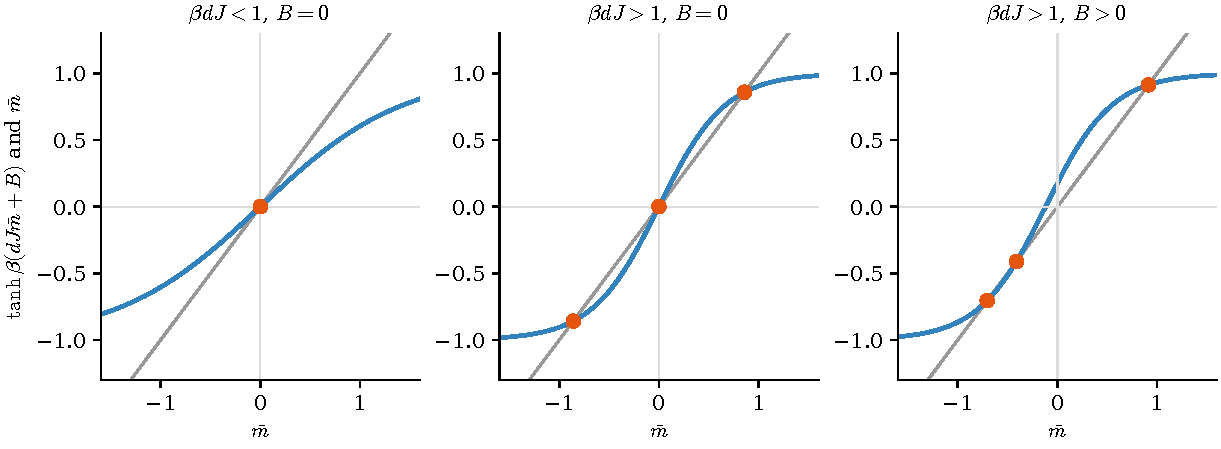
\includegraphics[width=0.98\linewidth]{fig/ising-tanh.pdf}
  \caption{Graphical solution of the mean-field equation \eqref{ising-sc}: intersections of $\tanh\beta(dJ\bar m+B)$ with the diagonal. Left: high temperature, one solution at $\bar m=0$. Middle: low temperature at $B=0$, three solutions, of which $\bar m=0$ is a maximum of $s$ and $\pm\bar m$ are degenerate minima. Right: low temperature with $B>0$, three solutions, with the positive one the global minimum.}
  \label{fig:ising-tanh}
\end{figure}

\emph{Self-consistency (an aside).} There is another route to \eqref{ising-sc}, which is the form in which mean-field theory usually appears and which we will use in Section \ref{sec:MFT}. Look at the effective field felt by a single spin $s_i$:
%
\begin{equation}
    B^{\rm eff}_i = -\frac{\pd E}{\pd s_i} = J\sum_{j\sim i}s_j + B \;\approx\; dJ\,m + B\,.
\end{equation}
%
A single spin in this field has partition function $Z_i = \sum_{s_i=\pm1}e^{\beta B^{\rm eff}s_i} = 2\cosh\beta(dJm+B)$ and mean $\E(s_i) = \beta^{-1}\pd_B\log Z_i = \tanh\beta(dJm+B)$. If the approximation is to be consistent, the average that comes out must equal the average we put in, $m = \E(s_i)$, and that is \eqref{ising-sc}. Solve the one-body problem in the average environment, then demand that the average be reproduced: this is the prototype of every mean-field theory.

\subsection{Phases and phase transitions}
\label{sec:phase-transitions}

Now we analyze the structure of the minima of $s(m)$, which control where the probability concentrates, as $\beta$, $J$, and $B$ are varied. Taylor-expanding the entropy, $h(m) = \log 2 - \frac{m^2}{2} - \frac{m^4}{12} - \ldots$, the action is
%
\begin{equation}
    s(m) \;\approx\; \text{const} - B\,m + \frac{1}{2}\big(\beta^{-1} - dJ\big)\,m^2 + \frac{\beta^{-1}}{12}\,m^4 + \ldots \label{landau}
\end{equation}
%
This expansion of a free energy in powers of an order parameter is called a \emph{Landau theory}, and the qualitative analysis below depends only on its form, not on the microscopic model behind it.

\emph{The ordered phase and a first-order transition.} Take $dJ > \beta^{-1}$: the coupling beats the temperature, the quadratic coefficient in \eqref{landau} is negative, and $s(m)$ is a double well (\cref{fig:ising-wells}). The system wants to be ordered, with neighboring spins aligned; but aligned which way? The field decides. For $B<0$ the global minimum is near $m=-1$, for $B>0$ near $m=+1$, and at $B=0$ the two minima are exactly degenerate. As $B$ is swept through $B_c = 0$, the magnetization the system displays jumps from $\bar m\approx -1$ to $\bar m\approx +1$. This is a \emph{first-order phase transition}.

\begin{figure}[ht]
  \centering
  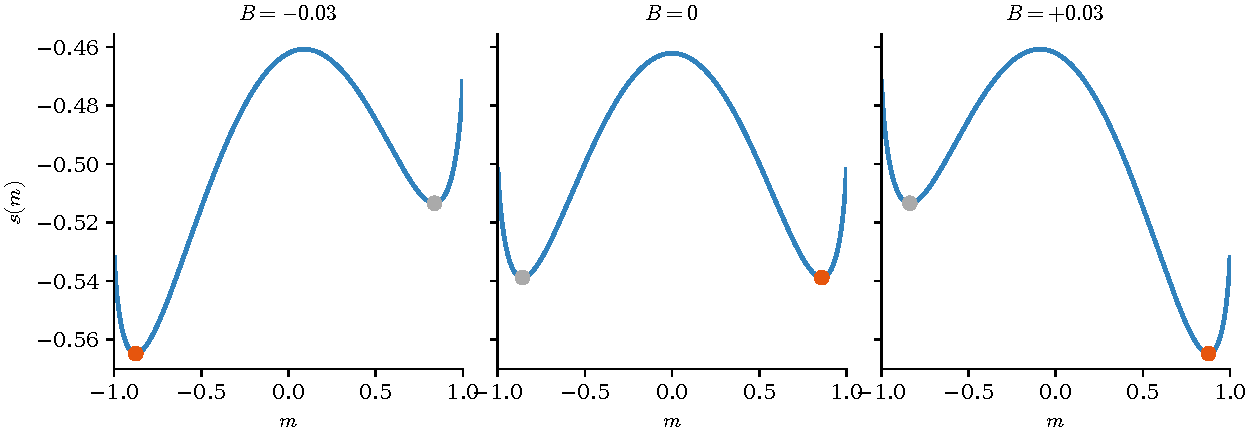
\includegraphics[width=0.98\linewidth]{fig/ising-wells.pdf}
  \caption{The action $s(m)$ of \eqref{ising-action} in the ordered phase ($\beta dJ = 1.5$), for a negative, zero, and positive external field. The two minima tilt with $B$; the global minimum (orange) switches sides at $B=0$. The suppressed minimum (grey) survives as a metastable state.}
  \label{fig:ising-wells}
\end{figure}

The structure of this transition is universal, in the sense that it follows from two isolated minima crossing and not from any detail of the model. Consider the expected magnetization, which by \eqref{R-cumulants} is a derivative of the free energy with respect to the field:
%
\begin{equation}
    \E(m) = \frac{1}{N}\sum_i\E(s_i) = -\frac{1}{\beta}\frac{\pd\varphi}{\pd B}\,.
\end{equation}
%
At finite $N$, the two minima of $s$ are two competing \emph{phases}, and $\E(m)$ is a probability-weighted average of their magnetizations. As $N\to\infty$ the saddle-point approximation puts all the weight on the lower minimum, so $\E(m)$ develops a discontinuity at $B_c$, and $\varphi$ itself develops a kink (\cref{fig:ising-firstorder}, left). \emph{A discontinuity in a first derivative of the free-energy density, in the thermodynamic limit, is the definition of a first-order transition.} Its second derivative, the \emph{susceptibility}
%
\begin{equation}
    \chi := \frac{\pd\,\E(m)}{\pd B} = -\frac{1}{\beta}\frac{\pd^2\varphi}{\pd B^2} = N\beta\,\mathrm{Var}(m)\,,
\end{equation}
%
is a peak whose height grows like $N$ and whose width shrinks like $1/N$: a nascent delta function (\cref{fig:ising-firstorder}, right). Genuine non-analyticity can occur only at $N=\infty$: at finite $N$ the partition function is a finite sum of analytic functions of $B$, so everything is smooth, and what one sees is a rapid \emph{crossover} that sharpens as $N$ grows. Watching the peak in $\chi$ grow with $N$, rather than saturate, is the standard numerical diagnostic that separates a true transition from a crossover. \Cref{ex:anatomy} works out the shapes of these curves for a general first-order transition; they are worth remembering whenever ``emergent capabilities'' in models of growing size are under discussion (Section \ref{sec:emergence}).

\begin{figure}[ht]
  \centering
  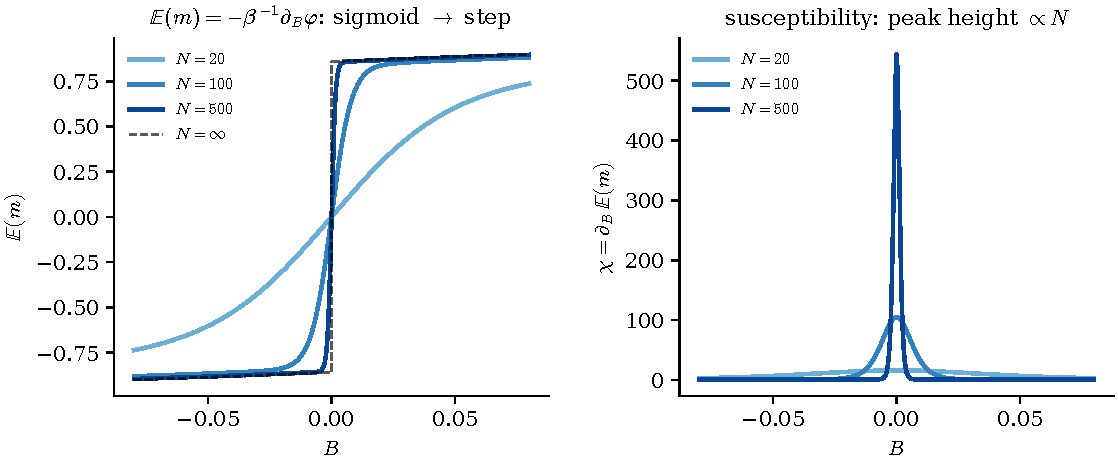
\includegraphics[width=0.98\linewidth]{fig/ising-firstorder.pdf}
  \caption{Fingerprints of a first-order transition, in the mean-field Ising model at $\beta dJ = 1.5$, computed from the one-dimensional integral \eqref{ising-action} at finite $N$. Left: the expected magnetization as a function of the field is a sigmoid of width $\propto 1/N$, sharpening into a step. Right: the susceptibility $\chi = \pd_B\E(m)$ is a peak of height $\propto N$ and width $\propto 1/N$.}
  \label{fig:ising-firstorder}
\end{figure}

\emph{Metastability and hysteresis.} The suppressed minimum in \cref{fig:ising-wells} does not disappear when it stops being the global one. A system that starts there and evolves by local dynamics (flipping one spin at a time) must climb over the barrier to reach the true minimum, which takes a time exponential in $N$. In practice the system stays in the \emph{metastable} phase until the field is pushed well past $B_c$, and the transition observed dynamically \emph{lags} the thermodynamic one. This is \emph{hysteresis}, familiar from real magnets. It is the reason the ``$\beta\leftrightarrow$ training time'' analogy of Section \ref{sec:Bayes} must be handled with care at first-order transitions, and we will meet it again in the guise of delayed generalization (grokking) in Section \ref{sec:grok}.

\emph{A second-order transition.} An \emph{$n$-th order} phase transition is a discontinuity in the $n$-th derivative of the free-energy density as $N\to\infty$. The Ising model has a second-order transition too, at fixed $B=0$, as the temperature $T=\beta^{-1}$ crosses $T_c = dJ$ (\cref{fig:ising-secondorder}). Here nothing crosses anything: the single basin at $m=0$ flattens and splits into two symmetric ones. The quadratic coefficient in \eqref{landau} changes sign at $T_c$, and the minima sit at
%
\begin{equation}
    \bar m^2 = 3\,(\beta dJ - 1) \;\approx\; 3\,\Big(1-\frac{T}{T_c}\Big)\qquad (T\lesssim T_c)\,, \label{ising-exponent}
\end{equation}
%
so the order parameter $\bar m \propto (T_c - T)^{1/2}$ moves \emph{continuously} but not smoothly; $\varphi$ and $\pd_T\varphi$ are continuous, and the discontinuity sits in $\pd_T^2\varphi$ (the heat capacity). The point $(T,B) = (T_c,0)$ is a \emph{critical point}. Below it the two ordered states $\pm\bar m$ are exact mirror images, and the system must pick one: this is \emph{spontaneous symmetry breaking}, the $\mathbb Z_2$ symmetry $s\to -s$ of the energy at $B=0$ being broken by the state. The exponent $\frac{1}{2}$ in \eqref{ising-exponent} is an example of a \emph{critical exponent}. Mean-field theory predicts it in every dimension, and it is wrong in low dimension: the exact value is $\frac{1}{8}$ in $D=2$ (Onsager), and there is no transition at all in $D=1$. Mean-field exponents become exact for $D\geq 4$. Understanding why is the subject of the renormalization group, for which see \cite{TongSFT}.

\begin{figure}[ht]
  \centering
  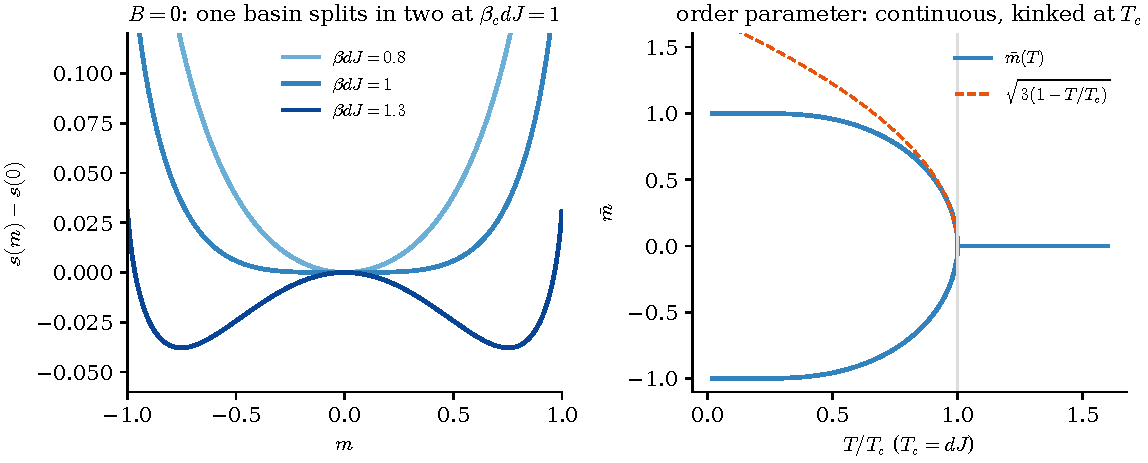
\includegraphics[width=0.98\linewidth]{fig/ising-secondorder.pdf}
  \caption{The second-order transition of the mean-field Ising model at $B=0$. Left: the action $s(m)$ for temperatures above, at, and below $T_c = dJ$; a single basin flattens and splits into two symmetric ones. Right: the resulting magnetization $\bar m(T)$, continuous at $T_c$ but with the square-root singularity \eqref{ising-exponent} (dashed).}
  \label{fig:ising-secondorder}
\end{figure}

\emph{Back to learning.} In the Bayesian model of Section \ref{sec:Bayes}, the natural control parameter is $n\beta$, the amount of data or training. The Ising analogue is sweeping $\beta$ at fixed $B=0$, which sees the second-order transition. First-order transitions in learning arise when two qualitatively different families of solutions compete, one entropically favored and one favored by the data; the Ising perceptron of Section \ref{sec:ising} is the cleanest example. Before turning to it, the following exercise establishes what \emph{every} first-order transition looks like at finite $N$.

\begin{exercise}[Anatomy of a first-order transition]
\label{ex:anatomy}
\important
Consider any system whose partition function has the form $Z(B) = \int d\theta\, e^{-N E(\theta,B)}$, depending on \emph{some} hyperparameter $B$. Here $B$ could be the inverse temperature, an external field, or the load $\alpha$ of Section \ref{sec:ising}; we have absorbed $\beta$ into $E$ to keep the setup general. Suppose that $E(\theta,B)$ has exactly two isolated minima, at $\theta_1$ and $\theta_2$. Then at large $N$ the integral is dominated by two competing phases. Letting $U_1,U_2$ be small neighborhoods of $\theta_1,\theta_2$,
%
\begin{equation}
    Z(B) \;\approx\; \int_{U_1} d\theta\,e^{-N E(\theta,B)} + \int_{U_2} d\theta\,e^{-N E(\theta,B)} \;=\; e^{-N\varphi_1(B)} + e^{-N\varphi_2(B)}\,, \label{two-branch-Z}
\end{equation}
%
with $\varphi_i(B) = -\frac{1}{N}\log\int_{U_i}d\theta\,e^{-NE(\theta,B)} = E(\theta_i,B) + o(1)$ the free-energy densities of the two basins. Suppose further that as $B$ crosses a critical value $B_c$ the two minimum values cross: $\varphi_1(B_c) = \varphi_2(B_c)$ with $\varphi_1'(B_c)\neq\varphi_2'(B_c)$, where a prime denotes $\pd_B$.
\begin{enumerate}
    \item \emph{Occupation.} Show that the probability of finding the system in basin $i$ is
    %
    \begin{equation}
        p_i(B) = \frac{e^{-N\varphi_i(B)}}{e^{-N\varphi_1(B)}+e^{-N\varphi_2(B)}}\,, \label{p-weights}
    \end{equation}
    %
    and that, expanding to first order in $\Delta B := B - B_c$,
    %
    \begin{equation}
        p_2(B) \approx \frac{1}{1+e^{-N\,\Delta\varphi'\,\Delta B}}\,,\qquad \Delta\varphi' := \varphi_1'(B_c) - \varphi_2'(B_c)\,, \label{p-logistic}
    \end{equation}
    %
    a logistic function of $N\,\Delta\varphi'\,\Delta B$. Over what window of $B$ does the system switch allegiance?
    \item \emph{First derivative.} Show from \eqref{two-branch-Z} that
    %
    \begin{equation} \label{dF-sigmoid}
        \frac{\pd\varphi}{\pd B} \;\approx\; p_1(B)\,\varphi_1'(B_c) + p_2(B)\,\varphi_2'(B_c)\,,
    \end{equation}
    %
    the probability-weighted average of the branch slopes. Sketch it at finite $N$ and at $N=\infty$: a sigmoid of height $\Delta\varphi'$ sharpening into a jump. The kink in $\varphi$ itself is the defining discontinuity of a first-order transition. Show also, directly from the integral, that $\pd_B\varphi = \E\big[\pd_B E(\theta,B)\big]$: the observable that jumps is the one conjugate to the control parameter. When $B=\beta$ it is the energy, and the jump is the \emph{latent heat}; for the Ising model with $B$ the field, it is the magnetization.
    \item \emph{Second derivative.} Using $\pd_B p_1 = -\pd_B p_2 = -N p_1p_2\,\Delta\varphi'$ (verify this), show that
    %
    \begin{equation} \label{chi-peak}
        -\frac{\pd^2\varphi}{\pd B^2} \;=\; N\,p_1p_2\,(\Delta\varphi')^2 \;-\; p_1\varphi_1'' - p_2\varphi_2''\,.
    \end{equation}
    %
    Sketch this curve. Near $B_c$, where $p_1p_2\approx\frac{1}{4}$, the first term is a peak of height $\sim N(\Delta\varphi')^2/4$ and width $\sim 1/(N\Delta\varphi')$, which converges to a delta function as $N\to\infty$. Show also that when $\CO(\theta) = \pd_BE(\theta,B)$ does not depend on $B$, $-\pd_B^2\varphi = N\,\mathrm{Var}(\CO)\geq 0$. (For $B=\beta$ this is the heat capacity; for the Ising field it is the susceptibility.)
    \item \emph{Plot it.} Take the minimal model $\varphi_1(B) = a\,(B-B_c)$, $\varphi_2 = 0$ and plot $\varphi$, $\pd_B\varphi$, and $-\pd_B^2\varphi$ for a few values of $N$. (Use a numerically stable $\log(e^x+e^y)$.) Watching the peak grow with $N$ rather than saturate is the standard diagnostic separating a true transition from a smooth crossover.
\end{enumerate}
\end{exercise}

\subsection{The Ising perceptron: a first-order transition in learning}
\label{sec:ising}

We close the physics part of this section with a complete statistical-mechanics analysis of a learning problem, built to run in parallel with the Ising magnet. It is the simplest model we know in which \emph{more data} produces a genuine phase transition to \emph{perfect generalization}, and it goes back to Gy\"orgyi \cite{gyorgyi1990first}; see \cite[Chapter 7]{engel2001statistical}. It is presented as a walk-through exercise; solutions are in Appendix \ref{app:solutions}, but try each part before reading them.

\emph{Setup.} A \emph{teacher} is a fixed vector of binary weights $\theta^*\in\{\pm1\}^N$. Inputs are Gaussian, $x\sim\CN(0,I_N)$, and the teacher labels them by
%
\begin{equation}
    y(x) = \mathrm{sign}(\theta^*\cdot x)\,. \label{perc-teacher}
\end{equation}
%
A \emph{student} is another binary vector $\theta\in\{\pm1\}^N$, guessing labels the same way, $f_\theta(x) = \mathrm{sign}(\theta\cdot x)$. This model is called the \emph{Ising perceptron}, because its weights take the values of Ising spins. We observe $n$ examples $(x^\mu,y^\mu)$ with $y^\mu = y(x^\mu)$, and do Bayesian learning at zero temperature with a uniform prior, in the sense of Section \ref{sec:loss-likelihood}: the per-sample loss is $0$ if the student classifies the example correctly and $\infty$ otherwise, so the posterior is uniform on the students that classify \emph{every} example correctly. Since teacher and student agree on $x$ exactly when $y(x)\,(\theta\cdot x)>0$,
%
\begin{equation}
    p(\theta) \;\propto\; \prod_{\mu=1}^n\Theta\big(y^\mu\,(\theta\cdot x^\mu)\big)\,,\qquad
    Z = \frac{1}{2^N}\sum_{\theta\in\{\pm1\}^N}\;\prod_{\mu=1}^n\Theta\big(y^\mu\,(\theta\cdot x^\mu)\big)\,, \label{perc-Z}
\end{equation}
%
with $\Theta(u) = 1$ for $u>0$ and $0$ otherwise. With the factor $1/2^N$, $Z$ is the fraction of all students consistent with the data. Both $N$ and $n$ will be taken large, at fixed ratio: the \emph{load}
%
\begin{equation}
    \alpha := \frac{n}{N}\,, \label{load}
\end{equation}
%
the number of examples per parameter, is the control parameter of the problem.

\begin{exercise}[The Ising perceptron]
\label{ex:ising}
\important
\begin{enumerate}
    \item \emph{The order parameter is a magnetization.} Define the \emph{overlap} $R(\theta) = \frac{1}{N}\theta\cdot\theta^*\in[-1,1]$ and the alignment variables $s_i := \theta_i\theta_i^*\in\{\pm1\}$. Show that $R = \frac{1}{N}\sum_i s_i$: the overlap \emph{is} the magnetization of the spins $s_i$. Learning the teacher means magnetizing them to $R=1$.
    \item \emph{Generalization error.} Show that a student at overlap $R$ misclassifies a fresh Gaussian input with probability
    %
    \begin{equation}
        \varepsilon(R) = \frac{\arccos R}{\pi}\,. \label{eps-of-R}
    \end{equation}
    %
    \hint{project $x$ onto the plane spanned by $\theta$ and $\theta^*$; the projection is an isotropic two-dimensional Gaussian, and the two decision boundaries are diameters meeting at angle $\arccos R$. When do the signs disagree?}
    \item \emph{Entropy: the same $h$ as the magnet.} Show that the number of students at overlap $R$ is $\binom{N}{\frac{1+R}{2}N}$, so that by Stirling's formula
    %
    \begin{equation}
        \begin{aligned}
        \frac{1}{N}\log\#\{\theta : R(\theta) = R\} \;\to\; h(R) &= \log 2 - \frac{1-R}{2}\log(1-R) \\ &\quad - \frac{1+R}{2}\log(1+R)\,,
        \end{aligned}
    \end{equation}
    %
    \emph{identical} to the magnet's entropy \eqref{ising-entropy} with $m\to R$.
    \item \emph{Push forward to one variable.} Average $Z$ over datasets. The examples are independent, and each is classified correctly by a student at overlap $R$ with probability $1-\varepsilon(R)$, so
    %
    \begin{equation}
        \E_x Z = \frac{1}{2^N}\sum_\theta\big(1-\varepsilon(R(\theta))\big)^n\,.
    \end{equation}
    %
    Trade the sum over $\theta$ for an integral over $R$ using (c), and show that at fixed load $\alpha$ and large $N$,
    %
    \begin{equation}
        \E_x Z \;\approx\; \int_{-1}^{1}dR\; e^{-N\,s(R)}\,,\qquad s(R) = \log 2 - h(R) - \alpha\log\big(1-\varepsilon(R)\big)\,. \label{perc-action}
    \end{equation}
    %
    This is the exact analogue of the magnet's \eqref{ising-action}: an entropy term counting states, and a ``field'' term rewarding alignment. The aligning field is now the \emph{data}, and its strength is the load $\alpha$. (Averaging $Z$ rather than $\log Z$ is the annealed approximation \eqref{annealed-swap}. It preserves all the qualitative structure here and shifts the numbers only slightly; \cref{app:replica} explains how to do the exact calculation.)
    \item Plot $s(R)$ for several values of $\alpha$ and locate its critical points. Do you expect a phase transition? At which $\alpha$?
    \item \emph{The teacher basin.} $R=1$ is the perfectly aligned state, where the student is the teacher. Show that $s(1) = \log 2$ for \emph{every} $\alpha$ (zero entropy, but zero data cost), and that $R=1$ is always a local minimum: writing $\delta = 1-R$, deviating from the teacher gains entropy $\sim\frac{\delta}{2}\log(1/\delta)$ but costs data-fit $\alpha\varepsilon\sim\alpha\sqrt{2\delta}/\pi$ (expand $\arccos$), and $\sqrt\delta\gg\delta\log(1/\delta)$. This differs from the magnet, where the aligned state sat at the bottom of a smooth well and was not always a minimum.
    \item \emph{The interior basin, the crossing, and the transition.} At $\alpha=0$, $s$ is minimized at $R=0$ with $s(0) = 0 < s(1)$: the disordered cloud of typical students dominates. As $\alpha$ grows, this interior minimum $R^*(\alpha)$ drifts toward $1$ and its value rises. Numerically, find the load $\alpha_c$ at which the two basins exchange dominance, $s(R^*(\alpha_c)) = s(1)$. You should find $\alpha_c\approx 1.45$, with the interior minimum still at $R^*\approx 0.70$, that is, generalization error $\varepsilon^*\approx 0.25$. Conclude that at $\alpha_c$ the typical student jumps from $25\%$ error to \emph{zero} error: a first-order transition to perfect generalization. Then connect to \cref{ex:anatomy} with $\alpha$ as the control parameter: what do $\pd_\alpha\varphi$ and $-\pd_\alpha^2\varphi$ look like at finite $N$, and what plays the role of the latent heat? Finally, find the load at which the interior minimum disappears altogether, and explain what happens in between in the light of the metastability discussion of Section \ref{sec:phase-transitions}.
    \item \emph{The dictionary.} Complete the table:
    \begin{center}
    \small
    \renewcommand{\arraystretch}{1.3}
    \begin{tabular}{l|l}
        \textbf{Ising magnet} & \textbf{Ising perceptron} \\\hline
        spins $s_i\in\{\pm1\}$ & alignments $s_i = \theta_i\theta_i^*\in\{\pm1\}$ \\
        magnetization $m$ & overlap $R$ \\
        entropy $h(m)$ & entropy $h(R)$ \emph{(the same function)} \\
        aligning field $B$ & ? \\
        knob swept across the transition & ? \\
        ordered phase $\E(m)\approx\pm1$ & ? \\
        jump in $\E(m)$ as a function of $B$ & ? \\
    \end{tabular}
    \end{center}
    Also articulate one structural \emph{difference}: in the magnet the two competing minima are symmetry partners; what are they here, and which ingredient of (c) made a sharp transition possible at all? (What would change for spherical weights $\theta\in\R^N$, $|\theta|^2 = N$, where the slice at overlap $R$ has volume $\propto(1-R^2)^{N/2}$? \Cref{app:sph-perceptron} works this case out.)
\end{enumerate}
\end{exercise}

\subsection{Comparison with QFT}
\label{sec:QFT-comparison}

This short subsection is a translation guide, aimed mainly at readers arriving from high-energy or condensed-matter physics --- if the words ``action'' and ``path integral'' mean more to you than ``posterior'' and ``marginal likelihood,'' read on; everyone else may safely skip ahead.

Nearly everything in these notes lives, in the first instance, in \emph{Euclidean equilibrium statistical mechanics}: probability distributions of Boltzmann--Gibbs form $P \propto e^{-\beta E}$, partition functions, free energies. For a field theorist, a partition function with sources,
%
\begin{equation}
    Z[J] = \int \mathcal{D}\phi\; e^{-S[\phi] \,+ \int J\,\phi}\,,
\end{equation}
%
is a moment generating functional; its logarithm generates connected correlation functions (cumulants); the action $S$ encodes the microscopic rules of the system, and a quadratic action means a free (Gaussian) theory, with everything else treated by perturbing around it. In these notes the role of the field $\phi$ is played variously by the weights $\theta$ of a network, by an order parameter such as the magnetization $m$ or the overlap $R$ of Sections \ref{sec:ising-model} and \ref{sec:ising}, or --- most usefully --- by the network function $f(x)$ itself, with the input $x$ playing the role of the spacetime coordinate. Functional integrals over the network function are developed carefully in Sections \ref{sec:GP} and \ref{sec:NNGP-int}, and the reader coming from QFT will find many familiar ingredients there dressed up as learning theory: Wick's theorem, sources, cumulants, effective actions.

If your instincts were trained on Lorentzian signature, picture everything here as already Wick-rotated. There is no $i/\hbar$: the weights $e^{-S}$ are real and positive, as after the standard continuation
%
\begin{equation}
    Z_{\rm QFT} =  \int \mathcal{D} \phi\; e^{\frac{i}{\hbar} S[\phi]} \;\;\xrightarrow{\;\tau\,=\,it\;}\;\; Z_{\rm E} = \int \mathcal{D} \phi\; e^{- S_E [\phi]/\hbar}\,.
\end{equation}
%
The role of $\hbar$ --- the parameter controlling the size of fluctuations around saddle points --- is played here by temperature, or by $1/N$ at large width, or by $1/n$ at large sample size.

When we eventually study the \emph{dynamics} of training as a field theory in Section \ref{sec:DMFT}, a genuinely real-time formalism does appear --- a path integral over trajectories with a causal structure and a response field. That's the closest object in these notes to a Lorentzian field theory, and is precisely the Martin--Siggia--Rose construction of non-equilibrium statistical mechanics.

For readers who would like physics references alongside the learning-theory ones: David Tong's lecture notes \cite{TongStatPhysics,TongSFT,TongKineticTheory,TongQFT} are a friendly introduction to statistical physics, statistical field theory, kinetic theory, and QFT respectively; Lancaster and Blundell \cite{lancaster2014quantumGifted} is a gentle conceptual route into QFT; Altland and Simons \cite{altlandCondensedMatterField2010} bridges toward condensed-matter field theory (and contains the Langevin/MSRJD material used in Section \ref{sec:DMFT}); Pathria \cite{pathriaStatisticalMechanics2011} is a standard graduate statistical mechanics text; Goldenfeld \cite{goldenfeldLecturesPhaseTransitions2018a} is the classic on phase transitions and the renormalization group; and Zinn-Justin \cite{zinn2002quantum} is the encyclopedic reference for the functional formalism.





\section{Large width at initialization: the Gaussian process limit}
\label{sec:init}

The next few sections are all about different limits in neural networks, in which some parameter(s) become large. Such limits are where physical/statistical analyses really shine. Studying them teaches some basic lessons about how we should (and should not) initialize networks, and how to choose other hyperparameters. It also leads to analytically solvable models that display many properties we see in practice: lazy vs. rich learning, double descent, phase transitions, scaling laws for optimal learning. For further pedagogical references on much of this material, we recommend \cite{roberts2022principles,spiliopoulos2025foundations,ringel2025applications} and the online lectures \cite{hanin2026mdl}.

We'll begin in this section with a classic result \cite{neal1996bayesian, lee2018deep, yang2019tensorprograms1, hanin2023random} about increasing the width of a network at fixed depth and training-sample size.

\smallskip
Modern neural networks are more sophisticated than the simple MLP's discussed here, but they share many of the same features. Layer norms solve the problem of trainability at large depth, but the analysis of rich/lazy regimes, feature learning, and hyperparameter scaling is still relevant. See \emph{e.g.} the discussion of $\mu P$ in Section \ref{sec:MFT-practice}.




\subsection{Notation}
\label{sec:setup}

We'll use the following notation for neural networks and training data.

\begin{itemize}
    \item $\theta\in \R^P$ trainable network parameters (weights, biases)
    \item $(x^\mu,y^\mu)_{\mu=1}^n$ training data samples, with $x^\mu\in \R^d$ and $y^\mu\in \R$ (unless otherwise stated)
    \item $f_\theta:\R^d\to \R$ network function
\end{itemize}

\noindent For MLP's in particular (also called FCN's = fully connected networks)
\begin{itemize}
    \item $\{z_i^{(\ell)}\}_{i=1}^{N_\ell}$ pre-activations in layer $\ell\in \{0,...,L+1\}$
    \item $L=$ number of hidden layers (depth); $N_\ell = $ width of $\ell$'th layer; $N_0=d$ and $N_{L+1}=1$. We will often take constant hidden depth, $N_1=...=N_L=N$.
    \item $\phi:\R\to \R$ activation function (assumed the same in all layers except the first) 
    \item network recursion $z_i^{(\ell)} = \begin{cases} \frac{1}{\sqrt{N_{\ell-1}}}\sum_{j=1}^{N_{\ell-1}}w^{(\ell)}_{ij}\,\phi(z^{(\ell-1)}_j)+ b^{(\ell)}_i & \ell\geq 2 \\[.2cm]  \frac{1}{\sqrt d}\sum_{j=1}^{d}w^{(1)}_{ij}\,x_j+ b^{(1)}_i & \ell = 1 \end{cases}$ \\
    with $z^{(0)} = x$ and $z^{(L+1)} = f$; parameters are $\theta = \{w^{(\ell)},b^{(\ell)}\}_{\ell=1}^{L+1}$\,. The explicit factors of $1/\sqrt{N_{\ell-1}}$ are a normalization convention, explained in Section \ref{sec:basicscaling}: with them in place, all weights and biases can be taken of order one.
\end{itemize}


\subsection{Normalizing the network}
\label{sec:basicscaling}

Consider a fully connected network of depth $L$ with layer widths $N_\ell$ as in Section \ref{sec:setup}. Suppose we keep $L$ fixed but make the $N_\ell$ very large. Suppose also that the network is initialized randomly, with all weights and biases drawn independently from normal distributions of \emph{order-one} variance,
%
\begin{equation} \label{init-O1}
    w_{ij}^{(\ell)} \sim \CN(0,\sigma_w)\,,\qquad b_i^{(\ell)}\sim \CN(0,\sigma_b)\,,
\end{equation}
%
with $\sigma_w,\sigma_b$ fixed as the widths grow. (Here and throughout, $\CN(0,\sigma)$ denotes a Gaussian of \emph{variance} $\sigma$. Letting the variances depend on the layer changes nothing below.) The question is how to normalize the sums in the network recursion so that preactivations stay of order one from layer to layer. From
%
\begin{equation}
   z_i^{(\ell)} = \frac{1}{\sqrt{N_{\ell-1}}}\, w_i^{(\ell)} \cdot \phi(z^{(\ell-1)}) + b_i^{(\ell)}
\end{equation}
%
(where we've written $w_i=(w_{i,1},...,w_{i,N_{\ell-1}})$ and $z^{(\ell-1)} = (z^{(\ell-1)}_1,...,z^{(\ell-1)}_{N_{\ell-1}})$ as vectors) we get
%
\begin{align}
    \text{Var}(z_i^{(\ell)}) &= \frac{1}{N_{\ell-1}}\sum_{j=1}^{N_{\ell-1}} \text{Var}\big(w_{ij}^{(\ell)}\big)\, \E\Big[\phi\big(z_j^{(\ell-1)}\big)^2\Big] \;+\; \text{Var}\big(b_i^{(\ell)}\big) \notag \\
    &= \sigma_w \cdot \frac{1}{N_{\ell-1}}\sum_{j=1}^{N_{\ell-1}}\Big( \text{Var}\big(\phi(z_j^{(\ell-1)})\big)+\E\big[\phi(z_j^{(\ell-1)})\big]^2\Big) +\sigma_b\,.
\end{align}
%
Here we've conditioned on the previous layer, and used that for independent mean-zero $X$ and arbitrary $Y$, $\text{Var}(XY) = \text{Var}(X)\,\E[Y^2]$, along with additivity of variance for independent summands. The average in the second line involves only the activation function and the order-one preactivations of the previous layer, so it stays of order one as $N_{\ell-1}\to\infty$. (We'll sharpen this estimate in Section \ref{sec:chaos}.) Thus
%
\begin{equation} \label{fanin}
    \text{Var}(z_i^{(\ell)}) \approx \sigma_w\cdot O(1) + \sigma_b = O(1)\,.
\end{equation}
%
The prefactor $1/\sqrt{N_{\ell-1}}$, the square root of the number of inputs (the ``fan-in'') feeding each neuron, is exactly what keeps the preactivations of order one at large width. We call this the \emph{fan-in normalization}; it goes back to LeCun and collaborators in the 90's \cite{lecun1998efficient}. In Section \ref{sec:train} it will also be called the \emph{NTK normalization}, and in Section \ref{sec:MFT} we will meet the alternative \emph{mean-field normalization}, in which the output layer carries $1/N$ instead of $1/\sqrt N$.

\smallskip
\noindent\textbf{Remark (other conventions).} Common practice, and the convention of much of the literature, is to put no explicit prefactors in the network and instead to initialize with width-dependent variances,
%
\begin{equation} \label{init-fanin-var}
    \tilde w^{(\ell)}_{ij} := \frac{w^{(\ell)}_{ij}}{\sqrt{N_{\ell-1}}} \;\sim\; \CN\Big(0,\frac{\sigma_w}{N_{\ell-1}}\Big)\,.
\end{equation}
%
At initialization the two conventions describe \emph{exactly} the same distribution of network functions: \eqref{init-fanin-var} is a change of variables on parameter space, and the network function is the same function of $x$. Everything in this section, which concerns initialization only, is insensitive to the choice. During training, however, the two conventions are \emph{not} equivalent: gradient descent is not invariant under rescaling coordinates on parameter space, as we will explain in Section \ref{sec:NTK-const}. Keeping every parameter of order one, with the factors of $N$ displayed explicitly in the network function, makes the comparison between different scaling limits transparent, and it is the convention we use throughout these notes. When reading the literature, expect the factors of $N$ to sit in the variances instead, and translate with \eqref{init-fanin-var}.

\subsection{Gaussian processes}
\label{sec:GP}


A \emph{Gaussian process} $f:\R^m\to \R$ with mean function $\mu$ and covariance kernel $K$ is a random function such that on any $p$ inputs $(x^1,...,x^p)\in (\R^m)^p$ the vector of function values is Gaussian
%
\begin{equation} \begin{pmatrix} f(x^1) \\ \vdots \\ f(x^p) \end{pmatrix} \sim \CN \left( \begin{pmatrix} \mu(x^1) \\ \vdots \\ \mu(x^p) \end{pmatrix}, \begin{pmatrix} K(x^1,x^1) & \cdots & K(x^1,x^p) \\ \vdots & \ddots & \vdots \\ K(x^p,x^1) & \cdots & K(x^p,x^p) \end{pmatrix} \right)\,.  \end{equation}
%
Here $\mu:\R^m\to \R$ and $K:\R^m\times \R^m\to \R$ are fixed, deterministic functions that control the mean and covariance of any tuple of values of $f$. The function $K$, often called the kernel of the process, is symmetric: $K(x,x')=K(x',x)$.

Let `$dx$' denote a measure on $\R^m$ (it need not be the usual Lebesgue measure). If $K$, as integral kernel, has an inverse $K^{-1}$ satisfying
%
\begin{equation} \int dx' K^{-1}(x,x') K(x',x'') = \delta(x-x'') \end{equation}
%
then there's also a ``physics definition'' of a Gaussian process. It's not entirely rigorous, as it invokes multi-dimensional functional integrals. Mathematically, it's best thought of as a heuristic tool, which comes with a package of axiomatic manipulations whose actual results can (and should) all be fully justified by other means. The manipulations are all quite intuitive, though, and familiar to quantum field theorists, so we mention this formalism here. The idea is that, just like a single Gaussian variable `$z$' has a probability measure
%
\begin{equation} P(z) = \frac{1}{Z}e^{-\frac{1}{2}K^{-1}(z-\mu)^2}\,,\qquad Z = \int dz\,e^{-\frac{1}{2}K^{-1}(z-\mu)^2} = \sqrt{2\pi K}\,, \end{equation}
%
a Gaussian process $f$ has a (non-rigorous) measure
%
\begin{align} P[f] &= \frac{1}{Z}e^{\textstyle-\frac{1}{2} \int dx\,dx'\, (f(x)-\mu(x)) K^{-1}(x,x')(f(x')-\mu(x'))}\,, \notag \\ 
Z &\; \text{`='} \int Df\, e^{\textstyle-\frac{1}{2} \int dx\,dx'\, (f(x)-\mu(x)) K^{-1}(x,x')(f(x')-\mu(x'))}\,. \end{align}
%
If the kernel and the measure theory on the input space $\R^m$ are nice enough to allow $K$ to be diagonalized, with a discrete basis of orthonormal eigenfunctions $\{\phi_k(x)\}_{k=1}^\infty$ and eigenvalues $\lambda_1\geq \lambda_2\geq\ldots > 0$ (so that $K^{-1}$ has eigenvalues $1/\lambda_k$), then $P[f]$ can be understood as an infinite-dimensional Gaussian. Writing $f(x)-\mu(x) = \sum_{k=1}^\infty a_k \phi_k(x)$,
%
\begin{equation} P[f] = \frac{1}{Z} e^{\textstyle -\frac{1}{2}\sum_{k=1}^\infty a_k^2/\lambda_k}\,,\qquad Z = \prod_{k=1}^\infty (2\pi \lambda_k)^{1/2}\,.\end{equation}

One virtue of the physics formalism is that it organizes expectation values of products of $f(x)$'s. Let $\mu=0$ for simplicity (to generalize to any $\mu$, just shift $f\mapsto f-\mu$ below). Let $J:\R^m\to \R$ be an arbitrary (nice...) function and define
%
\begin{equation} Z[J] = \int Df\, e^{\textstyle -\frac{1}{2}\int dx\,dx'\, f(x)K^{-1}(x,x')f(x') + \int dx\, J(x)f(x)}\,. \label{ZJ}\end{equation}
%
The integral evaluates formally to
%
\begin{equation} Z[J] = Z[0] \cdot e^{\textstyle \frac{1}{2} \int dx\,dx'\, J(x) K(x,x') J(x')}\,. \label{ZJ-eval} \end{equation}
%
Then expectation values can be expressed via derivatives, which by \eqref{ZJ-eval} become
%
\begin{align} \E\big[ f(x^1)...f(x^p)\big] &= \frac{1}{Z[0]} \frac{\delta}{\delta J(x^1)}...\frac{\delta}{\delta J(x^p)} Z[J]\bigg|_{J=0} \\ &= \sum_{\text{pairs}\,\{i_1,i_2\}\cup...\cup\{i_{p-1},i_p\}=\{1,2,...,p\}}  \prod_{j=1}^{p/2} K(x^{i_{2j-1}},x^{i_{2j}})\,. \label{GP-prods}
\end{align}
%
The sum is over partitions of $\{1,...,p\}$ into pairs, and vanishes if $p$ is odd. Eqn. \eqref{GP-prods} is called Wick's Theorem in QFT, Isserlis's Theorem in probability (and it's correct, despite the non-rigorous derivation here).

\begin{exercise}[Wick's theorem]
\label{ex:wick}
If you haven't seen this before, derive \eqref{ZJ-eval} by completing the square in \eqref{ZJ}, and then derive \eqref{GP-prods} by differentiating. Check the first two cases explicitly: $\E[f(x^1)f(x^2)] = K(x^1,x^2)$, and $\E[f(x^1)f(x^2)f(x^3)f(x^4)] = K^{12}K^{34}+K^{13}K^{24}+K^{14}K^{23}$ (with $K^{ij}=K(x^i,x^j)$). How many terms appear at $p=6$?
\end{exercise}

Another virtue of the physics formalism is that it neatly connects \emph{higher cumulants} to \emph{deviations from Gaussianity}. In general, the $p$-th cumulant $\kappa_p(X_1,...,X_p)$ of random variables $X_1,...,X_p$ is defined recursively via
%
\begin{equation} \E(X_1\cdots X_p) = \sum_{\text{partition $\Pi$ of $\{1,...,p\}$}} \;\prod_{\text{blocks $\{i_1,...,i_k\}\subset \Pi$}} \kappa_k(X_{i_1},...,X_{i_k})   \end{equation}
%
For example, $\kappa_1(X)=\E(X)$, $\kappa_2(X_1,X_2)=\text{Cov}(X_1,X_2) = \E(X_1X_2)-\E(X_1)E(X_2)$. In physics, the $\kappa_p$'s are called connected correlation functions; they measure the part of a joint expectation that's not captured by expectations of subsets of the variables involved. For a Gaussian process,
%
\begin{equation} \kappa_2(f(x^1),f(x^2))=K(x^1,x^2)\,;\qquad \kappa_p(f(x^1),...,f(x^p)) = 0\quad\text{for all $p>2$}\,, \end{equation}
%
as can easily be seen directly from \eqref{GP-prods}, where joint expectations for $p>2$ all factor into products of pairs. Thus, nonvanishing higher $\kappa_p$'s are a measure of non-Gaussianity.

This appears in the functional-integral formalism as follows. Suppose that $f:\R^m\to \R$ is a random function that's governed by a functional probability distribution
%
\begin{equation} P[f] = \frac{1}{Z}\,e^{\textstyle-S[f]}\,, \end{equation}
%
for some functional $S:\{\text{functions } f\}\to \R$. (In physics $S$ is called the action.) Then just as in \eqref{ZJ}, we can introduce the generating function
%
\begin{align} Z[J] &:= \int Df\, e^{\textstyle-S[f]+\int dx\, J(x)f(x)} \notag \\ \Rightarrow\quad \E\big[f(x^1)...f(x^p)\big] &= \frac{1}{Z[0]}\frac{\delta}{\delta J(x^1)}...\frac{\delta}{\delta J(x^p)} Z[J]\bigg|_{J=0} \end{align}
%
The cumulants appear naturally as derivatives of $\log Z[J]$, otherwise known as the (sourced) free energy:
%
\begin{equation} \kappa_p(f(x^1),...,f(x^p)) = \frac{\delta}{\delta J(x^1)}...\frac{\delta}{\delta J(x^p)} \log Z[J] \bigg|_{J=0}\,, \end{equation}
%
which in turn means (formally) that
%
\begin{equation} Z[J] = \exp\sum_{p=1}^\infty \frac{1}{p!}\int dx^1...dx^p\, \kappa_p(f(x^1),...,f(x^p))\,J(x^1)...J(x^p)\,, \end{equation}
%
a generating function of cumulants. The original $S[f]$ is the inverse Legendre transform of $\log Z[J]$ (by definition of $Z[J]$). Expanded as a formal series in the cumulants (assuming they are small), and assuming $\E[f(x)]=0$ for simplicity, it takes the form
%
\begin{align} S[f] = &\; \frac{1}{2} \int dx^1\, dx^2\, \kappa_2^{-1}(x^1,x^2) f(x^1)f(x^2) \notag \\
 & - \int dx^1 dx^2 dx^3\, dy^1 dy^2 dy^3\; \kappa_2^{-1}(x^1,y^1)\,\kappa_2^{-1}(x^2,y^2)\,\kappa_2^{-1}(x^3,y^3) \notag \\
 & \hspace{1.6in} \times\, \kappa_3(y^1,y^2,y^3)\,f(x^1)f(x^2)f(x^3) \notag \\
 &- \int dx^1 dx^2 dx^3 dx^4\, (\kappa_2^{-1})^4\big[ \kappa_4 - \kappa_3\kappa_2^{-1} \kappa_3\;\;\text{terms}\big] f(x^1)f(x^2)f(x^3)f(x^4)\; - \ldots\end{align}
%
Physicists might recognize this as a sum of Feynman diagrams, with cumulants giving the vertices.
A key structure is that the $p$-th order term in the effective action contains only $\kappa_p$ and lower cumulants. In particular, $f$ is a Gaussian process if and only if $S[f]$ is quadratic; and small deviations from Gaussianity, measured by cumulants, provide the higher-order terms in $S[f]$.


\subsection{The NNGP correspondence}
\label{sec:NNGP}

A classic result in the theory of neural networks is that, at fixed depth and large width, with the fan-in normalization of Section \ref{sec:basicscaling}, the network function at initialization converges to a Gaussian process. The theorem appeared in the 90's \cite{neal1996bayesian} for a single hidden layer, and was generalized more recently to deeper networks and different architectures, \emph{cf.} \cite{lee2018deep, yang2019tensorprograms1, hanin2023random}.

In this theorem, the source of stochasticity in the network function comes from the random initializations of network parameters. One can think of randomly initializing a swarm of networks and asking what sorts of values the network function outputs. The result is significant because of its universality, and because it feeds into (and greatly simplifies) further analyses of training.

The derivation proceeds via induction. We'll just sketch it here, for MLP's.%
%
\footnote{For transformers, the limit analogous to ``large width'' that leads to a Gaussian process is a large number of attention heads.} %
%
For simplicity we'll assume that biases have been set to zero, and that all weights have the same order-one variance $\sigma_w$, as in \eqref{init-O1}, with the fan-in normalization of Section \ref{sec:basicscaling}.

In the first network layer, the preactivations are
%
\begin{equation}
    z_i^{(1)}(x) = \frac{1}{\sqrt d}\sum_{j=1}^d w_{ij}^{(1)}x_j\,,\qquad w_{ij}^{(1)}\sim \CN(0,\sigma_w)\,.
\end{equation}
%
At fixed $x$, each $z_i^{(1)}(x)$ is a sum of $d$ i.i.d.\ Gaussian variables (with coefficients $x_j$), and thus is Gaussian itself, with $\E[z_i^{(1)}] = 0$ and
%
\begin{equation} \text{Cov}\big(z_i^{(1)}(x),z_i^{(1)}(x')\big) = \frac{1}{d}\sum_{j,j'=1}^d \underbrace{\text{Cov}(w_{ij},w_{ij'})}_{\delta_{jj'} \sigma_w}x_j x'_{j'}  = \sigma_w\frac{x\cdot x'}{d}\,,
\end{equation}  
%
thus $z_i^{(1)}$ is a Gaussian process (GP) with
%
\begin{equation} z_i^{(1)} \sim \CN(0,K^{(1)})\,,\qquad K^{(1)}(x,x') = \sigma_w\frac{x\cdot x'}{d}\,. \end{equation}

In the second layer, we've got
%
\begin{equation} 
z_i^{(2)} = \frac{1}{\sqrt{N_1}}\sum_{j=1}^{N_1} w_{ij}^{(2)}\phi(z_j^{(1)})\,,\qquad w_{ij}^{(2)}\sim \CN(0,\sigma_w)\,. \label{z2-rec}
\end{equation}
%
\emph{If we condition on the preactivations of the first layer}, the same argument gives
%
\begin{equation}
    z_i^{(2)} \sim \CN(0,K^{(2)})\,,\qquad K^{(2)}(z^{(1)},z^{(1)}{}') = \sigma_w\frac{\phi(z^{(1)})\cdot \phi(z^{(1)}{}')}{N_1}\,. \label{K2-rec}
\end{equation}
%
Thus we again get a Gaussian process. The problem is that if we don't condition on the preactivations, the kernel of this GP is not deterministic, but becomes a random variable itself: $\phi(z^{(1)})\cdot \phi(z^{(1)}{}')$. This is where the infinite-width limit comes in. Heuristically, the central limit theorem implies that the sum of products of (non-Gaussian!) random variables on the LHS of \eqref{z2-rec} will become Gaussian as $N_1\to\infty$. More concretely, we can calculate and bound the variance
%
\begin{align}
  \text{Var}\big(K^{(2)}(z^{(1)},z^{(1)}{}')\big) &= \frac{\sigma_w^2}{N_1^2} \text{Var}\big(\phi(z^{(1)})\cdot \phi(z^{(1)}{}')\big) \\  &= \frac{\sigma_w^2}{N_1^2} N_1 \cdot \text{Var}\big(\phi(z_1^{(1)}) \phi(z_1^{(1)}{}')\big) \to 0 \quad\text{as $N_1\to\infty$}
\end{align}
%
as long as the first-layer preactivations are order one (independent of $N_1$), and the activation function is reasonable (any standard choice will be). Thus, as $N_1\to\infty$, we can replace the stochastic kernel $K^{(2)}$ by its expectation,
%
\begin{equation} \bar K^{(2)}(x,x') := \sigma_w \, \E_{z_1^{(1)}(x),z_1^{(1)}(x')\sim  \CN(0,K^{(1)})} [ \phi(z_1^{(1)}(x)) \phi(z_1^{(1)}(x')) ] \end{equation}

Each subsequent layer is the same. At infinite width, the kernels become deterministic, and obey a recursion
%
\begin{equation} \bar K^{(\ell)}(x,x') = \sigma_w\, \E_{u(x),u(x') \sim  \CN(0,\bar K^{(\ell-1)})} [ \phi(u(x)) \phi(u(x')) ]\,, \label{Kbar-rec}
\end{equation}
%
with $\bar K^{L+1}(x,x')$ ultimately governing a GP for the network function $f(x)$.

\smallskip
\noindent\textbf{Remark (exact kernels):} For a few special activation functions, the Gaussian expectation in \eqref{Kbar-rec} can be evaluated in closed form, giving explicit NNGP kernels. Write $K_{11}=\bar K^{(\ell-1)}(x,x)$, $K_{22}=\bar K^{(\ell-1)}(x',x')$ and $K_{12}=\bar K^{(\ell-1)}(x,x')$ for the previous layer's kernel values. For ReLU, $\phi(u)=\max(u,0)$, one finds the \emph{arc-cosine kernel} of Cho and Saul \cite{cho2009kernel},
%
\begin{equation} \label{relu-kernel}
    \bar K^{(\ell)}(x,x') = \frac{\sigma_w}{2\pi}\,\sqrt{K_{11}K_{22}}\;\Big(\sin\vartheta + (\pi - \vartheta)\cos\vartheta\Big)\,,
    \qquad
    \cos\vartheta = \frac{K_{12}}{\sqrt{K_{11}K_{22}}}\,,
\end{equation}
%
and for the sigmoid-like activation $\phi = \mathrm{erf}$ Williams \cite{williams1997computing} found
%
\begin{equation} \label{erf-kernel}
    \bar K^{(\ell)}(x,x') = \frac{2\sigma_w}{\pi}\, \arcsin\!\left(\frac{2K_{12}}{\sqrt{(1+2K_{11})(1+2K_{22})}}\right)\,.
\end{equation}
%
Iterating either formula through the layers gives the exact infinite-width kernel of a deep ReLU or erf network in a few lines of code. (Deriving \eqref{relu-kernel}--\eqref{erf-kernel} is a pleasant but somewhat lengthy Gaussian-integral workout.)

\begin{exercise}[The NNGP correspondence, empirically (lab)]
\label{ex:nngp-lab}
Fix two unit-norm inputs $x, x'\in\R^d$ with, say, $d=8$ and $x\cdot x' = 0.5$. For widths $N \in \{3, 30, 300\}$, sample $M = 10^4$ independent initializations of the one-hidden-layer erf network $f(x) = \frac{1}{\sqrt N}\sum_{i=1}^N c_i\, \mathrm{erf}\big(a_i\cdot x/\sqrt d\big)$ with $c_i, a_{ij}\sim\CN(0,1)$ (that is, $\sigma_w = 1$).
(a) Make a histogram of the values $f(x)$ across the ensemble, and overlay the Gaussian density with the variance $\bar K^{(2)}(x,x)$ predicted by \eqref{erf-kernel}; watch the visibly non-Gaussian $N=3$ histogram converge.
(b) Make a scatter plot of the pairs $\big(f(x), f(x')\big)$ and compare the sample $2\times2$ covariance with the predicted kernel matrix.
(c) For each initialization, record the stochastic kernel $K^{(2)}$ of \eqref{K2-rec}, and verify that its variance across initializations decays like $1/N$ (that's the mechanism by which the kernel becomes deterministic).
\end{exercise}


\subsection{NNGP via functional integrals}
\label{sec:NNGP-int}

One can also analyze large width at initialization via functional integrals. This just reorganizes the above steps. We'll illustrate how it works for a network with one hidden layer and zero biases, $N_2=1,\,N_1=N,\,N_0=d$,
%
\begin{equation}
    f(x) = \frac{1}{\sqrt N}\sum_{i=1}^N c_i\,\phi\Big(\frac{1}{\sqrt d}\,a_i\cdot x\Big)\,,\qquad c_i\in \R,\;a_i,x\in \R^d\,.
\end{equation}
%
The initial distribution of weights, all of variance $\sigma_w$, is
%
\begin{equation}
    P(c,a) = \frac{1}{Z}\,e^{\textstyle -\frac{1}{2\sigma_w}|c|^2-\frac{1}{2\sigma_w}|a|^2}\,.
\end{equation}
%
To push this forward to a distribution on the first-layer preactivations $z_i=\frac{1}{\sqrt d}a_i\cdot x$, we integrate against a delta function:
%
\begin{equation}
   P(c,z)= \int da\, P(c,a)\,\prod_i\delta\Big(z_i(x)-\tfrac{1}{\sqrt d}a_i\cdot x\Big)\,. \label{Pcz}
\end{equation}
%
Here the $z_i(x)$ are \emph{arbitrary} functions of $x$, and are only tied to the network values $\frac{1}{\sqrt d}a_i\cdot x$ via the delta functions. Eqn. \eqref{Pcz} represents a functional probability density on the functions $z_i$. To evaluate it, introduce a second set of ``Lagrange multiplier'' functions $\tilde z_i$, and write
%
\begin{equation}
    \delta\Big(z_i(x)-\tfrac{1}{\sqrt d}a_i\cdot x\Big) = \int D\tilde z_i\,  e^{\textstyle i \int dx\, \tilde z_i(x) (z_i(x)-\frac{1}{\sqrt d}a_i\cdot x)}\,,
\end{equation}
%
and then do the exact Gaussian integral over $a$'s, and then over $\tilde z$'s:
%
\begin{align}
    P(c,z) &= \frac{1}{Z} \int da\,D\tilde z\, e^{\textstyle -\frac{1}{2\sigma_w}|c|^2-\sum_i \frac{1}{2\sigma_w} |a_i|^2 + i \sum_i \int dx\, \tilde z_i(x)(z_i(x)-\frac{1}{\sqrt d}a_i\cdot x)} \\
     &= \frac{1}{Z} \int da\,D\tilde z\, \exp\bigg[\textstyle -\frac{1}{2\sigma_w}|c|^2+\sum_i\Big[- \frac{1}{2\sigma_w} \big(a_i+\frac{i\sigma_w}{\sqrt d}\int dx\,\tilde z_i(x) x\big)^2 \notag \\
     & \hspace{.4in} \textstyle-\frac{\sigma_w}{2d}\int dx\,dx'\, \tilde z_i(x) (x\cdot x') \tilde z_i(x') + i  \int dx\, \tilde z_i(x)z_i(x)\Big]\bigg] \\
     & = \frac{1}{Z'} \int D\tilde z\,\exp\bigg[\textstyle -\frac{1}{2\sigma_w}|c|^2-\frac{\sigma_w}{2d}\sum_i\int dx\,dx'\, \tilde z_i(x) (x\cdot x') \tilde z_i(x') \notag \\
     & \hspace{1.5in} \textstyle + i  \sum_i\int dx\, \tilde z_i(x)z_i(x)\bigg] \\
     & = \frac{1}{Z''} e^{\textstyle  -\frac{1}{2\sigma_w}|c|^2 - \frac{1}{2\sigma_w} \sum_i \int dx\,dx'\, z_i(x) \big(\frac{x\cdot x'}{d}\big)^{-1}z_i(x')}\,.
\end{align}
%
We clearly see the first-layer GP kernel $K^{(1)}(x,x') = \frac{\sigma_w}{d} x\cdot x'$ appearing.

To push-forward to the network outputs $f = \frac{1}{\sqrt N}c\cdot \phi(z)$, we just do this again:
\begin{align}
    P(f) &= \int dc\,Dz\, P(c,z)\, \delta\Big(f(x)-\tfrac{1}{\sqrt N}c\cdot \phi(z(x))\Big) \\
     & = \frac{1}{Z''} \int dc\,Dz\,D\tilde f\, e^{\textstyle  \Big[-\frac{1}{2\sigma_w}|c|^2 - \frac{1}{2\sigma_w} \sum_i \int dx\,dx'\, z_i(x) \big(\frac{x\cdot x'}{d}\big)^{-1}z_i(x')} \notag \\
     & \hspace{1.5in} {}^{\textstyle + i\int dx \tilde f(x)(f(x)-\frac{1}{\sqrt N}c\cdot \phi(z(x))) \Big]} \\
     & \hspace{-.2in} = \frac{1}{Z'''} \int Dz\,D\tilde f\, e^{\textstyle \Big[- \frac{1}{2\sigma_w} \int dx\,dx'\,  \big(\frac{x\cdot x'}{d}\big)^{-1}z(x)\cdot z(x') \Big.} \notag \\
     & \hspace{1.1in} {}^{\textstyle - \frac{\sigma_w}{2N} \int dx\,dx' \tilde f(x)[\phi(z(x))\cdot \phi(z(x'))]\tilde f(x') +i\int dx\, \tilde f(x) f(x)\Big]}
\end{align}
%
The problem is that it's now impossible to do the integral over the $z$'s exactly, because (for general activation function $\phi$) the action is no longer quadratic in them. However, as $N\to \infty$, we can treat $\exp\big[- \frac{\sigma_w}{2N} \int dx\,dx' \tilde f(x)[\phi(z(x))\cdot \phi(z(x'))]\tilde f(x')\big]$ as a perturbation, and approximate the \emph{exponent} $[\phi(z(x))\cdot \phi(z(x'))]$ by its expectation value under the Gaussian measure $\exp\big[- \frac{1}{2\sigma_w} \int dx\,dx'\,  \big(\frac{x\cdot x'}{d}\big)^{-1}z(x)\cdot z(x')\big]$ (with kernel $K^{(1)}$) on the $z$'s. To be clear, the approximation that's happening is of the form
%
\begin{equation} \E \,e^{\frac{1}{N} X} = e^{\frac{1}{N} \E X} + O(\text{Var}(X)/N^2) \end{equation}
%
Up to $O(1/N)$ corrections, that produces the deterministic kernel of the previous section,
%
\begin{equation*}
    \bar K^{(2)}(x,x') = \sigma_w\, \E_{z\sim \CN(0,K^{(1)})}\big[ \phi(z(x))\, \phi(z(x'))\big]\,,
\end{equation*}
%
and we get
%
\begin{align}
    P(f) &= \frac{1}{Z''''} \int D\tilde f\, e^{\textstyle -\frac{1}{2} \int dx\, dx'\, \tilde f(x) \bar K^{(2)}(x,x') \tilde f(x') + i\int dx\, \tilde f(x) f(x)} + O\Big(\frac{1}{N}\Big) \\
     &= \frac{1}{Z'''''} e^{\textstyle -\frac{1}{2} \int dx\, dx'\, f(x) \bar K^{(2)}(x,x')^{-1}  f(x')} +O\Big(\frac{1}{N}\Big) \,.
\end{align}



\subsection{L/N}
\label{sec:LN}

The inductive argument of Section \ref{sec:NNGP} does not hold at infinite $L$. There are two potential problems.

First, a factor of $\sigma_w$ appears with every layer. These factors will accumulate, and can lead either to vanishing kernels (which also turns out to imply vanishing gradients during training), in which case the network will collapse; or to unbounded kernels (and increasingly large gradients), in which case the network will be chaotic and again untrainable. We'll revisit this in Section \ref{sec:chaos}. With careful tuning, the issue can be avoided. For example, in a deep linear network (DLN) with $\phi(z)=z$, one can just take $\sigma_w=1$, known as LeCun initialization \cite{lecun1998efficient}. In a ReLU network, the correct choice instead is $\sigma_w=2$, known as He initialization \cite{he2015delving}.

Even with $\sigma_w$ tuned, according to the activation function, so that on average the GP kernels remain order-one from layer to layer, non-Gaussianities can still accumulate. The upshot is that it is not width alone, say of typical size $N$, but rather the ratio $L/N$ of depth-to-width that controls the effective behavior of a network --- including its departure from pure Gaussianity at large $N$.

This behavior is analyzed in Chapters 3-4 of \cite{roberts2022principles} using functional-integral methods. In particular, Chapter 3 considers the simple example of DLN's, and produces exact recursion relations for higher cumulants of preactivations in each layer. It is shown that in a network of constant hidden width $N$, the leading non-Gaussianity is
%
\begin{equation} \kappa_4^{(L+1)} = \Big[ \Big(1+\frac{2}{N}\Big)^L-1\Big](\kappa_2^{(L+1)})^2 = \Big[(e^{2L/N}-1)-\frac{1}{N}\frac{2L}{N}e^{2L/N}+O(N^{-2})\Big](\kappa_2^{(L+1)})^2\,, \end{equation}
%
where the expansion on the RHS is at finite $L/N$ and $L,N\to\infty$. For small $L/N$, the non-Gaussianity remains small but finite, of size $L/N$. For large $L/N$, $\kappa_4^{(L+1)}$ blows up, as do all the other cumulants. The network outputs will fluctuate chaotically from one instantiation to another, and the network again becomes untrainable.

Here's a more direct analysis, in a special case, following \cite[Lecture 2]{hanin2026mdl}. 
Consider a DLN of length $L$ with input and hidden layers all of width $N$:
%
\begin{equation}
    z^{(\ell)} = \frac{1}{\sqrt N}\,w^{(\ell)}z^{(\ell-1)}\,,\qquad z^{(0)}=x\,,\qquad  f(x)=z^{(L+1)}=N^{-\frac{L+1}{2}}\,w^{(L+1)}\cdots w^{(1)}x\,,
\end{equation}
%
with $w_{ij}^{(\ell)}\sim \CN(0,1)$, i.e.\ $\sigma_w=1$ (and input dimension $d=N$).
Conditional on $z^{(\ell-1)}$, the vector $z^{(\ell)}$ is Gaussian $z^{(\ell)}\sim \CN\big(0,\frac{1}{N} I_N |z^{(\ell-1)}|^2\big)$, so its norm satisfies the recursion
%
\begin{equation}|z^{(\ell)}|^2 \sim |z^{(\ell-1)}|^2 \frac{\chi^2_N}{N}\,.
\end{equation}
%
(Recall that $\chi^2_N$ is the distribution of the sum of squares of $N$ i.i.d. standard Gaussian variables.)
Let's normalize the input so that $|x|=1$. Then the recursion implies that 
%
\begin{equation} |f(x)|^2  \overset{d}{=} \prod_{k=1}^{L+1} \frac{\chi^2_N}{N} = \exp\sum_{k=1}^{L+1} \big(\log \chi^2_N-\log N\big)\,,
\end{equation}
%
with each factor of $\chi^2_N$ independent. At large $N$, we have $\log \chi_N^2-\log N = \CN(-\frac{1}{N},\frac{2}{N})+O(\frac{1}{N^2})$, so at large $N,L$ with $L/N$ fixed
%
\begin{equation}
    |f(x)|^2 \overset{d}= e^{\textstyle \CN(-\frac{L}{N},2\frac{L}{N})}\,,
\end{equation}
%
up to higher $O(\frac{1}{N^2}$ corrections. Thus, as $L/N$ grows, the expectation of $\E|f(x)|\to 0$ but the variance and higher cumulants blow up.

The lesson once again is
\begin{itemize}
\item $N\to \infty$, $L/N=0$: Gaussian process, no correlations across layers (and, as we'll see in Section \ref{sec:train}, no ``feature learning'').
\item $N,L\to \infty$, $L/N$ small: controlled correlations, trainable network (and, as we'll see, feature learning during training). In open-weight LLM's today, $L/N\approx 0.005$--$0.01$; see \cref{ex:LN-llms}.
\item $N,L\to\infty$, $L/N$ large: chaotic and untrainable.
\end{itemize}

\begin{exercise}[Depth-to-width ratios in the wild]
\label{ex:LN-llms}
\important
Look up the depth $L$ (number of transformer blocks) and the width $N$ (model/embedding dimension) for a few families of open-weight language models --- \emph{e.g.} GPT-2, the Llama family, the Qwen family --- and compute $L/N$ for each. How much does the ratio vary across families, across sizes within a family, and across the years? Is everyone training in the ``controlled correlations'' window?
\end{exercise}


\subsection{Edge of chaos}
\label{sec:chaos}

We briefly remark that the analysis of how to tune initialization variances $\sigma_w,\sigma_b$ (etc.) leading to stable network behavior over a large number of layers  (the first point in Section \ref{sec:LN}) is sometimes called finding the ``edge of chaos.''

The term dates back to dynamical systems theory from the 80's and 90's, referring to the boundary between ordered and chaotic phases. It was adapted to neural networks around 2016 \cite{poole2016exponential, schoenholz2017deep}. The idea was to treat the progression through layers of a network as a dynamical system, and to ask: given two nearby inputs $x,x'$, for what range of hyperparameters ($\sigma_w,\sigma_b$, etc.) and to what depth do they remain nearby, without either a) collapsing; or (b) blowing up chaotically (with no correlation). The analysis roughly amounts to making sure the kernel recursion of \eqref{K2-rec}, \eqref{Kbar-rec} leads to kernels that neither collapse nor blow up. Doing it carefully, theoretically, can produce elementary trainable networks (with no layer norms!) over 10,000 layers deep \cite{xiao2018dynamical}.

\begin{figure}[ht]
  \centering
  \includegraphics[width=0.62\linewidth]{fig/eoc_phase.pdf}
  \caption{Order/chaos phase diagram for a tanh network, with shading indicating the critical depth to which a network is trainable.}
  \label{fig:eoc}
\end{figure}

For MLP's with ReLu activations, the edge of chaos is just the one point $\sigma_w=2,\,\sigma_b=0$. Moving slightly away from this point, one can estimate the ``critical depth'' $L_c$ at which the network either collapses or blows up -- see \cite{schoenholz2017deep}. 
For MLP's with other activation functions, the edge of chaos is more interesting. For $\phi=\tanh$, the phase diagram is shown in Figure \ref{fig:eoc}.

The quantity `$\chi_1$' that controls the critical depth ($L_c= -1/\log \chi_1$) is the derivative of the layer-to-layer kernel recursion at its fixed point, which measures how fast nearby inputs separate. Importantly, the same quantity $\chi_1$ also controls the size of gradients as they back-prop through a network \emph{during training}. There's a direct link between behavior at initialization and behavior during training. We come to training next.



\section{The NTK and large width during training}
\label{sec:train}

In this section, we consider training networks that are randomly initialized as in Section \ref{sec:basicscaling}, and their behavior at large width. The lesson will be that as width$\to\infty$ these networks effectively behave like linear models: their parameters $\theta$ never stray far from their values $\theta_0$ at initialization, hence
%
\begin{equation}
    f_\theta(x) \approx f^{\rm lin}_\theta(x) := f_{\theta_0}(x) + (\theta-\theta_0)\cdot \nabla_\theta f_{\theta_0}(x)\,. \label{f-lin}
\end{equation} 
%
Under suitable conditions, the network itself also converges exponentially fast to a ``memorizing network'' that fits the training data perfectly. Heuristically, this happens because small changes in many parameters, as in \eqref{f-lin}, can add up to an order-one change in the network values themselves. Nevertheless, the network never experiences phase transitions or feature learning --- we'll make this more precise below. The large-width regime (at finite depth and training data) is thus known as the \emph{lazy} regime, or the NTK regime. (For a self-contained review of models that are linear in their parameters, and of why training them amounts to kernel ridge regression, see \cref{app:kernels}.)

Although this regime does not describe the feature learning that makes practical networks interesting, it is important to understand for at least two reasons: it is an honest, analytically solvable model of training; and it is a precise lesson in what must be \emph{avoided} if one wants genuine feature learning --- a lesson we act on in Section \ref{sec:MFT}.

We also emphasize the connection between Section \ref{sec:init} and the current analysis. Both involve the \emph{same} large-width limit. At initialization, it leads to a Gaussian process. During training, we'll see that it leads to a linear model with lazy learning, converging once again to a GP at late training times.


\subsection{Gradient flow and the NTK}
\label{sec:NTK}

Throughout this section, we approximate SGD with continuous-time \emph{gradient flow} (\emph{cf.} Section \ref{sec:Bayes}). This involves two approximations. First we update on the entire training dataset $\{(x^\mu,y^\mu)\}_{\mu=1}^n$ at each step, rather than on batches, so that SGD becomes GD:
%
\begin{equation}
    \theta_{k+1} - \theta_k = -  \eta_{GD}\, \nabla_\theta \CL_\theta(\{x^\mu,y^\mu\}) \big|_{\theta=\theta_k}
\end{equation}
%
where
%
\begin{equation} \CL_\theta = \CL_\theta(\{x^\mu,y^\mu\}) := \sum_{\mu=1}^n \ell_\theta(x^\mu,y^\mu) \label{ell} \end{equation}
%
is the full empirical loss.

Second, we scale down the learning rate $\eta_{GD}=\lambda^{-1}\eta$ and scale up the number of training steps, setting $k = \lfloor \lambda t]$ where $t\geq 0$ is a continuous ``time'' variable. As $\lambda\to\infty$, the gradient descent converges to a gradient flow
%
\begin{equation}
    \dot\theta := \frac{d}{dt} \theta = - \eta\, \nabla_\theta \CL_\theta\,.
\end{equation}

All theorems in this section can be extended to SGD, adding additional error terms to bound the difference between SGD and GF. (See for example \cite[Chapter 19]{spiliopoulos2025foundations}.)

\subsubsection{Geometry of gradient flows}
\label{sec:geom-grads}

Suppose that $X$ is a smooth Riemannian manifold, with nondegenerate metric $g = g_{ab}dx^a dx^b$, inverse metric $g^{-1} = g^{ab}\frac{\partial}{\partial x^a}\frac{\partial}{\partial x^b}$, and a function $h:X\to \R$. Then one can define gradient flow with respect to $(h,g)$ as
%
\begin{equation} \dot x^a(t) = -\eta\, g^{ab} \frac{\partial h}{\partial x^b}\,, \qquad \text{or abstractly:}\quad \dot x = -\eta\, g^{-1}(dh) \,. \label{GF} \end{equation}
%
Note that this equation does not make sense (it's not coordinate-free) without an inverse-metric (a bilinear form on each cotangent space $T^*X$). The inverse-metric is used to relate the differential $dh = (\partial_b h)_{b=1}^{\text{dim} X}$ on the RHS to a \emph{vector field} $g^{-1}dh$, which is the right sort of geometric object to induce a flow on $X$.

In neural networks, $X=\R^P$ is the space of parameters $\theta$ and $h = \CL$ is the loss function. One always assumes a constant Euclidean metric in parameter space $g = \sum_{i=1}^P (d\theta^i)^2 = \delta_{ij}d\theta^i d\theta^j$, in order to define SGD/GD/GF/etc. This is the source of some of the simplest inductive biases of trained models, and also why one expects ``features'' to have some linear structure. Eqn. \eqref{GF} with the metric looks like
%
\begin{equation}
    \dot\theta^i  = -\eta\, \delta^{ij}\, \partial_j \CL_\theta\,.
\end{equation}

Now return to the general setting of Riemannian manifolds. Suppose we have a smooth map $f : X \to Y$ between two manifolds, and moreover that $h:X\to \R$ is the pull-back of a function $h^Y:Y\to \R$, meaning $h(x) = h^Y(f(x))$. Let $\{f^\alpha\}_{\alpha=1}^{\text{dim}\, Y}$ be the components of the map $f$, in local coordinates $y^\alpha$ on $Y$. Then the inverse-metric on $X$ induces an inverse-metric on $Y$ (called its push-forward):
%
\begin{equation}
    f_*(g^{-1}) = f_*\bigg[g^{ab} \frac{\partial}{\partial x^a}\frac\partial{\partial x^b}\bigg] = \underbrace{g^{ab} \frac{\partial f^\alpha}{\partial x^a} \frac{\partial f^\beta}{\partial x^b}}_{g^{\alpha \beta}} \frac{\partial}{\partial y^\alpha} \frac{\partial}{\partial y^\beta}\,.
\end{equation}
%
Schematically, $g^{\alpha\beta} = (J g^{-1} J^T)$, where $J^{\alpha}{}_a = \frac{\partial f^\alpha}{\partial x^a}$ is the Jacobian matrix of $f$. Then the gradient flow on $X$ induces a gradient flow on $Y$, given by
%
\begin{equation} \dot y^\alpha = -\eta\, g^{\alpha\beta} \frac{\partial h^Y}{\partial y^\beta}\,. \end{equation}

Let's apply this to neural networks, where $f:\R^P\to \R^n$ is the function from parameters to network outputs on the training data $(x^\mu,y^\mu)$, \emph{i.e.} $f^\mu(\theta) = f_\theta(x^\mu)$ in our standard notation. The loss function is indeed a pullback of a function on $\R^n$, since it depends on parameters $\theta$ only through the network values on training data,
%
\begin{equation}
    \CL_\theta = \CL^{(f)}(f(\theta))\,,\qquad \CL^{(f)}(f) := \sum_{\mu=1}^n \ell( f^\mu,y^\mu)\,.
\end{equation}
%
The push-forward of the gradient flow in parameter space becomes
%
\begin{equation}
    \frac{d}{dt} f^\mu = -\eta\, \Theta^{\mu\nu} \frac{\partial \CL^{(f)}}{\partial f^\nu}\,,\qquad \Theta^{\mu\nu} = (J \delta^{-1} J^T)^{\mu\nu} = \sum_{i=1}^P \frac{\partial f_\theta(x^\mu)}{\partial \theta^i}\frac{\partial f_\theta(x^\nu)}{\partial \theta^i}\,. \label{NTK}
\end{equation}
%
The inverse-metric $\Theta^{\mu\nu}$ on the space of function values is called the ``neural tangent kernel'' or NTK. The name was coined in \cite{jacot2018neural}; it also appeared in \cite{du2019gradient} under a different name. Here we are emphasizing that it's a completely natural geometric object, for any neural network (in fact, for any ML model).

We mention one final bit of geometry. Let $\delta_{\mu\nu}$ be a standard Euclidean metric in the space of function values, with inverse $\delta^{\mu\nu}$. The gradient of the loss $\delta^{\mu\nu}\pd \CL^{(f)}/\pd f^\nu$ that appears in \eqref{NTK} (contracted with an inverse metric) is sometimes called the \emph{residual}, and denoted $\Delta^\mu$ or $r^\mu$. For MSE loss, we've got $\CL^{(f)} = \frac{1}{2} \sum_{\mu=1}^n (f^\mu-y^\mu)^2 = \frac{1}{2}\delta_{\mu\nu}(f^\mu-y^\mu)(f^\nu-y^\nu)$. Then the residual is just the difference between function values and truth for the training data:
%
\begin{equation} \Delta^\mu := \delta^{\mu\nu}\pd \CL^{(f)}/\pd f^\nu  = f^\mu-y^\mu\,. \end{equation}
%
Noting that $y^\mu$ are constants, the gradient-flow equation can be recast as
%
\begin{equation} \frac{d}{dt} \Delta^\mu = - \eta\, \underbrace{\Theta^{\mu\rho}\delta_{\rho\nu}}_{\displaystyle \Theta^\mu{}_{\nu}}\Delta^\nu\,. \label{GF-Delta} \end{equation}
%
Those who have studied gauge theory may recognize this as an equation for \emph{parallel transport}, with respect to an $n\times n$ matrix-valued connection $\eta\,\Theta^\mu{}_\nu$. 
If one knows the dependence of $\Theta$ on time (which in general is far from trivial --- see the exercise below) the solution is a time-ordered exponential
%
\begin{equation}
    \Delta^\mu(t) = \bigg(P\exp\bigg[-\eta\int \Theta(t)\,dt\bigg]\bigg)^\mu_{\;\nu} \Delta^\nu(0)\,.
\end{equation}

\begin{exercise}[The NTK from the chain rule]
\label{ex:ntk-direct}
Derive the flow equation \eqref{NTK} for the function values $f^\mu$ directly, using only the chain rule --- no geometry required. (The geometric derivation explains \emph{why} an object like $\Theta^{\mu\nu}$ had to appear; the chain rule shows it appears in three lines.)
\end{exercise}

\begin{exercise}[How fast does the kernel move?]
\label{ex:ntk-dot}
Show that the time derivative of the NTK satisfies
%
\begin{equation}
    \frac{d}{dt} \Theta^{\mu\nu} = -\eta\,\big[ \nabla_\theta f^\mu \cdot \nabla_\theta^2 f^\nu \cdot \nabla_\theta f^\rho\big] \frac{\partial \CL^{(f)}}{\partial f^\rho} + (\mu\leftrightarrow\nu)\,,
\end{equation}
%
where $\nabla_\theta^2 f^\nu = \nabla_\theta^2 f_\theta(x^\nu)$ is the Hessian.
Bounding the Hessian ultimately leads to the constant-NTK theorem in Section \ref{sec:NTK-const} below.
\end{exercise}

\subsection{Features}
\label{sec:features}

The Jacobian matrix $J^\mu{}_i=\pd f^\mu/\pd \theta^i$ measures how function values on the training data depend on small variations of the network weights. Assuming there are more parameters than training data, its singular value decomposition looks like
%
\begin{equation} J = USV^T\,,\qquad S = \bigg[\text{diag}(s_1,...,s_n)\;\; \mathbf 0_{n\times (P-n)}\bigg]\,. \end{equation}
%
The right singular vectors (columns of $V$) define natural modes in parameter space, while the left singular vectors (columns of $U$) are the natural modes in function-value space --- where ``natural'' means with respect to how network outputs depend on weights.  The $n$ left singular vectors (together with their singular values $s_i$) can be thought of, abstractly, as the \emph{features} that a network has learned. A common definition of feature \emph{learning} is that these singular vectors+values change during training.

The analysis of features can equivalently be performed via the NTK. As a matrix, we've got
%
\begin{equation}
    \Theta = JJ^T = US^2U^T\,, \label{NTK-diag}
\end{equation}
%
with eigenvectors = the feature vectors, and eigenvalues = $\{s_i^2\}$\,. Thus feature learning happens when the NTK changes during training.

\smallskip
\noindent\textbf{Remark:} A closely related ``dual'' object that appears in other parts of learning theory is the Fisher information metric on parameter space $\R^P$. Its empirical version is
%
\begin{equation} \mathcal F := J^TJ = f^*(\delta)\,, \end{equation}
%
the pull-back (via the network function) of constant Euclidean metric on the space of function values on the training data.
In coordinates, $\mathcal F_{ij} =\frac{\pd f^\mu}{\pd \theta^i}\delta_{\mu\nu} \frac{\pd f^\mu}{\pd \theta^j}$.
%
The Fisher metric has eigenvalues $(s_1^2,...,s_n^2,\overbrace{0,...,0}^{P-n})$, and is automatically degenerate when $P>n$ (more parameters than training data points). This is one of the starting points of singular learning theory.


\subsection{Constant NTK at large width}
\label{sec:NTK-const}

Now we get to the main theoretical result and simplification of this section. Suppose we've got an MLP of fixed depth $L$, and fixed training data size $n$, and take the width of all hidden layers to infinity. We'll assume the hidden widths all scale in a similar way $N_L,N_{L-1},...,N_1\approx N\to \infty$, and we initialize the network the standard way from Section \ref{sec:basicscaling}. We want to show that for almost all samples of training data,
\begin{itemize}
    \item The NTK $\Theta^{\mu\nu}$ remains constant throughout training, up to corrections that vanish as $N\to\infty$.
    \item The network itself linearizes: at any training time $t$, $f_{\theta(t)}(x) =f_{\theta_0}(x) + (\theta(t)-\theta_0)\cdot\nabla_\theta f_{\theta_0}(x)$
\end{itemize}

A rigorous derivation is somewhat technical, and we refer the reader to \cite{du2019gradient,jacot2018neural}, \cite[Ch. 11]{roberts2022principles}, \cite[Ch. 20]{spiliopoulos2025foundations} for complete arguments, explained from a variety of different perspectives. We'll just sketch the key ideas behind the result. See also \cite[Lecture 3]{hanin2026mdl}.

We'll simplify life by setting biases to zero, so the network becomes
%
\begin{equation}  f_\theta(x) = z^{(L+1)}(x)\,,\qquad z^{(\ell)}_i = \frac{1}{\sqrt{N_{\ell-1}}}\sum_j w_{ij}^{(\ell)} \phi(z_j^{(\ell-1)})\,,\qquad w^{(\ell)}_{ij}\sim\CN(0,\sigma_w)\,,
\end{equation}
%
in the fan-in normalization of Section \ref{sec:basicscaling}, with order-one weights.

\emph{Size of the NTK.} The first task is to estimate how large the NTK is at large width, because that decides how the learning rate must scale. By the chain rule, the gradient with respect to the layer-$\ell$ weights is an outer product,
%
\begin{equation}
    \frac{\pd f}{\pd w^{(\ell)}_{ij}} = \frac{1}{\sqrt{N_{\ell-1}}}\;\beta^{(\ell)}_i\;\phi(z^{(\ell-1)}_j)\,,\qquad \beta^{(\ell)}_i := \frac{\pd f}{\pd z^{(\ell)}_i}\,,
\end{equation}
%
where the backpropagated sensitivities $\beta^{(\ell)}$ obey $\beta^{(L+1)} = 1$ and
%
\begin{equation}
    \beta^{(\ell)}_i = \phi'(z^{(\ell)}_i)\,\frac{1}{\sqrt{N_\ell}}\sum_k w^{(\ell+1)}_{ki}\,\beta^{(\ell+1)}_k\,.
\end{equation}
%
The NTK is a sum over layers,
%
\begin{align}
    \Theta^{\mu\nu} &= \sum_{\ell=1}^{L+1}\sum_{i,j}\frac{\pd f^\mu}{\pd w^{(\ell)}_{ij}}\frac{\pd f^\nu}{\pd w^{(\ell)}_{ij}} \notag \\
    &= \sum_{\ell=1}^{L+1} \underbrace{\Big[\sum_i \beta^{(\ell)}_i(x^\mu)\,\beta^{(\ell)}_i(x^\nu)\Big]}_{B^{(\ell)}_{\mu\nu}}\;
    \underbrace{\Big[\frac{1}{N_{\ell-1}}\sum_j \phi(z^{(\ell-1)}_j(x^\mu))\,\phi(z^{(\ell-1)}_j(x^\nu))\Big]}_{\to\;\bar K^{(\ell)}_{\mu\nu}/\sigma_w}\,. \label{NTK-layers}
\end{align}
%
The second bracket is an average of $N_{\ell-1}$ terms. At initialization and large width, the law of large numbers replaces it by $\bar K^{(\ell)}_{\mu\nu}/\sigma_w$, the Gaussian-process kernel of \eqref{Kbar-rec} evaluated on the two inputs, which is of order one. (For $\ell=1$ the bracket is exactly $x^\mu\cdot x^\nu/d$, which is $\bar K^{(1)}_{\mu\nu}/\sigma_w$.) The first bracket is handled by the same recursion run backwards. Define
%
\begin{equation}
    \dot{\bar K}^{(\ell)}_{\mu\nu} = \dot{\bar K}^{(\ell)}(x^\mu,x^\nu):= \E\big[ \phi'(z^{(\ell-1)}_i(x^\mu))\,\phi'(z^{(\ell-1)}_i(x^\nu))\big] \qquad \text{(for any fixed $i$)}\,,
\end{equation}
%
which is of order one for reasonable activation functions. Using the independence at initialization of the weights $w^{(\ell+1)}$ from everything below them, one finds $B^{(\ell)}_{\mu\nu} \approx \sigma_w\,\dot{\bar K}^{(\ell+1)}_{\mu\nu}\,B^{(\ell+1)}_{\mu\nu}$ with $B^{(L+1)}_{\mu\nu}=1$, and hence
%
\begin{equation} \label{NTK-init}
    \E\big[\Theta^{\mu\nu}\big] \;\approx\; \sum_{\ell=1}^{L+1} \sigma_w^{L-\ell}\; \dot{\bar K}^{(L+1)}_{\mu\nu}\cdots \dot{\bar K}^{(\ell+1)}_{\mu\nu}\; \bar K^{(\ell)}_{\mu\nu}\,.
\end{equation}
%
This is a sum of $L+1$ terms, each of order one, with no factors of $N$ anywhere: \emph{in the fan-in normalization the NTK is of order one at large width}, and every layer contributes to it at the same order. (Equation \eqref{NTK-init} is the standard recursion for the infinite-width NTK \cite{jacot2018neural}.) By \eqref{NTK}, an order-one learning rate $\eta$ then moves the function values $f^\mu$ by an order-one amount per unit time, which is what we want, and no rescaling of $\eta$ with width is needed in this convention. For the one-hidden-layer network $f = \frac{1}{\sqrt N}\sum_i c_i\phi(a_i\cdot x)$ one can check this by hand:
%
\begin{equation} \label{NTK-L1}
    \Theta^{\mu\nu} = \frac{1}{N}\sum_{i=1}^N\Big[\phi(a_i\cdot x^\mu)\,\phi(a_i\cdot x^\nu) + c_i^2\,\phi'(a_i\cdot x^\mu)\,\phi'(a_i\cdot x^\nu)\;x^\mu\!\cdot x^\nu\Big] = O(1)\,,
\end{equation}
%
an average of $N$ order-one terms. (Here and below we absorb the first-layer factor $1/\sqrt d$ into the inputs $x$, since $d$ is fixed.)

\begin{callout}[note]
\textbf{How to scale the learning rate.} The rule just used is general, and we will use it again in Section \ref{sec:MFT}. What must stay of order one as $N\to\infty$ is the \emph{motion of the network values}, $\frac{d}{dt}f^\mu = -\eta\,\Theta^{\mu\nu}\,\pd\CL^{(f)}/\pd f^\nu$, since those are what fit the data. So: work out how the NTK scales with $N$, and choose $\eta$ so that $\eta\,\Theta = O(1)$. In the fan-in normalization $\Theta = O(1)$ and $\eta = O(1)$. In the mean-field normalization of Section \ref{sec:MFT}, $\Theta = O(1/N)$ and $\eta$ must grow like $N$.

Other conventions for the parameters are changes of variables, and they can be compared through the same rule. Suppose one puts no prefactors in the network and initializes $\tilde w^{(\ell)} = w^{(\ell)}/\sqrt{N_{\ell-1}}\sim\CN(0,\sigma_w/N_{\ell-1})$ as in \eqref{init-fanin-var}. Gradient flow with respect to the Euclidean metric $\sum(d\tilde w)^2$ is \emph{not} the same flow as gradient flow with respect to $\sum(dw)^2$. Under the change of variables, the inverse metric $\delta^{ij}$ of Section \ref{sec:geom-grads} picks up a factor $N_{\ell-1}$ in every layer-$\ell$ block, so that in the original coordinates the flow reads $\dot w^{(\ell)} = -\eta\,N_{\ell-1}\,\pd\CL/\pd w^{(\ell)}$. The NTK computed in the $\tilde w$ coordinates is correspondingly larger, $\tilde\Theta = \sum_\ell N_{\ell-1}\,\Theta_{(\ell)}$ in terms of the layer contributions of \eqref{NTK-layers}, and an order-one motion of $f$ then requires $\tilde\eta\sim 1/N$. A rescaling of the parameters is thus equivalent to a layer-dependent rescaling of the learning rate, and two conventions define the same training dynamics only if their learning rates are matched layer by layer. With a \emph{single} learning rate $\tilde\eta\sim1/N$ in the $\tilde w$ convention, for instance, the hidden layers move as in the fan-in normalization, but the first layer, whose fan-in $d$ does not grow with $N$, is effectively frozen. When comparing learning rates across papers, first translate the parametrizations into one another; for a systematic treatment, see \cite{yang2021tensor}.
\end{callout}

\textbf{Caution}: the estimate \eqref{NTK-init} is at fixed depth $L$ and fixed data size $n$. The NTK grows like $L$ with depth, and the operator norm of the $n\times n$ matrix $\Theta$ grows with $n$, so for deep networks or large datasets the learning rate must shrink accordingly, and the constant-NTK statements below need $n$ and $L$ to stay small compared with $N$.

\emph{The Hessian is small.} To see that the NTK is approximately constant during training, we consider its time derivative, which by \cref{ex:ntk-dot} is bounded by the operator norm of the Hessian of the network function,
%
\begin{equation} \label{NTKdot-bound}
    \Big\|\frac{d}{dt}\Theta\Big\| \lesssim \eta\, \| \nabla_\theta^2 f \| \cdot \|\Theta\|\cdot|\Delta|\,.
\end{equation}
%
The Hessian is a very large but very sparse matrix, and in the fan-in normalization its operator norm is small. We'll sketch how this works for one hidden layer ($L=1$) with one-dimensional output, following \cite[Lecture 3]{hanin2026mdl}. Writing
%
\begin{equation} \label{L1-net}
    f_\theta(x) = \frac{1}{\sqrt N}\sum_{i=1}^{N} c_i\, \phi(a_i\cdot x)\,,\qquad c_i\in \R\,,\quad a_i\in \R^d\,,
\end{equation}
%
the Hessian splits into blocks, one per hidden neuron,
%
\begin{equation} \label{L1-hessian}
    \nabla_\theta^2 f_\theta(x) = \bigoplus_{i=1}^{N} (\nabla_\theta^2 f)_i\,,\qquad (\nabla_\theta^2 f)_i = \frac{1}{\sqrt N}\begin{pmatrix}
        0 & \phi'(a_i\cdot x)\, x^T \\
        \phi'(a_i\cdot x)\, x & c_i\, \phi''(a_i\cdot x)\, x x^T
    \end{pmatrix}\,.
\end{equation}
%
The operator norm of a block-diagonal matrix is the largest operator norm of its blocks. Each block has fixed size $(d+1)\times(d+1)$, contains only order-one quantities (at least at initialization), and carries an explicit factor $1/\sqrt N$. Thus
%
\begin{equation} \label{hessian-bound}
    \| \nabla_\theta^2 f\| = \max_{i=1,...,N} \| (\nabla_\theta^2 f)_i\| = O\Big(\frac{1}{\sqrt N}\Big)\qquad \text{as $N\to\infty$}\,.
\end{equation}
%
It's reasonable to expect that this bound continues to hold during training, and with a bit more work it can be proven (though we won't do it here). It also holds for networks of arbitrary fixed depth. A more careful analysis, keeping track of cancellations among the fluctuating terms, improves the resulting bound on the kernel drift to $O(1/N)$; the crude $O(1/\sqrt N)$ is enough for the argument.

\emph{Putting the pieces together.} First, the parameters do not move far in total. From $\dot\theta = -\eta\sum_\mu\Delta^\mu\nabla_\theta f^\mu$,
%
\begin{equation}
    |\dot\theta|^2 = \eta^2\Big|\sum_{\mu=1}^n\Delta^\mu\nabla_\theta f^\mu\Big|^2 \leq \eta^2\,|\Delta|^2\,|\nabla_\theta f|^2 \leq \eta^2\,n\,|\Delta|^2\,\|\Theta\| = O(1)\,,
\end{equation}
%
where $|\nabla_\theta f|^2 = \sum_\mu\Theta^{\mu\mu} = \mathrm{tr}\,\Theta$. So by the mean value theorem, $\theta(t)-\theta_0 = t\,\dot\theta(\bar t)$ for some $\bar t\in[0,t]$, and
%
\begin{equation} \label{theta-bound}
    |\theta(t)-\theta_0| = O(1)\qquad\text{for any fixed }t\,.
\end{equation}
%
An order-one total displacement, shared among $P\approx Nd$ parameters, means that each individual weight moves only by $O(1/\sqrt N)$: relative to its order-one initial value, every weight barely changes. Second, the kernel freezes. By \eqref{NTKdot-bound} and \eqref{hessian-bound},
%
\begin{equation} \label{NTK-freeze}
    \big\|\Theta(t) - \Theta(0)\big\| \leq  t\, \|\dot\Theta(\bar t)\| \lesssim t\,\eta\,\|\nabla_\theta^2 f\|\,\|\Theta\|\,|\Delta| = O\Big(\frac{1}{\sqrt N}\Big)\,,
\end{equation}
%
so the order-one kernel $\Theta$ becomes constant as $N\to\infty$. Third, the network linearizes. By Taylor's theorem with remainder,
%
\begin{equation}
    f_{\theta}(x)-f_{\theta_0}(x) = \nabla_\theta f(x)\big|_{\theta_0}\cdot (\theta-\theta_0) +\frac{1}{2} (\theta-\theta_0)\cdot  \nabla_\theta^2 f(x)\big|_{\bar\theta} \cdot (\theta-\theta_0)
\end{equation}
%
for some $\bar\theta$ on the segment between $\theta_0$ and $\theta$. Setting $\theta=\theta(t)$ and using \eqref{theta-bound} and \eqref{hessian-bound}, the quadratic term is bounded by
%
\begin{equation}
    \Big|\frac{1}{2} (\theta-\theta_0)\cdot  \nabla_\theta^2 f(x)\big|_{\bar\theta} \cdot (\theta-\theta_0)\Big| \leq \frac{1}{2} \|\nabla_\theta^2 f\|\; |\theta-\theta_0|^2 = O\Big( \frac{1}{\sqrt N}\Big)\cdot O(1)\,,
\end{equation}
%
so the linear approximation becomes exact as $N\to\infty$, even though the linear term, and with it the network function, moves by an order-one amount. In words: each of the $N$ neurons has $O(1/\sqrt N)$ leverage on the output, so an order-one change in $f$ can be assembled from $O(1/\sqrt N)$ changes in every weight, and changes that small leave the features $\nabla_\theta f$ untouched.

\subsection{Lazy learning}
\label{sec:lazy}

When the NTK is constant during training --- confusingly often called the \emph{NTK regime} --- a network undergoes what is known as ``lazy learning.'' It is not learning features, since the eigenvalues $s_\mu^2$ and eigenvectors $u_\mu$ of the NTK are (by construction) constant. Nevertheless, the network function converges to its training data exponentially fast: from \eqref{GF-Delta} with constant $\Theta$, we have
%
\begin{equation}
     \Delta^\mu(t) = (e^{-\eta\, t\, \Theta})^\mu{}_\nu \Delta^\nu(0)\,, \label{exp-const}
\end{equation}
%
where we recall that $\Delta^\mu(t) = f^\mu-y^\mu = f_{\theta(t)}(x^\mu)-y^\mu$. Writing the residuals in an eigenbasis for the NTK, $\Delta=\hat \Delta^{\mu}u_{\mu}$ we see that
%
\begin{equation}
    \hat \Delta^\mu(t) = e^{-\eta\,t\,s_\mu^2} \hat \Delta^\mu(0)\,. \label{D-converge} 
\end{equation} 
%
Each feature is learned at a characteristic timescale $t_\mu \approx 1/(\eta\, s_\mu^2)$\,.

\begin{exercise}[Lazy predictions on test points]
\label{ex:ntk-test}
Derive that on an arbitrary test point $x$, not necessarily part of the training data,
%
\begin{equation}
    f_{\theta(t)}(x) = f_{\theta_0}(x) - \Theta(x,x^\mu) \Theta^{-1}_{\mu\nu} (1\!\!1-e^{-\eta\,t\,\Theta})^{\nu}{}_\rho\Delta^\rho(0) \label{NTK-learn}
\end{equation}
%
where $\Theta(x,x^\mu) = \nabla_\theta f(x)\cdot \nabla_\theta f(x^\mu)$ is the NTK for a test-train pair (which remains constant during training, just like the train-train NTK $\Theta^{\mu\nu}$).
\end{exercise}

From \cref{ex:ntk-test}, we see that at the end of training $t\to\infty$ the network obeys
%
\begin{equation}
    f_{\theta_\infty}(x) = f_{\theta_0}(x)- \Theta(x,x^\mu) \Theta^{-1}_{\mu\nu} (f_{\theta_0}(x^\nu)-y^\nu)\,.
\end{equation}
%
This is an affine-linear transformation of the Gaussian process $f_{\theta_0}(x)$ at initialization, so it is again a Gaussian process. It's straightforward to check that the new mean and covariance are
%
\begin{align} \E\big[ f_{\theta_\infty}(x)\big] &= \Theta^{x\mu}\Theta^{-1}_{\mu\nu}y^\nu \label{NTK-GP} \\
\text{Cov}\big[f_{\theta_\infty}(x),f_{\theta_\infty}(x')\big] &= K^{xx'} - 2\Theta^{x\mu}\Theta^{-1}_{\mu\nu}K^{\nu x'}+\Theta^{x\mu}\Theta^{-1}_{\mu\nu}K^{\nu \rho}\Theta^{-1}_{\rho\sigma} \Theta^{\sigma x'}\,, \notag
\end{align}
%
where $K^{xx'}=K(x,x')$, $\Theta^{x\mu}=\Theta(x,x^\mu)$, etc.

\subsection{Summary}

So far we've seen that in the fan-in normalization (Section \ref{sec:basicscaling}), with order-one weights and an order-one learning rate $\eta$, at large width $N$ we've got
%
\begin{equation}
    \begin{aligned}
    \|\Theta\|\sim |\nabla_\theta f|^2 \sim 1\,,\qquad \|\nabla_\theta^2 f\|&\sim \frac{1}{\sqrt N}\,,\qquad |f_\theta-f_{\theta_0}|\sim 1\,, \\
    |\theta-\theta_0|&\sim 1 \;\;\text{(i.e. } N^{-1/2}\text{ per weight)}\,,
    \end{aligned}
\end{equation}
%
which forces $\Theta$ to be constant and the network to linearize as a function of its parameters.

All this breaks down if
\begin{itemize}
    \item Depth $L$ is large as well, with $L/N$ nonzero. (See \cite[Ch. 11]{roberts2022principles}.)
    \item Data samples $n$ become large, with $n/N$ nonzero.
    \item Learning rate becomes large.
\end{itemize}
%
Both $L$ and $n$ large are interesting cases for modern neural networks!

\begin{exercise}[Numerics: the lazy network (lab)]
\label{ex:ntk-lab}
\important
This lab, and its continuation in \cref{ex:mf-lab}, trains one small network in both the fan-in and the mean-field normalization and tests the claims of Sections \ref{sec:train} and \ref{sec:MFT} numerically. The setup runs in seconds, in about sixty lines of NumPy; reproduce it, then modify it.

\emph{The starter model.} Inputs are one-dimensional: $n=30$ equispaced training points $x^\mu\in[-2,2]$, with targets from a two-neuron teacher, $y(x) = 2\tanh(3x) - \frac{3}{2}\tanh(x)$. The student is a one-hidden-layer $\tanh$ network
%
\begin{equation} \label{lab-student}
    f(x) = \frac{1}{N^\gamma}\sum_{i=1}^N c_i\tanh(a_ix)\,,\qquad c_i,a_i\sim\CN(0,1)\,,\qquad N=300\,,
\end{equation}
%
trained by full-batch gradient descent on $\CL = \frac{1}{2}\sum_\mu(f(x^\mu)-y^\mu)^2$, with residuals $\Delta^\mu = f(x^\mu)-y^\mu$. Here take the fan-in exponent $\gamma = \frac{1}{2}$, learning rate $\eta = 0.02$, and $4\times10^4$ steps. The empirical NTK to monitor is the $n\times n$ matrix
%
\begin{equation} \label{lab-ntk}
    \begin{aligned}
    \Theta^{\mu\nu} = \frac{1}{N^{2\gamma}}\sum_{i=1}^N\Big[&\tanh(a_ix^\mu)\tanh(a_ix^\nu) \\ &+ c_i^2\big(1-\tanh^2(a_ix^\mu)\big)\big(1-\tanh^2(a_ix^\nu)\big)\,x^\mu x^\nu\Big]\,.
    \end{aligned}
\end{equation}
\begin{enumerate}
    \item \emph{It fits.} Train and check that the loss becomes small. (The network is overparametrized; fitting is not the interesting part.)
    \item \emph{Initialization.} Over about $200$ seeds, histogram $f_0(x)$ at a fixed input, say $x=1$. You should see an order-one Gaussian, the Gaussian process of Section \ref{sec:NNGP}, and the sample covariance across two inputs should match the $\tanh$ GP kernel.
    \item \emph{The kernel freezes.} For $N\in\{30,100,300,1000\}$ (a few seeds each), record $\|\Theta_{\rm end}-\Theta_0\|/\|\Theta_0\|$ and plot it against $N$ on log--log axes. Expected: it decays, with slope between $-\frac{1}{2}$ (the guaranteed bound \eqref{NTK-freeze}) and $-1$ (the typical measurement). Also record the relative parameter displacement $|\theta_{\rm end}-\theta_0|/|\theta_0|$ and compare with \eqref{theta-bound}.
    \item \emph{Mode by mode.} Diagonalize $\Theta_0$ and plot $|(U^T\Delta)_k(t)|$ on a semilog axis for a few $k$: straight lines with slopes $-\eta s_k^2$, the features being learned at $t_k = 1/(\eta s_k^2)$, largest eigenvalue first, as in \eqref{D-converge}. Compare with the Bayesian version, \cref{ex:kernel-ridge}(b).
    \item \emph{Prediction.} Compare the trained function on fresh test points with the frozen-kernel prediction \eqref{NTK-learn}.
\end{enumerate}
\end{exercise}




\subsection{Bayesian learning at large width: kernel learning}
\label{sec:Bayes-kernel}

So far, we have considered MLP's at large width, trained via gradient flow (as an approximation to SGD/GD). We found that their NTK remains constant and that their late-time distribution is a Gaussian process given by \eqref{NTK-GP}.

Suppose that we consider the same large-width network, but ``train'' Bayesian inference instead, on the empirical MSE loss $\CL(\theta) = n L_n(\theta) = \frac{1}{2}\sum_{\mu=1}^n |f(x^\mu)-y^\mu|^2 $. (Recall from Section \ref{sec:Bayes} that, practically speaking, this means training via Langevin dynamics.) Then we expect a Bayesian posterior
%
\begin{equation}
    P(\theta) = \frac{1}{Z}e^{-\beta \CL(\theta)}\, \pi(\theta)\,,\qquad \pi(\theta) \propto e^{\textstyle-\frac{1}{2\sigma_w}|\theta|^2}\,,
\end{equation}
%
where the prior $\pi(\theta)$ is the Gaussian of order-one variance from \eqref{init-O1}, and the network carries the fan-in normalization of Section \ref{sec:basicscaling}.

We'd like to push the distribution forward to the network function $f_\theta(x)$. At large-width, the push-forward of the prior is our familiar Gaussian process from Section \ref{sec:NNGP}; expressed via a functional integral as in Section \ref{sec:NNGP-int} it becomes
%
\begin{equation} \pi[f] = \frac{1}{Z'} e^{\textstyle -\frac{1}{2}\int dx\,dx'\, f(x)  K^{-1}(x,x')f(x')}
\end{equation}
%
with $K(x,x')=\bar K^{(L+1)}(x,x')$ the final-layer GP kernel.
Since the loss is explicitly a function of network values, we immediately get the late-time trained distribution
%
\begin{equation}
    P[f] = \frac{1}{Z''}\,e^{\textstyle -\frac{1}{2}\Big[\beta \sum_{\mu=1}^n(f(x^\mu)-y^\mu)^2 + \int dx\,dx'\, f(x)  K^{-1}(x,x')f(x') \Big] } 
\end{equation}
%
Note that the action here is quadratic in function values, so this is still a Gaussian process!


\begin{exercise}[Bayesian lazy learning: kernel ridge regression from the Gaussian posterior]
\label{ex:kernel-ridge}
\important
Lazy gradient flow at large width solved itself in Section \ref{sec:NTK-const}: the NTK froze, and the $k$-th kernel eigenmode of the residual decayed as $e^{-\eta s_k^2t}$, so that it is learned at the characteristic time $t_k = 1/(\eta s_k^2)$. Here you derive the Bayesian-learning version of the same statement, with $\beta$ in the role of training time. Restricted to the training values $\mathbf f = (f(x^1),\ldots,f(x^n))$, the prior is Gaussian with covariance the kernel matrix $\hat K^{\mu\nu} := K(x^\mu,x^\nu)$, so the posterior on training values is
%
\begin{equation}
    p(\mathbf f)\;\propto\;\exp\Big[-\tfrac{1}{2}\,\mathbf f^T\hat K^{-1}\mathbf f - \tfrac{\beta}{2}\,|\mathbf f-\mathbf y|^2\Big]\,.
\end{equation}
\begin{enumerate}
    \item \emph{Posterior mean.} The exponent is quadratic, so the posterior is Gaussian and everything follows from completing the square. Show that the posterior mean of the training values is $\boldsymbol\mu = \hat K(\hat K+\beta^{-1}I_n)^{-1}\mathbf y$.
    \item \emph{Eigenmodes.} Diagonalize the kernel, $\hat Ku_k = \lambda_ku_k$, and show that mode by mode
    %
    \begin{equation} \label{bayes-filter}
        u_k\cdot\boldsymbol\mu = \frac{\lambda_k}{\lambda_k+\beta^{-1}}\;u_k\cdot\mathbf y = \frac{\beta\lambda_k}{1+\beta\lambda_k}\;u_k\cdot\mathbf y\,.
    \end{equation}
    %
    Conclude that the eigenmodes of the GP kernel at initialization are learned one by one as $\beta$ grows, mode $k$ switching on at the characteristic scale $\beta_k = 1/\lambda_k$, large-eigenvalue modes first (\emph{spectral bias}).
    \item \emph{Compare with gradient flow.} Place this alongside \eqref{D-converge}, $\hat\Delta^k(t) = e^{-\eta s_k^2t}\hat\Delta^k(0)$, that is $t_k = 1/(\eta s_k^2)$. What is the same, and what differs? Two things to notice: the correspondence $\beta\leftrightarrow\eta t$ between the amount of data (or inverse noise) and training time; and the different shapes of the two filters, the power law $1/(1+\beta\lambda_k)$ in $\beta$ versus the exponential $e^{-\eta s_k^2t}$ in $t$ (compare \cref{ex:app-filters}). Also: the Bayesian calculation uses the GP kernel $K$, the dynamical one the NTK $\Theta$, two different frozen kernels for the same network.
    \item \emph{Prediction.} Show that the full posterior over functions is again a Gaussian process,
    %
    \begin{equation}
        P[f] \propto e^{\textstyle -\frac{1}{2} \int dx\,dx'\, [f(x)-\mu(x)] \Sigma(x,x')^{-1} [f(x')-\mu(x')] }\,,
    \end{equation}
    %
    with mean and covariance
    %
    \begin{align*}
        \mu(x) &=  \sum_{\mu,\nu}K(x,x^\mu)\big(\hat K+\beta^{-1}I_n\big)^{-1}_{\mu\nu} y^\nu\,, \\
        \Sigma(x,x') &= K(x,x')-\sum_{\mu,\nu}K(x,x^\mu)\big(\hat K+\beta^{-1}I_n\big)^{-1}_{\mu\nu} K(x^\nu,x')\,.
    \end{align*}
    %
    The posterior mean is \emph{kernel ridge regression} with ridge $\beta^{-1}$ (\cref{app:ridge}), and $\beta\to\infty$ interpolates the data exactly. \hint{the exponent is quadratic in $f$; complete the square, and use the Woodbury identity to relate the two natural forms of the answer.}
\end{enumerate}
\end{exercise}

These equations embody what's sometimes known as \emph{kernel regression}, with \emph{ridge parameter} $\beta^{-1}=T$. (\Cref{app:ridge} derives the same formula for a finite linear model, with no Bayesian input.) If the training samples are sufficiently dense, the mean can be an approximated by an integral in terms of the untrained kernel
%
\begin{equation}
    \mu(x) \approx \int dx'\,dx''\, K(x,x')\big(K+(n\beta)^{-1}\text{id}\big)^{-1}(x',x'')\,y(x'')\,.
\end{equation}
%
Writing the data ``truths'' $y(x) = \sum y_k \varphi_k(x)$ in an eigenbasis for $K$, with ordered eigenvalues $\lambda_1\geq\lambda_2\geq...$, we find
%
\begin{equation}
    \mu(x) = \sum_{k=1}^\infty \frac{\lambda_k}{\lambda_k+(n\beta)^{-1}} y_k\varphi_k(x) \approx \sum_{k\;\text{s.t.}\, \lambda_k\gtrsim(n\beta)^{-1}} y_k\varphi_k(x)\,.
\end{equation}
%
This is the Bayesian version of lazy learning. For given $n,\beta$, the ``modes'' of the data distribution with $\lambda_k \gtrsim (n\beta)^{-1}$ are learned by the network, and the rest are projected out.

Recall that in the Bayesian context, the rescaled inverse-temperature $n\beta$ should play a role somewhat analogous to \emph{training time} in SGD/GD. We can see this explicitly here. For example, in SGD/GD lazy learning, the characteristic time to learn an \emph{NTK mode} $s_\mu^2$ is $t\approx 1/(\eta\,s_\mu^2)$ (see \eqref{D-converge}). Correspondingly, in Bayesian lazy learning, the minimum inverse-temperature required to learn a \emph{GP mode} is $\beta n\approx 1/\lambda_k$.






\section{Mean-field scaling}
\label{sec:MFT}

Sections \ref{sec:init} and \ref{sec:train} analyzed one and the same large-width limit: the fan-in normalization (Section \ref{sec:basicscaling}) with order-one weights and an order-one learning rate, and width $N\to\infty$ at fixed depth and data. At initialization the network converges to a Gaussian process; during training the NTK freezes, the network linearizes, and (by the definition of Section \ref{sec:features}) no features are learned. It is tempting to conclude that infinite width \emph{implies} laziness. The lesson of this section is that it does not, and that laziness was a consequence of a choice of \emph{parametrization}, rather than of width. Changing the normalization of the output layer by a single extra factor of $\sqrt N$ produces a different, equally well-defined infinite-width limit in which the network starts at zero, individual weights move an order-one distance, the NTK evolves in time, and features are genuinely learned.

This alternative limit is called the \emph{mean-field limit}. The name comes by analogy to a classic setup in statistical physics: an interacting particle system with weak all-to-all couplings, whose $N\to\infty$ behavior is governed by a self-consistent ``mean field.''
We'll first explain what physicists mean by a mean-field theory (Section \ref{sec:MFT-physics}), then run the analogy in detail for one-hidden-layer networks (Section \ref{sec:MFT-1hl}), see how the NTK story of Section \ref{sec:train} changes (Section \ref{sec:MFT-NTK}).
Finally we'll discuss some practical applications, including interpolating scalings, $\mu$P, and what this framework is actually used for (Sections \ref{sec:MFT-dial}--\ref{sec:MFT-practice}).

The mean-field limit of one-hidden-layer networks was constructed independently, and essentially simultaneously, by four groups \cite{mei2018mean,chizat2018global,rotskoff2022trainability,sirignano2020mean}; our treatment draws on all of them. Pedagogical accounts may be found in \cite[Ch. 20]{spiliopoulos2025foundations} and \cite[Lecture 4]{hanin2026mdl}.




\subsection{Mean-field theories in physics}
\label{sec:MFT-physics}

``Mean-field theory'' is one of the oldest and simplest approximation schemes in statistical mechanics: \emph{replace the fluctuating environment felt by each degree of freedom with its average (a macroscopic order parameter), then demand self-consistency upon recalculating this average}. For most systems this is an uncontrolled approximation, though often a remarkably successful one \emph{cf.} \cite[Chapter 1]{TongSFT}. There is, however, a family of models --- those with weak, all-to-all couplings --- for which it becomes exact as $N\to\infty$; and networks in mean-field scaling will turn out to be precisely such a model.

%Mean-field methods make the heavy-handed assumption that fluctuations can be neglected however, which breaks down often, and fails terribly near critical points where \textit{fluctuations are the dominant feature}.  This is usually understood through the Ginzburg criterion: $\expval{\delta phi^2} <<\expval{\phi}^2 $ or in a more modern RG lens through the \textit{upper critical dimension}, since mean-field is effectively a high-dimensional approximation \cite{pathriaStatisticalMechanics2011}.



\subsubsection{Warm-up: the Curie--Weiss magnet}

The Curie--Weiss magnet is the Ising model of Section \ref{sec:ising-model} on the \emph{fully connected} graph: every spin couples to every other, with the coupling scaled down to $J/N$ so that the total force on any one spin, and the total energy, stay of order $N^0$ and $N^1$ respectively. Setting $J=1$, the energy \eqref{ising-E} becomes
%
\begin{equation} \label{cw-H}
    E_N(s) = -\frac{1}{2N}\sum_{i,j=1}^N s_i s_j - B \sum_{i=1}^N s_i = -N\Big(\frac{m^2}{2}+Bm\Big)\,,\qquad m := \frac{1}{N}\sum_i s_i\,.
\end{equation}
%
The second equality is exact, not an approximation: on the complete graph the energy depends on the spins only through the magnetization. Compare the mean-field energy \eqref{ising-E-mf} of the lattice model, with $dJ\to 1$. Everything that was approximate in Section \ref{sec:ising-model} is therefore exact here. The partition function reduces to the one-dimensional integral \eqref{ising-action} with the same entropy $h(m)$, the saddle-point equation is
%
\begin{equation} \label{cw-sc}
    m = \tanh\big(\beta(m+B)\big)\,,
\end{equation}
%
and the model has the second-order transition of \cref{fig:ising-secondorder} at $\beta_c = 1$ and the first-order transition of \cref{fig:ising-wells} in $B$, exactly as analyzed in Section \ref{sec:phase-transitions}.

The reason mean-field theory is exact here is worth stating in a form that carries over to networks. The field felt by a single spin is $-\pd E_N/\pd s_i = m + B$: spin $i$ does not care about any individual other spin, only about the empirical average $m$, the ``mean field.'' The classic argument then has three features:
%
\begin{enumerate}
    \item \emph{Each degree of freedom couples to the others only through an average.} (True by construction here.)
    \item \emph{The average barely fluctuates.} If the spins are roughly independent, the central limit theorem makes the fluctuations of $m$ of size $O(1/\sqrt N)$; as $N\to\infty$ each spin sees a \emph{deterministic} effective field $m+B$.
    \item \emph{The average is fixed self-consistently.} A single spin in the field $m+B$ has $\E(s_i) = \tanh(\beta(m+B))$; since $m$ was \emph{defined} as the average spin, consistency requires \eqref{cw-sc}.
\end{enumerate}
%
For a finite-dimensional lattice, where each spin has a few strongly coupled neighbors, steps 1--2 are approximations. For the $1/N$ all-to-all model they become exact as $N\to\infty$: the mean field is an average of $N$ weakly correlated terms, and the law of large numbers kills its fluctuations. Networks in mean-field scaling will turn out to be models of exactly this kind.

\begin{exercise}[Curie--Weiss by fixed-point iteration]
\label{ex:cw}
Solve \eqref{cw-sc} numerically by the fixed-point iteration $m^{(k+1)} = \tanh\big(\beta(m^{(k)}+B)\big)$, for $\beta$ below and above $1$ and for a few values of $B$, and watch the iteration converge. Which fixed points are stable? Keep this iteration in mind: we will meet its infinite-dimensional cousin below.
\end{exercise}

\subsubsection{The general shape of a mean-field model}

Nothing in the story above needed binary spins. More abstractly, one can take $N$ ``particles'' $\theta_i\in\R^p$ with an extensive energy of the form
%
\begin{equation} \label{mf-H}
    E_N(\theta) = \sum_{i=1}^N V(\theta_i) + \frac{1}{2N}\sum_{i,j=1}^N U(\theta_i,\theta_j)\,,
\end{equation}
%
with a single-particle potential $V$ and a symmetric pair interaction $U$, again with the characteristic $1/N$ coupling. 
The force felt by particle $\theta_i$ is $-\nabla_{\theta_i} E_N$. More so, for particles dominated by drag (highly viscous motion), the dynamics at zero temperature are governed by familiar gradient-descent equations 
%
\begin{equation} \label{mf-flow}
    \dot\theta_i = -\nabla_{\theta_i} E_N = -\nabla V(\theta_i) - \frac{1}{N} \sum_{j=1}^N \nabla_1 U(\theta_i,\theta_j)\,,
\end{equation}
%
where $\nabla_1$ differentiates the first slot of $U$. Once more each particle feels only an empirical average of forces.

It is worth packaging this observation in a way that will carry over verbatim to networks. Define the \emph{empirical measure}
%
\begin{equation} \label{mf-rho}
    \rho_N := \frac{1}{N}\sum_{i=1}^N \delta(\theta-\theta_i)\,,
\end{equation}
%
a probability measure on $\R^p$ recording where the collection of $N$ particles sit. Then \eqref{mf-flow} says that every particle descends one and the same effective single-particle potential, shaped by where everyone currently is:
%
\begin{equation} \label{mf-Psi}
    \dot\theta_i = -\nabla_\theta \Psi(\theta_i;\rho_N)\,,\qquad
    \Psi(\theta;\rho) := V(\theta) + \int U(\theta,\theta')\,d\rho(\theta')\,.
\end{equation}
%
The particles are coupled \emph{only through} $\rho_N$ --- the exact analogue of ``every spin feels only $m$.'' The same three-step argument as before then suggests that as $N\to\infty$ the empirical measure becomes deterministic and self-consistent. We will carry this out carefully, for networks, in the next subsection.

\subsection{Mean-field scaling for one-hidden-layer networks}
\label{sec:MFT-1hl}

Return to the one-hidden-layer network \eqref{L1-net} of Sections \ref{sec:NNGP-int} and \ref{sec:NTK-const}, but now normalized with $1/N$ out front instead of $1/\sqrt N$, with the same \emph{order-one} weights:
%
\begin{equation} \label{mf-f}
    f_\theta(x) = \frac{1}{N} \sum_{i=1}^N c_i\,\phi(a_i\cdot x)\,,\qquad c_i,\, a_{ij} \sim \CN(0,1)\,,
\end{equation}
%
with $c_i\in\R$, $a_i,x\in\R^d$ (as in \eqref{L1-net}, the first-layer factor $1/\sqrt d$ has been absorbed into $x$). Compared with the fan-in normalization of Sections \ref{sec:init}--\ref{sec:train}, mean-field scaling suppresses the output by \emph{one extra factor of $1/\sqrt N$}. The function class is identical --- only the coordinates on it have changed. However, gradient flow is \emph{not} invariant under reparametrization: as emphasized in Section \ref{sec:geom-grads} and in the callout of Section \ref{sec:NTK-const}, gradient descent presupposes the Euclidean metric on parameter space, and rescaling coordinates rescales that metric. Two parametrizations of the same function class can (and here will) flow along completely different trajectories.

For a mean-field analysis, our $N$ particles are going to be the $N$ hidden neurons, with parameters
%
\begin{equation}
    \theta_i = (c_i,a_i) \in \R^{d+1}\,,\qquad i=1,...,N\,.
\end{equation}
%
Their values are encoded in the empirical measure \eqref{mf-rho}, and the network \eqref{mf-f} depends on its parameters only through $\rho_N$,
%
\begin{equation} \label{mf-frho}
    f_\theta(x) = \int c\,\phi(a\cdot x)\,d\rho_N(c,a) =: f_{\rho_N}(x)\,.
\end{equation}
%
We think of the network value $f_\rho$ as a linear functional of $\rho$. Neurons are viewed as exchangeable particles, and the measure is their state.

\subsubsection{Initialization}

At initialization, the summands $c_i\phi(a_i\cdot x)$ in \eqref{mf-f} are i.i.d.\ with mean zero (since $c_i$ is independent of $a_i$ and $\E[c_i]=0$). With the $1/N$ prefactor, the law of large numbers gives, for each fixed $x$,
%
\begin{equation}
    f_{\theta_0}(x) = \underbrace{\E\big[c\,\phi(a\cdot x)\big]}_{=\,0} + \,O(1/\sqrt N) \;\xrightarrow{\;N\to\infty\;}\; 0\,.
\end{equation}
%
Contrast this with Section \ref{sec:NNGP}: with the $1/\sqrt N$ normalization, the same sum sits exactly at the scale of its fluctuations, and the CLT produces an order-one Gaussian process. Mean-field scaling instead sits at the scale of the \emph{mean}.
%: the GP of Section \ref{sec:init} survives only as the $O(1/\sqrt N)$ correction.
The network begins training as (essentially) the zero function; there is no random-function prior to speak of, and whatever the trained network becomes is built by training rather than inherited from initialization.

\subsubsection{The loss is a mean-field energy}

Let's train on MSE loss over the data $(x^\mu,y^\mu)_{\mu=1}^n$, as in Section \ref{sec:train}:
%
\begin{equation}
    \CL(\theta) = \frac{1}{2}\sum_{\mu=1}^n \big(f_\theta(x^\mu)-y^\mu\big)^2\,.
\end{equation}
%
Inserting \eqref{mf-f} and expanding the square, we get
%
\begin{equation} \label{mf-VU}
    \CL(\theta) = \text{const} + \frac{1}{N}\sum_{i=1}^N V(\theta_i) + \frac{1}{2N^2}\sum_{i,j=1}^N U(\theta_i,\theta_j)\,,
\end{equation}
%
with
%
\begin{equation} \label{mf-VU-def}
    V(\theta) = -\sum_{\mu=1}^n y^\mu\, c\,\phi(a\cdot x^\mu)\,,\qquad
    U(\theta,\theta') = \sum_{\mu=1}^n c\,\phi(a\cdot x^\mu)\; c'\,\phi(a'\cdot x^\mu)\,.
\end{equation}
%
Comparing \eqref{mf-VU} with \eqref{mf-H}, we see that up to an overall factor of $N$, the loss is precisely a mean-field energy. In particular, $E_N:=N\CL$ has the canonical normalization from \eqref{mf-H} and is extensive, while the loss itself can be interpreted as the \emph{intensive} energy per neuron.

We can also identify physical roles for the two potentials! 
$V$ rewards neurons for aligning their output function $c\,\phi(a\cdot{}\cdot)$ with the data, playing the role of the external field $B$; while $U$ is a data-weighted interaction between \emph{pairs} of neurons that penalizes redundant features, playing the role of the spin-spin coupling.

\subsubsection{Equations of motion and the mean field}

Because $\pd f/\pd \theta_i = O(1/N)$ in this parametrization, raw gradients of $\CL$ are $O(1/N)$, and gradient flow at fixed learning rate would freeze as $N\to\infty$. We must therefore scale the learning rate \emph{up},
%
\begin{equation} \label{mf-lr}
    \eta = N\,\tilde\eta\,,
\end{equation}
%
with $\tilde\eta$ fixed. (Equivalently, we could run vanilla gradient flow on the extensive energy $E_N=N\CL$.) This is the rule of Section \ref{sec:NTK-const} at work: the NTK, computed below in \eqref{mf-ntk}, is $O(1/N)$, so keeping $\frac{d}{dt}f^\mu = -\eta\,\Theta^{\mu\nu}\Delta^\nu$ of order one requires $\eta\propto N$. Note the contrast with Section \ref{sec:NTK-const}: there the NTK was of order one and the learning rate needed no rescaling; here the NTK \emph{shrinks} like $1/N$ and we scale up. Recall also the caveat from that section about changes of variables. The mean-field network could equally be written without a prefactor, $f = \sum_i\tilde c_i\phi(a_i\cdot x)$ with $\tilde c_i = c_i/N\sim\CN(0,1/N^2)$; but then the \emph{same} dynamics \eqref{mf-eom} requires a learning rate $\tilde\eta/N$ for the readout weights $\tilde c_i$ and $N\tilde\eta$ for the hidden weights $a_i$ --- one learning rate per layer, differing by a factor $N^2$. Keeping all weights of order one is what lets a single $\eta$ do the job, and it is the reason we adopted that convention in Section \ref{sec:basicscaling}.

With \eqref{mf-lr}, the flow $\dot\theta = -\eta\nabla_\theta\CL$ becomes, per neuron,
%
\begin{equation} \label{mf-eom}
    \dot c_i = -\tilde\eta \sum_{\mu=1}^n \Delta^\mu\, \phi(a_i\cdot x^\mu)\,,\qquad
    \dot a_i = -\tilde\eta\; c_i \sum_{\mu=1}^n \Delta^\mu\, \phi'(a_i\cdot x^\mu)\, x^\mu\,,
\end{equation}
%
where $\Delta^\mu = f_{\rho_N}(x^\mu)-y^\mu$ is the residual of Section \ref{sec:NTK}. Equivalently, in the potential form \eqref{mf-Psi},
%
\begin{equation} \label{mf-eom-Psi}
    \dot\theta_i = -\tilde\eta\,\nabla_\theta\, \Psi(\theta_i;\rho_N)\,,
    \qquad
    \Psi(\theta;\rho) = V(\theta)+\int U(\theta,\theta')d\rho(\theta') = \sum_{\mu=1}^n \Delta^\mu_\rho \; c\,\phi(a\cdot x^\mu)\,,
\end{equation}
%
with $\Delta_\rho^\mu = f_\rho(x^\mu)-y^\mu$.

As anticipated, the velocity of neuron $i$ depends on its own state $(c_i,a_i)$, and on all the other neurons only through the average $f_{\rho_N} = \frac{1}{N}\sum_j c_j\phi(a_j\cdot{}\cdot)$, via the residual $\Delta^\mu$. %Every neuron independently performs gradient descent on its own alignment with a \emph{shared, collectively-generated} residual field --- and that field is updated self-consistently as the population moves. 
The network function $f$ is the mean field here!  We arrive at a dictionary:
%
\begin{equation} \label{mf-dictionary}
\begin{array}{l|l}
    \text{Curie--Weiss} & \text{one-hidden-layer network, mean-field scaling} \\\hline
    \text{spin } s_i\in\{\pm1\} & \text{neuron } \theta_i=(c_i,a_i)\in\R^{d+1} \\
    \text{magnetization } m=\frac{1}{N}\sum_j s_j & \text{network function } f_{\rho}=\frac{1}{N}\sum_j c_j\phi(a_j\cdot{}\cdot) \\
    \text{external field } B & \text{data term } V \text{ (the targets } y^\mu\text{)} \\
    \text{pair coupling } -\tfrac{1}{N} s_is_j & \text{neuron-neuron interaction } \tfrac{1}{N} U(\theta_i,\theta_j) \\
    \text{effective field } m+B & \text{residual } \Delta^\mu_\rho = f_\rho(x^\mu)-y^\mu \\
    \text{extensive energy } E_N & N\CL \quad(\text{the loss is intensive}) \\
    \text{zero-temperature dynamics} & \text{gradient flow} \\
    \text{Langevin at temperature } T & \text{noisy training, \cref{sec:Bayes}} \\
    m = \tanh(\beta(m+B)) & \text{self-consistent Gibbs measure, \cref{mf-gibbs} below}
\end{array}
\end{equation}
%
%One refinement of the analogy: for spins the mean field is a single scalar, while here it is a whole \emph{function} $f_\rho(\cdot)$ --- one order parameter per input $x$, or a single function-space-valued order parameter. This is the first hint that the right state variable for the limit is not a number but a measure.

\begin{exercise}[Structure of the mean-field equations]
\label{ex:mf-eom}
(a) Derive \eqref{mf-VU}--\eqref{mf-VU-def} and \eqref{mf-eom}, and check that \eqref{mf-eom-Psi} reproduces them, using the symmetry of $U$.
(b) (\emph{Balancedness.}) For a positively homogeneous activation such as ReLU, $\phi'(z)z = \phi(z)$. Show that in this case \eqref{mf-eom} conserves $c_i^2 - |a_i|^2$ for every neuron, exactly, along the flow. The two layers of a given neuron therefore remain coupled for all time. (On the other hand, distinct neurons will decouple from each other, as we'll see momentarily.)
(c) Observe that for MSE loss $\dot c_i$ in \eqref{mf-eom} does not depend on $c_i$ (only on $a_i$ and the mean field). Where does the linearity of $f_\rho$ in $c$ enter?
\end{exercise}

\subsubsection{From particles to measures: the continuity equation}

We now pass to the $N\to\infty$ limit, in distinct steps. 
%The first step is \emph{exact at every finite $N$} and is pure bookkeeping; only the second step is a limit.

\emph{Step 1: rewrite the $N$ coupled ODEs as one equation for the empirical measure.} (This remains exact at finite $N$.) Suppose particles move deterministically with some velocity field, $\dot\theta_t = v_t(\theta_t)$, and let $\rho_t$ denote the law of one such particle.
%or the empirical measure of a swarm.
The expectation of a smooth test function $g$ obeys
%
\begin{equation}
    \frac{d}{dt}\int g\,d\rho_t = \frac{d}{dt}\,\E\big[g(\theta_t)\big] = \E\big[\nabla g(\theta_t)\cdot v_t(\theta_t)\big] = \int \nabla g\cdot v_t\, d\rho_t = -\int g\;\nabla\!\cdot\!(\rho_t v_t)\,,
\end{equation}
%
integrating by parts in the last step. Since $g$ was arbitrary,
%
\begin{equation} \label{mf-cont}
    \pd_t\rho_t + \nabla\!\cdot\!\big(\rho_t\, v_t\big) = 0\,.
\end{equation}
%
This is known as the \emph{continuity equation}, and it simply expresses conservation of probability. Applied to our system, with $v_t = -\tilde\eta\,\nabla\Psi(\cdot\,;\rho_{N,t})$ from \eqref{mf-eom-Psi}, the empirical measure satisfies (weakly, since it is a sum of delta functions)
%
\begin{equation} \label{mf-cont-N}
    \pd_t \rho_{N,t} = \tilde\eta\,\nabla\!\cdot\!\Big(\rho_{N,t}\,\nabla_\theta \Psi\big(\theta;\rho_{N,t}\big)\Big)\,.
\end{equation}
%
An important consequence of the mean-field ($1/N$, all-to-all) coupling here is that \eqref{mf-cont-N} is a closed equation in $\rho_N$. 
%For short-range interactions this would fail --- one would need multi-particle correlation functions, and an infinite hierarchy of equations for them.

\emph{Step 2: the limit.} At finite $N$, $\rho_{N,t}$ is a random, atomic measure. (Atomic means it's a sum of delta functions; it's random due to random initialization.)  As $N\to\infty$ with i.i.d.\ initialization $\theta_i\sim\rho_0$, the law of large numbers suggests --- and the theorems of \cite{mei2018mean,chizat2018global,rotskoff2022trainability,sirignano2020mean} confirm --- that $\rho_{N,t}$ converges (weakly) to $\rho_t$, a deterministic curve of smooth probability measures solving the limiting PDE
%
\begin{equation} \label{mf-pde}
    \pd_t\rho_t = \tilde\eta\, \nabla\!\cdot\!\Big(\rho_t\,\nabla_\theta\big(V + U*\rho_t\big)\Big)\,,\quad \text{with}\;\;\; (U*\rho)(\theta):=\int U(\theta,\theta')\,d\rho(\theta')\,.
\end{equation}
%
There are quantitative $O(1/\sqrt N)$ error bounds at any fixed time horizon. %Training a width-$N$ network in mean-field scaling \emph{is} a particle-method discretization of \eqref{mf-pde}.

\subsubsection{The McKean--Vlasov equation and self-consistency}

In this context, the analogue of the Curie--Weiss self-consistency \eqref{cw-sc}, namely $m=\tanh(\beta(m+B))$, is called the McKean--Vlasov equation. To get it, focus on a single representative neuron $\theta_i$. As $N\to \infty$, we can replace the force on it by the ensemble average:
%
\begin{equation} \label{mf-MV}
    \dot{\bar\theta}_t = -\tilde\eta\,\nabla_\theta\Psi\big(\bar\theta_t;\rho_t\big)\,,
    \qquad\text{subject to}\qquad
    \rho_t = \mathrm{Law}(\bar\theta_t)\,.
\end{equation}
%
The constraint $\rho_t = \mathrm{Law}(\bar\theta_t)$ is the entire content of the equation: the particle is driven by a field built from a distribution, and that distribution is \emph{its own law}.
%This is the exact continuum analogue of the Curie--Weiss self-consistency \eqref{cw-sc}: solve the one-particle problem in the average environment, then demand that the statistics of the solution reproduce the environment. 
(Probabilists call \eqref{mf-MV} a \emph{nonlinear} Markov process, nonlinear not in $\theta$ but in the law.) The McKean--Vlasov equation is equivalent to the continuity equation; the particle trajectories of \eqref{mf-MV} are the characteristic curves of the PDE \eqref{mf-pde}.

We remark on a few structural features:

\begin{itemize}
    \item \emph{Propagation of chaos.} Since neurons interact only through a quantity ($\rho_N$, equivalently $f_{\rho_N}$) that becomes deterministic as $N\to\infty$, they become asymptotically \emph{independent}: any fixed collection of $k$ neurons converges to $k$ i.i.d.\ copies of \eqref{mf-MV}, with cross-neuron correlations of size $O(1/N)$. Thus, independence at initialization \emph{propagates} instead of degrading \cite{sznitman1991topics}. %This is the rigorous sense in which the particles ``decouple'' at large $N$ --- and it is why a single representative particle suffices. (Within one neuron, by contrast, $c_i$ and $a_i$ remain genuinely coupled --- \cref{ex:mf-eom}(b).)
    \item \emph{Gradient-flow structure.} Define the $N\to\infty$ loss as a functional of the measure, $\CL[\rho] = \frac{1}{2}\sum_\mu (f_\rho(x^\mu)-y^\mu)^2$. Since $f_\rho$ is linear in $\rho$, this functional is convex in $\rho$. %--- the notorious non-convexity of the training landscape is an artifact of parameter coordinates, invisible at the level of measures. 
    %One checks that $\Psi(\theta;\rho) = \delta \CL/\delta\rho\,(\theta)$, so \eqref{mf-pde} transports mass with velocity $-\nabla(\delta\CL/\delta\rho)$: steepest descent of $\CL[\rho]$ in the geometry where moving mass costs (squared) transport distance --- a \emph{Wasserstein gradient flow}, the optimal-transport formalization of ``the measure flows downhill.'' Energy dissipates, $\frac{d}{dt}\CL[\rho_t] = -\tilde\eta\int|\nabla\Psi|^2 d\rho_t\le0$, and 
    This ultimately leads to global-convergence theorems. For example, it was shown in \cite{chizat2018global} that for homogeneous activations (e.g.\ ReLU), if training converges at all, it converges to a \emph{global} minimizer of the convex functional $\CL[\rho]$.
    \item \emph{Temperature.} If one trains instead with the Langevin dynamics of Section \ref{sec:Bayes}, Eqn.~\eqref{training-options}, at temperature $T=\beta^{-1}$, one finds convergence to a stationary distribution that satisfies \cite{mei2018mean}
    %
    \begin{equation} \label{mf-gibbs}
        \rho_\infty(\theta) \;\propto\; e^{\textstyle-\beta\,\Psi(\theta;\rho_\infty)}\,.
    \end{equation}
    %
    This is another version of the ``$m=\tanh(\beta(m+B))$'' consistency condition, now for noisy training.
\end{itemize}

\begin{figure}[ht]
  \centering
  \includegraphics[width=0.98\linewidth]{fig/mf-transport.pdf}
  \caption{Mean-field training for a $d=1$ example: $f_\rho(x)=\frac{1}{N}\sum_i c_i\tanh(a_i x)$, trained by the rescaled gradient flow \eqref{mf-eom} on $n=30$ samples of the two-neuron teacher $y(x)=2\tanh(3x)-\tfrac{3}{2}\tanh(x)$; $\tau=\tilde\eta\, t$ is rescaled training time. \emph{Left:} the empirical measure $\rho_{N,t}$ in the $(a,c)$ plane for $N=300$ (dots, colored by time; thin gray lines trace $40$ of the particle trajectories), drawn over the density of an $N=30{,}000$ run at $\tau=20$ (shaded contours), standing in for the limiting measure $\rho_t$. Individual neurons move order-one distances, and the measure condenses onto one-dimensional filaments --- the configurations realizing the teacher. (The point symmetry $(a,c)\mapsto(-a,-c)$ reflects the oddness of $\tanh$.) \emph{Right:} the mean field itself, $f_{\rho_t}(x)$, converging to the target (dashed; circles mark the training data). % Generated by \texttt{fig/mf\_transport.py}.
  }
  \label{fig:mf-transport}
\end{figure}

How would one actually \emph{solve} the self-consistent system \eqref{mf-MV}? The same way one solves \eqref{cw-sc} (\cref{ex:cw}): freeze a guessed environment $(\rho_t)$, solve the now-ordinary ODE, compute the law of the solution, feed it back, iterate. On short time horizons this map is a contraction, which is how existence, uniqueness, and propagation of chaos are all proven in one stroke \cite{sznitman1991topics}. Alternatively, solve the PDE \eqref{mf-pde} on a grid, which is feasible (only) for small $d$.
%--- or simply simulate $N$ particles and invoke the $O(1/\sqrt N)$ guarantee, i.e.\ train the network.

In \Cref{fig:mf-transport} we instead solve the system by simply training a network with $d=1$. In the left panel, each dot is a neuron. Training is a flow of the cloud of neurons, and the cloud condenses onto the low-dimensional structures in weight space that realize the target --- learning its features. \Cref{ex:mf-lab} reproduces this figure, and sets it beside the frozen cloud of the lazy network.
%--- feature selection, watched directly in the space of features; and the mean field $f_{\rho_t}$ (the average of the cloud) converges to the target. Runs at $N=300$ and $N=30{,}000$ have training losses agreeing to a few percent at every snapshot: propagation of chaos makes the $N\to\infty$ description quantitative already at quite modest width.




\begin{exercise}[Numerics: the mean-field network (lab)]
\label{ex:mf-lab}
\important
Continue the lab of \cref{ex:ntk-lab}: same data, same teacher $y(x) = 2\tanh(3x)-\frac{3}{2}\tanh(x)$, same student \eqref{lab-student}, but now with the mean-field exponent $\gamma = 1$ and the rescaled updates \eqref{mf-eom},
%
\begin{equation}
    c_i \mathrel{-}= \Delta\tau\sum_\mu\Delta^\mu\tanh(a_ix^\mu)\,,\qquad a_i \mathrel{-}= \Delta\tau\,c_i\sum_\mu\Delta^\mu\big(1-\tanh^2(a_ix^\mu)\big)x^\mu\,,
\end{equation}
%
with $\Delta\tau = 5\times10^{-4}$ for $4\times10^4$ steps, so that the rescaled time $\tau = \tilde\eta\, t$ runs to $20$. Note that there is no $1/N$ in these updates: that is the required $O(N)$ learning rate \eqref{mf-lr}, already built in ($\eta = N\,\Delta\tau$). Monitor the NTK \eqref{lab-ntk} with $\gamma=1$.
\begin{enumerate}
    \item \emph{It fits.} Train and check that the loss becomes small, if more slowly in rescaled time than the lazy run.
    \item \emph{Initialization.} Over about $200$ seeds, histogram $f_0(x)$ at $x=1$ for several $N$: the distribution collapses to $0$ with width $\sim1/\sqrt N$. Check the scaling.
    \item \emph{The kernel moves.} For $N\in\{30,100,300,1000\}$, record $\|\Theta_{\rm end}-\Theta_0\|/\|\Theta_0\|$ and plot it together with the lazy curve of \cref{ex:ntk-lab}(c): one plot, two curves, the whole dichotomy.
    \item \emph{Watch the particles.} Scatter-plot the neuron cloud $(a_i,c_i)$ at $\tau\approx0,\,0.4,\,2,\,20$ for both runs. Lazy: the cloud is static (each weight moves $O(1/\sqrt N)$). Mean-field: the cloud transports and condenses onto thin filaments, the configurations realizing the teacher, as in \cref{fig:mf-transport}. Repeat at $N=3000$: the pattern is the same, because you are looking at a deterministic limiting measure.
    \item \emph{Now play.} The starter teacher is itself a two-neuron $\tanh$ network, so the student's features can align \emph{exactly} with the teacher's. Is that feature learning, or feature copying? Try teachers outside the model class and watch what the cloud does instead: $y(x) = \sin(2x)$; $y(x) = |x|-1$; a ReLU student on the $\tanh$ teacher (and vice versa); or move to $d=2$ with $y(x) = \tanh(x_1+x_2)$ and plot the cloud of directions $a_i/|a_i|$. Which aspects of (c)--(d) are universal, and which were special to the aligned case?
\end{enumerate}
\end{exercise}

\subsection{The NTK is no longer constant: feature learning}
\label{sec:MFT-NTK}

Section \ref{sec:NTK-const} showed that in the fan-in normalization the NTK freezes as $N\to\infty$, and Section \ref{sec:features} defined feature learning as change of the NTK during training. Let's redo that computation in mean-field scaling. From \eqref{mf-f}, $\pd f/\pd c_i = \frac{1}{N}\phi(a_i\cdot x)$ and $\pd f/\pd a_i = \frac{1}{N} c_i\phi'(a_i\cdot x)\,x$, so the NTK of Section \ref{sec:NTK} is
%
\begin{equation} \label{mf-ntk}
    \Theta(x,x') = \frac{1}{N^2}\sum_{i=1}^N k_{\theta_i}(x,x') = \frac{1}{N} \int k_\theta(x,x')\, d\rho_N(\theta)\,,
\end{equation}
%
with the per-neuron kernel
%
\begin{equation}
    k_\theta(x,x') := \phi(a\cdot x)\phi(a\cdot x') + c^2\,\phi'(a\cdot x)\phi'(a\cdot x')\; x\cdot x'\,.
\end{equation}
%
Thus $\Theta = O(1/N)$, recovering the previous observation that gradients are small, which was the reason for the rescaling \eqref{mf-lr}. The estimates of Section \ref{sec:NTK-const} also explain why the kernel is now free to move. The Hessian blocks \eqref{L1-hessian} carry $1/N$ instead of $1/\sqrt N$, so $\|\nabla_\theta^2 f\| = O(1/N)$; but the learning rate is $\eta = N\tilde\eta$, so the bound \eqref{NTKdot-bound} gives for the relative drift $\|\dot\Theta\|/\|\Theta\| \lesssim \eta\,\|\nabla^2_\theta f\|\,|\Delta| = O(1)$. The bound no longer forces the kernel to freeze, and the equations of motion \eqref{mf-eom} will show that it does move. As $N\to \infty$, the meaningful object is $N\Theta = \int k_\theta\, d\rho_N$, and the function-space dynamics \eqref{NTK} now becomes a kernel gradient flow \emph{with a time-dependent kernel}:
%
\begin{equation} \label{mf-kernelflow}
    \frac{d}{dt} f^\mu = -\tilde\eta \big(N\Theta^\mu{}_\nu\big)\big|_{\rho_t}\, \Delta^\nu\,,
    \qquad
    N\Theta\big|_{\rho_t} = \int k_\theta\, d\rho_t\,.
\end{equation}
%

\emph{At initialization} the LLN makes $N\Theta \to \E_{\rho_0}[k_\theta]$, a deterministic kernel --- the \emph{same} limiting kernel \eqref{NTK-L1} as in the fan-in normalization. The two limits start from the same place.

\emph{During training}, however, they part ways. In Section \ref{sec:NTK-const}, each parameter moved only $O(1/\sqrt N)$, so $\rho_N$ stayed within $O(1/\sqrt N)$ of $\rho_0$ and the kernel was pinned, \eqref{NTK-freeze}. Here, the equations of motion \eqref{mf-eom} move each particle an \emph{order-one} distance. (Each neuron has only $O(1/N)$ leverage, so fitting the data \emph{forces} the average neuron to move a distance $O(1)$.) Thus $\rho_t$ transports macroscopically, and by \eqref{mf-kernelflow} the kernel is dragged along at order one as well. 
%The NTK's eigenvectors and eigenvalues --- the features of Section \ref{sec:features} --- genuinely evolve, adapting to the data. This \emph{is} feature learning, stated in kernel language.


%
%The underlying accounting is worth internalizing, because it is scaling-theory at its purest. To change the output $f$ by $O(1)$: in fan-in ($1/\sqrt N$) scaling each of the $N$ neurons has $O(1/\sqrt N)$ leverage on $f$, so it suffices for each weight to move $O(1/\sqrt N)$ --- the network can fit the data while its features barely move (lazy). In mean-field ($1/N$) scaling each neuron has only $O(1/N)$ leverage, so fitting the data \emph{forces} the average neuron to move a distance $O(1)$ --- the measure must transport, and the kernel must move (rich). One factor of $\sqrt N$ in the parametrization decides between the two phases of learning.

\subsection{The scaling dial and Maximal Update Parameterization}
\label{sec:MFT-dial}

It's quite instructive to look at an entire one-parameter family of scalings, which has fan-in/NTK scaling and mean-field scaling as its endpoints. The family can be encoded via a prefactor
%
\begin{equation} \label{gamma-f}
    f_\theta(x) = \frac{1}{N^{\gamma}} \sum_{i=1}^N c_i\,\phi(a_i\cdot x)\,,\qquad \gamma\in[\tfrac{1}{2},1]\,,
\end{equation}
%
where $c_i, a_{ij}\sim \CN(0,1)$. For each $\gamma$, as $N\to\infty$, the learning rate must be simultaneously be scaled as $\eta = N^{2\gamma-1}\tilde\eta$ so that the function-space dynamics stays $O(1)$ (one can derive that from $\Theta\sim N^{1-2\gamma}$). Repeating the estimates above gives (see \cref{ex:gamma}):
%
\begin{equation}
\begin{array}{c|c|c|c}
    & f_{\theta_0} \text{ at init} & \text{per-neuron motion} & \text{limit} \\\hline
    \gamma=\tfrac{1}{2} & O(1) \text{ (GP, CLT)} & O(N^{-1/2}) & \text{lazy: \cref{sec:init,sec:train}} \\
    \tfrac{1}{2}<\gamma<1 & O(N^{\frac{1}{2}-\gamma})\to 0 & O(N^{\gamma-1})\to 0 & \text{lazy (frozen kernel, zero init)} \\
    \gamma=1 & O(N^{-1/2})\to 0 & O(1) & \text{mean-field: this section}
\end{array}
\end{equation}
%
Notably, every intermediate $\gamma$ collapses onto the kernel limit: the initialization GP is scaled away, but the neurons still move vanishingly little, so training is again linear in an (appropriately rescaled) frozen kernel \cite{chizat2019lazy,mei2018mean}. Mean-field, $\gamma=1$, is the \emph{unique} scaling in this family with both a well-defined limit and order-one feature movement; it's the ``maximal update'' that one can take without blowing up. This uniqueness can be generalized from one hidden layer to arbitrary depth (where consistency forces \emph{layer-dependent} learning-rate and initialization scalings), and is known as the Maximal Update Parametrization, $\mu$P, in Yang and Hu's line of work on tensor programs \cite{yang2021tensor}. In particular, mean-field scaling is $\mu$P for $L=1$.

\begin{exercise}[Lazy vs.\ rich along the dial]
\label{ex:gamma}
For the family \eqref{gamma-f}: (a) show $\Theta = O(N^{1-2\gamma})$ and hence that $\eta = N^{2\gamma-1}\tilde\eta$ is the right co-scaling; (b) show the initialization output is $O(N^{1/2-\gamma})$ and per-neuron velocities are $O(N^{\gamma-1})$; (c) conclude that the (normalized) kernel drift over any fixed training horizon is $O(N^{\gamma-1})$, vanishing for every $\gamma<1$; (d) reconcile $\gamma=\frac{1}{2}$ with the bounds of Section \ref{sec:NTK-const}. Optional: relate $\gamma$ to the output-scale parameter $\alpha$ of \cite{chizat2019lazy}, where multiplying any model by $\alpha\to\infty$ produces lazy training.
\end{exercise}

\subsection{What is this framework good for?}
\label{sec:MFT-practice}

Nobody solves the McKean--Vlasov PDE \eqref{mf-pde} for a real network! There are practical payoffs, though, of three different kinds: \emph{scaling prescriptions}, \emph{mechanism identification}, and \emph{reduced descriptions} that downstream theories build on.

Hyperparameter transfer ($\mu$P) is one key application. The mean-field analysis is, fundamentally, a theory of which joint scalings of initialization and learning rate keep the training dynamics nondegenerate and learning features as $N\to\infty$. Its deep-network generalization \cite{yang2021tensor} turns this into an engineering recipe, $\mu$Transfer \cite{yang2022tensor}: parametrize the network so that its infinite-width limit is the feature-learning one, and then optimal hyperparameters become approximately width-independent, so one can tune a small proxy model and \emph{transfer} the settings to the large one. In the original demonstration this retuned GPT-3~6.7B at a few percent of pretraining cost and outperformed the published model; variants of this parametrization are now standard in large-scale training. 
%This is the concrete answer to ``why do learning rates scale the way they do with width'': the alternative was finding out by burning compute.

%\emph{Lazy vs.\ rich as an experimental instrument.}
The dial of Section \ref{sec:MFT-dial} %(in the form of an output-scale knob $\alpha$ \cite{chizat2019lazy}) 
also lets one interpolate between regimes on real architectures, and measure where feature learning actually pays off. Kernel-regime behavior tends to be competitive on small datasets, while on CIFAR-scale image tasks trained networks beat their own frozen NTKs by large margins \cite{geiger2020disentangling}. Diagnostics from this circle of ideas (kernel distance/alignment during training, e.g.\ the silent-alignment effect \cite{atanasov2022silent}) are now routine tools for asking ``is my network actually learning features, or just doing kernel regression?''

The mean-field limit here holds data fixed while sending $N\to\infty$, which unfortunately does not yet make it a quantitative theory of generalization at realistic data/width ratios. The dynamical mean-field theory of Section \ref{sec:DMFT} \cite{bordelon2022self} will rectify this somewhat; it is a field-theoretic refinement of the current analysis, whose extensions do reproduce compute-optimal neural scaling laws, in particular at large dataset size \cite{bordelon2024dynamical}.
%, connecting this section forward to Section \ref{sec:scaling}.

%\begin{callout}[note]
%\emph{Three ``mean fields.''} The phrase now means three related but distinct things in these notes, and the literature rarely warns you which is in play. (i) The \emph{statics} of Section \ref{sec:statmech}: quenched free energies and replica saddle points, in the thermodynamic limit at fixed load $\alpha=n/N$. (ii) The \emph{Wasserstein/McKean--Vlasov} limit of this section: training dynamics of the parameter \emph{measure}, $N\to\infty$ at fixed data. (iii) The \emph{DMFT} of Section \ref{sec:DMFT}: self-consistent equations for two-time correlation and response functions of the dynamics. The common thread is always the same trichotomy --- couple through averages, argue fluctuations vanish, close self-consistently. But the limits differ in what is held fixed, and phenomena live in different ones: double descent, for instance, happens at \emph{finite} $n/N$ (Section \ref{sec:DMFT}) and is invisible in the limit of this section, which sits permanently on the overparametrized side of the interpolation threshold.
%\end{callout}


\subsection{Grokking as a lazy-to-rich transition: a reading exercise}
\label{sec:grok-lazy}

We finish this section with two guided readings that apply various concepts introduced above to one of the most interesting and fundamental phenomenons in learning: grokking \cite{power2022grokking}. Grokking refers to the following behavior.  One trains a small network on an algorithmic dataset --- the canonical example is addition mod $P$, presented as pairs $(n,m)$ with label $(n+m)\bmod P$, with only a fraction of all $P^2$ facts shown. The network reaches perfect \emph{training} accuracy quickly, while \emph{test} accuracy sits at chance: it has simply memorized. Then, orders of magnitude later in training and long after the train loss has flattened, test accuracy jumps abruptly to near $100\%$. Such delayed, abrupt generalization, with emergent capabilities, demands a mechanism.

Theory has produced (at least) two quantitative explanations, and this subsection and the next walk through one each: the \emph{dynamical} lens of Kumar--Bordelon--Gershman--Pehlevan \cite{kumar2024grokking} (this subsection) --- grokking as a delayed transition from lazy to rich dynamics --- and the \emph{equilibrium} lens of Rubin--Seroussi--Ringel \cite{rubin2024grokking} (Section \ref{sec:grok}) --- grokking as a first-order phase transition with metastable lag. The two walkthroughs are parallel in structure and use largely disjoint toolkits from these notes. The dynamical one presumes comfort with Sections \ref{sec:train} and \ref{sec:MFT-dial}; the Bayesian one is a denser read, and combines scaling analysis with a mean-field approximation. 
%Then compare answers with someone who chose the other --- \cref{ex:grok-lazy}(f) is designed to seed that comparison.

\medskip
The work of Kumar, Bordelon, Gershman, and Pehlevan \cite{kumar2024grokking} invokes no statistical-mechanics ensemble at all.  There is only gradient descent, and the lazy/rich dial of Section \ref{sec:MFT-dial}, \emph{unfolding in time}. The paper claims that a network groks when 1) it first fits the training data through its cheap, fast channel (kernel regression with the frozen NTK of its initialization), and that lazy fit memorizes without generalizing because the initial kernel is misaligned with the task; then 2) on a slower timescale controlled by the network's laziness, the features finally move (the kernel rotates, as in Section \ref{sec:MFT-NTK}), a generalizing solution is found, and test loss falls long after train loss did. Two beautiful features of this work are that its clearest examples grok under vanilla gradient descent with zero weight decay, and that the parameter norm increases during grokking. Both are direct counterexamples to earlier accounts of grokking built on weight decay and shrinking norms.

The paper is written almost entirely in the language these notes have already built (Sections \ref{sec:train} and \ref{sec:MFT}), so the dialect box below is short. Read the introduction, the two-layer polynomial-regression model, and the experiments (modular arithmetic, MNIST, a one-layer transformer); skip the dynamical mean-field asymptotics on a first pass --- that machinery belongs to Section \ref{sec:DMFT}. Then work through \cref{ex:grok-lazy}.

\begin{callout}[note]
A few translations of terminology from \cite{kumar2024grokking}:
\begin{itemize}
    \item \emph{Lazy / linearized dynamics}: the regime of Section \ref{sec:NTK-const} --- the network moves only in the affine subspace \eqref{f-lin} spanned by its initial gradients, so training is kernel regression with the frozen initial NTK (Sections \ref{sec:NTK}, \ref{sec:Bayes-kernel}).
    \item \emph{Laziness parameter $\alpha$}: an overall multiplier on the network output, $f \mapsto \alpha f$ (with loss and learning rate co-scaled). This is the continuous version of the $\gamma$-dial of Section \ref{sec:MFT-dial}, in the form introduced by \cite{chizat2019lazy}: $\alpha\to\infty$ is fully lazy, small $\alpha$ is rich.
    \item \emph{Kernel--task (mis)alignment}: the language of Section \ref{sec:features} --- how much of the target lies in the top eigenmodes of the initial NTK. Misaligned $=$ the target's weight sits in small-eigenvalue modes, which the mode-filtering formula of Section \ref{sec:Bayes-kernel} says are not learnable from the available data.
    \item \emph{Sufficient statistics}: a handful of scalar functions of the weights whose closed dynamics determine the test loss --- the dynamical analogue of the order parameters of Section \ref{sec:statmech}.
\end{itemize}
\end{callout}

\begin{exercise}[Grokking as a lazy-to-rich transition]
\label{ex:grok-lazy}
Read \cite{kumar2024grokking} as assigned above, and answer the following, citing where in the paper each answer lives. (Parts (a)--(e) have exact counterparts in \cref{ex:grok}, the other walkthrough; part (f) is the shared comparison question.)
\begin{enumerate}
    \item \emph{What regime is the analysis set in, and what dial controls it?} There is no thermodynamic limit and no equilibrium ensemble here, so what plays the role that a ``scaling limit'' plays elsewhere in this section? How is the laziness parameter $\alpha$ implemented, and how does it relate to the $\gamma$-dial of Section \ref{sec:MFT-dial}? Section \ref{sec:MFT-1hl}'s scaling prescription had two halves, an output scale and a learning-rate scale. Which half is doing the work here? (The other walkthrough meets the opposite half: see \cref{ex:grok}(a).)
    \item \emph{What plays the role of the order parameter?} What quantity distinguishes the memorized state from the generalizing one, and how would you measure it in a real training run? Compare with the Fourier overlap $\Phi(w)$ that plays this role in the other walkthrough (\cref{ex:grok}(b)): what information do the two quantities share?
    \item \emph{Necessary conditions.} The paper states three conditions for grokking to occur. Find them, and translate each into the language of these notes (Sections \ref{sec:Bayes-kernel}, \ref{sec:NTK-const}, \ref{sec:MFT-dial}).
    \item \emph{What parameter is tuned?} What makes grokking more dramatic, and what makes it vanish entirely? What does the theory predict in the two extremes $\alpha\to\infty$ and $\alpha$ small? Contrast with the control parameters of \cref{ex:grok}(d).
    \item \emph{Where does the delay come from?} Both theories must explain the gap between the train-loss drop and the test-loss jump. Here there is no metastability and no noise --- so what produces two well-separated timescales in a single deterministic flow? What does each theory \emph{require} to produce a delay (noise? weight decay? neither?), and how do the paper's zero-weight-decay, growing-norm experiments bear on earlier explanations of grokking?
    \item \emph{Synthesis.} Are the equilibrium mechanism of Section \ref{sec:grok} and the dynamical mechanism of this section incompatible, or two corners of one phenomenon? Design at least one experiment whose outcome would favor one over the other --- consider, e.g., how the grokking delay should depend on training noise at fixed hyperparameters, or how the delay should fluctuate from seed to seed, under each mechanism.
\end{enumerate}
\end{exercise}



\subsection{Bayesian grokking: a first-order transition (alternative reading)}
\label{sec:grok}

The alternative walkthrough takes the opposite starting point. Delayed, abrupt generalization should by now also trigger a reflex from Section \ref{sec:phase-transitions}: competing branches of a free energy, a first-order transition, and a metastable lag, exactly as dissected for the Ising perceptron in Section \ref{sec:ising}. The paper \cite{rubin2024grokking} makes this reflex precise, and it is a fitting capstone for these notes: it assembles, in one real (if small) deep-learning phenomenon, nearly every tool we have developed: the Gibbs posterior of noisy training (Section \ref{sec:Bayes}), GP kernels and kernel regression (Sections \ref{sec:GP}, \ref{sec:Bayes-kernel}), mean-field scaling and self-consistency (this section), and the anatomy of first-order transitions (Section \ref{sec:phase-transitions}). It is, however, a genuinely dense paper, written in an idiosyncratic dialect of the ``adaptive kernel'' school \cite{seroussi2023separation}. This subsection is therefore structured as a reading exercise in the style of Section \ref{sec:reading}: the goal is to \emph{recognize the structures}, not to verify the computations. Read the paper's introduction, setup, and modular-arithmetic results (\emph{do not} read the appendices on a first pass), then work through \cref{ex:grok}.

\emph{Warm-up.} Before any statistical mechanics, it helps to know concretely what the network is trying to become. Gromov \cite{gromov2023grokking} writes down \emph{exact} weights for a two-layer network with quadratic activation that solve modular addition: the first-layer weights are plane waves on $\mathbb{Z}_P$ --- entries $\cos(2\pi k n/P)$, $\sin(2\pi k n/P)$ at various frequencies $k$ --- and the quadratic activation's product-to-sum identities convert them into the required functions of $(n+m) \bmod P$. Skim \cite{gromov2023grokking} just long enough to believe this. The lesson is that ``the Fourier coefficients of the first-layer weights'' becomes the obvious coordinate system for measuring how much structure a network has actually learned.

\begin{callout}[note]
Some translations from the paper's language into that of these notes:
\begin{itemize}
    \item \emph{Langevin training at equilibrium}: as in Section \ref{sec:Bayes} verbatim: noisy gradient descent with weight decay; at late times, the Gibbs posterior; the weight decay $\gamma$ sets the Gaussian prior and the noise level sets the temperature.
    \item \emph{(Adaptive) kernel}: the GP kernels of Section \ref{sec:GP}, but evaluated in the \emph{posterior} rather than the prior, self-consistently: the kernel determines the posterior over hidden weights, which determines the kernel. This is a finite-temperature sibling of the self-consistent Gibbs measure \eqref{mf-gibbs}.
    \item \emph{Equivalent kernel (EK) approximation}: the dense-data approximation of Section \ref{sec:Bayes-kernel}, where sums over training points are replaced by integrals over the input distribution. This is a cousin of an annealed approximation.
    \item \emph{Mean-field scaling}: the readout starts with variance $\sigma_a^2/N$, and $\sigma_a^2\to0$ as $N\to\infty$; how this relates to the $1/N$ of \eqref{mf-f} is \cref{ex:grok}(a).
    \item \emph{GFL (``Gaussian feature learning'') phase}: refers to a disordered phase, in which the single-neuron posterior is a Gaussian, centered at zero overlap with the teacher's structure; the kernel adapts only perturbatively.
    \item \emph{Mixed phase}: a finite fraction of neurons shift to nonzero overlap (here: onto Fourier modes of the task) while the rest remain Gaussian; this \emph{coexistence} is a signal of a first-order transition, cf.\ Section \ref{sec:ising}.
\end{itemize}
\end{callout}

\begin{exercise}[Grokking as a first-order phase transition]
\label{ex:grok}
Read \cite{rubin2024grokking} as assigned above, and answer the following, citing where in the paper each answer lives. (Parts (a)--(e) have exact counterparts in \cref{ex:grok-lazy}, the other walkthrough; its part (f) is the shared comparison question.)
\begin{enumerate}
    \item \emph{What scaling limit is taken?} Look for where the output-layer weight decay is fixed, and for the phrase ``mean-field scaling.'' How does the paper's scaling relate to the parametrization \eqref{mf-f} and to the $\gamma$-dial of Section \ref{sec:MFT-dial}? Careful --- this is subtler than it looks: in an \emph{equilibrium} (Bayesian) framework there is no learning rate, so which part of Section \ref{sec:MFT-1hl}'s scaling prescription survives, and in what combination?
    \item \emph{What is the order parameter} for the modular-addition task? What does the posterior distribution of a \emph{single neuron's} input weights look like on each side of the transition, and which figure of Section \ref{sec:MFT-1hl} does the ordered side resemble?
    \item \emph{What are the main computational techniques?} List them, and match each to the section of these notes where its ancestor appears.
    \item \emph{What parameter is tuned} to cross the phase transition in the paper's phase diagrams?
    \item \emph{Where did the time go?} Grokking is a statement about training \emph{time}, yet the paper computes a static equilibrium ensemble. How does a first-order transition in an equilibrium free energy produce \emph{delayed, abrupt} generalization in a training run? Compare, line by line, with the metastability discussion for the Ising perceptron in Section \ref{sec:ising}.
\end{enumerate}
\end{exercise}


%\noindent\textbf{Remark:} Whichever walkthrough you chose, the moral is the same, and it echoes this entire section: \emph{delayed generalization is delayed feature learning}. The two papers disagree about the vehicle --- a slow deterministic exit from the lazy regime versus escape from a metastable phase of a Gibbs ensemble --- but both locate grokking in the gap between a network's cheap linear channel and its expensive feature-learning one, the very gap that the mean-field scaling of this section was engineered to keep open as $N\to\infty$.






\section{Non-equilibrium physics, MSRJD, and DMFT}
\label{sec:DMFT}

So far our statistical-mechanics toolkit has been an equilibrium one: Gibbs measures, partition functions, and free energies (Section \ref{sec:statmech}), together with limits in which training simplifies to kernel regression (Section \ref{sec:train}) or to a deterministic flow of measures (Section \ref{sec:MFT}). This section introduces the formalism that confronts the \emph{dynamics} of learning head-on. The strategy is borrowed from non-equilibrium statistical physics: write the stochastic dynamics itself as a path integral --- the Martin--Siggia--Rose--Janssen--De~Dominicis (MSRJD) construction --- then average over the randomness (noise, initialization, and, crucially, the training data, treated as quenched disorder exactly as in Section \ref{sec:dictionary}), and finally extract closed, self-consistent equations for a small set of \emph{two-time} order parameters: correlation functions $C(t,t')$ and response functions $R(t,t')$. The result is known as dynamical mean-field theory (DMFT), and it is the third and final incarnation of ``mean field'' in these notes: the statics of Section \ref{sec:statmech} determined scalars self-consistently, the McKean--Vlasov limit of Section \ref{sec:MFT} determined a measure, and DMFT determines whole functions of two times.

The payoffs in this section are a complete worked application --- double descent as a \emph{dynamical phase transition} in linear regression (Section \ref{sec:double-descent}) --- and a guided tour of the modern DMFT program for deep learning (Section \ref{sec:DMFT-general}), whose scaling-law application closes the notes in Section \ref{sec:scaling}. Throughout, we follow the spirit of Altland and Simons \cite{altlandCondensedMatterField2010}, which motivates the formalism in condensed-matter language with a good balance of detail and intuition, and we borrow freely from two pedagogical tutorials written for neuroscientists, \cite{chowPathIntegralMethods2012} and \cite{stapmannsSelfconsistentFormulationsStochastic2020}.

\subsection{From stochastic dynamics to path integrals: the MSRJD formalism}
\label{sec:MSRJD}

When we model a system with fluctuations --- or deliberately add noise to a deterministic model, as in the Langevin dynamics of Section \ref{sec:Bayes} --- differential equations become stochastic, and the difficulty of solving them jumps. A \textbf{stochastic differential equation}, at first order for example, takes the form
\begin{equation}
    \dv{x}{t} = f(x) + \xi\,,
\end{equation}
where $\xi(t)$ is a (Gaussian) white noise process --- additive noise, $\xi = \xi(t)$, as opposed to multiplicative noise $\xi=\xi(x,t)$ --- and $x=x(t)$ is now a random trajectory.  The noise is entirely defined by the first and second moments,
\begin{equation}
    \expval{\xi(t)}_\xi = 0, \hspace{20pt} \expval{\xi(t)\xi(t')}_\xi = D \delta(t-t')\,,
\end{equation}
where the expectations are with respect to the noise ensemble\footnote{As a point of notation, $\eta$ and $\zeta$ are also commonly used for noise, and we will distinguish between discrete and continuum delta functions as $\delta_{ij}$ and $\delta(t-t')$ respectively.}.  Obtaining closed-form solutions for the time evolution of the probability distribution for $x(t)$ is usually challenging.  These evolutions can be attacked by the traditional routes --- the Langevin and Fokker--Planck descriptions --- for which the standard references are Risken \cite{risken1996fokker}, Gardiner \cite{gardiner2004handbook}, and van Kampen \cite{vankampen2007stochastic}. The objects of interest here are instead the moments of $x(t)$ and the probability density function $p(x,t).$  Methods developed in statistical physics (in particular those used in perturbative quantum field theory and classical non-equilibrium systems) using path integrals provide a way to calculate these statistical objects.  The path integral, or functional integral, approach is convenient for perturbative calculations (expanding around an exactly solvable theory with a small parameter), but also permits importing other tools like renormalization group methods or other explicitly non-perturbative approaches when there is no small parameter, or the expansion breaks down (as they often do). 

The conceptual recipe of the MSRJD formalism is short, and worth internalizing before the derivation:
\begin{itemize}
\item write down a \emph{discrete} SDE, fixing a convention (It\^o) that enforces causality;
\item express the transition probability between time steps as a delta function imposing the update rule;
\item assemble the product over infinitesimal steps into a path integral;
\item write each delta function in Fourier representation, introducing an auxiliary \emph{response field};
\item average over the noise, then add sources and differentiate to extract statistics.
\end{itemize}

It turns out that the historic approach of Onsager and Machlup \cite{onsager_machlup_1953} is the ``Lagrangian'' version of this ``Hamiltonian''-like approach; the two are related by a Legendre transform, or equivalently by integrating out the auxiliary field. That auxiliary field is aptly named the \textbf{response field}: as we will see below, its correlation functions compute how the system \emph{responds} to external perturbations, and it is the genuinely new ingredient of the non-equilibrium formalism.

We now give the derivation, quickly but completely.  The standard first step is to discretize time for a continuous equation, or simply start with a discrete update rule.  Under this discretization $x(t) \to x_i$, where $i = 1, ..., N,$ so that,
\begin{equation}
    x_i = x_{i-1} + \Delta t \Big(f(x_{i-1}) + \xi_{i-1}\Big)\,,
\end{equation} 
where $\Delta t$ is the temporal spacing. We can rearrange this so that the RHS is zero and write the transition probability between steps as delta function, and the product of these representing a trajectory solution.  Defining a solution of the stochastic differential equation as $x[\xi]$, an expectation value of an observable $\mathcal{A}[x]$ is formally,
\begin{equation}
    \expval{\mathcal{A} [x]}_{\xi} = \int \mathcal{D}x \mathcal{A}[x] \expval{\delta(x- x[\xi])}_\xi
 = \int \mathcal{D} x \mathcal{A}[x] \abs{\frac{\delta X}{\delta x}} \delta(X)\,.
 \end{equation}
We used the shorthand $X_i \equiv  x_i - x_{i-1} - \Delta t \big[ f(x_{i-1}) + \xi_{i-1}\big]$ for the constraint imposed at each step. The measure here, is a typical functional path integral measure $\mathcal{D}x = \prod_i d x_i$ with $\delta(x- x[\xi])$ similarly factorized across steps.  In particular we also picked a first order finite difference and the convention that the noise is evaluated at the previous time-step, which is called It\^{o} discretization or convention.  Many common processes are manifestly It\^{o}, like SGD for example, where the noise drawn at a batch doesn't affect the weights at that iteration. There are other conventions, the most common alternative is Stratonovich (which is more like a midpoint rule), however, It\^{o} has a unit (volume-preserving) functional determinant and other schemes require careful treatment to avoid anomalous terms from the determinant.  In our case the matrix is triangular with a unit diagonal.  Substituting in the definition of $X$,
\begin{equation}
    \expval{\mathcal{A}[x]}_\xi = \int \mathcal{D} x\, \mathcal{A}[x]\, \expval{\delta \big(\partial_t x - f(x) - \xi\big)}_\xi\, .
 \end{equation}
Finally, we can use the Fourier representation of the delta, introducing an auxiliary variable $\tilde{x}$, which in the continuum is 
\begin{equation}
        \expval{\mathcal{A}[x]}_\xi = \int \mathcal{D} x\, \mathcal{D} \tilde{x}\; \mathcal{A}[x]\; e^{\textstyle\, i \int dt\, \tilde{x}\, (\partial_t x - f(x) - \xi)}\,.
\end{equation}
%
The final step is the payoff: the noise now appears \emph{linearly} in the exponent, so the Gaussian average over $\xi$ can be done exactly, $\big\langle e^{-i\int dt\, \tilde x\, \xi}\big\rangle_\xi = e^{-\frac{D}{2}\int dt\, \tilde x^2}$, leaving the \textbf{MSRJD functional integral}
%
\begin{equation} \label{msrjd-action}
    \expval{\mathcal{A}[x]} = \int \mathcal{D} x\, \mathcal{D} \tilde{x}\; \mathcal{A}[x]\; e^{-S[x,\tilde x]}\,,
    \qquad
    S[x,\tilde x] = \int dt\, \Big[ -i\,\tilde{x}\, \big(\partial_t x - f(x)\big) + \frac{D}{2}\, \tilde x^2 \Big]\,.
\end{equation}
%
Four structural comments, each of which does real work later:
%
\begin{itemize}
    \item \emph{The partition function is one.} Setting $\mathcal{A}=1$, the integral is just $\int \mathcal Dx$ of a normalized probability: $Z_{\rm dyn}=1$, with no sources. Unlike in equilibrium, all the physics lives in correlation functions, obtained by coupling sources to both $x$ and $\tilde x$ and differentiating --- compare the $Z_{\rm dyn}=1$ starting point of Section \ref{sec:double-descent}.
    \item \emph{The response field earns its name.} Perturbing the drift, $f \to f + h(t)$, changes the action by $i\int \tilde x\, h$, so
    %
    \begin{equation} \label{response-def}
        R(t,t') := \frac{\delta \expval{x(t)}}{\delta h(t')}\bigg|_{h=0} = \expval{x(t)\, i \tilde x(t')}\,.
    \end{equation}
    %
    Correlators of $\tilde x$ compute responses to kicks. Causality is built in: $R(t,t')=0$ for $t<t'$ (the It\^o discretization is what guarantees this, along with $\expval{\tilde x\, \tilde x} = 0$).
    \item \emph{Two-time observables.} The natural objects of the formalism are the correlation function $C(t,t') = \expval{x(t)x(t')}$ and the response $R(t,t')$. In \emph{equilibrium} they are not independent: the fluctuation--dissipation theorem (FDT) locks them together, $T\, R(t,t') = -\pd_{t'} C(t,t')$ for $t>t'$ (with $T = D/2$ in our normalization) \cite{kuboStatisticalMechanicalTheoryIrreversible1957,kuboFluctuationdissipationTheorem1966}. A measured \emph{violation} of the FDT is therefore the standard diagnostic that a system is genuinely out of equilibrium --- the warning light used to great effect in Section \ref{sec:double-descent}.
    \item \emph{Onsager--Machlup.} The action \eqref{msrjd-action} is quadratic in $\tilde x$, so the response field can be integrated out exactly, giving the probability of a trajectory as $P[x] \propto e^{-\frac{1}{2D}\int dt\, (\partial_t x - f(x))^2}$: the Lagrangian form promised above, in which the most probable path extremizes a classical action.
\end{itemize}

\begin{exercise}[The Ornstein--Uhlenbeck process and the FDT]
\label{ex:msrjd}
(a) Fill in the noise average leading to \eqref{msrjd-action}.
(b) For the linear drift $f(x) = -k x$ (the Ornstein--Uhlenbeck process), compute the stationary correlation and response functions, either by Fourier transforming the quadratic action or by solving the SDE directly:
$C(\tau) = \frac{D}{2k} e^{-k|\tau|}$ and $R(\tau) = \theta(\tau)\, e^{-k\tau}$.
(c) Verify the fluctuation--dissipation theorem $T R(\tau) = -\pd_\tau C(\tau)$ for $\tau>0$, with $T = D/2$.
(d) Explain, from the discrete-time construction, why $\expval{\tilde x(t) \tilde x(t')} = 0$ and why $R$ is causal.
\end{exercise}

\subsection{Double descent as a dynamical phase transition}
\label{sec:double-descent}

As a complete worked application of the formalism, we describe recent work of Li and Goldenfeld \cite{liBrokenErgodicityViolation2026}, which uses dynamical mean-field theory to analyze the double-descent phenomenon and classifies it as a \emph{dynamical phase transition}, all within the simplest possible setting: a teacher--student model of linear regression. Even this very simple model requires a long calculation, but the paper is quite readable despite the overhead. The headline: in the under-parametrized regime the optimization process is ergodic and relaxes to a finite-error solution, while the over-parametrized regime is a \emph{non-ergodic} phase with genuinely non-equilibrium dynamics --- an initial memorization stage leaves a persistent memory of the initial conditions and confines the dynamics to a subspace around the initialization.  The diagnostic is the \textit{response function} $R(t,t')$ of Section \ref{sec:MSRJD} --- how a perturbation at time $t'$ affects the model's state at time $t$; the same object appears as a Green function in quantum mechanics, signal analysis, and information theory. In the under-parametrized regime the response function decays: no memory. In the over-parametrized regime it saturates at a finite value: persistent memory of initialization. Consistently, the first regime obeys the fluctuation--dissipation theorem \cite{kuboStatisticalMechanicalTheoryIrreversible1957,kuboFluctuationdissipationTheorem1966,goldenfeldLecturesPhaseTransitions2018a}, while in the second the FDT breaks --- the standard warning light, flagged in Section \ref{sec:MSRJD}, that a system has gone out of equilibrium.  The model here is quite simple, and the authors propose that the frameworks here may generalize across architectures, with different universality classes based on the variations of the task, proposing random feature models with multiplicative (state-dependent) noise as an extension, with the hopes of eventually attaining an RG framework for interpreting phase transitions in neural networks.  
\subsubsection{Model definition and formalism}

\textbf{Notation.} We transcribe the paper into the conventions of these notes: $P$ trainable parameters, $n$ training samples, learning rate $\eta$, teacher weights $w^*$, student weights $\hat w$ (with response fields $\tilde w$), and the \emph{overparametrization ratio}
%
\begin{equation}
    \nu := P/n
\end{equation}
%
as control parameter --- the reciprocal of Section \ref{sec:statmech}'s load $\alpha = n/N$, so that the over-parametrized phase is $\nu>1$. For readers consulting the paper, the dictionary is:
%
\begin{center}
\begin{tabular}{l|l}
these notes & Li--Goldenfeld \cite{liBrokenErgodicityViolation2026} \\\hline
$P$ (parameters) & $d$ \\
$n$ (samples) & $N$ \\
$\nu = P/n$ & $\alpha = d/N$ \\
$w^*$, $\hat w$, $\tilde w$ & $\beta$, $\hat\beta$, $\tilde\beta$ \\
$\eta$ (learning rate) & $\zeta$
\end{tabular}
\end{center}
%
The batch-inclusion probability $\gamma$, the ridge $\lambda$, and the label-noise variance $D$ are as in the paper.

Explicitly, the student and teacher share the same architecture 
\begin{equation}
    y^\mu=\frac{1}{\sqrt{P}} \sum_{i=1}^P w^*_i x_i^\mu+\epsilon^\mu
\end{equation}
where $P$ is the number of model parameters, $\mu=1, \ldots, n$ indexes the dataset with inputs $x^\mu$, the $w^*_i$ are the teacher's weights, and $\epsilon^\mu$ is label noise.
The thermodynamic limit takes $n \to \infty$ and $P \to \infty$ with the overparametrization ratio $\nu = P/n$ --- the paper's \textbf{complexity parameter} --- held \textit{fixed}. The three main regimes are now definable as under-parametrized: $\nu<1$, near-criticality: $\nu \approx 1$, and over-parametrized: $\nu>1$. We note their optimization procedure, which is SGD with both regularization controlled by $\lambda$ (set to zero for most of the work) and batching controlled by the binary indicator variable $s_\mu$ which is drawn for each point in the dataset with probability $\gamma$,
\begin{equation}
% \hat{w}_i(t+1)=\hat{w}_i(t)-\eta \frac{\partial \mathcal{L}}{\partial \hat{w}_i(t)},
{\hat{w}_i(t+1)=\hat{w}_i(t)-{\eta} \frac{\partial\left[ \frac{1}{2} \sum_{\mu=1}^n s^{\mu}\left(\hat{y}^\mu-y^\mu\right)^2+\frac{\lambda}{2}\|\hat{\boldsymbol{w}}\|_2^2\right]}{\partial \hat{w}_i(t)}}\,,
\label{eq2}
\end{equation}
From here they construct the MSRJD integral exactly as in Section \ref{sec:MSRJD}; taking functional derivatives and averaging over the disorder (the dataset, the initialization, the batch selection, and the label noise) yields the correlation and response functions that are the main objects of study. We skip most of the details, but it is worth displaying the starting point --- the dynamical partition function for gradient flow, equal to one just as promised in Section \ref{sec:MSRJD}:
\begin{equation}
\begin{aligned}
Z_{\mathrm{dyn}} = \int \mathcal{D} \hat{\boldsymbol{w}}(t)\, \prod_{i=1}^d \delta\bigg[-\partial_t{\hat{w}}_i(t) - \lambda \hat{w}_i(t)+j_i(t) \hspace{1.2in} & \\ - \sum_{\mu=1}^n s^\mu(t) \frac{x_i^\mu}{\sqrt{d}} \bigg( \sum_{k=1}^P \frac{x_k^\mu}{\sqrt{d}} \big( \hat{w}_k(t) - w^*_k \big) - \epsilon^\mu \bigg) \bigg] &= 1\,.
\end{aligned}
\label{partition}
\end{equation}
We want to highlight the general structure of this equation as a path integral over an action with sources coupled to both the "physical" parameter fields and the response fields, 
\begin{equation}
Z_{\operatorname{d y n}}[\mathbf{j}, \tilde{\mathbf{j}}]=\left\langle\int \mathcal{D}  \hat{\boldsymbol{w}}(t) \mathcal{D} {\tilde{\boldsymbol{w}}}(t) \exp{\left(S_{\operatorname{d y n}}+\sum_{i=1}^P \int \tilde{j}_i(t) \hat{w}_i(t) d t+\sum_{i=1}^n \int j_i(t) \tilde{w}_i(t) d t\right)}\right\rangle, \\
\end{equation}
which is a very common object to see in statistical field theory!  In general $S_\text{dyn}$ will hold all of the microscopic details of the theory, and this is a unique case with a fairly tractable model.  In general we are not so lucky. The expectation value denoted by angled brackets is averaging over the input dataset $\{\mathbf{x}^\mu\}_{\mu=1}^{n}$, the initial condition $\hat{\boldsymbol{w}}(0)$, the stochastic sampling  $s_{\mu}(t)$, and the added label noise $\{\epsilon^\mu\}_{\mu=1}^{n}$. For comedic relief we also write their full dynamical function integrated over quenched disorder:
\begin{equation}
\begin{aligned}
Z_{\operatorname{d y n}}& \propto \int \mathcal{D} \boldsymbol{\mathcal{B}}(t) \int \mathcal{D} \mathcal{Q}(t,t^{\prime}) \exp \bigg(- i \tilde{\boldsymbol{w}} \partial_t {\hat{\boldsymbol{w}}}- \lambda P\, Q_2(t,t) \\& -P\, Q_1\cdot \hat{Q}_1 -P\, Q_2 \cdot \hat{Q}_2-P\, Q_3\cdot \hat{Q}_3 -P\, Q_4\cdot \hat{Q}_4 \\& -\frac{n}{2}\log\operatorname{det}{\left(\begin{array}{cc}
\gamma Q_2^\top - \gamma Q_4+\delta &\gamma^2 Q_3 \\
Q_1+D& \gamma Q_2-\gamma Q_4^\top+\delta
\end{array}\right)}+\tilde{\boldsymbol{j}}  \hat{\boldsymbol{w}}+ \boldsymbol{j} \tilde{\boldsymbol{w}}\\
&+\int\!\!\int dt\, dt^{\prime} \sum_k\Big[\big( \hat{w}_k(t) - w^*_k \big) \hat{Q}_1(t,t^{\prime}) \big( \hat{w}_k(t^\prime) - w^*_k \big) \\
&\hspace{1.2in} +  i\hat{w}_k(t) \hat{Q}_2(t,t^{\prime})  \tilde{w}_k(t^\prime) + i\tilde{w}_k(t) \hat{Q}_3(t,t^{\prime})\, i\tilde{w}_k(t^\prime)\Big] \\
&+\int dt \sum_k i\tilde{w}_k(t)\hat{Q}_4(t)w^*_k\bigg),
\end{aligned}
\end{equation}
where $\mathcal{D} \boldsymbol{\mathcal{B}}(t)$ abbreviates the measure $\mathcal{D} \hat{\boldsymbol{w}}(t)\, \mathcal{D} \tilde{\boldsymbol{w}}(t)$ over the dynamical fields, and the new measure $\mathcal{D} \mathcal{Q}(t,t^{\prime})$ is
\begin{equation}
\begin{aligned}
\mathcal{D} \mathcal{Q}(t,t^{\prime}) = \left(\frac{P}{2\pi}\right)^4 \mathcal{D} Q_1(t, t^{\prime})\, \mathcal{D} \hat{Q}_1(t, t^{\prime})\, &\mathcal{D} Q_2(t, t^{\prime})\, \mathcal{D} \hat{Q}_2(t, t^{\prime})\, \\ \times\, \mathcal{D} Q_3(t, t^{\prime})\, \mathcal{D} \hat{Q}_3(t, t^{\prime})\, &\mathcal{D} Q_4(t)\, \mathcal{D} \hat{Q}_4(t)\,.
\end{aligned}
\end{equation}
Each of the $\mathcal{Q}$ variables represents a particular correlation function between two variables.

\subsubsection{Overview of results via training and generalization error}

They define the generalization error as a {mean squared error (MSE)}  
\begin{equation}
    \varepsilon_g(t) = \langle \left(\frac{1}{\sqrt{P}} \sum_{i=1}^P x_i^0[\hat{w}_i(t)-w^*_i]-\epsilon^0\right)^2 \rangle 
\end{equation}
%
%
After taking the thermodynamic limit, the generalization error is expressed in terms of the equal time correlator $C(t,t)$ determined from the DMFT equations and $D$, the noise variance:
\begin{equation}
    \varepsilon_g(t) = C(t, t)+D
\end{equation}
%
%
They find two forms of this equation and propose a third, a scaling relation near the critical point.
At $\lambda=0$ for  $\nu<1$, the asymptotic error is:
\begin{equation}
\varepsilon_g(t\to\infty)=D(\gamma \chi+1) = \frac{D}{1-\nu}\,.
\label{alpha<1ge}
\end{equation} 
Note the pole as criticality is approached. The quantity $\chi=\int_0^{\infty}R(\tau)\,d\tau$ is the \textbf{susceptibility}; it is well-defined only when the response function decays, i.e.\ only in equilibrium. Its appearance here signals that in this phase the response to perturbations of the initial conditions really does decay: asymptotically, the system carries no memory of its initialization.

The \textit{non-ergodic phase} with persistent memory is captured by the asymptotic generalization error depending explicitly on the retention of the initial condition $C(0,0)$ and still showing sensitivity to $\nu \to 1$ analogous to the $\nu<1$ regime near criticality:
\begin{equation}
\varepsilon_g(t\to\infty)=\frac{(\nu-1)\,C(0,0)}{\nu}+\frac{D\nu}{\nu-1}\,, 
\label{alpha>1ge}
\end{equation}
where fully, $C(0,0) = \langle \hat{w}^2(0)\rangle + r$.  The term $\langle \hat{w}^2(0)\rangle$ is the variance of the initialization and $r$ is the mean-squared norm of the ground-truth parameters per dimension.  Note that here, the response function does not decay, because we carry memory of the initial conditions.  It saturates at $R(\tau \to \infty)=\frac{\nu-1}{\nu}$, which they call the \textit{ergodicity-breaking degree}, quantifying the persistent memory of a perturbation applied to the initialization. 
%
%

They also show similar trends with the training error, namely for $\nu<1$ the error is asymptotically finite, as the model is still attempting to approximate the solution, while for $\nu>1$ the training error vanishes as initialization-dependent memorization ensures the model always performs accurately on the training data.  They write training error as
\begin{equation}
\lim_{t \to \infty}\varepsilon_{t}(t)=(\gamma \chi+1)^{-2}\,\varepsilon_g(t\to\infty)\,.
\end{equation} 
For $\nu<1$ it simplifies to $D(1-\nu)$, while again, for $\nu>1$, the system is no longer at equilibrium and the susceptibility $\chi=\int_0^{\infty}R(\tau)d\tau$ diverges, which drives the training error to zero.

%
%
To characterize the critical behavior of the model near $\nu \approx 1$, they calculate the critical exponents $(\sigma,\phi)$ and propose a scaling function.  The first part is relatively straightforward, where from Eqs. (\ref{alpha<1ge}) and (\ref{alpha>1ge}), one finds
$\varepsilon_g(t\to\infty)$ diverges from both sides $\nu\to 1^{\pm}$.  This suggests the scaling $\varepsilon_g(t\to\infty)\sim |1-\nu|^{-\sigma}$ with an exponent $\sigma = 1$ in DMFT.  We remind the reader that these are asymptotic long-time steady-state results and both training and generalization error are time-dependent. Since the saturation time is $\nu$-dependent, a general feature of phase transitions is a dynamic scaling data collapse should be present near the transition \cite{goldenfeldLecturesPhaseTransitions2018a}.  They make this argument and propose a scaling ansatz of form:
\begin{equation}
\varepsilon_g
\approx \frac{D}{|1-\nu|^\sigma}\,
F\!\left(\frac{|1-\nu|^\phi (\gamma t)}{4}\right)\,,
\label{udc}
\end{equation}
where they introduce a new critical exponent $\phi$ and write the universal scaling function $F(z)$, and $\gamma$ is still the probability of samples being included. They make two observations about the form of $F$ near and at the critical point.  First, near the point, $\nu \to 1^{\pm}$ corresponds to $z\to 0$, they argue the singularity in front must be absorbed into $F$ and it takes the asymptotic form $F(z) \sim z^{\sigma/\phi}$.
Second, at $\nu = 1$, since the generalization error grows in time instead of saturating, $\epsilon_g (t) \sim (\gamma t ) ^{\sigma / \phi}$.  The exponent $\phi$ therefore characterizes this growth in training time.
Notably, the form of Eq.~\eqref{udc} implies a characteristic time scale, which they denote $\tau(\nu) = (\gamma |1-\nu|^\phi)^{-1}$ to describe convergence in the scaling of the error.  Since the error grows, we would expect this to diverge as $\nu \to 1$, which it does, and is an iconic signature of a phase transition, called \textbf{critical slowing down}.  In MC calculations for lattice systems for example, this shows up in the autocorrelation time increasing, and requiring more time to get uncorrelated samples as we approach the critical point. A great deal of energy goes into designing methods to circumvent this slowing down when attempting to measure precise values of critical exponents using MC techniques, and motivates the choice of entirely different paradigms like RG flow or conformal bootstrap where applicable \cite{goldenfeldLecturesPhaseTransitions2018a}. 

\begin{exercise}[Double descent in the lab]
\label{ex:li-goldenfeld}
Simulate the model of this subsection: teacher $w^* \sim \CN(0, r\, I_P)$, inputs $x^\mu \sim \CN(0, I_P)$, labels $y^\mu = w^*\cdot x^\mu/\sqrt P + \epsilon^\mu$ with noise variance $D$; student $\hat w$ trained by the update \eqref{eq2} with ridge $\lambda = 0$ and full batches ($\gamma = 1$), from $\hat w(0)\sim\CN(0,\sigma_0^2 I_P)$. Take $P = 200$ and $\nu = P/n \in \{0.5,\, 0.9,\, 1.1,\, 2\}$.
(a) Plot training and generalization error against time, and verify the asymptotics \eqref{alpha<1ge} and \eqref{alpha>1ge} --- including the divergence of \emph{both} branches as $\nu\to1$: double descent, resolved in time.
(b) Probe ergodicity breaking: run two clones from initializations differing by a small random $\delta\hat w(0)$, and track the normalized separation $|\Delta \hat w(t)|^2/|\Delta\hat w(0)|^2$. Verify that it decays to zero for $\nu<1$ but saturates for $\nu>1$ --- at the predicted plateau $(\nu-1)/\nu$, the paper's ergodicity-breaking degree, measured in twenty lines of code.
(c) Near $\nu=1$, extract the relaxation time of $\varepsilon_g(t)$ and check for the critical slowing down $\tau \sim |1-\nu|^{-\phi}$ of Eq.~\eqref{udc}.
\end{exercise}
%


\subsection{Dynamical mean-field theory (DMFT)}
\label{sec:DMFT-general}

Dynamical mean-field theory, of which Section \ref{sec:double-descent} was one instance, is a general strategy for reducing the number of effective degrees of freedom in an interacting dynamical system: one follows a \emph{single} representative degree of freedom, moving in a fluctuating background that stands in for all the others --- and one demands that the statistics of the background be determined, self-consistently, by the statistics of the representative trajectory itself. This is the same trichotomy as every other mean field in these notes (couple through averages; argue fluctuations are controlled; close self-consistently), upgraded from scalars and measures to two-time functions. An excellent intuition-building tutorial in a biophysics context is \cite{blumenthalBuildingIntuitionDynamical2025}, and \cite{cugliandoloRecentApplicationsDynamical2023} is a broad modern review. In quantum many-body theory the same idea has been enormously effective for otherwise intractable systems \cite{georgesDynamicalMeanfieldTheory1996,KotliarDMFT}. Below we first clarify what \emph{self-consistency} means in a dynamical setting, then survey the recent deep-learning literature; a natural technical entry point for the latter is the out-of-equilibrium DMFT of the perceptron \cite{agoritsas}.


\subsubsection{Self-consistency}

The term \emph{self-consistency} describes the demand that the predictions of a theory agree with the approximations used to obtain them. A simple example, taken from \cite{stapmannsSelfconsistentFormulationsStochastic2020}, makes the issue vivid (and is worked in detail in \cref{ex:selfconsistency}). Consider the stochastic process $d x (t) = f (x(t))\, d t + dW(t)$, with $W$ a Wiener process (so that $\dot W$ is the white noise of Section \ref{sec:MSRJD}), and suppose $f(x_0) = 0$ with $f'(x_0)<0$: a stable fixed point of the noiseless dynamics. One can expand around it, writing $x(t) = x_0 + \delta x(t)$, to obtain the approximation
\begin{equation}
    \dv{\,}{t}\delta x(t) = f'(x_0) \delta x(t) + \xi(t) + \mathcal{O}(\delta ^2 x(t))\,,
\end{equation}
where $\xi$ is also centered gaussian white noise.  The mean and variance of these fluctuations can be computed straightforwardly via Fourier transform, and in the temporal basis the variance is $\expval{\delta x^2} = \frac{D}{- 2 f'(x_0)}$, however using these results with the Taylor expansion of $f(x)$ to second order gives a correction to the mean
\begin{equation}
    \expval{x} \approx x_0 + \frac{1}{2} \frac{f''(x_0)}{f'(x_0)} \frac{D}{2 f'(x_0)} 
\end{equation}
which is \emph{inconsistent} with the value $x_0$ assumed for the mean when constructing the approximation: the noise, filtered through the curvature of $f$, shifts the very point we expanded around.

\begin{exercise}[Self-consistency in the smallest possible example]
\label{ex:selfconsistency}
(a) Derive the stationary variance $\expval{\delta x^2} = D/(-2f'(x_0))$ of the linearized dynamics (compare \cref{ex:msrjd}(b)).
(b) Carrying the Taylor expansion of $f$ to second order, derive the quoted correction to the mean.
(c) Propose the self-consistent repair: expand instead around a point $x_*$, chosen so that the \emph{effective} drift vanishes, $f(x_*) + \tfrac{1}{2} f''(x_*)\expval{\delta x^2}_* = 0$, with $\expval{\delta x^2}_* = D/(-2f'(x_*))$ determined simultaneously. Note the structure: two coupled equations, each an input to the other --- a miniature of the Curie--Weiss condition of Section \ref{sec:MFT-physics}, and of the DMFT equations to come.
\end{exercise}

A framework for resolving this, and also attempting to enforce that the small parameter we expand about is actually the expansion parameter involves using \textit{n-particle irreducible effective actions} (nPI).  A full discussion of this is well beyond the scope of this document, but is covered very well in a pedagogical introduction \cite{bergesIntroductionNonequilibriumQuantum2004}, where the main idea is enforcing self-consistency via increasingly multi-local sources that generate n-point correlation functions.  The first section emphasizes that performing standard perturbation theory with an anharmonic oscillator yields so-called \textit{secular} terms which are powers of time $t$ that appear next to the actual expansion parameter $\epsilon$, and using the nPI framework effectively resums these terms properly at each order in $\epsilon$.  The 1PI approach is directly related to a local approximation with mean field theory, while in the 2PI approach, the object determined self consistently is the 2-point function, which in the local approximation is related to the local propagator and is the basis of dynamical mean field theory. 

\subsubsection{Recent applications in deep learning}

Fortunately, one rarely needs the general nPI machinery in practice. The working route --- structurally the same trick by which large-$N$ models in physics (\emph{e.g.} the $G$--$\Sigma$ formulation of the SYK model) are solved --- is to insert bilocal \emph{collective fields} for the correlation and response functions via delta functions, exactly as the $Q$'s of Section \ref{sec:double-descent}, and then to evaluate their path integral by saddle point in a suitable $N\to\infty$ limit. This is how the deep-learning DMFT of \cite{bordelon2022self,bordelon2024dynamical} is constructed. %\fixme{We believe this construction is equivalent to 2PI at leading order in $1/N$, but this should be checked before asserting it in class.}

A brief, opinionated tour of the literature, oldest first.

\emph{Spin-glass origins.} The mean-field dynamics of disordered systems is where all of this machinery was forged. Amit, Gutfreund, and Sompolinsky \cite{amitSpinglassModelsNeural1985} brought spin-glass methods into neural networks (in the guise of Hopfield-style associative memories), and Sompolinsky, Crisanti, and Sommers \cite{sompolinskyChaosRandomNeural1988} derived the DMFT of random recurrent networks, discovering a transition to chaos. The structural point to retain: an ordered system like the Ising magnet has one global coupling $J\sum_{\langle ij\rangle}\sigma_i\sigma_j$ and is already hard; a \emph{disordered} system has random couplings $\sum_{ij} J_{ij}\sigma_i\sigma_j$, and it is precisely the all-to-all randomness that makes mean-field methods exact --- the same structural feature that data-dependent couplings give learning problems, starting with the perceptron of Section \ref{sec:statmech}.

\emph{The Bordelon--Pehlevan program.} For deep networks trained by gradient descent at fixed dataset, the DMFT of \cite{bordelon2022self} takes the infinite-width limit and finds that the order parameters are precisely the \emph{feature kernels} $\Phi(t,s)$ and \emph{gradient kernels} $G(t,s)$ --- two-time generalizations of the NNGP kernel and NTK of Sections \ref{sec:init}--\ref{sec:train}. The lazy regime of Section \ref{sec:train} is recovered when these kernels freeze; rich, feature-learning dynamics is their genuine evolution, computed self-consistently. (Fair warning: the notation is heavy --- response fields and conjugate order parameters abound --- but the structure is exactly MSRJD plus a saddle point.) The program now includes finite-width kernel fluctuations \cite{bordelonDynamicsFiniteWidth2023}, hyperparameter transfer across \emph{depth} \cite{bordelonDepthwiseHyperparameterTransfer2023}, and the dynamical theory of neural scaling laws \cite{bordelon2024dynamical} that we meet again in Section \ref{sec:scaling-dmft}.

\emph{The Mignacco--Urbani line.} A complementary series of works treats the \emph{data} as quenched disorder at proportional scalings of dimension and sample size, in the spirit of Section \ref{sec:statmech}: DMFT for Gaussian-mixture classification \cite{mignaccoDynamicalMeanfieldTheory2021}, and a DMFT characterization of the effective noise of SGD at late times \cite{mignaccoEffectiveNoiseStochastic2022} --- the dynamical refinement of the batch-noise discussion of Section \ref{sec:Bayes}.

\emph{Rigor.} What began as a physics heuristic is increasingly a theorem: rigorous derivations of DMFT for first-order methods now exist \cite{celentano2021high,gerbelot2024rigorous}, with a growing line of extensions --- e.g.\ to adaptive Langevin diffusions, with propagation-of-chaos guarantees and convergence of the linear response \cite{fan2025adaptive}. A recent tour de force in this direction \cite{montanariDynamicalDecouplingGeneralization2025} solves the dynamics of a two-layer network at scale --- a long calculation, but a well-organized paper --- finding: the emergence of a slow timescale tied to the growth of the network's complexity (in the Gaussian/Rademacher sense); an inductive bias toward low complexity when the initialization has low complexity; a dynamical \emph{decoupling} of the feature-learning and overfitting regimes; and a non-monotone test error, with a ``feature unlearning'' regime at very late times.

The connective tissue of this whole section, worth stating once more: the MSRJD path integral is to training dynamics what the Gibbs measure was to Bayesian learning --- the object on which every physics technique (saddle points, disorder averages, collective fields, perturbation theory) can be brought to bear.

\section{Scaling laws}
\label{sec:scaling}

In this final section we return to the theme of Section \ref{sec:reading} and discuss the \emph{neural scaling laws}. Over many orders of magnitude, the test loss of large models falls as a clean power law in each resource spent on it: parameters, data, and compute. These laws were found by fitting curves to measurements, and they have proved to be a remarkably simple, robust, and consequential empirical observation, one that any successful model of deep learning should be able to capture. Many models do capture their form, and several go further and make quantitative predictions for the exponents, based on features of the data distribution.

The organizing question of the section is: \emph{where do the exponents come from?} We first assemble the empirical picture (Sections \ref{sec:scaling-empirical}--\ref{sec:scaling-joint}): the three laws, what each one holds fixed, and the joint laws that govern compute-optimal training, where the Kaplan--Chinchilla discrepancy lived and was resolved. We then turn to theory. Section \ref{sec:scaling-origins} states the mechanism common to every proposal --- power laws in the data produce power laws in the loss --- and Section \ref{sec:scaling-survey} surveys the main proposals in one table. The rest of the section works out four rows of that table, in order of increasing machinery: the frequency statistics of skills (Section \ref{sec:quanta}, run as a derive-it-yourself exercise, with its payoff for ``emergent capabilities'' in Section \ref{sec:emergence}); the geometry of data and the spectra of kernels (Section \ref{sec:eigenlearning}); and solvable large-$N$ field theories, static and then dynamical (Sections \ref{sec:MRS}--\ref{sec:scaling-dmft}). We close with the newest measurements, for which there is no theory yet: post-training and test-time scaling (Section \ref{sec:scaling-posttraining}).

\textbf{Notation.} We keep the conventions of these notes: $P$ is the parameter count and $n$ the dataset size. Be warned that the scaling-law literature writes $N$ for our $P$ and $D$ for our $n$ (their $N$ is \emph{not} our width!), so the famous exponents $\alpha_N,\alpha_D$ are our $\alpha_P,\alpha_n$. For reading the sources:
%
\begin{center}
\begin{tabular}{l|l}
these notes & scaling-law literature \cite{kaplan2020scaling,hoffmann2022training,michaud2023quantization,maloney2022solvable} \\\hline
$P$ (parameters) & $N$ \\
$n$ (dataset size) & $D$ \\
$\alpha_P$, $\alpha_n$ (exponents) & $\alpha_N$, $\alpha_D$ \\
$m$ (quanta learned, Section \ref{sec:quanta}) & $n$
\end{tabular}
\end{center}
%
Note also that in this section $\alpha$ (no subscript) denotes the Zipf exponent of the quantization model, not the load of Section \ref{sec:statmech}.

\subsection{The empirical laws}
\label{sec:scaling-empirical}

Kaplan et al.\ \cite{kaplan2020scaling} established, for autoregressive language models, that when a model is not bottlenecked by the other resources its test loss obeys
%
\begin{equation} \label{scaling-laws}
    L(P) \propto P^{-\alpha_P}\,,\qquad
    L(n) \propto n^{-\alpha_n}\,,\qquad
    L(C) \propto C^{-\alpha_C}\,,
\end{equation}
%
where $P$ is the number of (non-embedding) parameters, $n$ the dataset size in tokens, and $C$ the training compute in FLOPs. The measured exponents were $\alpha_P \approx 0.076$, $\alpha_n\approx 0.095$, and $\alpha_C\approx 0.050$, with the trends holding over up to seven orders of magnitude. Three points of bookkeeping are usually left implicit. They are worth making explicit before asking where the laws come from.

\emph{Why FLOPs, and why $C \approx 6Pn$.} Compute is measured in floating-point operations because FLOPs are the only measure of training effort that does not depend on how the job is run. Wall-clock time depends on the hardware and the parallelism. The number of training \emph{steps} depends on the batch size: the same $n$ tokens can be one giant batch or a million small ones, and below the ``critical batch size'' (which \cite{kaplan2020scaling} measure separately) the loss depends only on the number of tokens processed. FLOPs count the arithmetic itself, which is also what energy and money are proportional to. The standard estimate is
%
\begin{equation} \label{six-nd}
    C \;\approx\; 6\,P\,n\,.
\end{equation}
%
Per token, the forward pass costs about $2P$ FLOPs: essentially every parameter sits in some matrix multiplication and is used once, for one multiply and one add. The backward pass costs about twice the forward pass, since each layer needs the gradient with respect to its activations and the gradient with respect to its weights, two matrix multiplications of the same size as the forward one. That gives $6P$ FLOPs per token, times $n$ tokens. The $\approx$ absorbs attention (whose per-token cost grows with context length rather than parameter count), embeddings, and optimizer overhead.

\emph{The single-epoch assumption.} The estimate \eqref{six-nd} assumes that every token processed is a fresh token, so that ``tokens processed'' and ``dataset size'' are the same number. This was true of the runs on which the laws were measured, which used well under one epoch of the corpus. Conceptually the two are different resources. The \emph{statistical} resource is the number of distinct tokens $n$; the \emph{computational} resource is the number of tokens processed, $T = E\,n$ over $E$ epochs, so that in general $C\approx 6PT$. Fixing $n$ and growing $C$ by repetition buys optimization, not statistics: the loss converges to the $n$-limited floor and then overfits. In the language of Section \ref{sec:Bayes}, more epochs means larger $\beta$ at a fixed quenched sample, while fresh data changes the quenched free energy itself. Empirically the one-epoch idealization is forgiving: for up to about four epochs, repeated tokens are nearly as valuable as fresh ones, after which their value decays quickly \cite{muennighoff2023scaling}. This matters increasingly, now that frontier training is data-constrained.

\emph{The compute law is not independent.} Since $C\approx 6Pn$ depends only on the other two resources, how can compute ever be the unbottlenecked one? The answer is that $L(C)$ is measured by a different protocol. It is the lower envelope
%
\begin{equation} \label{compute-envelope}
    L(C) \;=\; \min_{P,\,n\;:\;6Pn\,=\,C}\; L(P, n)\,,
\end{equation}
%
traced out by training many model sizes and keeping the best loss at each value of compute. On this curve compute is the binding constraint by construction, and ``not bottlenecked'' means ``optimally allocated.'' This makes $\alpha_C$ a derived exponent. Minimizing an additive joint law $L = A\,P^{-\alpha_P} + B\,n^{-\alpha_n}$ at fixed $Pn$ balances the two terms, and gives
%
\begin{equation} \label{harmonic}
    \frac{1}{\alpha_C} \;=\; \frac{1}{\alpha_P} + \frac{1}{\alpha_n}\,,
    \qquad
    P \propto C^{\,\alpha_n/(\alpha_P + \alpha_n)}\,,\quad
    n \propto C^{\,\alpha_P/(\alpha_P + \alpha_n)}\,.
\end{equation}
%
The harmonic sum makes $\alpha_C$ smaller than either single-resource exponent, since a factor of $C$ must be split between growing $P$ and growing $n$. Kaplan's values give $\alpha_C\approx 0.042$, against the measured $0.050$: roughly consistent, with the gap traceable to the form of the fit and to early-stopping details.

\emph{Universal form; data-dependent exponents.} The same power-law form holds far beyond language. Henighan et al.\ \cite{henighan2020scaling} trained autoregressive transformers on many kinds of data and found power laws everywhere, but with exponents that depend on the data:
%
\begin{center}
\small
\begin{tabular}{l|cc}
    modality & $\alpha_P$ & $\alpha_C$ \\\hline
    language & $0.070$ & $0.048$ \\
    images $32{\times}32$ & $0.13$ & $0.10$ \\
    images $8{\times}8$ & $0.24$ & $0.19$ \\
    video & $0.24$ & $0.14$ \\
    math (procedural) & $0.16$ & $0.17$
\end{tabular}
\end{center}
%
(``Math'' here means procedurally generated problems, in the style of the DeepMind mathematics dataset. They are emitted by a known program, so the supply is effectively unlimited. Remember this case: it is the one modality whose data distribution is known in closed form.) The exponents vary by a factor of $3$--$5$ across modalities. Architecture, by contrast, barely matters: within reasonable architectures, changing the shape (depth vs.\ width at fixed size) or even the family moves the constants and the plateaus, not the slopes \cite{kaplan2020scaling}. This asymmetry is the central clue of the section: \emph{whatever sets the exponent lives in the data}. Section \ref{sec:eigenlearning} makes it quantitative.

\subsection{Joint laws, bottlenecks, and the Chinchilla revision}
\label{sec:scaling-joint}

Each single-resource law assumes the other resources are unlimited. Joint fits describe the crossover to being bottlenecked, with the loss governed by whichever resource is scarcest. Two parametric forms dominate the literature. Kaplan et al.\ used
%
\begin{equation} \label{kaplan-joint}
    L(P,n) = \Big[\Big(\frac{P_c}{P}\Big)^{\alpha_P/\alpha_n} + \frac{n_c}{n}\Big]^{\alpha_n}\,,
\end{equation}
%
while the Chinchilla analysis of Hoffmann et al.\ \cite{hoffmann2022training} refit with the additive ansatz
%
\begin{equation} \label{chinchilla}
    L(P,n) \;\approx\; E + A\, P^{-0.34} + B\, n^{-0.28}\,.
\end{equation}
%
The additive form is easy to read. $E\approx 1.69$ is the irreducible entropy of text, the noise floor that no amount of scale removes; the two deficits decay independently; and the bottleneck is simply the larger deficit. Both forms reduce to the single-resource laws \eqref{scaling-laws} in the appropriate corners.

The difference between the fits mattered a great deal in practice, because of what they say about the compute-optimal allocation in \eqref{compute-envelope}. Kaplan et al.'s analysis gave $P\propto C^{0.73}$ and $n\propto C^{0.27}$: with more compute, grow the model. For two years the field trained ever-larger models on comparatively little data. Chinchilla's fit gives $P\propto C^{0.5}$ and $n\propto C^{0.5}$: grow both equally, or as a rule of thumb about $20$ tokens per parameter. The prediction was tested directly. At the compute budget of DeepMind's 280B-parameter Gopher, the new rule said to train a model four times smaller on four times more data, and the resulting 70B-parameter Chinchilla beat Gopher across the board. (Both models, and the law, are named in DeepMind's animal series.) Chinchilla's allocation is now the accepted baseline. The discrepancy was later dissected by Porian et al.\ \cite{porian2024resolving}: Kaplan's fit was skewed by three small-scale artifacts --- how last-layer and embedding compute were counted, over-long warmup, and optimizer settings that were not retuned with scale --- and with these corrected, the two experiments agree. One coda: frontier models now deliberately \emph{over}-train relative to Chinchilla, on many more than $20$ tokens per parameter, because a smaller model at equal loss is cheaper at inference time, a cost the training-compute-optimal analysis does not see.

With the empirical picture assembled, here is what a theory of \eqref{scaling-laws} owes us: (i) why power laws at all, over so many decades; (ii) the values of the exponents (why so small? why do they depend on the modality but not on the architecture?); (iii) relations between exponents (is $\alpha_n$ determined by $\alpha_P$?); and (iv) when the laws break. The models surveyed below each answer a subset.

\subsection{Where do the laws come from?}
\label{sec:scaling-origins}

The basic answer, common to every proposal surveyed below, is that the loss curve reads off the coarse distribution of structure in the data. Power laws go in with the data and come out in the loss.

The prototype of ``power laws in'' is \emph{Zipf's law}: rank the words of a large corpus by frequency, and the frequency of the word of rank $k$ falls off as $f_k\propto 1/k$, over about four decades of rank (\cref{fig:zipf}). It is a scale-free tail of ever rarer structure, and it is not special to words. Sequences of $n$ consecutive words ($n$-grams, the unit of pre-neural language modeling) are Zipf-like at every $n$, with slopes that flatten as $n$ grows. Facts, meaning discrete pieces of world knowledge attested in text, inherit the heavy-tailed popularity of the entities they mention, and a model's ability to answer a factual question tracks the number of training documents that support it \cite{kandpal2023large}. The covariance and kernel spectra of text and image data are measured power laws (Sections \ref{sec:eigenlearning}--\ref{sec:MRS}). A learner working through such data never runs out of structure to absorb. It moves ever further down the tail, at ever slower returns. That is, qualitatively, why the loss is a power law rather than an exponential (there is structure at all scales) and why it does not simply plateau (the tail does not end).

\begin{figure}[ht]
  \centering
  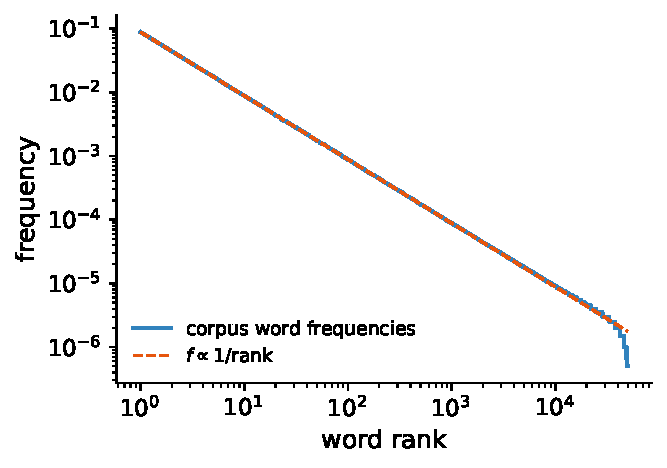
\includegraphics[width=0.55\linewidth]{fig/zipf.pdf}
  \caption{Zipf's law, illustrated on a synthetic corpus: $2\times10^6$ tokens drawn from a $1/k$ distribution over a vocabulary of $5\times10^4$ words, with the empirical rank--frequency curve against the $f\propto 1/\mathrm{rank}$ guide. The curve is a consistency check rather than data, since the words were sampled from a Zipf distribution to begin with. Real corpora look the same over roughly four decades, with deviations at both ends: the Zipf--Mandelbrot correction at low rank, and a steeper tail beyond about $10^4$ words.}
  \label{fig:zipf}
\end{figure}

The exponents of these tails differ, and the differences matter, because in every model below the loss exponent is inherited from the data exponent. Pure Zipf is in fact a marginal case. Write the tail of skill frequencies as $p_k\propto k^{-(\alpha+1)}$. The quantization model of Section \ref{sec:quanta} gives a loss exponent equal to $\alpha$, and exact Zipf ($f_k\propto 1/k$, that is, $\alpha = 0$) is the boundary at which the tail sum decays only logarithmically and power-law scaling degenerates. Read this way, the measured $\alpha_P\approx 0.076$ for language says that its effective skill distribution is $p_k\sim k^{-1.08}$, barely steeper than pure Zipf. Language scaling is slow because its structure sits just above the marginal $1/k$ tail. Image data has steeper tails and scales faster; compare the modality table of Section \ref{sec:scaling-empirical}.

Where does the theory stand? The single-resource laws have been derived from this mechanism by many models of quite different flavor, and a few models derive multi-resource laws; the survey below keeps score. Three things are missing. First, no theory computes the data's exponents from first principles. Every model converts measured data statistics into loss curves, and the statistics themselves are an empirical input. This is true even for procedurally generated math, where the generating program is known exactly but the computation has not been carried out. Second, there are no joint laws with genuine feature learning. The best dynamical derivations live in lazy, random-feature settings (Section \ref{sec:scaling-dmft}), while in solvable cases feature learning is known to improve exponents for structured targets, so the corrections need not be small. Third, the bridge from the smooth loss to capabilities is missing. Benchmark performance can jump within a decade of scale while the loss glides smoothly \cite{wei2022emergent}; this has been contested as an artifact of the metric \cite{schaeffer2023emergent}, and the quantization model of Section \ref{sec:emergence} gives it a sharper reading. A fourth gap is newer: the post-training and test-time scaling laws of Section \ref{sec:scaling-posttraining} have no theory at all.

\subsection{A survey of theoretical proposals}
\label{sec:scaling-survey}

The table below organizes the most prominent derivations of neural scaling laws by four questions: what models the \emph{data} (equivalently, what a ``feature'' is and how features are distributed); what models the \emph{network}, if anything; whether actual \emph{exponents} are predicted, and in terms of what; and whether \emph{multi-resource} laws are obtained.
%
\begin{center}
\footnotesize
\renewcommand{\arraystretch}{1.45}
\setlength{\tabcolsep}{3.5pt}
\begin{tabular}{>{\raggedright\arraybackslash}p{2.5cm}|>{\raggedright\arraybackslash}p{3.1cm}|>{\raggedright\arraybackslash}p{2.7cm}|>{\raggedright\arraybackslash}p{2.6cm}|>{\raggedright\arraybackslash}p{2.2cm}}
    \textbf{proposal} & \textbf{data model / ``features''} &
    \textbf{NN framework} & \textbf{exponents?} &
    \textbf{multi-resource?} \\\hline
    quantization; Michaud et al.\ \cite{michaud2023quantization} &
    discrete skill ``quanta,'' Zipf-used, learned in order & none (a
    counting argument) & in terms of the Zipf exponent $\alpha$; plus
    the relation $\tfrac{1}{\alpha_n} = \tfrac{1}{\alpha_P} + 1$ &
    separate $P$, $n$, $S$ laws \\
    data manifold; Sharma--Kaplan \cite{sharma2020neural} & smooth
    target on a $d$-dimensional manifold & piecewise-linear
    interpolation (function class only; no training) & yes: $\alpha_P \approx 4/d$ & no ($P$ only) \\
    percolation; Brill \cite{brill2024scaling} & latent subtask
    clusters at criticality, with power-law cluster sizes & none: a generic
    nonparametric learner $+$ regression estimates & from percolation critical
    exponents & two regimes; not joint \\
    kernel eigenlearning; Bahri et al.\ \cite{bahri2021explaining},
    Bordelon--Canatar--Pehlevan \cite{bordelon2020spectrum,canatar2021spectral,simon2023eigenlearning}
    & power-law kernel spectra $+$ target coefficients & \textbf{frozen kernel}:
    infinite-width NTK, or GP/Bayesian & in terms of the spectral exponents &
    partially: resolution- vs.\ variance-limited regimes \\
    solvable field theory; Maloney--Roberts--Sully
    \cite{maloney2022solvable} & latent power-law covariance, extended
    by random features & linear model on \textbf{fixed random features}
    (frozen kernel); large-$N$ RMT, statics & in terms of the data's spectral exponent & yes: joint
    $L(P,n)$, with duality $P \leftrightarrow n$ \\
    DMFT; Bordelon--Atanasov--Pehlevan \cite{bordelon2024dynamical} &
    power-law (source/capacity) spectra & DMFT of gradient-flow
    training on \textbf{fixed random features} (frozen kernel; dynamics) & yes, including the time exponent & fully
    joint $L(t,P,n)$ $+$ compute frontier \\
\end{tabular}
\end{center}

Five remarks for reading the table. First, everyone agrees on the origin. In every row the loss exponent is inherited from a power-law tail in the data, whether of skill frequencies, cluster sizes, manifold volume, or covariance spectra. The rows differ in what the tail is a tail \emph{of}, and in how much network machinery is retained. Second, and this deserves emphasis: \emph{every row that models the network at all does so with a frozen kernel}. The eigenlearning row works with the infinite-width NTK or GP kernel of Sections \ref{sec:NTK-const} and \ref{sec:Bayes-kernel}; the two field-theory rows train only the readout of a fixed set of random features, which is a frozen kernel by construction (\cref{ex:app-tangent}(b)). The manifold row models only the network's function class, as a count of linear pieces, and never trains it; the quantization and percolation rows contain no network. So none of the current derivations involves feature learning, the very mechanism that Sections \ref{sec:MFT}--\ref{sec:DMFT} argued is what makes finite networks differ from kernels. Third, equilibrium routes (Bayesian GP learning curves and their finite-width refinements) and dynamical routes (gradient flow, DMFT) give matching exponents wherever they overlap. This is the ``two limits of one system'' correspondence of Sections \ref{sec:Bayes} and \ref{sec:DMFT} at work again. Fourth, only the two field-theory rows currently predict joint laws, and only the dynamical one prices training time, deriving a Chinchilla-like compute-optimal frontier rather than assuming it. Fifth, no row computes the data's own exponent. The closest attempt is the percolation proposal, which derives power-law cluster-size statistics from a critical model of the data distribution; its two criticality regimes (power-law-distributed discrete subtasks, and a dominant data manifold) map onto the quantization and manifold rows respectively. We will not develop the percolation model further. The remaining subsections work through the other rows, in order of machinery.

\emph{Do the predicted exponents agree with experiment?} Where the comparison has been made, the answer is encouraging but not yet sharp. The quantization model's authors extracted ``quanta'' from a small language model by clustering gradients, measured how often each is used in the training distribution, and found a power law whose exponent roughly matches the model's scaling exponent, as the model requires \cite{michaud2023quantization}; on the other hand, the model's parameter-free relation between $\alpha_P$ and $\alpha_n$ is violated by the measured ordering of Kaplan's exponents (\cref{ex:quanta}(e)). The manifold prediction $\alpha_P\approx 4/d$ was confirmed in teacher--student experiments, where $d$ and $\alpha_P$ can be measured independently, and tested more loosely on image classifiers and GPT-type language models \cite{sharma2020neural}; for language, taking $\alpha_P\approx0.076$ at face value gives $d\approx 50$ (\cref{ex:manifold}). The kernel predictions have been tested on standard architectures and datasets, with exponents computed from measured kernel spectra, and the predicted duality between the $P$- and $n$-exponents holds up \cite{bahri2021explaining}. The two field-theory rows take the data's spectral exponent as input. Their qualitative predictions --- exponents independent of architecture, $\alpha_P\approx\alpha_n$, and equiparameterization as the compute-optimal rule --- match the Chinchilla-era measurements, but a quantitative test needs the covariance spectrum of the training data, which is rarely reported for the large runs.
%The percolation proposal has, as far as we know, not yet been compared quantitatively with measured exponents.
The honest summary is that these theories convert an exponent measured in the \emph{data} into an exponent measured in the \emph{loss}, and the conversion has held up wherever both have been measured.

\subsection{The quantization model: exponents from the statistics of skills}
\label{sec:quanta}

The quantization model of Michaud, Liu, Girit, and Tegmark \cite{michaud2023quantization} is a minimal model of scaling. It has no architecture, no optimizer, and essentially no mathematics beyond a tail sum, and it produces all three laws of \eqref{scaling-laws}, plus a sharp point of view on ``emergent capabilities.'' The name is deliberately provocative: the proposal is that what a network learns comes in \emph{discrete units}, dubbed \emph{quanta}.%
%
\footnote{Michaud's blog post \href{https://ericjmichaud.com/quanta/}{ericjmichaud.com/quanta} is an excellent companion to the paper and can substitute for it in this exercise. But attempt \cref{ex:quanta} \emph{before} reading either; the derivations are short, and they are more instructive to find than to follow.} %
%
The assumptions, in the form we'll use:
%
\begin{itemize}
    \item \textbf{QH1 (discreteness).} The computations and knowledge relevant to the prediction task decompose into enumerable \emph{quanta}: basic skills or facts (\emph{e.g.} ``carry the one,'' ``Paris follows `the capital of France is','' ...). Each quantum is either fully learned or not learned at all, with no partial credit.
    \item \textbf{QH2 (ordered acquisition).} Networks learn quanta roughly in order of decreasing usefulness, so a given model has learned the first $m$ quanta of a fixed sequence.
    \item \textbf{QH3 (Zipfian use).} Quantum $k$ is \emph{used} on a fraction
    %
    \begin{equation} \label{zipf}
        p_k = \frac{k^{-(\alpha+1)}}{\zeta(\alpha+1)}
    \end{equation}
    %
    of samples ($\alpha>0$ a constant), and on those samples, knowing it reduces the loss by a constant $\Delta$ (independent of $k$).
\end{itemize}
%
Consequently, a model that has learned the first $m$ quanta has expected loss
%
\begin{equation} \label{quanta-loss}
    L_m = L_\infty + \Delta \sum_{k>m} p_k\,.
\end{equation}
%
That is the entire model. Everything else is asking how $m$ is limited by each resource.

\begin{exercise}[Three scaling laws from three assumptions]
\label{ex:quanta}
\important
\begin{enumerate}
    \item Estimate the tail sum in \eqref{quanta-loss} to show $L_m - L_\infty \propto m^{-\alpha}$.
    \item \emph{Parameter-limited (data and training unlimited).} Suppose each quantum costs a constant capacity of $c$ parameters to learn. Derive $\alpha_P$ in terms of $\alpha$.
    \item \emph{Data-limited (capacity and training unlimited).} Suppose a quantum is learnable only if it is used by at least $\tau$ training samples, for constant $\tau$. Given $n$ i.i.d.\ samples, which quanta are learnable? Derive $\alpha_n$.
    \item \emph{Training-limited, single epoch.} Suppose instead that learning quantum $k$ requires $\tau$ gradient updates on batches containing it. After $S$ steps of online training (fresh batches), derive $\alpha_S$.
    \item \emph{Falsifiability.} Parts (b)--(c) predict a parameter-free relation between $\alpha_P$ and $\alpha_n$: write it down, and note which of the two exponents must be larger. Compare with the measured values quoted after \eqref{scaling-laws}. Something is wrong --- what? List the assumptions you used and discuss which are most suspect. (This is a discussion question with no settled answer; see the solution for candidates.)
\end{enumerate}
\end{exercise}


\subsection{Emergence: smooth laws from staggered cliffs}
\label{sec:emergence}

The quantization model's deepest payoff is conceptual. Under QH1, the learning of any \emph{single} quantum is a step function: a capability is absent, then abruptly present. Yet the aggregate loss \eqref{quanta-loss} is a smooth power law. There is no contradiction. \emph{A smooth law is a sum of many staggered cliffs}, each weighted by $p_k$ and individually invisible in the aggregate, since quantum $k$ contributes only the small fraction $p_k$ of the loss. Michaud et al.\ sharpen this with a genetics metaphor. A test sample is \emph{monogenic} if its loss is governed by a single quantum, so that its loss curve during training is a plateau followed by a cliff; it is \emph{polygenic} if many quanta contribute, in which case its loss falls smoothly. Both kinds of per-token curves are observed in real LLMs. From this perspective, ``emergent capabilities'' \cite{wei2022emergent} are neither magic nor mirage \cite{schaeffer2023emergent}: any benchmark dominated by a few quanta \emph{must} show abrupt arrival, while any sufficiently aggregated metric \emph{must} look smooth. Emergence is a property of what you measure, not (necessarily) of a phase transition inside the model.

\begin{figure}[ht]
  \centering
  \includegraphics[width=0.98\linewidth]{fig/sparse-parity.pdf}
  \caption{Multitask sparse parity \cite{michaud2023quantization}: smooth scaling from staggered cliffs. Setup: $T=48$ subtasks with Zipfian frequencies $p_i \propto i^{-(\alpha+1)}$, $\alpha=0.4$; inputs are a one-hot task indicator ($T$ bits) concatenated with $24$ random $\pm1$ bits; the label is the parity of a fixed random $3$-subset of the bits, the subset depending on the task. Model: one-hidden-layer ReLU MLP, width $512$, MSE loss on $\pm1$ labels, trained online (fresh batches of $256$; Adam, learning rate $2\times10^{-3}$, $1.2\times10^5$ steps; fixed seed). \emph{Left:} test loss per subtask vs.\ training step. Each subtask is learned in an abrupt cliff, frequent tasks first. \emph{Right:} the frequency-weighted aggregate $L(S)=\sum_i p_i L_i(S)$ is smooth; the dashed guide is the \emph{idealized} quanta-model slope $-\alpha/(\alpha+1)$ from \cref{ex:quanta}(d). The measured decay is visibly steeper, as discussed in the text.}
  \label{fig:sparse-parity}
\end{figure}

\textbf{Lab: multitask sparse parity.} The entire mechanism fits in a laptop-scale experiment, shown in \cref{fig:sparse-parity}; students are encouraged to reproduce and modify it (all details are in the caption). A network is trained online on $T$ separate parity subtasks with Zipfian frequencies. The input is a one-hot task indicator concatenated with random bits, and the label is the parity of a small task-specific subset of the bits. Parity is a needle-in-a-haystack skill with no partial credit, \emph{i.e.} an honest hand-built quantum. The result: each subtask's test loss is a staggered cliff (frequent tasks fall first), while the frequency-weighted aggregate loss decays smoothly. Note also the honest failure visible in the right panel. The measured aggregate decays \emph{more steeply} than the idealized quanta slope $-\alpha/(\alpha+1)$ of \cref{ex:quanta}(d), because the cliffs bunch up rather than spreading Zipf-like; the rare tasks are learned sooner than the threshold rule $S\,p_k\gtrsim\tau$ predicts. The subtasks share a hidden layer and an adaptive optimizer, so they are not learned independently, and assumption (iv) in the solution to \cref{ex:quanta}(e) fails.

\subsection{Exponents from geometry and from spectra}
\label{sec:eigenlearning}

The quantization model takes the Zipf exponent $\alpha$ as \emph{input}. The next two arguments produce exponents as \emph{output}, from properties of the data.

\subsubsection{Geometry: the data-manifold argument}

Sharma and Kaplan \cite{sharma2020neural} propose the simplest continuous mechanism. A network with ReLU activations computes a piecewise-linear function, so regression on a data manifold of intrinsic dimension $d$ is a problem of \emph{piecewise-linear interpolation}. A network with $P$ parameters can afford $\sim P$ linear pieces; tiling a $d$-dimensional manifold with $P$ pieces gives spacing $s \sim P^{-1/d}$; a linear patch approximates a smooth target to accuracy $\sim s^2$ (Taylor); and MSE is the \emph{square} of the error. Hence
%
\begin{equation} \label{manifold-law}
    L(P) \sim (s^2)^2 \sim P^{-4/d}\,,\qquad \alpha_P \approx \frac{4}{d}\,.
\end{equation}
%
Exponents are small because data manifolds are high-dimensional. The formula is testable, since $d$ can be measured with intrinsic-dimension estimators, which is exactly what \cite{sharma2020neural} do.

\begin{exercise}[Exponents from the data manifold]
\label{ex:manifold}
(a) Fill in the derivation of \eqref{manifold-law}, stating precisely where smoothness of the target is used. (b) How does the answer change for mean-absolute-error loss? (c) Taking the measured $\alpha_P\approx0.076$ for language models at face value, estimate the effective dimension of the ``manifold of text.'' Discuss whether the input dimension, the embedding dimension, or something else is being measured. (d) What does this mechanism predict for the \emph{data} exponent $\alpha_n$, if $n$ samples are what limits the resolution of the tiling?
\end{exercise}


\subsubsection{Spectra: scaling laws from kernel eigenvalues}

The second mechanism uses machinery we already own: the Bayesian kernel regression of Section \ref{sec:Bayes-kernel}, whose mode-filtering formula said that with $n$ samples (and inverse temperature $\beta$), the modes of the GP kernel that get learned are those with $\lambda_k \gtrsim (n\beta)^{-1}$. Suppose the kernel spectrum and the target's decomposition are power laws,
%
\begin{equation}
    \lambda_k \sim k^{-a}\quad (a>1)\,,\qquad y_k^2 \sim k^{-b}\quad (b>1)\,,
\end{equation}
%
in a shared eigenbasis $\{\varphi_k\}$. The unlearned modes dominate the test error:
%
\begin{equation} \label{spectral-law}
    L(n) \;\sim\; \sum_{k \,:\, \lambda_k \lesssim (n\beta)^{-1}} y_k^2
    \;\sim\; \sum_{k > k_*} k^{-b}
    \;\sim\; k_*^{\,1-b}\,,\qquad k_* \sim (n\beta)^{1/a}\,,
\end{equation}
%
giving $L(n) \sim n^{-(b-1)/a}$: \emph{the scaling exponent is a ratio of spectral decay rates}. Everything about the data and the architecture enters through two measurable power laws. This is the starting point of the ``eigenlearning'' analyses \cite{bordelon2020spectrum,canatar2021spectral,simon2023eigenlearning}, which sharpen \eqref{spectral-law} into precise learning curves (including the overfitting factor whose divergence produces the double-descent peak of Section \ref{sec:DMFT}). Bahri et al.\ \cite{bahri2021explaining} organize the possibilities into a clean $2\times2$ taxonomy: \emph{resolution-limited} regimes (exponents from spectra or geometry, as here and in \eqref{manifold-law}) versus \emph{variance-limited} regimes (universal exponent $1$), in each of $P$ and $n$.

\begin{exercise}[Spectral scaling laws, and quanta as eigenmodes]
\label{ex:spectra}
(a) Derive \eqref{spectral-law} from the mode-filtering formula of Section \ref{sec:Bayes-kernel}, and check that the crossover modes $k\sim k_*$ do not change the exponent.
(b) Show that the quantization model's data-scaling law is the special case $b=a$ of \eqref{spectral-law} under the dictionary: quanta $=$ eigenmodes, Zipf law $=$ spectrum, $a = \alpha+1$. (Hint: in the quanta model, $p_k$ plays \emph{both} roles, setting the learning threshold \emph{and} the contribution $\Delta\,p_k$ to the loss, so the two power laws coincide.)
(c) In the quanta model, what would it mean for $b \neq a$? Invent a modification of QH3 that realizes it.
\end{exercise}


\subsection{A solvable large-N field theory}
\label{sec:MRS}

Maloney, Roberts, and Sully \cite{maloney2022solvable} supply what the arguments above lack: a \emph{microscopic, exactly solvable} model in which the joint law $L(P,n)$ is computed, not modeled. The ingredients are: a generative data model in which observed inputs are (nonlinear functions of) random projections of a latent space, engineered so that the data covariance has a power-law spectrum $\lambda_k \sim k^{-(1+\zeta)}$, as measured in real image and text data (the spectral exponent is the paper's $\gamma$; we reserve $\gamma$ for the scaling dial of Section \ref{sec:MFT-dial}); a random-feature \emph{linear} student, so we are in the lazy limit of Section \ref{sec:train}, whose $P$ random features are its trainable parameters, trained on $n$ samples; and the joint thermodynamic limit $P,n\to\infty$ at fixed ratio. The computation proceeds at large $P$ and $n$, where expectations over data and features become Gaussian integrals, the test loss becomes a product of resolvents (Green's functions), and the $1/P$ expansion organizes into planar ('t Hooft) diagrams that can be resummed exactly.%
%
\footnote{This is also a working example for Section \ref{sec:DMFT}'s toolkit: the same model can be solved dynamically, and its double-descent peak, at the interpolation threshold $P\sim n$, is regularized by ridge or early stopping, connecting back to the divergence of the overfitting factor mentioned in Section \ref{sec:eigenlearning}.}

\emph{Frozen, but random.} A natural first reaction is that this model should be trivial. The student is a linear model on fixed random features. Its kernel never moves, so we are squarely in the lazy regime of Section \ref{sec:train}, and in the strict infinite-width lazy limit the loss would not depend on $P$ at all. The $P$-scaling law is a \emph{finite-size effect on the lazy limit}. At finite $P$ the feature Gram matrix is a \emph{random} matrix, correlated with the random sample, and its rank caps how many modes of the data spectrum the student can resolve. All of the physics lives in the disorder average over this randomness, which is what the resolvents and the planar diagrams compute. Frozen does not mean deterministic.

Three notable results:
%
\begin{itemize}
    \item \emph{Where exponents come from:} the loss inherits the \emph{data's} spectral exponent, $L \sim \min(P,n)^{-\zeta}$ up to logarithms. Remarkably, generic nonlinear feature maps \emph{extend} the data's power-law spectrum rather than reshaping it. This explains why exponents are roughly architecture-independent and can only be improved by changing the data (or the task).
    \item \emph{Duality and Chinchilla:} the loss is (to leading order) \emph{symmetric} under $P\leftrightarrow n$. This predicts $\alpha_P \approx \alpha_n$, consistent with observation, and opposite in spirit to the quanta model's asymmetric prediction (\cref{ex:quanta}(e)). It makes \emph{equiparameterization} $P\propto n$ compute-optimal, a first-principles Chinchilla rule.
    \item \emph{Where laws break:} scaling stops when $\min(P,n)$ exceeds the latent dimensionality of the data model, and the loss plateaus. Power laws are a statement about the resolvable structure in the data, and they end when the structure is exhausted.
\end{itemize}

\subsection{All the knobs at once: a dynamical theory}
\label{sec:scaling-dmft}

Everything so far is statics, or one knob at a time. The current frontier is the \emph{dynamical} mean-field theory of Section \ref{sec:DMFT} applied to scaling. Bordelon, Atanasov, and Pehlevan \cite{bordelon2024dynamical} solve a random-feature model trained by gradient flow, with power-law data spectra, in the joint limit of large width, large data, and long time. They obtain a single self-consistent prediction for $L(t, P, n)$, with the correlation and response functions of Section \ref{sec:DMFT} as the order parameters. Each resource, when it is the binding constraint, contributes its own power law, recovering the resolution-limited exponents of Section \ref{sec:eigenlearning} in the appropriate corners. Moreover, the theory predicts the full \emph{compute-optimal frontier}: minimizing $L$ at fixed compute $C \propto P t$ yields Chinchilla-like allocation rules and the frontier exponent, rather than assuming them.

A fair question: the features here are again frozen and random, exactly the setting of Section \ref{sec:MRS}, so is dynamical mean-field theory overkill? No, for two reasons. First, time is a genuine third resource. Predicting $L(t,P,n)$ and the compute frontier requires the whole training trajectory, and the statics only sees the $t\to\infty$ corner. Second, the naive mode-by-mode solution of the lazy regime, in which each kernel eigenmode of the residual decays as $e^{-\eta\lambda_k t}$ as in \eqref{exp-const}, applies to a \emph{deterministic} kernel. Here the kernel's eigenvalues and eigenvectors are random and correlated with the sampled data, so the disorder average couples the modes. The DMFT correlation and response functions are the dynamical generalization of the static resolvents of Section \ref{sec:MRS}, and at $t\to\infty$ the equations collapse back onto the static answer, as they must. What the theory is \emph{not} yet doing is feature learning. The adaptive-kernel version of the formalism exists \cite{bordelon2022self}, but it has not been pushed through power-law data to closed-form scaling laws; these are the ``joint laws with genuine feature learning'' missing from Section \ref{sec:scaling-origins}. Since feature learning is known to improve exponents for structured targets in solvable cases, the correction need not be small.

\subsection{Beyond pretraining: post-training and test-time scaling}
\label{sec:scaling-posttraining}

Frontier models are no longer just pretrained. They are fine-tuned on curated demonstrations (SFT), optimized against reward models or verifiable rewards (RLHF, RLVR), and allowed to spend variable compute at inference time. Do scaling laws extend to these stages? Increasingly, yes. But the functional forms change, and the changes are instructive.

\emph{Transfer and fine-tuning} still look Kaplan-like. The value of pretraining for a downstream task can be quantified as the \emph{effective data transferred}, meaning the amount of fine-tuning data that the pretrained initialization is worth, and it scales as a power law in both the fine-tuning dataset size and the model size \cite{hernandez2021transfer}.

\emph{Reward-model optimization} introduces a new scaling axis: not data or parameters, but the distance moved from the base policy, $d = \sqrt{\mathrm{KL}(\pi \,\|\, \pi_0)}$. Gao, Schulman, and Hilton \cite{gao2023reward} found that the true (``gold'') reward follows simple laws in $d$, namely $d\,(a - b\log d)$ for best-of-$n$ sampling and $d\,(a - b\,d)$ for RL, with coefficients that scale smoothly with the size of the reward model. Note the shape: not a power law but a rise and a \emph{fall}. Optimizing a learned proxy eventually degrades the true objective. This is a Goodhart peak, quantified.

\emph{RL on verifiable rewards}, the training recipe of the reasoning models, scales by \emph{saturating sigmoids} rather than power laws. In the largest systematic study to date, performance as a function of RL compute is predictable, but by a fit with an asymptote, an efficiency, and a midpoint, and most recipe choices move the efficiency without changing the asymptote \cite{khatri2025art}. A physics gloss suggests why the form differs, though it is a hypothesis rather than a result. Pretraining mines an effectively unbounded Zipf tail of new structure, hence power laws. RL post-training mostly elicits and reweights capabilities the base model already contains, on a bounded task distribution. In quanta language, pretraining acquires quanta, while RL sharpens the policy over quanta it already has, and one runs out. \emph{Test-time compute} is the other new axis: the coverage achieved by repeated sampling grows roughly as a power law in the number of samples \cite{brown2024monkeys}, and train-time and test-time compute can be traded against each other along a compute-optimal frontier \cite{snell2024test}.

What does not yet exist is a joint law over all four budgets (pretraining, SFT, RL, inference), and any \emph{theory} at all, even at the level of the quantization model, that derives the sigmoid or the Goodhart peak from a model of the data and skill distribution. The empirical forms are waiting for a statistical-mechanics treatment.

That every ingredient of the pretraining synthesis --- Gibbs measures, kernels, mean-field limits, MSRJD actions --- appeared earlier in these notes as a physics import is, we hope, a fair summary of the state of the field. A theory of the scaling laws is not finished, but it is recognizably being built, and it is being built out of statistical physics. The post-training laws are younger still: their regularities are only now being settled, and there is no theory of them yet. For a student entering the field, that is a map of where the open territory begins.





%===============================================================================
\appendix
% cleveref does not pick up \appendix on its own here, so tell it that section-level
% labels from this point on are appendices (\cref then prints "Appendix A.3").
\crefalias{section}{appendix}
\crefalias{subsection}{subappendix}
\crefalias{subsubsection}{subsubappendix}

\section{The replica method}
\label{app:replica}

Section \ref{sec:dictionary} introduced the quenched free energy $-\E_{\rm data}\log Z$ and the annealed approximation \eqref{annealed-swap} that replaces it by $-\log\E_{\rm data}Z$, and Section \ref{sec:ising} used that approximation to analyze the Ising perceptron. This appendix explains how the quenched average is computed exactly, by the \emph{replica method}, and what the annealed approximation misses. We keep the Ising perceptron of Section \ref{sec:ising} as the running example, in the notation and normalization of that section: $N$ binary weights $\theta\in\{\pm1\}^N$, a binary teacher $\theta^*$, Gaussian inputs, $n=\alpha N$ examples, and the partition function \eqref{perc-Z}. The classic reference for everything here is Engel and Van den Broeck \cite{engel2001statistical}.

\subsection{What the annealed approximation gets wrong}
\label{app:annealed-correction}

Jensen's inequality gives $\log\E Z\geq\E\log Z$, so the annealed free energy $-\log\E Z$ is always a lower bound on the quenched one. To see what drives the gap, write $Z = e^{-N\varphi}$, where the free-energy density $\varphi$ fluctuates from dataset to dataset. Exponentiation turns modest fluctuations of $\varphi$ into enormous fluctuations of $Z$: a dataset whose $\varphi$ is below the typical value by a constant is exponentially rare, but it contributes an exponentially large $Z$, and the two exponentials compete at the same order in $N$. The average $\E Z$ can therefore be dominated by vanishingly rare datasets, while the typical dataset, which is what $\E\log Z$ describes, behaves differently. (This is the familiar behavior of lognormal random variables, whose mean sits far in the upper tail. The mean is a poor summary of a heavy-tailed quantity.)

For the Ising perceptron the direction of the error follows. The datasets that dominate $\E Z$ are those that constrain the student unusually weakly, and weakly constrained students sit at low overlap. The annealed average therefore overweights poorly aligned students, and overestimates the amount of data needed to learn: it puts the transition to perfect generalization at $\alpha_c^{\rm ann}\approx1.45$, where the exact calculation sketched below gives $\alpha_c\approx1.245$ \cite{gyorgyi1990first}. The structure of the transition, two basins exchanging dominance, is the same in both.

\smallskip
\textbf{Remark:} Annealing does not always err so gently. Here the model is realizable (a teacher exists) and the fluctuations of $\varphi$ are tame, so annealing shifts a number without changing the picture. In general the annealed computation can fail qualitatively, most famously for models with discrete weights at large load, where it can predict negative entropies (fewer than one consistent student, nonsense for a count) and spurious transition points.

\subsection{Replicas}
\label{app:replica-method}

The full calculation computes $\E_{\rm data}\log Z$ through the identity
%
\begin{equation}
    \E\log Z = \lim_{Q\to0}\frac{\E Z^Q - 1}{Q}\qquad\big(\text{from } Z^Q = e^{Q\log Z} = 1 + Q\log Z + O(Q^2)\big)\,. \label{replica-identity}
\end{equation}
%
The strategy is to compute $\E Z^Q$ for \emph{integer} $Q$, where it has a transparent meaning, obtain a formula analytic in $Q$, and continue it to $Q\to0$. For integer $Q$, $Z^Q$ is the partition function of $Q$ independent copies, or \emph{replicas}, of the student, all judged against the same dataset. For the Ising perceptron, from \eqref{perc-Z},
%
\begin{equation}
    \E Z^Q = \frac{1}{2^{NQ}}\sum_{\theta^1,\ldots,\theta^Q\in\{\pm1\}^N}\;\E_{\rm data}\prod_{\mu=1}^n\prod_{a=1}^Q\Theta\big(y^\mu\,(\theta^a\cdot x^\mu)\big)\,. \label{EZn}
\end{equation}
%
The data average is easy, because the inputs are Gaussian. For fixed replicas and teacher, each example enters only through the $Q+1$ numbers $u^a = \theta^a\cdot x^\mu/\sqrt N$ and $v = \theta^*\cdot x^\mu/\sqrt N$, which are exactly jointly Gaussian (they are linear in $x^\mu$), with mean zero and a covariance determined entirely by the \emph{overlap matrix}
%
\begin{equation}
    q^{ab} = \frac{\theta^a\cdot\theta^b}{N}\,,\qquad R^a = \frac{\theta^a\cdot\theta^*}{N}\,:\qquad
    \E[u^au^b] = q^{ab}\,,\quad \E[u^av] = R^a\,,\quad \E[v^2] = 1\,. \label{overlap-matrix}
\end{equation}
%
The product of step functions asks that every $u^a$ have the sign of $v$, and the probability of that event is some function $e^{-e(q,R)}$ of the overlaps alone: a Gaussian orthant probability in $Q+1$ dimensions. Since the examples are independent, the data average of the product over $\mu$ is the $n$-th power, $e^{-n\,e(q,R)} = e^{-\alpha N\,e(q,R)}$. For $Q=1$ the only overlap is $R$, the orthant is a wedge, and $e(R) = -\log(1-\varepsilon(R))$ is the energy term of Section \ref{sec:ising}.

The disorder is gone. In its place, the replicas are coupled through the overlaps $q^{ab}$, and the sum over the $Q$ binary vectors can be organized by the value of the overlaps, exactly as the sum over one binary vector was organized by $R$ in \cref{ex:ising}(c). Writing $e^{N\,h(q,R)}$ for the number of $Q$-tuples of students with prescribed overlaps (for $Q=1$ this is the binomial count of \cref{ex:ising}(c)), and replacing the sum over overlaps by an integral,
%
\begin{equation}
    \E Z^Q \;\approx\; \int dq\,dR\; e^{-N\,s_Q(q,R)}\,,\qquad s_Q(q,R) := Q\log 2 - h(q,R) + \alpha\,e(q,R)\,. \label{replica-action}
\end{equation}
%
This is the replicated version of the one-variable action \eqref{perc-action} of Section \ref{sec:ising}, to which it reduces at $Q=1$. At large $N$ the integral is dominated by the minimum of $s_Q$ over the overlaps, and the replica identity \eqref{replica-identity} then gives the quenched free-energy density
%
\begin{equation}
    \Phi(\alpha) := -\frac{1}{N}\,\E_{\rm data}\log Z \;=\; \lim_{Q\to0}\;\frac{1}{Q}\,\min_{q,R}\,s_Q(q,R)\,. \label{replica-saddle}
\end{equation}
%
Compare the annealed approximation, which is $\min_R s_1(R)$: the annealed calculation keeps a \emph{single} replica, and so never sees the coupling $q^{ab}$ between replicas that the shared data induce. That coupling is precisely the information about dataset-to-dataset fluctuations that Section \ref{app:annealed-correction} found missing.

\emph{Replica symmetry.} To make \eqref{replica-saddle} concrete one needs $h$ and $e$ as functions of the $Q(Q+1)/2$ overlaps, and a way to continue the result in $Q$. The standard ansatz, \emph{replica symmetry}, is to take $q^{ab} = q$ for all $a\neq b$ and $R^a = R$. It is natural, since the saddle-point equations are symmetric under permuting replicas, and it reduces the problem to two scalars. Under it, both $h$ and $e$ become one-dimensional Gaussian integrals: the orthant probability collapses to an integral over a single shared Gaussian ``field'' of the Gaussian tail function $H(x) = \int_x^\infty\frac{dz}{\sqrt{2\pi}}e^{-z^2/2}$, and the count $h$ is handled by introducing conjugate variables for the constraints, which reduces it to a one-site problem in the manner of the mean-field Ising model of Section \ref{sec:ising-model}. The resulting expression is analytic in $Q$ and can be differentiated at $Q=0$. As a caution, symmetric equations \emph{can} have asymmetric solutions, and this happens in physical systems, famously in spin glasses; the assumption must be checked, and for the perceptron problems considered here it holds.

\emph{The result.} For the Ising perceptron, the replica-symmetric calculation \cite{gyorgyi1990first} reproduces the two-basin structure found in \cref{ex:ising}: an interior solution with $R^*(\alpha)<1$ that drifts toward the teacher as data accumulate, and the teacher solution $R=1$, which exchange dominance in a first-order transition. Only the number moves, from $\alpha_c^{\rm ann}\approx1.45$ to $\alpha_c\approx1.245$. A guided walk through the calculation follows.

\begin{exercise}[The quenched calculation, via replicas]
\label{ex:replica}
Work through the following program for the Ising perceptron, in as much detail as your appetite allows; full details are in \cite[chs.~2 and 7]{engel2001statistical}.
\begin{enumerate}
    \item \emph{Replicate.} For integer $Q$, write $\E Z^Q$ as in \eqref{EZn}: a $Q$-fold copy of the system, coupled only through the shared data.
    \item \emph{Average over data.} Show that for fixed replicas and teacher, $u^a = \theta^a\cdot x/\sqrt N$ and $v = \theta^*\cdot x/\sqrt N$ are exactly jointly Gaussian with the covariance \eqref{overlap-matrix}, and that the data average factorizes across examples, each contributing the same function $e^{-e(q,R)}$ of the overlaps. Check that at $Q=1$, $e(R) = -\log(1-\varepsilon(R))$ with $\varepsilon$ the wedge formula \eqref{eps-of-R}.
    \item \emph{Push forward to the order parameters.} Insert delta functions fixing $q^{ab}$ and $R^a$ (in integral representation, with conjugate variables $\hat q^{ab}$, $\hat R^a$), so that the sum over the binary vectors factorizes over sites $i=1,\ldots,N$ and becomes the $N$-th power of a $Q$-spin sum. Conclude that $\E Z^Q$ takes the form \eqref{replica-action}, and that the annealed action \eqref{perc-action} is its $Q=1$ case.
    \item \emph{Replica symmetry.} Take $q^{ab} = q$ for $a\neq b$ and $R^a = R$ (and likewise for the conjugates). Show that the orthant probability becomes $e^{-e_{\rm RS}} = 2\int Dt\,H(\cdot)^Q$ for an appropriate argument of the tail function $H$, built from $q$, $R$, and a single Gaussian variable $t$, and that the site sum becomes a one-dimensional Gaussian integral of $(2\cosh(\cdot))^Q$. Continue both in $Q$ and expand to first order at $Q=0$.
    \item \emph{Use the symmetry of Gibbs learning.} A student drawn uniformly from the consistent set is statistically indistinguishable from the teacher, since the teacher is itself a uniformly random binary vector consistent with the data. Argue that this forces $q = R$ at the saddle: the overlap between two Gibbs students equals their overlap with the teacher. One scalar remains, with one conjugate.
    \item \emph{Solve.} The saddle-point equations for $R(\alpha)$ are transcendental. Solve them numerically and show that there are two competing solutions, an interior one and $R=1$, whose free energies cross at $\alpha_c\approx1.245$. Compare with the annealed $\alpha_c^{\rm ann}\approx1.45$ of \cref{ex:ising}(g), and explain the direction of the shift using Section \ref{app:annealed-correction}.
\end{enumerate}
\end{exercise}

\subsection{A variant: the spherical perceptron}
\label{app:sph-perceptron}

The replica method is easiest to push all the way to closed form in a variant of the problem with \emph{continuous} weights, which is also the classic case in which the annealed and quenched learning curves can be compared analytically. Keep everything in Section \ref{sec:ising} the same, but let the weights be real, $\theta,\theta^*\in\R^N$. Since $f_\theta = \mathrm{sign}(\theta\cdot x)$ is invariant under $\theta\to\lambda\theta$ with $\lambda>0$, remove the redundant scale by putting the weights on a sphere,
%
\begin{equation}
    |\theta|^2 = |\theta^*|^2 = N\,, \label{sph-constraint}
\end{equation}
%
normalized so that individual weights stay of order one, and let the prior be the uniform measure $\pi(\theta)\,d\theta$ on the sphere. This is the \emph{spherical perceptron}. The wedge formula \eqref{eps-of-R} for the generalization error is unchanged, since its derivation used only that $(\theta\cdot x,\theta^*\cdot x)/\sqrt N$ is a Gaussian pair with correlation $R$, which holds for any $\theta$ with $|\theta|^2 = N$. What changes is the entropy: the number of students at overlap $R$ becomes the \emph{volume} of the slice of the sphere at overlap $R$. Decompose $\theta = R\,\theta^* + \theta_\perp$ with $\theta_\perp\perp\theta^*$. The constraint \eqref{sph-constraint} gives $|\theta_\perp|^2 = N(1-R^2)$, so the slice is a sphere of radius $\sqrt{N(1-R^2)}$ in the $(N-1)$-dimensional orthogonal complement, of volume $\propto\big(N(1-R^2)\big)^{(N-2)/2}$, and
%
\begin{equation}
    \frac{1}{N}\log\int_{\theta:\,R(\theta)=R}d\theta\,\pi(\theta) \;=\; h(R) = \tfrac{1}{2}\log(1-R^2) + \text{const} + O\big(\tfrac{1}{N}\log N\big)\,. \label{coarea}
\end{equation}
%
Repeating the annealed calculation of \cref{ex:ising}(d) with this entropy gives
%
\begin{equation}
    \E_{\rm data}Z \approx \int_{-1}^1 dR\; e^{-N\,S_{\rm ann}(R)}\,,\qquad
    S_{\rm ann}(R) := \underbrace{-\tfrac{1}{2}\log(1-R^2)}_{\text{entropy}}\;\underbrace{-\;\alpha\log\big(1-\varepsilon(R)\big)}_{\text{energy}}\,, \label{annealed-integral}
\end{equation}
%
and the annealed free-energy density is
%
\begin{equation}
    \Phi_{\rm ann}(\alpha) := \min_R S_{\rm ann}(R)\,. \label{annealed-saddle}
\end{equation}

\Cref{fig:gann} shows $S_{\rm ann}$ for several loads. The entropy--energy competition is the same as for the Ising perceptron, but the outcome is different: the entropy $-\frac{1}{2}\log(1-R^2)$ diverges as $R\to1$, so the perfectly aligned state is infinitely penalized, the minimum always sits in the interior, and it slides continuously from $R=0$ toward $R=1$ as $\alpha$ grows. There is no phase transition. This is the answer to the closing question of \cref{ex:ising}(h): the binary weights of the Ising perceptron give the aligned state finite entropy, $h(1)=0$, and that is what allows it to compete as a separate basin.

\begin{figure}[ht]
  \centering
  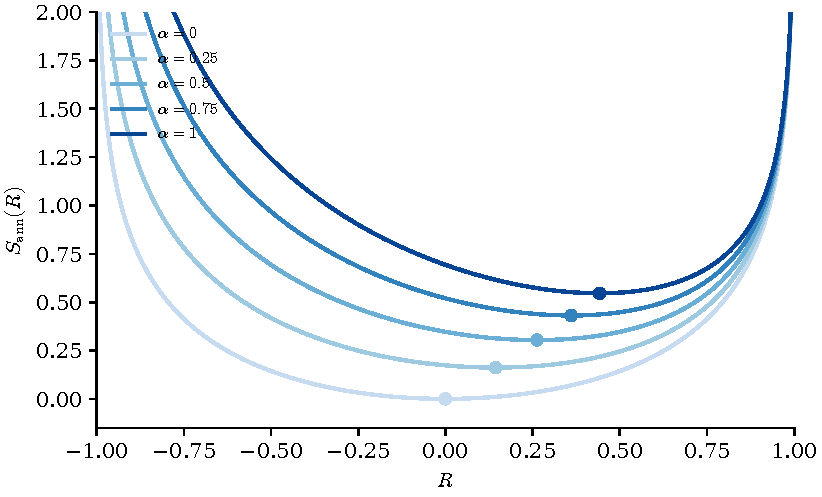
\includegraphics[width=0.62\linewidth]{fig/spherical-action.pdf}
  \caption{The annealed action $S_{\rm ann}(R)$ of the spherical perceptron, \eqref{annealed-integral}, for $\alpha\in\{0,0.25,0.5,0.75,1\}$ (bottom to top at $R=0$), with the minimizer marked on each curve. The entropy pins the minimum at $R=0$ when $\alpha=0$; increasing the load slides it smoothly toward larger overlap, and the entropic wall at $R=1$ keeps it in the interior. One basin at every $\alpha$, moving continuously: no phase transition.}
  \label{fig:gann}
\end{figure}

\emph{The learning curve.} The large-$\alpha$ behavior follows by expanding near $R=1$. Writing $R = \cos(\pi\varepsilon)$, so that $\varepsilon$ is the generalization error itself, $1-R^2\approx(\pi\varepsilon)^2$ and
%
\begin{equation}
    S_{\rm ann}\approx -\log(\pi\varepsilon) + \alpha\,\varepsilon + \text{const}\,, \label{Gann-large-alpha}
\end{equation}
%
which is minimized at
%
\begin{equation}
    \varepsilon_{\rm ann}(\alpha) \simeq \frac{1}{\alpha}\,. \label{annealed-eps}
\end{equation}
%
The generalization error decays as a \emph{power law} in the amount of data, with exponent one: the simplest instance of the scaling laws of Section \ref{sec:scaling}. The exact, quenched treatment \cite{seung1992statistical,engel2001statistical} runs through the replica steps of \cref{ex:replica} with the volume entropy \eqref{coarea} in place of the count (here replica symmetry can be justified by the convexity of the region of the sphere consistent with the data), and yields
%
\begin{equation}
    \varepsilon_{\rm Gibbs}(\alpha)\simeq\frac{0.625}{\alpha}\,: \label{quenched-eps}
\end{equation}
%
the same exponent, with a different constant. As in Section \ref{app:annealed-correction}, the annealed average overweights poorly aligned students and overestimates the error, $1/\alpha>0.625/\alpha$; and since the model is realizable, the exponent survives the approximation even though the constant does not.

\begin{exercise}[The annealed learning curve of the spherical perceptron]
\label{ex:annealed}
(a) Derive the slice entropy \eqref{coarea}, and assemble the annealed action \eqref{annealed-integral} by repeating the steps of \cref{ex:ising}(d).
(b) Derive the saddle-point condition for \eqref{annealed-saddle}, and show that $R=1$ is never a minimum, in contrast with \cref{ex:ising}(f).
(c) Verify the large-$\alpha$ learning curve \eqref{annealed-eps}, and show that at small $\alpha$ the annealed theory predicts $R\propto\alpha$. Sketch the full learning curve $\varepsilon(\alpha)$.
(d) Which steps of \cref{ex:replica} change when the count of binary students is replaced by the volume \eqref{coarea}, and which do not?
\end{exercise}

%===============================================================================
\section{From linear regression to kernel regression}
\label{app:kernels}

This appendix is a self-contained review of models that are \emph{linear in their parameters}: linear regression, regression on fixed nonlinear features, kernel regression, and kernel \emph{ridge} regression. It ends with the observation that a neural network linearized around its initialization --- the ansatz \eqref{f-lin} of Section \ref{sec:train} --- is exactly such a model, so that training it amounts to kernel ridge regression. Nothing here requires large width, gradient-flow asymptotics, or moving features; those are the subjects of Sections \ref{sec:init}--\ref{sec:MFT}, and this appendix supplies the linear algebra they rest on. Readers who found the kernel formulas of Sections \ref{sec:NTK} and \ref{sec:Bayes-kernel} appearing out of thin air may want to read it first.%
\footnote{This appendix adapts a lecture and an exercise notebook prepared by Charles Renshaw-Whitman for the Iliad Intensive, translated into the notation of Section \ref{sec:setup}.}

We use the notation of Section \ref{sec:setup}: training data $(x^\mu,y^\mu)_{\mu=1}^n$ with $x^\mu\in \R^d$ and $y^\mu\in\R$; a model $f_\theta:\R^d\to \R$ with parameters $\theta\in \R^P$; and $f^\mu := f_\theta(x^\mu)$ for its values on the training inputs. It is convenient to stack the data into matrices,
%
\begin{equation}
    X := \begin{pmatrix} (x^1)^T \\ \vdots \\ (x^n)^T \end{pmatrix} \in \R^{n\times d}\,,\qquad
    Y := \begin{pmatrix} y^1 \\ \vdots \\ y^n \end{pmatrix} \in \R^{n}\,,\qquad
    f := \begin{pmatrix} f^1 \\ \vdots \\ f^n \end{pmatrix} \in \R^{n}\,, \label{app-stack}
\end{equation}
%
so that $X^\mu{}_j = x^\mu_j$ is the $j$-th coordinate of the $\mu$-th input, and the inputs and their labels are stacked in the same way. Throughout, the loss is the MSE of Section \ref{sec:geom-grads},
%
\begin{equation}
    \CL_\theta = \frac{1}{2}\sum_{\mu=1}^n (f^\mu-y^\mu)^2 = \frac{1}{2}\,|f-Y|^2 = \frac{1}{2}\,\delta_{\mu\nu}\Delta^\mu\Delta^\nu\,,\qquad \Delta^\mu := f^\mu - y^\mu\,, \label{app-loss}
\end{equation}
%
with $\Delta\in\R^n$ the residual. Many references (including the notebook this appendix is drawn from) normalize the loss as $\frac{1}{2n}|f-Y|^2$ instead; this rescales the ridge parameter $\lambda$ below by a factor of $n$ and the learning rate $\eta$ by a factor of $1/n$, and changes nothing else.

\subsection{Linear regression}
\label{app:linreg}

The simplest model is linear in the inputs,
%
\begin{equation}
    f_\theta(x) = \theta\cdot x = \sum_{j=1}^d \theta^j x_j\,,\qquad \theta\in \R^d\,, \label{app-linmodel}
\end{equation}
%
so that $P=d$ and the vector of training predictions is $f = X\theta$. (An intercept can be included by appending a constant coordinate $x_{d+1}=1$ to every input, as in \cref{ex:app-lsq} below.) The loss $\CL_\theta = \frac{1}{2}|X\theta - Y|^2$ is a convex quadratic function of $\theta$, with gradient
%
\begin{equation}
    \nabla_\theta \CL = X^T(X\theta - Y) = X^T\Delta\,. \label{app-lsq-grad}
\end{equation}
%
This has the shape that every gradient in these notes has: the transpose of the Jacobian $\pd f^\mu/\pd\theta^j$ --- here the constant matrix $X$ --- acting on the residual, \emph{cf.} \eqref{NTK}. Setting the gradient to zero gives the \emph{normal equations}
%
\begin{equation}
    X^TX\,\theta = X^TY\,. \label{app-normal}
\end{equation}
%
Since the loss is convex, every solution of \eqref{app-normal} is a global minimizer, and there are no other critical points. What the solutions look like depends on how $P=d$ compares with $n$.

\paragraph{Fewer parameters than data, $P<n$.} If the columns of $X$ are linearly independent --- the generic situation when $d\leq n$ --- then $X^TX$ is positive definite, since $v^TX^TXv = |Xv|^2>0$ for $v\neq 0$. There is a unique minimizer,
%
\begin{equation}
    \theta_* = (X^TX)^{-1}X^TY\,. \label{app-lsq}
\end{equation}
%
The normal equations say that the residual $\Delta_* = X\theta_*-Y$ is orthogonal to every column of $X$. Equivalently, the prediction $X\theta_*$ is the \emph{orthogonal projection} of $Y$ onto the column space $\mathrm{col}(X)\subset\R^n$, the set of all prediction vectors the model can produce (\cref{fig:lsq}). Fitting is projecting. The projection $X\theta_*$ is unique even in cases where $\theta_*$ is not.

\begin{figure}[ht]
  \centering
  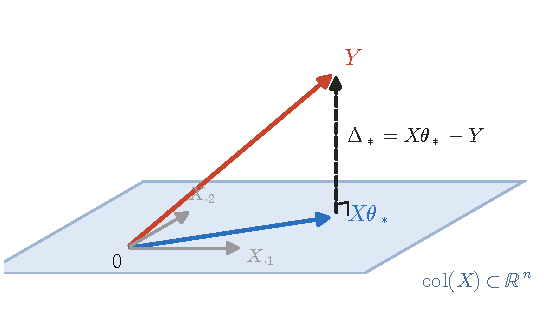
\includegraphics[width=0.5\linewidth]{fig/lsq-projection.pdf}
  \caption{Least squares, geometrically. The normal equations $X^T\Delta_*=0$ say that the residual is orthogonal to the column space of $X$, so the fitted prediction vector $X\theta_*$ is the orthogonal projection of $Y$ onto $\mathrm{col}(X)$. ``Orthogonal'' refers to the Euclidean metric $\delta_{\mu\nu}$ on the space $\R^n$ of function values on the training set.}
  \label{fig:lsq}
\end{figure}

It is worth pausing on the word ``orthogonal.'' Least squares minimizes the Euclidean ($L^2$) distance between $X\theta$ and $Y$, and the projection is orthogonal with respect to the Euclidean metric $\delta_{\mu\nu}$ on $\R^n$ --- the same metric on the space of function values that was made explicit in Section \ref{sec:geom-grads}. This metric is a \emph{choice}, hidden inside the phrase ``mean squared error.'' It declares that an error of a given size counts the same at every data point, and that errors at different data points are independent. Any other positive-definite metric $g_{\mu\nu}$ on $\R^n$ defines a different loss $\CL^g = \frac{1}{2} g_{\mu\nu}\Delta^\mu\Delta^\nu$, with a different minimizer
%
\begin{equation}
    \theta_*^g = (X^TgX)^{-1}X^TgY\,, \label{app-wls}
\end{equation}
%
which is the $g$-orthogonal projection of $Y$ onto $\mathrm{col}(X)$ (``weighted least squares''). Unless $Y$ already lies in $\mathrm{col}(X)$, different metrics give genuinely different fitted functions; see \cref{ex:app-lsq}(d). Note that $g_{\mu\nu}$ is a metric on the space of function values \emph{indexed by} the data points, not a metric on the input space $\R^d$.

\paragraph{More parameters than data, $P>n$.} If $d>n$, or more generally if the columns of $X$ are linearly dependent, then $X^TX$ is singular. The normal equations still have solutions (\cref{ex:app-lsq}(b)), but now infinitely many: an affine subspace of $\R^P$ of dimension $P-\mathrm{rank}(X)$. If moreover $X$ has full row rank $n$, then $Y\in\mathrm{col}(X)$ and \emph{every} solution interpolates the data exactly, $X\theta = Y$, with zero loss. The loss has no way to prefer one of them. Something else must make the choice; that is the subject of \cref{app:kernel}, and it is where kernels come from. Far from being an edge case, $P>n$ is the normal situation for neural networks.

\begin{exercise}[Least squares by hand]
\label{ex:app-lsq}
(a) Differentiate $\CL_\theta = \frac{1}{2}|X\theta-Y|^2$ with respect to a single coordinate $\theta^j$, assemble the components into \eqref{app-lsq-grad}, and derive the normal equations \eqref{app-normal}. Explain geometrically why they say that the residual is orthogonal to every column of $X$.
(b) Show that if $X$ has full column rank then $X^TX$ is positive definite, so that \eqref{app-lsq} is the unique minimizer. Show that the normal equations are always consistent (\emph{i.e.} $X^TY\in\mathrm{col}(X^TX)$), and that if $P>n$ they have infinitely many solutions.
(c) Fit the affine function $f(x) = \theta^1 + \theta^2 x$ to the three points $x\in\{-1,0,1\}$ with labels $y=x^2$; that is, take
%
\begin{equation*}
    X = \begin{pmatrix} 1 & -1 \\ 1 & 0 \\ 1 & 1\end{pmatrix}\,,\qquad Y = \begin{pmatrix} 1 \\ 0 \\ 1\end{pmatrix}\,.
\end{equation*}
%
Find $\theta_*$, the predictions, the residual, and the loss. Is the remaining error a failure of optimization or of representation?
(d) Repeat (c) with the weighted loss \eqref{app-wls} for $g = \mathrm{diag}(1,4,1)$, which trusts the middle data point four times as much as the others. Check that the fitted function changes.
\end{exercise}

\subsection{Linear regression with nonlinear features}
\label{app:features}

``Linear model'' is a statement about how the parameters enter, not about the shape of the fitted function. Choose, \emph{before looking at any labels}, a \emph{feature map}
%
\begin{equation}
    \psi:\R^d\to \R^P\,,\qquad \psi(x) = \big(\psi_1(x),\ldots,\psi_P(x)\big)\,,
\end{equation}
%
and consider the model
%
\begin{equation}
    f_\theta(x) = \theta\cdot\psi(x) = \sum_{i=1}^P \theta^i\,\psi_i(x)\,,\qquad \theta\in\R^P\,. \label{app-featmodel}
\end{equation}
%
This is a weighted sum of $P$ fixed shapes $\psi_i$. It can be as nonlinear in $x$ as the shapes are, but it is linear in $\theta$. Standard choices include monomials in the coordinates of $x$ up to some degree $m$ (giving $P=\binom{d+m}{m}$), Fourier modes, Gaussian bumps $e^{-|x-c_k|^2/2\sigma^2}$ centered at chosen points $c_k$, and \emph{random features} $\psi_i(x) = \phi(a_i\cdot x)$ with the $a_i$ drawn at random and then frozen --- the last being a one-hidden-layer network whose first layer is never trained.

Stacking the feature vectors of the training inputs into the $n\times P$ \emph{feature matrix}
%
\begin{equation}
    \Psi^\mu{}_i := \psi_i(x^\mu)\,, \label{app-Psi}
\end{equation}
%
the training predictions are $f = \Psi\theta$. Note that $\Psi^\mu{}_i = \pd f^\mu/\pd\theta^i$: the feature matrix is precisely the Jacobian $J$ of Section \ref{sec:features}, which for a linear model is a constant. Linear regression is the special case $\psi(x) = x$, $\Psi = X$, and \emph{everything} in \cref{app:linreg} goes through verbatim with $X$ replaced by $\Psi$: the normal equations are $\Psi^T\Psi\,\theta = \Psi^TY$; if $P\leq n$ and $\Psi$ has full column rank, the unique minimizer is $\theta_* = (\Psi^T\Psi)^{-1}\Psi^TY$; and if $P>n$ there are infinitely many interpolants.

\begin{figure}[ht]
  \centering
  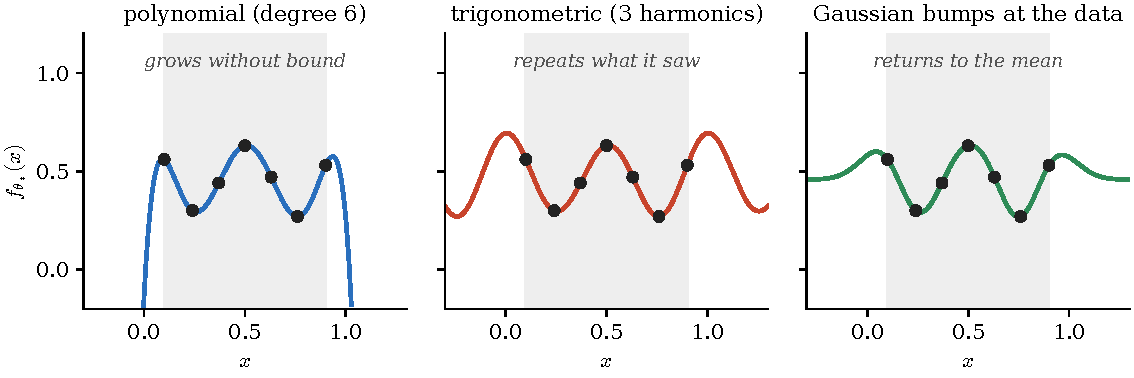
\includegraphics[width=0.98\linewidth]{fig/feature-maps.pdf}
  \caption{Choosing $\psi$ is choosing the model. The same seven data points (black), interpolated exactly by three different fixed feature maps with $P=n=7$: polynomials of degree six, trigonometric functions of period one with three harmonics, and Gaussian bumps centered at the data. All three drive the training loss to zero; they disagree everywhere outside the training range (shaded), and that disagreement was decided before the labels were read.}
  \label{fig:feature-maps}
\end{figure}

Replacing $X$ by $\Psi$ changes the algebra not at all, and changes the model completely. \Cref{fig:feature-maps} shows three feature maps, each with $P=n$, fitted to the same seven points. Each interpolates the data exactly, and they disagree everywhere else. Which is right? The data cannot say: the behavior away from the training set was fixed by the choice of $\psi$, which was made before the labels were seen. The feature map is the model's \emph{inductive bias}, made explicit.

\begin{figure}[ht]
  \centering
  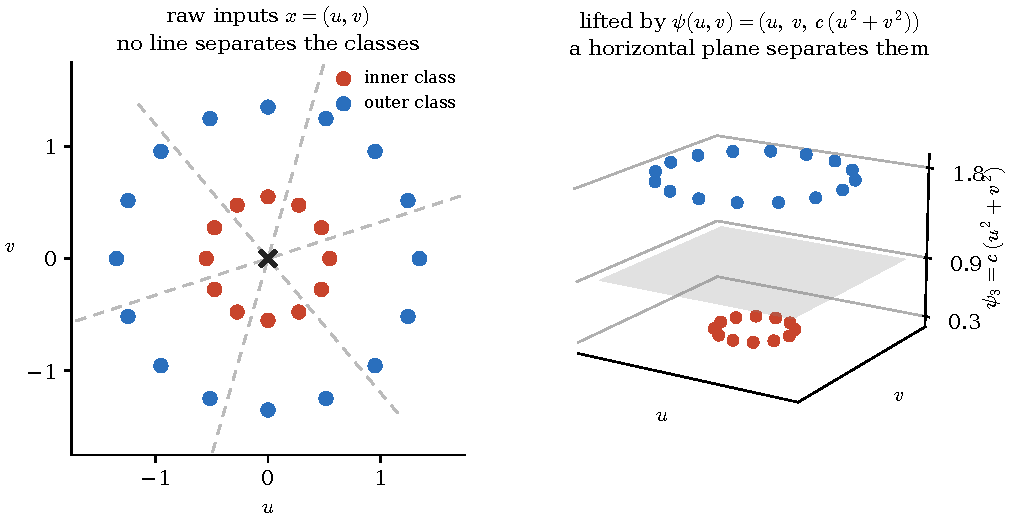
\includegraphics[width=0.98\linewidth]{fig/radial-lift.pdf}
  \caption{One fixed extra feature can make a hard problem linear. Left: two classes of points in the plane, on concentric rings. No line separates them, since the convex hull of each class contains the origin. Right: after appending the single feature $\psi_3 = c\,(u^2+v^2)$, the rings sit at two different heights, and a horizontal plane $\psi_3 = c\,r_0^2$ separates them. Nothing has been learned: we supplied the radial coordinate.}
  \label{fig:radial-lift}
\end{figure}

Why would one ever want a very large $P$? \Cref{fig:radial-lift} gives the classic answer. Two classes of points on concentric rings cannot be separated by a line in the plane. Append one fixed feature, $\psi(u,v) = (u,\,v,\,c\,(u^2+v^2))$, and the classes become separable by a plane in $\R^3$: a model that is linear in the lifted coordinates is a circle in the original ones. The price is that $P$ grows fast. All monomials of degree $3$ in $d=1000$ input coordinates already give $P = \binom{1002}{3} \approx 1.7\times 10^8$, and Gaussian bumps centered at every point of a continuum give $P=\infty$. Yet there are only $n$ data points, and the fit is determined by $n$ numbers. Nothing about the problem should require a $P\times P$ inverse --- so where does $P$ actually enter? Answering that question honestly is the content of the next two sections.

\begin{exercise}[A three-point feature calculation]
\label{ex:app-features}
Take the same three points $x\in\{-1,0,1\}$ with labels $y=x^2$ as in \cref{ex:app-lsq}(c), but now the feature map $\psi(x) = (1,\,\sqrt2\,x,\,x^2)$.
(a) Form the feature matrix $\Psi$ and find coefficients $\theta$ that interpolate all three labels. The representational failure of \cref{ex:app-lsq}(c) is gone: what changed?
(b) Explain precisely how the predictor can be nonlinear in $x$ while the regression problem remains linear.
(c) If the last feature is replaced by $c\,x^2$ for some $c\neq 0$, what changes: the fitted function, its coefficient, or both?
(d) Write the inner product $K(x,z) := \psi(x)\cdot\psi(z)$ in closed form, without vector notation. This is a preview of \cref{app:kernel}.
\end{exercise}

\subsection{Kernel regression}
\label{app:kernel}

Return to the overparametrized case $P>n$, and assume that $\Psi$ has full row rank $n$ (the generic situation), so that there is a $(P-n)$-dimensional affine family of exact interpolants $\Psi\theta = Y$. To choose one, we need a criterion that the loss does not provide. The standard choice is the interpolant of \emph{minimum norm},
%
\begin{equation}
    \theta_* := \underset{\Psi\theta = Y}{\mathrm{arg\,min}}\; |\theta|^2\,. \label{app-minnorm}
\end{equation}
%
This introduces a \emph{second} implicit Euclidean metric --- now $\delta_{ij}$ on parameter space $\R^P$, the metric that also defines gradient descent in Section \ref{sec:geom-grads}. (\Cref{app:linreg} used $\delta_{\mu\nu}$ on the space $\R^n$ of function values.) The two metrics play dual roles: the first decides how to fit when the data cannot be matched, the second decides which fit to choose when it can.

To solve \eqref{app-minnorm}, introduce Lagrange multipliers $\alpha\in\R^n$ for the $n$ constraints and extremize $\frac{1}{2}|\theta|^2 - \alpha\cdot(\Psi\theta - Y)$. Stationarity in $\theta$ gives
%
\begin{equation}
    \theta_* = \Psi^T\alpha = \sum_{\mu=1}^n \alpha_\mu\,\psi(x^\mu)\,. \label{app-representer}
\end{equation}
%
This is the key structural fact: however large $P$ is, the minimum-norm solution lies in the $n$-dimensional subspace of $\R^P$ spanned by the feature vectors of the training inputs, and is described by $n$ numbers. (In the language of Section \ref{sec:features}, $\theta_*$ lies in the row space of the Jacobian.) The constraint $\Psi\theta_* = Y$ then becomes $\Psi\Psi^T\alpha = Y$, an $n\times n$ linear system. Define the \emph{kernel} and its \emph{Gram matrix} on the training set,
%
\begin{equation}
    K(x,x') := \psi(x)\cdot\psi(x') = \sum_{i=1}^P \psi_i(x)\psi_i(x')\,,\qquad
    \hat K^{\mu\nu} := K(x^\mu,x^\nu) = (\Psi\Psi^T)^{\mu\nu}\,. \label{app-kernel}
\end{equation}
%
The kernel is an inner product of feature vectors: a notion of \emph{similarity} between inputs, fixed once $\psi$ is fixed, and involving no labels. The Gram matrix is symmetric and positive semidefinite, since $c^T\hat K c = |\Psi^Tc|^2\geq 0$; it is positive definite exactly when $\Psi$ has full row rank, which we assumed. Then $\alpha = \hat K^{-1}Y$, and the prediction at an arbitrary input $x$ is
%
\begin{equation}
    f_*(x) = \theta_*\cdot\psi(x) = \sum_{\mu=1}^n \alpha_\mu K(x,x^\mu) = \sum_{\mu,\nu=1}^n K(x,x^\mu)\,\hat K^{-1}_{\mu\nu}\,y^\nu\,. \label{app-kernel-reg}
\end{equation}
%
This is \emph{kernel regression} (more precisely, kernel interpolation). The feature map has disappeared from both the fit and the prediction. To fit, one needs $K$ on pairs of training points; to predict, one needs $K$ between the test point and the training points; no feature vector is ever constructed. The prediction is a weighted sum of similarities to the training points, with weights $\alpha$ that depend on the labels --- but the labels only reweight the training points, they never change which inputs $K$ considers similar.

Compare \eqref{app-kernel-reg} with the late-time mean \eqref{NTK-GP} of a lazily trained network: they are the same formula, with $\hat K$ in place of the NTK. This is no coincidence. For any model linear in its parameters the Jacobian is $J=\Psi$, so the NTK \eqref{NTK} is
%
\begin{equation}
    \Theta^{\mu\nu} = (JJ^T)^{\mu\nu} = \hat K^{\mu\nu}\,, \label{app-NTK-is-K}
\end{equation}
%
constant in time. Moreover, gradient flow finds the minimum-norm solution: $\dot\theta = -\eta\,\Psi^T\Delta$ always points along the row space of $\Psi$, so $\theta(t)-\theta_0$ stays in that $n$-dimensional subspace and converges to the interpolant nearest to $\theta_0$ --- for $\theta_0 = 0$, to $\theta_*$ (\cref{ex:app-kernel}(c)). This is the simplest instance of the \emph{implicit bias} of gradient descent, and it is the Euclidean metric on parameter space entering through the back door: the flow is defined by $\delta^{ij}$, and so is the norm that it ends up minimizing.

\paragraph{The kernel trick.} There are two readings of \eqref{app-kernel-reg}. Read from the feature side, it rewrites a $P\times P$ problem as an $n\times n$ one. Read from the kernel side, it says the feature map is dispensable: any function $K(x,x')$ that arises as an inner product of features will do, whether or not one can write the features down. For $x,z\in\R^2$ and $\psi(x) = (x_1^2,\,\sqrt2\,x_1x_2,\,x_2^2)$, one checks that $\psi(x)\cdot\psi(z) = (x\cdot z)^2$: a single dot product, squared, stands in for three features. In $d$ dimensions, $K(x,z) = (x\cdot z)^m$ costs $O(d)$ to evaluate and stands in for all $\binom{d+m-1}{m}$ monomials of degree $m$. The Gaussian kernel $K(x,z) = e^{-|x-z|^2/2\sigma^2}$ corresponds to an infinite-dimensional feature map that no one ever writes down. Conversely, any symmetric $K$ all of whose Gram matrices are positive semidefinite arises from some feature map (Mercer's theorem): the eigenfunctions of $K$, weighted by the square roots of its eigenvalues, furnish one (\emph{cf.} Sections \ref{sec:GP} and \ref{sec:Bayes-kernel}). This is a trade, not a free lunch. The feature route scales with $P$ and the kernel route with $n$; with many examples and few features, the explicit route is the cheap one.

\begin{exercise}[Minimum-norm interpolation and the kernel]
\label{ex:app-kernel}
(a) Carry out the Lagrange-multiplier computation leading to \eqref{app-representer}--\eqref{app-kernel-reg}. Alternatively, use the singular value decomposition $\Psi = USV^T$ of Section \ref{sec:features} to show that the minimum-norm interpolant is $\theta_* = \Psi^T(\Psi\Psi^T)^{-1}Y$, and write it in terms of $U,S,V$.
(b) Show that $c^T\hat Kc = |\Psi^Tc|^2\geq 0$ for all $c\in\R^n$. Interpret a zero eigenvalue of $\hat K$ as a linear combination of training examples that vanishes in feature space. What does it take for $\hat K$ to be invertible?
(c) Show that under gradient flow $\dot\theta = -\eta\,\Psi^T(\Psi\theta - Y)$ the displacement $\theta(t)-\theta_0$ stays in the row space of $\Psi$ for all $t$; derive $\Delta(t) = e^{-\eta t\hat K}\Delta(0)$; and conclude that, for invertible $\hat K$, the flow converges to the interpolant closest to $\theta_0$. Derive \eqref{NTK-learn} for this model, with $\Theta = \hat K$.
(d) Verify that $\psi(x)\cdot\psi(z) = (x\cdot z)^2$ for $\psi(x) = (x_1^2,\sqrt2\,x_1x_2,x_2^2)$, and explain why the $\sqrt2$ is not decoration. Which feature map on $\R$ produces the kernel $(1+xz)^2$ of \cref{ex:app-features}(d)? How many features does $(x\cdot z)^m$ on $\R^d$ stand in for?
\end{exercise}

\subsection{Kernel ridge regression}
\label{app:ridge}

Rather than imposing the minimum-norm criterion as a hard constraint, one can add it to the loss as a penalty. For $\lambda>0$, \emph{ridge regression} minimizes
%
\begin{equation}
    \CL_\lambda(\theta) := \frac{1}{2}|\Psi\theta - Y|^2 + \frac{\lambda}{2}|\theta|^2\,. \label{app-ridge-loss}
\end{equation}
%
The two terms measure distance to the data with $\delta_{\mu\nu}$ and distance to the origin with $\delta_{ij}$: ridge regression is a weighted compromise between the two metrics of \cref{app:linreg,app:kernel}, with $\lambda$ setting the exchange rate. (In the training of neural networks the penalty is called \emph{weight decay}.) The penalty does two jobs at once. When $P>n$ it selects one solution out of infinitely many; and for any $P$ it makes the problem well posed even when the features are redundant or the labels are noisy. Note that the penalty is not invariant under rescaling features: it decides what counts as a ``large'' coefficient in the coordinates $\psi$ that were supplied.

The gradient is $\Psi^T(\Psi\theta - Y) + \lambda\theta$, so the stationarity condition is
%
\begin{equation}
    (\Psi^T\Psi + \lambda I_P)\,\theta = \Psi^TY\,. \label{app-ridge-normal}
\end{equation}
%
The matrix on the left is positive definite for every $\lambda>0$, whatever the rank of $\Psi$, since $v^T(\Psi^T\Psi+\lambda I_P)v = |\Psi v|^2+\lambda|v|^2>0$. So there is always a unique minimizer,
%
\begin{equation}
    \theta_\lambda = (\Psi^T\Psi + \lambda I_P)^{-1}\Psi^TY\,, \label{app-ridge-P}
\end{equation}
%
at the price of a $P\times P$ inverse. To move the inverse to the $n\times n$ side, expand and regroup the product
%
\begin{equation}
    \Psi^T(\Psi\Psi^T + \lambda I_n) = \Psi^T\Psi\Psi^T + \lambda\Psi^T = (\Psi^T\Psi + \lambda I_P)\Psi^T\,.
\end{equation}
%
Both bracketed matrices are positive definite, so multiplying by their inverses on the appropriate sides gives the \emph{push-through identity}
%
\begin{equation}
    (\Psi^T\Psi + \lambda I_P)^{-1}\Psi^T = \Psi^T(\Psi\Psi^T + \lambda I_n)^{-1}\,. \label{app-pushthrough}
\end{equation}
%
Nothing was cancelled --- $\Psi^T$ is rectangular and has no inverse --- and that is precisely why the identity holds. Substituting into \eqref{app-ridge-P}, the ridge solution again lies in the span of the training feature vectors, $\theta_\lambda = \Psi^T\alpha_\lambda$, now with $\alpha_\lambda = (\hat K+\lambda I_n)^{-1}Y$, and the prediction at a new input is
%
\begin{equation}
    f_\lambda(x) = \sum_{\mu,\nu=1}^n K(x,x^\mu)\,\big(\hat K + \lambda I_n\big)^{-1}_{\mu\nu}\,y^\nu\,. \label{app-krr}
\end{equation}
%
This is \emph{kernel ridge regression}, the central formula of this appendix. As $\lambda\to 0$ it reduces to the minimum-norm interpolant \eqref{app-kernel-reg} when $\hat K$ is invertible, and in general to the least-squares solution of minimum norm (\cref{ex:app-ridge}(c)). As $\lambda\to\infty$, $\theta_\lambda\to 0$.

Formula \eqref{app-krr} is exactly the posterior mean of \cref{ex:kernel-ridge}, with ridge parameter $\lambda = \beta^{-1}$ --- there derived for the infinite-width Gaussian process, here for a finite linear model. The Bayesian reading is worth making explicit. With a Gaussian likelihood $\propto e^{-\frac{\beta}{2}|\Psi\theta-Y|^2}$ and a Gaussian prior $\theta\sim\CN(0,\sigma^2 I_P)$, the loss \eqref{app-ridge-loss} is $-\beta^{-1}\log$ of the posterior density, up to a constant, with $\lambda = 1/(\beta\sigma^2)$. Ridge regression is thus maximum a posteriori estimation. The prior pushed forward to $f_\theta(x) = \theta\cdot\psi(x)$ is a Gaussian process with kernel $\sigma^2K(x,x')$, a finite-$P$ instance of Section \ref{sec:GP}, and the posterior mean of \cref{ex:kernel-ridge} for this process reproduces \eqref{app-krr}.

\paragraph{Spectral view.} With the singular value decomposition $\Psi = USV^T$ of Section \ref{sec:features}, the Gram matrix is $\hat K = US^2U^T$, with eigenvalues $s_a^2$ and orthonormal eigenvectors $u_a\in\R^n$: the ``features'' of Section \ref{sec:features}, \emph{i.e.} the natural modes in the space of function values. The ridge predictions on the training set are $f_\lambda = \Psi\theta_\lambda = \hat K(\hat K+\lambda I_n)^{-1}Y$, or, mode by mode,
%
\begin{equation}
    f_\lambda = \sum_a \frac{s_a^2}{s_a^2+\lambda}\,(u_a\cdot Y)\,u_a\,. \label{app-ridge-filter}
\end{equation}
%
Ridge regression is a \emph{spectral filter}: modes of the data with $s_a^2\gg\lambda$ are fit, modes with $s_a^2\ll\lambda$ are suppressed, and the crossover is at $s_a^2\approx\lambda$. Compare gradient flow from $\theta_0 = 0$ on the unpenalized loss, whose training predictions are, by \eqref{D-converge},
%
\begin{equation}
    f(t) = \sum_a \big(1-e^{-\eta t s_a^2}\big)\,(u_a\cdot Y)\,u_a\,. \label{app-flow-filter}
\end{equation}
%
This is also a spectral filter, with $1/\eta t$ playing the role of $\lambda$: \emph{early stopping} regularizes much as ridge does. But the two filters have different shapes (\cref{fig:filters}), and no choice of $\lambda$ reproduces a given stopping time on every mode at once (\cref{ex:app-filters}). This is the precise content of the remark closing Section \ref{sec:Bayes-kernel}, that the inverse temperature of Bayesian learning and the training time of gradient descent play analogous roles.

\begin{figure}[ht]
  \centering
  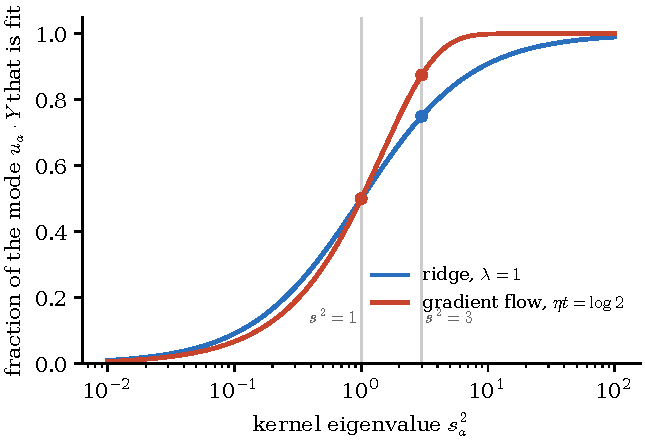
\includegraphics[width=0.55\linewidth]{fig/ridge-filters.pdf}
  \caption{Ridge regression and early-stopped gradient flow as spectral filters: the fraction of a data mode $u_a\cdot Y$ that is fit, as a function of the mode's kernel eigenvalue $s_a^2$. The two are tuned to agree on the mode with $s^2=1$, and disagree elsewhere; the dots mark the two-mode example of \cref{ex:app-filters}.}
  \label{fig:filters}
\end{figure}

\begin{exercise}[Ridge regression, two ways]
\label{ex:app-ridge}
(a) Derive \eqref{app-ridge-normal} and \eqref{app-ridge-P}, and prove that $\Psi^T\Psi+\lambda I_P$ is invertible even when $\Psi$ is rank deficient.
(b) Prove the push-through identity \eqref{app-pushthrough} and deduce \eqref{app-krr}. Explain why ``cancelling $\Psi^T$'' is not a valid step, and why the identity is nevertheless true. (It is a special case of $A(BA+I)^{-1} = (AB+I)^{-1}A$.)
(c) What happens as $\lambda\to\infty$? Using the SVD, show that $\theta_\lambda$ applies the scalar filter $s/(s^2+\lambda)$ to each singular value $s$ of $\Psi$, and hence that as $\lambda\to 0$ it converges to the least-squares solution of minimum norm. When does this limit interpolate the labels exactly?
(d) Return to $x\in\{-1,0,1\}$, $y=x^2$ and the kernel $K(x,z) = (1+xz)^2$ of \cref{ex:app-features}. With $\lambda = 1$, verify that
%
\begin{equation*}
    \hat K = \begin{pmatrix} 4 & 1 & 0 \\ 1 & 1 & 1 \\ 0 & 1 & 4 \end{pmatrix}\,,\qquad
    \alpha_\lambda = \frac{1}{4}\begin{pmatrix} 1 \\ -1 \\ 1 \end{pmatrix}\,,
\end{equation*}
%
and predict at $z=2$ using only kernel evaluations. Compare with the interpolant of \cref{ex:app-features}(a), which predicts $z^2=4$ there, and explain the direction of the discrepancy.
(e) The feature route solves a $P\times P$ system and the kernel route an $n\times n$ one. When is each attractive?
\end{exercise}

\begin{exercise}[Early stopping vs.\ ridge, on two data points]
\label{ex:app-filters}
Take $n=2$ training points with Gram matrix and labels
%
\begin{equation*}
    \hat K = \begin{pmatrix} 2 & 1 \\ 1 & 2\end{pmatrix}\,,\qquad Y = \begin{pmatrix} 2 \\ 0 \end{pmatrix}\,,
\end{equation*}
%
and initial predictions $f(0) = 0$.
(a) Verify the eigenpairs $u_\pm = \frac{1}{\sqrt2}(1,\pm 1)^T$ with $s_\pm^2 = 3, 1$, and decompose $Y$ into these modes.
(b) Using \eqref{app-flow-filter}, find the training predictions $f(t)$ under gradient flow, and evaluate them at $\eta t = \log 2$. Why do both the eigenvalue $s_a^2$ and the initial projection $u_a\cdot Y$ matter for what is visible during training?
(c) Using \eqref{app-ridge-filter}, find the ridge predictions for $\lambda = 1$. The two filters agree on the mode with $s^2 = 1$; show that the ridge parameter matching gradient flow at time $t$ on a mode with eigenvalue $s^2$ is $\lambda_{\rm eff}(s^2,t) = s^2/(e^{\eta t s^2}-1)$, which depends on the mode --- so early stopping is not ridge regression.
(d) State precisely what ``spectral bias'' means for this finite, fixed-kernel calculation. What additional structure would be needed to turn it into a claim about Fourier frequencies, about robustness to label noise, or about test error?
\end{exercise}

\subsection{Linearized networks are kernel ridge regressors}
\label{app:linearized}

Now let $f_\theta$ be a neural network, with $\theta\in\R^P$ the vector of \emph{all} its weights and biases. It is not linear in $\theta$. But its linearization around the initialization $\theta_0$, the ansatz \eqref{f-lin},
%
\begin{equation}
    f^{\rm lin}_\theta(x) = f_{\theta_0}(x) + (\theta-\theta_0)\cdot\nabla_\theta f_{\theta_0}(x)\,, \label{app-flin}
\end{equation}
%
is a model of the form \eqref{app-featmodel}. Compare term by term. The parameters are the displacement $\delta\theta := \theta-\theta_0\in\R^P$. The feature map is
%
\begin{equation}
    \psi(x) = \nabla_\theta f_{\theta_0}(x)\in\R^P\,, \label{app-tangent-features}
\end{equation}
%
the \emph{tangent features}: one number per parameter, the sensitivity of the output at $x$ to that parameter, evaluated at initialization and then frozen. And the constant offset $f_{\theta_0}(x)$ is absorbed by shifting the labels to
%
\begin{equation}
    \tilde y^\mu := y^\mu - f_{\theta_0}(x^\mu) = -\Delta^\mu(0)\,. \label{app-shifted-labels}
\end{equation}
%
The offset matters: the linearized model is fit to the \emph{residuals at initialization}, not to the raw labels. The feature matrix \eqref{app-Psi} is the Jacobian at initialization, $\Psi = J_0$, and the Gram matrix \eqref{app-kernel} is
%
\begin{equation}
    \hat K = J_0J_0^T = \Theta_0\,,\qquad K(x,x') = \Theta(x,x') = \nabla_\theta f_{\theta_0}(x)\cdot\nabla_\theta f_{\theta_0}(x')\,, \label{app-K-is-NTK}
\end{equation}
%
the neural tangent kernel \eqref{NTK} at initialization, extended to arbitrary pairs of inputs as in \cref{ex:ntk-test}. Everything in \cref{app:kernel,app:ridge} now applies verbatim. In particular, ridge regression on the linearized network with penalty $\frac{\lambda}{2}|\theta-\theta_0|^2$ --- weight decay toward the initialization --- gives, by \eqref{app-krr},
%
\begin{equation}
    f^{\rm lin}_\lambda(x) = f_{\theta_0}(x) - \sum_{\mu,\nu=1}^n \Theta(x,x^\mu)\,\big(\Theta_0 + \lambda I_n\big)^{-1}_{\mu\nu}\,\Delta^\nu(0)\,. \label{app-lin-krr}
\end{equation}
%
At $\lambda\to 0$ this is the $t\to\infty$ limit of \eqref{NTK-learn}, the minimum-norm interpolant of the residuals; and the finite-time solution \eqref{NTK-learn} is its early-stopped cousin, in the sense of \eqref{app-flow-filter}. The kernel trick is not a convenience here but a necessity: $P$ is the parameter count of the network, often $10^7$ or more, while $\Theta_0$ is $n\times n$.

Two remarks on what is and is not being claimed. First, for the linearized model $f^{\rm lin}$ everything above is exact, and its kernel is constant by construction. For the actual network, \eqref{app-flin} is an ansatz. Section \ref{sec:NTK-const} shows that it becomes exact in the large-width limit at fixed depth and data; whether and when it is a good approximation otherwise --- and what happens when the tangent features move --- is the subject of Sections \ref{sec:MFT}--\ref{sec:DMFT}, not of this appendix. Second, the initialization $\theta_0$ is random, so $f_{\theta_0}$, the tangent features, and the kernel $\Theta_0$ are all random too, and \eqref{app-lin-krr} is the trained function for one draw. Averaging over draws, at large width where $\Theta_0$ becomes deterministic, gives the Gaussian process \eqref{NTK-GP}.

\begin{exercise}[Tangent features of a one-hidden-layer network]
\label{ex:app-tangent}
Consider $f_\theta(x) = \sum_{i=1}^N c_i\,\phi(a_i\cdot x)$ with $\theta = (c_i, a_i)_{i=1}^N$, so that $P = N(d+1)$.
(a) Compute the tangent features $\nabla_\theta f_{\theta_0}(x)$, and show that the tangent kernel is
%
\begin{equation*}
    \Theta(x,x') = \sum_{i=1}^N \phi(a_i\cdot x)\,\phi(a_i\cdot x') + \sum_{i=1}^N c_i^2\,\phi'(a_i\cdot x)\,\phi'(a_i\cdot x')\,(x\cdot x')\,.
\end{equation*}
%
(b) Suppose only the output weights $c$ are trained, with the $a_i$ frozen at their random initial values. Show that this is exactly a fixed-feature model \eqref{app-featmodel} with random features, that its linearization is exact, and that its kernel is the first term above. Which term do you get by training only the $a_i$?
(c) Show that gradient flow with weight decay toward the initialization, $\dot\theta = -\eta\big[\nabla_\theta \CL + \lambda(\theta-\theta_0)\big]$, applied to the linearized model $f^{\rm lin}$, converges to the ridge solution \eqref{app-lin-krr} for every $\lambda>0$ and from any starting point.
(d) Check that \eqref{app-lin-krr} at $\lambda\to 0$ coincides with \eqref{NTK-learn} at $t\to\infty$.
\end{exercise}


%===============================================================================
%===============================================================================
\section{Solutions to exercises}
\label{app:solutions}

Worked solutions to the exercises, in the order in which the exercises appear. (Instructors: uncommenting \verb|\solutionsfalse| in the preamble removes this appendix's contents, and all other solution boxes, from the compiled PDF.)

\begin{solution}[ex:cumulants]
\begin{enumerate}
    \item Differentiating under the integral, $\pd_J\log Z = \frac{1}{Z}\int d\theta\,\CO\,e^{-\beta E+J\CO} = \E_J(\CO)$, which at $J=0$ is $\E(\CO)$; since $F=-\log Z$, this is $-\pd_JF|_0$. Once more, $\pd_J^2\log Z = \E_J(\CO^2)-\E_J(\CO)^2 = \mathrm{Var}_J(\CO)$.
    \item Using $\pd_J\E_J(\CO^k) = \E_J(\CO^{k+1}) - \E_J(\CO^k)\E_J(\CO)$ on $\pd_J^2\log Z = \E_J(\CO^2)-\E_J(\CO)^2$ gives
    $\kappa_3 = \E(\CO^3) - 3\E(\CO^2)\E(\CO) + 2\E(\CO)^3$. Expanding $\E[(\CO-\E\CO)^3] = \E(\CO^3) - 3\E(\CO^2)\E(\CO) + 3\E(\CO)\E(\CO)^2 - \E(\CO)^3$ gives the same expression.
    \item For $\CO\sim\CN(\mu,\sigma^2)$ (or more generally when $\CO$ is Gaussian under $p_\beta$), $\E(e^{J\CO}) = e^{J\mu+J^2\sigma^2/2}$, so $\log Z(J) = \log Z(0) + J\mu + \frac{1}{2}J^2\sigma^2$ is quadratic and every derivative beyond the second vanishes. One more derivative of the pattern in (b), with $\bar\CO := \CO - \E\CO$, gives $\kappa_4 = \E(\bar\CO^4) - 3\,\E(\bar\CO^2)^2$; for a Gaussian $\E(\bar\CO^4) = 3\sigma^4$, so $\kappa_4 = 0$ while the fourth centered moment is not.
    \item $\pd_\beta\log Z = -\frac{1}{Z}\int E\,e^{-\beta E} = -\E(E)$, so $\pd_\beta F = \E(E)$; $\pd_\beta^2\log Z = \E(E^2)-\E(E)^2$, so $-\pd_\beta^2F = \mathrm{Var}(E)$; and $\pd_\beta^3\log Z = -\kappa_3(E)$ by the same computation as (b) with $J\to-\beta$, so $\kappa_3(E) = \pd_\beta^3F$.
\end{enumerate}
\end{solution}

\begin{solution}[ex:anatomy]
\begin{enumerate}
    \item $p_i$ is the fraction of $Z$ contributed by basin $i$. With $\varphi_1-\varphi_2\approx\Delta\varphi'\,\Delta B$ near the crossing, $p_2 = (1+e^{-N(\varphi_1-\varphi_2)})^{-1}\approx(1+e^{-N\Delta\varphi'\Delta B})^{-1}$. The switch happens over the window $|\Delta B|\lesssim 1/(N\Delta\varphi')$, which shrinks with system size.
    \item Differentiating $\varphi = -\frac{1}{N}\log(e^{-N\varphi_1}+e^{-N\varphi_2})$ gives $\pd_B\varphi = p_1\varphi_1' + p_2\varphi_2'$ exactly; near $B_c$ the slopes are $\approx\varphi_i'(B_c)$. Directly from the integral, $\pd_B\varphi = -\frac{1}{N}\pd_B\log Z = \frac{1}{Z}\int d\theta\,\pd_BE\,e^{-NE} = \E[\pd_BE]$: the control parameter is itself a source, coupling to $\CO = \pd_BE$. \emph{Sketch:} at finite $N$, $\pd_B\varphi$ is a sigmoid interpolating from $\varphi_1'(B_c)$ to $\varphi_2'(B_c)$ over the window of (a); as $N\to\infty$, $\varphi\to\min(\varphi_1,\varphi_2)$, continuous with a kink at $B_c$, and $\pd_B\varphi$ becomes a step of height $\Delta\varphi'$.
    \item $\pd_Bp_1 = \pd_B\frac{e^{-N\varphi_1}}{e^{-N\varphi_1}+e^{-N\varphi_2}} = -Np_1p_2(\varphi_1'-\varphi_2')$ and $\pd_Bp_2 = -\pd_Bp_1$. Then $\pd_B^2\varphi = (\pd_Bp_1)\varphi_1' + (\pd_Bp_2)\varphi_2' + p_1\varphi_1''+p_2\varphi_2'' = -Np_1p_2(\Delta\varphi')^2 + p_1\varphi_1''+p_2\varphi_2''$. \emph{Sketch:} a smooth background from the $\varphi_i''$ terms plus a peak at $B_c$ of height $\approx N(\Delta\varphi')^2/4$ and width $\sim1/(N\Delta\varphi')$, the nascent delta function of the $N=\infty$ kink. For the variance identity: with $\CO=\pd_BE$ independent of $B$, differentiating $\pd_B\varphi = \E(\CO)$ once more gives $\pd_B^2\varphi = -N[\E(\CO^2)-\E(\CO)^2]$, so $-\pd_B^2\varphi = N\,\mathrm{Var}(\CO)\geq0$, which is why the curve is a peak and not a dip. The two-branch formula exhibits the leading piece of this variance: $\CO\approx\varphi_1'$ in one basin and $\approx\varphi_2'$ in the other, and the variance of that two-point mixture is exactly $p_1p_2(\Delta\varphi')^2$.
    \item See \cref{fig:first-order}. The peak in the right panel grows in proportion to $N$; a crossover's bump would saturate.
\end{enumerate}
\begin{figure}[H]
  \centering
  \includegraphics[width=0.98\linewidth]{fig/first-order-smoothing.pdf}
  \caption{Anatomy of a first-order transition at finite $N$, in the minimal two-branch model $\varphi_1(B) = 0.3\,(B-B_c)$, $\varphi_2\equiv0$, with the control parameter written as $\alpha$. Left: the branch free energies cross at $B_c$; the limiting free-energy density is their minimum, which has a kink. Middle: at finite $N$, $\pd_B\varphi$ is the probability-weighted average of the branch slopes \eqref{dF-sigmoid}, a sigmoid of width $\propto1/N$. Right: the susceptibility \eqref{chi-peak} peaks at $B_c$ with height $\propto N$ and width $\propto1/N$.}
  \label{fig:first-order}
\end{figure}
\end{solution}

\begin{solution}[ex:ising]
\begin{enumerate}
    \item $R = \frac{1}{N}\sum_i\theta_i\theta_i^* = \frac{1}{N}\sum_is_i$ since $(\theta_i^*)^2 = 1$. The map $\theta\mapsto s$ is a bijection of the hypercube (a ``gauge transformation''), so the uniform measure goes to the uniform measure, and the perceptron's order parameter is literally a magnetization.
    \item Both labels depend only on the projection of $x$ onto $\mathrm{span}(\theta,\theta^*)$, which is an isotropic two-dimensional Gaussian. The decision boundaries are two diameters at angle $\vartheta = \arccos R$; the signs disagree exactly on the double wedge between them, of angular fraction $2\vartheta/2\pi = \vartheta/\pi$. Note that the answer does not depend on $N$, and holds for any $\theta$ with $|\theta|^2 = N$, binary or not.
    \item A student at overlap $R$ agrees with the teacher on exactly $\frac{1+R}{2}N$ coordinates ($s_i = +1$), giving the binomial count; Stirling gives $h(R)$, the binary entropy at magnetization $R$. Note $h(0) = \log2$ and $h(1) = 0$: the latter is \emph{finite}, because exactly one state sits at $R=1$.
    \item Independence over examples gives the $n$-th power. Trading the sum for an integral, $\frac{1}{2^N}\sum_\theta\to\int dR\,e^{N[h(R)-\log2]}$, and $(1-\varepsilon)^n = e^{N\alpha\log(1-\varepsilon)}$; collecting exponents gives $s(R)$ as stated. (The $\log2$ normalizes $s(0) = 0$ at $\alpha=0$.)
    \item The curves are shown in \cref{fig:ising-perceptron-action}. At $\alpha=0$, $s = \log2-h(R)$ has a single minimum at $R=0$, the bulk of the hypercube. As $\alpha$ grows, the interior minimum drifts toward larger $R$ and its value rises (note $s(0) = \alpha\log2$), while $R=1$ stays pinned at $s(1) = \log2$. For $\alpha$ large enough there are two competing local minima separated by a barrier: exactly the two-basin structure of \cref{ex:anatomy}. One should therefore expect a first-order transition at the load where the interior minimum's value crosses $\log2$, near $\alpha\approx1.45$ from the plot; at $\alpha=1.7$ the interior minimum survives only as a metastable dip above $\log2$. No transition is expected at small $\alpha$, where the interior minimum is the only relevant one and moves smoothly.
    \begin{figure}[H]
      \centering
      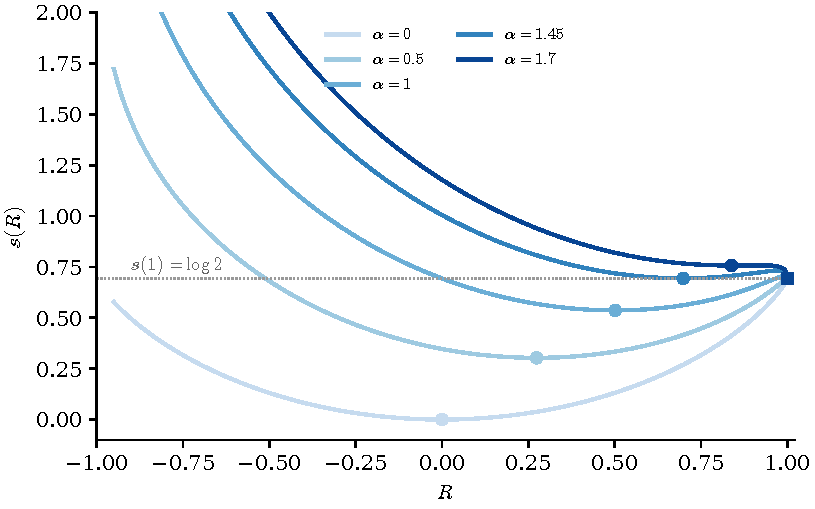
\includegraphics[width=0.66\linewidth]{fig/ising-perceptron-action.pdf}
      \caption{The annealed action $s(R)$ of the Ising perceptron, \eqref{perc-action}, for several loads. Interior local minima are marked with circles; the teacher state $R=1$, where $s(1) = \log2$ exactly, with squares. The two basins exchange dominance near $\alpha\approx1.45$.}
      \label{fig:ising-perceptron-action}
    \end{figure}
    \item At $R=1$: $h(1) = 0$ and $\varepsilon(1) = 0$, so $s(1) = \log2$ for all $\alpha$. Near $R=1$ with $\delta = 1-R$: $h(1-\delta) = \frac{\delta}{2}\log\frac{2}{\delta}+O(\delta)$, while $\arccos(1-\delta)\approx\sqrt{2\delta}$ gives data cost $-\alpha\log(1-\varepsilon)\approx\alpha\sqrt{2\delta}/\pi$. Since $\sqrt\delta\gg\delta\log(1/\delta)$ as $\delta\to0$, $s(1-\delta)>s(1)$: a basin around the teacher at every $\alpha>0$. It is protected by the singular cost of the first errors, which is what a smooth well cannot provide.
    \item Minimizing $s$ over the interior numerically (\cref{fig:ising-perceptron-phase}, left), the interior branch value crosses $s(1) = \log2$ at $\alpha_c\approx1.45$, with minimizer $R^*\approx0.70$ and $\varepsilon^* = \arccos(0.70)/\pi\approx0.25$. The order parameter jumps from $0.70$ to $1$ (middle panel). With $\alpha$ as the control parameter of \cref{ex:anatomy}: $\varphi(\alpha) = \min_Rs(R)$ has a kink at $\alpha_c$; at finite $N$, $\pd_\alpha\varphi = \E[-\log(1-\varepsilon(R))]$ is a sigmoid interpolating between the branch slopes $-\log(1-\varepsilon(R^*))\approx0.29$ and $0$, over a window of width $\sim1/(N\Delta\varphi')$ (right panel), and $-\pd_\alpha^2\varphi$ is a peak of height $\propto N$. The role of the latent heat is played by the jump in $-\log(1-\varepsilon)$, the per-example log-likelihood released when the student snaps onto the teacher. Past $\alpha_c$ the interior minimum survives as a local minimum until the \emph{spinodal} $\alpha\approx1.73$, where it merges with the barrier and disappears. In the window $1.45\lesssim\alpha\lesssim1.73$ a local learning dynamics (flipping a few weights at a time to improve alignment) can stay stuck at $\varepsilon\approx0.25$ even though perfect generalization is thermodynamically dominant: the information needed to identify the teacher is present in the data before the dynamics can find it, and generalization arrives abruptly and later than the data first permits. This is the metastability of Section \ref{sec:phase-transitions}, and a prototype of the delayed transitions of Section \ref{sec:grok}. (The exact, quenched treatment \cite{gyorgyi1990first,engel2001statistical} moves the transition to $\alpha_c\approx1.245$ but changes nothing structurally.)
    \begin{figure}[H]
      \centering
      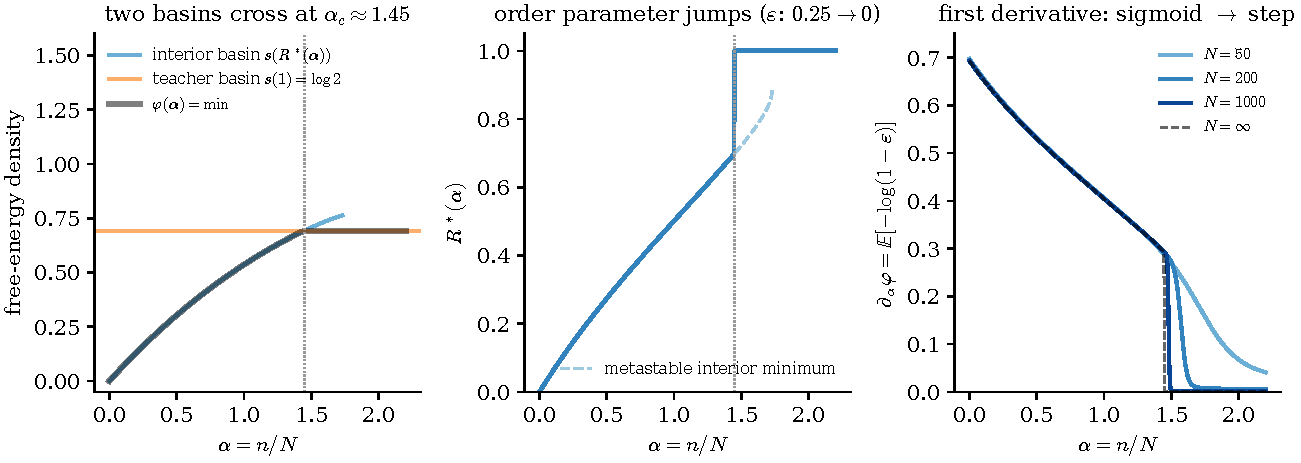
\includegraphics[width=0.98\linewidth]{fig/ising-perceptron-phase.pdf}
      \caption{The Ising perceptron's phase transition. Left: the free-energy densities of the interior basin, $s(R^*(\alpha))$, and of the teacher basin, $s(1) = \log2$, cross at $\alpha_c\approx1.45$; the limiting $\varphi(\alpha)$ is their minimum, with a kink. Middle: the order parameter $R^*(\alpha)$ jumps from $0.70$ to $1$; the dashed continuation is the metastable interior minimum, which disappears at the spinodal $\alpha\approx1.73$. Right: at finite $N$, $\pd_\alpha\varphi = \E[-\log(1-\varepsilon)]$, computed from the integral \eqref{perc-action}, is a sigmoid sharpening into the step of height $\approx0.29$.}
      \label{fig:ising-perceptron-phase}
    \end{figure}
    \item Field $B\leftrightarrow$ the data term, the per-example log-likelihood $\log(1-\varepsilon(R))$, with strength $\alpha$; the knob swept $=$ the load $\alpha = n/N$, the amount of data; the ordered phase $\leftrightarrow$ perfect generalization $R=1$; the jump in $\E(m)$ as a function of $B$ $\leftrightarrow$ the discontinuous drop of $\varepsilon(R^*)$ from $0.25$ to $0$ as a function of $\alpha$. The structural difference: in the magnet the two competing minima are symmetry partners, while here they are an entropy-dominated basin and a data-dominated basin. The ingredient that makes the sharp transition possible is $h(1) = 0$ being \emph{finite}: discreteness gives the perfectly aligned state a finite entropy, so it can compete as a separate basin. For spherical weights the slice entropy $\frac{1}{2}\log(1-R^2)$ diverges to $-\infty$ as $R\to1$, the perfectly aligned state is infinitely penalized, the minimum always sits in the interior and slides continuously with $\alpha$, and there is no transition; the generalization error then decays smoothly, as $\varepsilon\simeq0.625/\alpha$ in the exact treatment (\cref{app:sph-perceptron}).
\end{enumerate}
\end{solution}


\begin{solution}[ex:wick]
Complete the square: shifting $f \to f + K J$ (schematically, $f(x) \to f(x) + \int dx' K(x,x')J(x')$) decouples the source, leaving $Z[J] = Z[0]\, e^{\frac{1}{2} \int J K J}$. Each derivative $\delta/\delta J(x^i)$ acting on the exponential either brings down a factor $\int K(x^i,\cdot)J$ (which must later be hit by another derivative, else it dies at $J=0$) or closes a pair by hitting a previously produced factor, contributing $K(x^i,x^j)$. Every surviving term therefore corresponds to a perfect pairing of $\{1,\dots,p\}$. For $p=2$ this gives $K(x^1,x^2)$; for $p=4$, the three pairings $K^{12}K^{34}+K^{13}K^{24}+K^{14}K^{23}$; for $p=6$ there are $5!! = 15$ terms; in general $(p-1)!!$.
\end{solution}

\begin{solution}[ex:nngp-lab]
Everything is closed-form thanks to the erf kernel \eqref{erf-kernel}, which is the point of choosing erf. Expected observations: (a) at $N=3$ the histogram has visibly heavy tails and excess kurtosis (the output is a sum of only three i.i.d.\ non-Gaussian terms); at $N=30$ deviations are still detectable; at $N=300$ the histogram is indistinguishable from the predicted Gaussian at this sample size. (b) The sample covariance matches the $2\times2$ kernel matrix built from \eqref{erf-kernel} to within the Monte Carlo error $O(M^{-1/2})$. (c) A log--log plot of $\mathrm{Var}(K^{(2)})$ against $N$ has slope $-1$, as in the variance computation of Section \ref{sec:NNGP}. The whole lab is $\sim$20 lines of NumPy; the one subtlety is to histogram over \emph{initializations} at fixed inputs, not over inputs.
\end{solution}

\begin{solution}[ex:LN-llms]
Representative numbers at the time of writing (take the width $N$ to be the model/embedding dimension): GPT-2 small has $L/N = 12/768 \approx 0.016$ and GPT-2 XL $48/1600 = 0.030$; Llama-2-7B has $32/4096 \approx 0.008$; Llama-2-70B, $80/8192 \approx 0.010$; Llama-3-405B, $126/16384 \approx 0.008$. The striking finding is how \emph{stable} the ratio is: modern open-weight families cluster around $L/N \sim 0.005$--$0.01$ across two orders of magnitude in parameter count, comfortably inside the ``controlled correlations'' window, with the earliest (GPT-2-era) models running noticeably deeper for their width. Whether this stability reflects tuned wisdom or copied convention is a fair discussion question.
\end{solution}

\begin{solution}[ex:ntk-direct]
By the chain rule and the gradient-flow equation,
\begin{equation*}
    \frac{d}{dt} f^\mu = \nabla_\theta f^\mu \cdot \dot\theta = -\eta\, \nabla_\theta f^\mu \cdot \nabla_\theta \CL
    = -\eta\, \nabla_\theta f^\mu \cdot \sum_\nu \nabla_\theta f^\nu\, \frac{\pd \CL^{(f)}}{\pd f^\nu}
    = -\eta\, \Theta^{\mu\nu}\, \frac{\pd \CL^{(f)}}{\pd f^\nu}\,,
\end{equation*}
using in the middle step that $\CL$ depends on $\theta$ only through the function values $f^\nu$.
\end{solution}

\begin{solution}[ex:ntk-dot]
Differentiate $\Theta^{\mu\nu} = \nabla_\theta f^\mu\cdot\nabla_\theta f^\nu$ along the flow:
$\frac{d}{dt}\Theta^{\mu\nu} = \dot\theta\cdot\nabla^2_\theta f^\mu\cdot \nabla_\theta f^\nu + \nabla_\theta f^\mu \cdot \nabla^2_\theta f^\nu\cdot\dot\theta$. Substituting $\dot\theta = -\eta\,\nabla_\theta f^\rho\, \pd\CL^{(f)}/\pd f^\rho$ gives the stated formula. Taking operator norms, $\|\dot\Theta\| \lesssim \eta\, \|\nabla^2_\theta f\|\,\|\nabla_\theta f\|^2\, |\pd\CL/\pd f| \sim \eta\,\|\nabla^2_\theta f\|\, \|\Theta\|\,|\Delta|$: the kernel can only move as fast as the Hessian of the \emph{network function} (not of the loss) allows --- which is why bounding that Hessian at large width freezes the kernel.
\end{solution}

\begin{solution}[ex:ntk-test]
In the linearized regime, $f_{\theta(t)}(x) = f_{\theta_0}(x) + \nabla_\theta f(x)\cdot(\theta(t)-\theta_0)$ with all gradients at $\theta_0$. The parameter motion integrates the flow: $\dot\theta = -\eta \sum_\mu \nabla_\theta f^\mu\, \Delta^\mu(t)$ with $\Delta(t) = e^{-\eta t \Theta}\Delta(0)$ from \eqref{exp-const}, so
\begin{equation*}
    \begin{aligned}
    \theta(t)-\theta_0 &= -\eta \sum_\mu \nabla_\theta f^\mu \int_0^t ds\, \big(e^{-\eta s \Theta}\big)^\mu{}_\rho\, \Delta^\rho(0) \\
    &= -\sum_\mu \nabla_\theta f^\mu\, \big[\Theta^{-1}\big(1\!\!1 - e^{-\eta t\Theta}\big)\big]^\mu{}_\rho \Delta^\rho(0)\,.
    \end{aligned}
\end{equation*}
Contracting with $\nabla_\theta f(x)$ and recognizing $\Theta(x,x^\mu) = \nabla_\theta f(x)\cdot\nabla_\theta f(x^\mu)$ yields \eqref{NTK-learn}. (The test--train kernel is constant during training for the same reason the train--train one is: it is built from the frozen gradients at $\theta_0$.)
\end{solution}

\begin{solution}[ex:ntk-lab]
Reference results for the setup as specified (single seeds; small-$N$ numbers fluctuate). (a) Final loss $\sim10^{-5}$--$10^{-4}$. Keep $\eta<2/s_{\max}^2(\Theta_0)$ for stability; here $s^2_{\max}\approx30$, so $\eta=0.02$ is safe. (b) At $x=1$, $f_0\sim\CN(0,O(1))$, and the sample covariance across two inputs matches the $\tanh$ GP kernel. (c) Measured $\|\Delta\Theta\|/\|\Theta_0\|\approx0.25,\,0.14,\,0.06$ at $N=100,300,1000$: decaying, with a log--log slope between $-1/2$ and $-1$; average a few seeds to clean up the trend. The relative parameter displacement decays like $N^{-1/2}$, since the total displacement is $O(1)$ by \eqref{theta-bound} while $|\theta_0|\sim\sqrt{P}\sim\sqrt N$. Compute $\Theta$ from per-example gradients (an $n\times P$ Jacobian contracted with itself), in float64. (d) The residual modes are straight lines on a semilog plot, with slopes $-\eta s_k^2$, until they hit the small nonlinear floor; the smallest-eigenvalue modes are visibly not yet learned at the end of training. This is spectral bias on display, and the dynamical twin of \cref{ex:kernel-ridge}(b). (e) At $N=300$ the trained function on test points agrees with \eqref{NTK-learn} to within a few percent; the agreement degrades as $N$ shrinks, which is feature learning beginning to stir. The continuation is \cref{ex:mf-lab}.
\end{solution}

\begin{solution}[ex:kernel-ridge]
\begin{enumerate}
    \item Completing the square, the exponent is $-\frac{1}{2}\mathbf f^TA^{-1}\mathbf f + \beta\,\mathbf y^T\mathbf f + \mathrm{const}$ with $A^{-1} = \hat K^{-1}+\beta I_n$, so the posterior is Gaussian with covariance $A$ and mean $\boldsymbol\mu = \beta A\mathbf y = \beta(\hat K^{-1}+\beta I_n)^{-1}\mathbf y = \hat K(\hat K+\beta^{-1}I_n)^{-1}\mathbf y$ (multiply through by $\hat K$).
    \item In the eigenbasis all matrices are diagonal, giving \eqref{bayes-filter}. The filter $\beta\lambda_k/(1+\beta\lambda_k)$ is $\approx0$ for $\beta\ll1/\lambda_k$ and $\approx1$ for $\beta\gg1/\lambda_k$: a switch at $\beta_k = 1/\lambda_k$. On a $\log\beta$ axis it is a sigmoid of universal shape, pleasant to compare with the logistic occupations of Section \ref{sec:phase-transitions}, though nothing here is a phase transition: the switches are $n$ smooth crossovers, one per mode.
    \item The same: frozen-kernel linear structure, mode-by-mode learning, spectral bias with scale $1/\lambda_k$, and the dictionary ``$\beta\approx$ training time'' of Section \ref{sec:Bayes} made quantitative as $\beta\leftrightarrow\eta t$. Different: the suppression of the unlearned part is $1/(1+\beta\lambda_k)$, a power law in $\beta$, versus $e^{-\eta s_k^2t}$, exponential in $t$ (the two filters of \cref{fig:filters}); and the kernels differ. Bayesian learning of the frozen network is governed by the GP kernel $K$, a property of the \emph{function} distribution at initialization, while gradient flow is governed by the NTK $\Theta$, a property of the \emph{parametrization}. Both are fixed, data-independent kernels: in neither picture does the lazy network adapt its features.
    \item Varying the exponent of $P[f]$ with respect to $f(x)$ gives the stationarity equation $\int dx'\,K^{-1}(x,x')\mu(x') + \beta\sum_\mu(\mu(x^\mu)-y^\mu)\,\delta(x-x^\mu) = 0$, that is $\mu(x) = -\beta\sum_\mu K(x,x^\mu)(\mu(x^\mu)-y^\mu)$. Evaluating at the training points gives a closed linear system whose solution is (a), and substituting back yields the stated $\mu(x)$. The covariance is the inverse of the quadratic form, $\Sigma = (K^{-1}+\beta\,\delta_{\rm data})^{-1}$, which the Woodbury identity converts into the stated form. As $\beta\to\infty$ this pins $\mu(x^\mu) = y^\mu$: noiseless GP interpolation; finite $\beta$ is ridge regularization with ridge $\beta^{-1}$.
\end{enumerate}
\end{solution}

\begin{solution}[ex:cw]
The iteration converges geometrically to a stable fixed point, at rate set by the slope $\beta\,(1-m^2)$ of the right-hand side there. For $\beta<1$ the only fixed point is $m=0$ and it is stable. For $\beta>1$ the fixed point $m=0$ has slope $\beta>1$ and is unstable: any seed away from it flows to one of the two nonzero fixed points $\pm m^*$, which are stable, and a small $B$ selects the one with the sign of $B$ (the other survives as a stable fixed point too, the metastable state of Section \ref{sec:phase-transitions}). Its infinite-dimensional cousin is the fixed-point iteration for the McKean--Vlasov equation in Section \ref{sec:MFT-1hl}.
\end{solution}

\begin{solution}[ex:mf-eom]
(a) Expanding the square in the loss and collecting single-sum and double-sum terms gives \eqref{mf-VU}--\eqref{mf-VU-def} directly. For the equations of motion, $\pd f_{\rho_N}(x^\mu)/\pd c_i = \frac{1}{N} \phi(a_i\cdot x^\mu)$ and $\pd f_{\rho_N}(x^\mu)/\pd a_i = \frac{1}{N} c_i \phi'(a_i\cdot x^\mu)x^\mu$; the chain rule plus $\eta = N\tilde\eta$ gives \eqref{mf-eom}. Writing the same gradient through $\Psi$, the symmetry $U(\theta,\theta')=U(\theta',\theta)$ ensures the double sum contributes twice the one-sided derivative, matching \eqref{mf-eom-Psi}.
(b) From \eqref{mf-eom}: $c_i\dot c_i = -\tilde\eta\, c_i \sum_\mu \Delta^\mu \phi(a_i\cdot x^\mu)$ and $a_i\cdot \dot a_i = -\tilde\eta\, c_i \sum_\mu \Delta^\mu\, \phi'(a_i\cdot x^\mu)\,(a_i\cdot x^\mu)$. For positively homogeneous $\phi$, $\phi'(z)z = \phi(z)$, so the two right-hand sides coincide and $\frac{d}{dt}\big(c_i^2 - |a_i|^2\big) = 2(c_i\dot c_i - a_i\cdot\dot a_i) = 0$.
(c) Because $f_\rho$ is \emph{linear} in the output weights, $\pd f/\pd c_i$ contains no $c_i$; the only route by which $c_i$ influences $\dot c_i$ is through the mean field $\Delta^\mu$ --- i.e.\ through the population average, weighted by $1/N$. This linearity is also what makes the loss a quadratic (rather than higher-order) polynomial in each particle, i.e.\ what limits the interaction to be pairwise.
\end{solution}

\begin{solution}[ex:mf-lab]
Reference results (single seeds). (a) Final loss $\sim5\times10^{-3}$ at $\tau=20$ and still slowly falling; the mean-field run is measured in rescaled time, so run longer to go lower. (b) At $x=1$, $f_0\sim\CN(0,O(1/N))$, with standard deviation falling like $1/\sqrt N$ across $N$: the Gaussian process of Section \ref{sec:init} survives only as the $O(1/\sqrt N)$ fluctuation around zero. (c) Measured $\|\Delta\Theta\|/\|\Theta_0\|\approx1.7,\,0.8,\,0.7,\,0.9$ at $N=30,100,300,1000$: order one, with no decay, against the decaying lazy curve. Use the same $\Theta$ formula with the appropriate $\gamma$ in both runs. (d) The mean-field cloud reproduces \cref{fig:mf-transport}: neurons stream along order-one trajectories and pile onto one-dimensional filaments through $(a,c)\approx$ (teacher directions, matched output weights), with the point symmetry $(a,c)\to(-a,-c)$ from the oddness of $\tanh$. The lazy cloud is visually identical at $\tau=0$ and $\tau=20$ (displacements $\sim1/\sqrt N$). (e) For $y=\sin(2x)$ or $|x|-1$ the loss still falls (more slowly), and the cloud condenses onto \emph{different}, task-shaped structures, with more filaments spread over a range of slopes $a$, since no finite set of teacher neurons exists to copy; the kernel still moves by $O(1)$. That is the cleaner demonstration that mean-field training \emph{builds} features rather than merely locating the teacher's. Mismatched activations behave similarly. The lazy runs, by contrast, change in only one way, the quality of the fit (the random features either happen to span the target well or do not); the kernel and the cloud never adapt.
\end{solution}

\begin{solution}[ex:gamma]
(a) $\pd f/\pd c_i = N^{-\gamma}\phi(a_i\cdot x)$ and similarly for $a_i$, so $\Theta = \sum_i N^{-2\gamma}\,k_{\theta_i} = N^{1-2\gamma}\cdot\frac{1}{N}\sum_i k_{\theta_i} = O(N^{1-2\gamma})$; demanding $\eta\,\Theta = O(1)$ forces $\eta = N^{2\gamma-1}\tilde\eta$.
(b) At initialization $f = N^{-\gamma}\sum_i c_i\phi(a_i\cdot x)$ is $N^{-\gamma}$ times a sum of $N$ i.i.d.\ mean-zero terms $= O(\sqrt N)$, so $f_{\theta_0} = O(N^{1/2-\gamma})$. Per-neuron velocities: $\dot c_i = -\eta\,\pd\CL/\pd c_i = O(N^{2\gamma-1}\cdot N^{-\gamma}) = O(N^{\gamma-1})$, and likewise for $\dot a_i$.
(c) The normalized kernel $N^{2\gamma-1}\Theta = \frac{1}{N}\sum_i k_{\theta_i}$ is an empirical average over particles, so over any fixed horizon its drift is of the order of the per-particle displacement, $O(N^{\gamma-1})$ --- vanishing for every $\gamma<1$, order one exactly at $\gamma=1$.
(d) At $\gamma=\frac{1}{2}$: per-neuron motion $O(N^{-1/2})$, matching \eqref{theta-bound} (an $O(1)$ total displacement shared among $N$ neurons); initialization output $O(1)$, the GP of Section \ref{sec:init}. For the optional part: relative to the mean-field parametrization \eqref{mf-f}, $f_\gamma = \alpha\, f_{\rm MF}$ with $\alpha = N^{1-\gamma}$, so in the language of \cite{chizat2019lazy} every $\gamma<1$ sends the laziness $\alpha\to\infty$ with width --- lazy --- while $\gamma=1$ keeps $\alpha$ of order one.
\end{solution}

\begin{solution}[ex:grok-lazy]
\begin{enumerate}
    \item Finite network, deterministic gradient descent/flow, no limit required: the analysis is organized around the \emph{linearization} of Section \ref{sec:NTK-const} and departures from it. The dial is an output multiplier $\alpha$ (with appropriate co-scaling of the loss/learning rate), exactly the scale parameter of lazy training \cite{chizat2019lazy}: at large $\alpha$ an $O(1)$ change of $f$ requires only an $O(1/\alpha)$ change of weights, so features barely move --- a continuous, finite-$N$ version of the $\gamma$-dial, where $N^{\gamma - 1}$ played the role of $1/\alpha$ (\cref{ex:gamma}). And this paper is precisely about the half of the scaling story that the Bayesian treatment of \cref{ex:grok}(a) could not see: there, only the induced function prior survived and the learning-rate/dynamics half dropped out; here there is no prior at all, and \emph{everything} is the dynamics half --- the two walkthroughs literally partition Section \ref{sec:MFT-1hl}'s prescription between them.
    \item The alignment between the (current) NTK and the task --- equivalently the kernel's distance from its initialization, or the paper's low-dimensional sufficient statistics: in the memorized state the kernel is still (close to) its initialization and the fit lives in misaligned modes; in the generalizing state the kernel's top eigenspaces have rotated onto the target. Measurable in any run by tracking the empirical NTK (Section \ref{sec:features}). The Fourier overlap $\Phi(w)$ of \cref{ex:grok}(b) carries the same information --- features aligned with the task's structure --- read off the weights and their posterior rather than off the kernel; for modular addition, a rotated kernel and condensed Fourier modes are two descriptions of the same event.
    \item (i) \emph{The top eigenvectors of the initial NTK are misaligned with the labels}: in the language of Section \ref{sec:Bayes-kernel}, the target's weight sits in modes with small eigenvalues, so the lazy (kernel-regression) solution fits the training points without generalizing --- memorization, in the precise mode-filtering sense. (ii) \emph{The dataset is in a Goldilocks window}: large enough that a generalizing solution exists (cf.\ the critical sample size of \cref{ex:grok}(d)), small enough that train and test loss do not simply track each other. (iii) \emph{Training starts lazy} (large $\alpha$, or large initialization scale): feature learning is initially suppressed, as in Section \ref{sec:NTK-const}, so the kernel fit happens \emph{first}.
    \item The laziness $\alpha$ (and the initialization scale, which acts similarly): increasing it stretches the delay between the lazy fit and feature learning, making grokking more dramatic; decreasing it makes the network rich from the start, so train and test fall together and grokking \emph{vanishes}. In the extreme $\alpha\to\infty$ the network is a pure kernel machine forever: by condition (i) it never generalizes, and the grokking time diverges. Contrast \cref{ex:grok}(d): there the knobs were sample size and temperature moving the system across a phase boundary; here the knob does not change \emph{where} the system ends up so much as \emph{how long} the misaligned detour lasts.
    \item From a separation of timescales built into the flow: fitting the train set within the frozen-kernel subspace is fast (the exponential convergence of Section \ref{sec:train}, eq.\ \eqref{exp-const}), while rotating the kernel is slow --- suppressed by the laziness, since feature motion is $O(1/\alpha)$-small per unit of function change. Train loss bottoms out on the fast clock; test loss must wait for the slow one. Nothing stochastic is needed: no noise, no weight decay, no barrier crossing --- and that is the force of the paper's counterexamples, since grokking with zero weight decay and \emph{growing} weight norm rules out explanations in which regularization-driven norm shrinkage causes the transition. The equilibrium mechanism of Section \ref{sec:grok}, by contrast, needs temperature: its delay is the escape from a metastable free-energy basin, which pure gradient flow would never make.
    \item They live in different corners and need not compete: Rubin et al.\ describe noisy (Langevin/Bayesian) training near equilibrium, Kumar et al.\ deterministic training far from it; both say \emph{the cheap channel is used first --- kernel fit or metastable memorizing phase --- and features arrive late}. Distinguishing experiments: (a) \emph{noise dependence} --- an activated (metastable-escape) delay should shorten rapidly with increasing training noise, roughly Arrhenius-like, while a timescale-separation delay survives at zero noise and depends on it only weakly; measure grokking time vs.\ Langevin temperature at fixed $\alpha$, $n$. (b) \emph{Seed-to-seed statistics} --- nucleation out of a metastable state is a rare-event process with broad (roughly exponential) waiting-time distributions across seeds; a deterministic mechanism predicts narrow, initialization-scale-set delays. (c) \emph{The $\alpha$-dial itself} --- the lazy-to-rich account makes a sharp prediction that the delay is monotonically stretched by $\alpha$ with grokking eliminated at small $\alpha$; the equilibrium account ties the delay to the free-energy landscape at fixed ensemble, not to $\alpha$. Running these on modular addition is a very feasible project.
\end{enumerate}
\end{solution}

\begin{solution}[ex:grok]
\begin{enumerate}
    \item A Bayesian two-layer network $f(x)=\sum_{i=1}^N a_i\,\phi(w_i\cdot x)$ whose readout prior (set by the output-layer weight decay) has variance $\E[a_i^2]=\sigma_a^2/N$; the limit taken is $N\to\infty$ \emph{together with} $\sigma_a^2\to 0$ --- the paper's ``mean-field scaling'' --- plus the EK (dense-data) approximation. The subtlety: at equilibrium, only the \emph{induced prior on functions} matters. For the linear readout, a prefactor $\kappa$ in $f=\kappa\sum_i a_i\phi$ and a prior variance $\sigma^2$ for $a_i$ enter the function-space prior only through the product $\kappa^2\sigma^2$ (a Gaussian change of variables). So the mean-field parametrization \eqref{mf-f} --- prefactor $1/N$, order-one weights --- corresponds to \emph{bare} readout variance $\propto 1/N^2$, while variance $\sigma_a^2/N$ at \emph{fixed} $\sigma_a^2$ would be precisely the standard GP scaling of Section \ref{sec:init}. The mean-field regime is the additional suppression $\sigma_a^2\to0$. Meanwhile the other half of Section \ref{sec:MFT-1hl}'s prescription --- the learning-rate rescaling \eqref{mf-lr} --- has no equilibrium counterpart at all: the learning rate drops out of the stationary distribution (Section \ref{sec:Bayes}). In the language of the $\gamma$-dial: gradient-flow scalings are classified by (prefactor, initialization, learning rate) jointly, but their Bayesian shadows are classified by the single combination $\kappa^2\sigma^2$.
    \item The overlap $\Phi(w)$ of a hidden neuron's input weights with the teacher-relevant directions --- for modular addition, the Fourier coefficients of $w$ on $\mathbb{Z}_P$ (the warm-up \cite{gromov2023grokking} says which ones matter). The sharper statement is about the \emph{single-neuron posterior} $P(w)$: in the GFL phase it is a single Gaussian centered at $\Phi=0$; in the mixed phase it becomes a mixture, with a finite fraction of neurons condensed at $\Phi\neq 0$ and the rest still Gaussian. The order parameter jumps discontinuously: first order. The ordered side is a finite-temperature cousin of \cref{fig:mf-transport}, where the measure over neurons condenses onto the low-dimensional structures realizing the target.
    \item (i) Noisy training $\to$ Gibbs posterior (Section \ref{sec:Bayes}); (ii) mean-field decoupling of the posterior into readout $\otimes$ hidden-layer factors, with neurons coupled only through averages (this section); (iii) the self-consistent ``adaptive'' kernel $Q_{\mu\nu}=\sigma_a^2\langle \phi(w\cdot x^\mu)\phi(w\cdot x^\nu)\rangle_{\rm posterior}$, whose defining equation has exactly the structure of \eqref{mf-gibbs} --- the kernel depends on a posterior that depends on the kernel; (iv) saddle-point evaluation (Section \ref{sec:ising-model}); (v) a variational Gaussian-\emph{mixture} ansatz, needed precisely because a first-order transition means several competing saddles; (vi) the EK approximation for the data average (Section \ref{sec:Bayes-kernel}). Note what is \emph{absent}: in the main text the data averaging is done by EK smoothing, not by the replica trick of \cref{app:replica-method}.
    \item Primarily the \emph{sample size} $n$ at fixed temperature: below a critical number of training facts the disordered (memorizing) phase is dominant and the network never generalizes; above it, the mixed phase wins. (The transition line lives in the $(n,\text{temperature})$ plane, so it can equally be crossed by tuning the noise level or weight decay at fixed $n$ --- but the grokking narrative crosses it in $n$.)
    \item In equilibrium there is no time; the free-energy crossing itself is instantaneous. The time-dependence of grokking is the \emph{dynamical} lag of a first-order transition: Langevin training equilibrates quickly \emph{within} the metastable disordered basin --- which is enough to drive the train loss to zero (memorization is easy there) while test accuracy stays at chance --- and only much later escapes to the thermodynamically dominant mixed phase, whereupon test accuracy jumps. This is precisely the Ising-perceptron story of Section \ref{sec:ising}: the information needed to generalize is present in the data well before the dynamics finds the ordered state, so capability arrives ``abruptly and later than it should.''
\end{enumerate}
\end{solution}

\begin{solution}[ex:msrjd]
(a) The white-noise measure is Gaussian with $\langle \xi(t)\xi(t')\rangle = D\,\delta(t-t')$, so $\big\langle e^{-i\int \tilde x\, \xi}\big\rangle = e^{-\frac{D}{2}\int \tilde x^2}$, and collecting terms in the exponent gives \eqref{msrjd-action}.
(b) The linear SDE is solved by $x(t) = \int_{-\infty}^{t} ds\; e^{-k(t-s)}\,\xi(s)$ (stationary state). Then
$C(\tau) = \int_{-\infty}^{t}ds\int_{-\infty}^{t'}ds'\, e^{-k(t-s)-k(t'-s')} D\,\delta(s-s') = \frac{D}{2k}e^{-k|\tau|}$ with $\tau = t-t'$.
Adding a perturbation $h$ to the drift shifts the solution by $\int_{-\infty}^t ds\, e^{-k(t-s)}h(s)$, so $R(\tau) = \theta(\tau)\, e^{-k\tau}$.
(c) For $\tau>0$: $-\pd_\tau C = \frac{D}{2}e^{-k\tau} = \frac{D}{2}\,R(\tau)$, i.e.\ $T R = -\pd_\tau C$ with $T = D/2$.
(d) In the discrete construction each delta function propagates information strictly forward in time (It\^o: the noise at step $i-1$ affects $x_i$, never earlier variables). Diagrammatically, $\langle x \tilde x\rangle$ is a retarded propagator; $\langle \tilde x\tilde x\rangle$ would be a closed loop of retarded propagators, which vanishes --- equivalently, ``a response to no perturbation is not an observable.'' Causality of $R$ is the same statement.
\end{solution}

\begin{solution}[ex:li-goldenfeld]
(a) With full batches and $\lambda=0$, gradient descent converges for $\eta < 2/\lambda_{\max}(X^TX/P)$; keep $\eta$ a safe factor below. The late-time errors match \eqref{alpha<1ge} and \eqref{alpha>1ge}, and plotting $\varepsilon_g(t\to\infty)$ against $\nu$ traces the double-descent peak at $\nu=1$ from both sides.
(b) The clone separation obeys the \emph{linear} dynamics $\Delta\hat w(t+1) = \big(I - \eta\, X^TX/P\big)\,\Delta\hat w(t)$: it decays iff the sampled covariance $X^TX$ has full rank, i.e.\ iff $n \ge P$ ($\nu\le1$). For $\nu>1$ the covariance has a null space of dimension $P-n$, and the projection of $\Delta\hat w(0)$ onto it survives forever; for an isotropic perturbation the expected surviving fraction is $(P-n)/P = (\nu-1)/\nu$ --- precisely the paper's ergodicity-breaking degree $R(\tau\to\infty)$.
(c) The relaxation time is set by the smallest nonzero eigenvalue of $X^TX/P$, which by Marchenko--Pastur closes like $(1-\sqrt{1/\nu}\,)^2 \sim |1-\nu|^2/4$ near threshold, so one expects $\phi \approx 2$; compare with the paper's measured exponent and with the collapse ansatz Eq.~\eqref{udc}.
\end{solution}

\begin{solution}[ex:selfconsistency]
(a) The linearized equation $\dot{\delta x} = f'(x_0)\,\delta x + \xi$ is an Ornstein--Uhlenbeck process with $k = -f'(x_0) > 0$; by \cref{ex:msrjd}(b) its stationary variance is $D/(2k) = D/(-2f'(x_0))$.
(b) Taking the stationary average of $\dot x = f(x) + \xi$ with $f$ expanded to second order about $x_0$:
$0 = f(x_0) + f'(x_0)\langle\delta x\rangle + \tfrac{1}{2} f''(x_0)\langle \delta x^2\rangle$, and using $f(x_0)=0$,
$\langle x\rangle = x_0 - \frac{f''(x_0)}{2f'(x_0)}\,\langle\delta x^2\rangle = x_0 + \frac{1}{2}\frac{f''(x_0)}{f'(x_0)}\cdot\frac{D}{2 f'(x_0)}$,
the quoted shift --- nonzero, contradicting the assumption $\langle x\rangle = x_0$.
(c) Demand instead that the expansion point $x_*$ satisfy the \emph{effective} stationarity condition $f(x_*) + \tfrac{1}{2} f''(x_*)\,\langle\delta x^2\rangle_* = 0$ together with $\langle\delta x^2\rangle_* = D/(-2f'(x_*))$. These are two equations determining $(x_*, \langle\delta x^2\rangle_*)$ jointly: the fluctuations shape the effective potential, and the effective potential shapes the fluctuations. Structurally this is $m = \tanh(\beta(m+h))$ again --- and DMFT is the same fixed-point demand imposed on entire two-time functions $C(t,t')$, $R(t,t')$ instead of scalars.
\end{solution}

\begin{solution}[ex:quanta]
\begin{enumerate}
    \item $\sum_{k>m} k^{-(\alpha+1)} \approx \int_m^\infty k^{-(\alpha+1)}dk = m^{-\alpha}/\alpha$, so $L_m - L_\infty \propto m^{-\alpha}$. (The same replace-sum-by-integral move as the entropy estimates of Section \ref{sec:ising-model}.)
    \item $m = P/c$ quanta fit, so $L(P)-L_\infty \propto (P/c)^{-\alpha}$: \quad $\boxed{\alpha_P = \alpha}$.
    \item Quantum $k$ is seen $\approx n\, p_k$ times, so it is learnable iff $n\, p_k \gtrsim \tau$, i.e.\ $k \lesssim m(n) \propto (n/\tau)^{1/(\alpha+1)}$ by \eqref{zipf}. Then $L(n) - L_\infty \propto m(n)^{-\alpha}$: \quad $\boxed{\alpha_n = \frac{\alpha}{\alpha+1}}$.
    \item Identical threshold logic with $S$ in place of $n$: $\boxed{\alpha_S = \frac{\alpha}{\alpha+1}}$. Note the model predicts $\alpha_n=\alpha_S$ --- data and single-epoch training time are interchangeable bottlenecks, a foreshadowing of the joint treatment in Section \ref{sec:scaling-dmft}.
    \item Eliminating $\alpha$: $\frac{1}{\alpha_n} = \frac{1}{\alpha_P} + 1$, hence $\alpha_n < \alpha_P$ always. But the measured LLM values have $\alpha_n \approx 0.095 > \alpha_P \approx 0.076$: the predicted \emph{ordering} is violated, not just the numbers. Candidate culprits, roughly in order of suspicion: (i) the measured $\alpha_n$ comes from multi-epoch training with early stopping, not the clean ``capacity-unlimited, data-limited'' protocol assumed in (c); (ii) the threshold $\tau$ and per-quantum cost $c$ need not be $k$-independent (rare quanta may be intrinsically harder or easier); (iii) $\Delta$ constant across quanta is crude; (iv) real capabilities may not decompose into independent quanta at all --- they share structure, so learning one changes the cost of others (see the lab of Section \ref{sec:emergence}, where exactly this happens). The instructive point is not which repair is right but that the model is sharp enough to be \emph{wrong} --- compare the falsifiability discussion of Section \ref{sec:reading}.
\end{enumerate}
\end{solution}

\begin{solution}[ex:manifold]
(a) As in the text; smoothness (bounded second derivatives) enters in the per-patch error $\sim s^2$. (b) Mean-absolute error is the error itself, not its square: $L\sim s^2 \sim P^{-2/d}$. (c) $d \approx 4/0.076 \approx 50$: an effective, intrinsic dimension of the distribution of text as seen by the model --- vastly smaller than the nominal input dimension (vocabulary $\times$ context), which is the whole point. (d) If data limits the tiling, $n$ samples resolve spacing $s\sim n^{-1/d}$ and $\alpha_n \approx 4/d \approx \alpha_P$: this mechanism predicts \emph{equal} exponents --- closer to what is observed than the quanta prediction, and the same conclusion the field theory of Section \ref{sec:MRS} reaches from spectra.
\end{solution}

\begin{solution}[ex:spectra]
(a) The learned modes contribute $\big((n\beta)^{-1}/(\lambda_k + (n\beta)^{-1})\big)^2 y_k^2 \approx 0$ for $k\ll k_*$; the unlearned ones contribute $y_k^2$; the crossover window contributes $O(k_*^{1-b})$ as well, so the exponent is unchanged. Hence $L \sim n^{-(b-1)/a}$.
(b) With $b=a=\alpha+1$: $L\sim n^{-\alpha/(\alpha+1)}$, i.e.\ the exponent $\alpha_n$ of \cref{ex:quanta}(c). The threshold $\lambda_k \gtrsim (n\beta)^{-1}$ is the threshold $n\, p_k \gtrsim \tau$; the tail sum of $y_k^2$ is the tail sum of $\Delta p_k$. Kernel regression \emph{is} a quantization model whose quanta are eigenmodes.
(c) $b\neq a$ decouples how often a skill is \emph{tested} (its loss weight) from how easy it is to \emph{learn} (its threshold) --- e.g.\ let quantum $k$ require $\tau_k \propto k^{\theta}$ occurrences. Any monotone relation between frequency and difficulty generates a two-exponent family, and \eqref{spectral-law} is its universal form.
\end{solution}

\begin{solution}[ex:replica]
The six steps are their own outline; we record only the checkpoints. (Step 2) Conditioned on the $\theta^a$ and $\theta^*$, the $u^a$ and $v$ are linear in the Gaussian vector $x$, hence exactly Gaussian, with the covariances \eqref{overlap-matrix}; independence over examples gives the $n$-th power, so the per-example factor is $e^{-e(q,R)}$ with $e = -\log P[\text{all } Q\text{ replicas agree with the teacher}]$, a $(Q{+}1)$-dimensional Gaussian orthant probability. At $Q=1$ the orthant is the double wedge of \cref{ex:ising}(b), of probability $1-\varepsilon(R)$. (Step 3) With $\delta(Nq^{ab}-\theta^a\cdot\theta^b) = \int\frac{d\hat q^{ab}}{2\pi}e^{i\hat q^{ab}(Nq^{ab}-\sum_i\theta^a_i\theta^b_i)}$ and likewise for $R^a$, the exponent is a sum over sites of identical terms, so $\sum_{\{\theta\}} = \big(\sum_{\theta^1_i,\ldots,\theta^Q_i=\pm1}e^{-i\sum_{a<b}\hat q^{ab}\theta^a\theta^b - i\sum_a\hat R^a\theta^a\theta^*}\big)^N$; the saddle point over the conjugates then defines $h(q,R)$. At $Q=1$ only $\hat R$ survives and the site sum is $2\cosh\hat R$, reproducing the binomial entropy after the saddle in $\hat R$. (Step 4) Under replica symmetry, the $Q$ correlated Gaussians $u^a$ can be written as $\sqrt{q}\,t + \sqrt{1-q}\,z^a$ with $t$ shared and the $z^a$ independent, and $v$ correlated with $t$ through $R$; integrating out the $z^a$ gives the orthant probability as $2\int Dt\,H(\cdot)^Q$, where the argument of $H$ is linear in $t$ with coefficients built from $q$ and $R$. The site sum becomes $\int Dz\,\big(2\cosh(\sqrt{\hat q}\,z+\hat R)\big)^Q$ after decoupling the $\hat q\,\theta^a\theta^b$ term by the same trick. Both are analytic in $Q$, and $\frac{1}{Q}\log\int(\cdots)^Q\to\int(\cdots)\log(\cdots)$ as $Q\to0$. (Step 5) The teacher is a uniformly random binary vector consistent with every example, exactly as a Gibbs student is, so the two are exchangeable, and $\E[\theta^a\cdot\theta^b] = \E[\theta^a\cdot\theta^*]$ at the saddle: $q = R$. (Step 6) Solving the remaining pair of equations numerically, the interior solution exists for all $\alpha$ up to a spinodal and the teacher solution $R=1$ always exists; their free energies cross at $\alpha_c\approx1.245$ \cite{gyorgyi1990first}, below the annealed $1.45$. The annealed average is dominated by rare, weakly constraining datasets, which overweight poorly aligned students and so require more data before the teacher basin wins; removing that bias moves the transition earlier.
\end{solution}

\begin{solution}[ex:annealed]
(a) Decompose $\theta = R\,\theta^* + \theta_\perp$. The spherical constraint $|\theta|^2 = N$ forces $|\theta_\perp|^2 = N(1-R^2)$, so the slice at fixed $R$ is a sphere of radius $\sqrt{N(1-R^2)}$ in the $(N-1)$-dimensional orthogonal complement, of volume $\propto\big(N(1-R^2)\big)^{(N-2)/2} = e^{\frac{N}{2}\log(1-R^2)+O(\log N)}$, giving $h(R) = \frac{1}{2}\log(1-R^2)$ up to constants. The data factor $(1-\varepsilon(R))^n = e^{N\alpha\log(1-\varepsilon)}$ is as in \cref{ex:ising}(d), and collecting exponents gives \eqref{annealed-integral}.

(b) Setting $S_{\rm ann}'(R) = 0$ with $\varepsilon(R) = \arccos(R)/\pi$ gives
%
\begin{equation*}
    \frac{R}{1-R^2} = \frac{\alpha}{\pi\sqrt{1-R^2}\,\big(1-\varepsilon(R)\big)}
    \qquad\Longleftrightarrow\qquad
    \frac{R}{\sqrt{1-R^2}} = \frac{\alpha}{\pi\,(1-\varepsilon(R))}\,.
\end{equation*}
%
As $R\to1$ the entropy term $-\frac{1}{2}\log(1-R^2)\to+\infty$ while the energy term stays finite, so $S_{\rm ann}\to+\infty$ and $R=1$ is never a minimum; the minimizer is always interior.

(c) With $R = \cos(\pi\varepsilon)$ and $\varepsilon\to0$: $1-R^2 = \sin^2(\pi\varepsilon)\approx(\pi\varepsilon)^2$, so $S_{\rm ann}\approx-\log(\pi\varepsilon)+\alpha\varepsilon+\text{const}$, minimized at $\varepsilon = 1/\alpha$. For small $R$ the entropic part is $\approx R^2/2$ and $\varepsilon(R)\approx\frac{1}{2}-R/\pi$, so $-\alpha\log(1-\varepsilon)\approx-\alpha\log\frac{1}{2}-\frac{2\alpha}{\pi}R$, and minimizing $R^2/2-\frac{2\alpha}{\pi}R$ gives $R^* = 2\alpha/\pi\propto\alpha$. The learning curve rises linearly from $R=0$, bends over, and approaches $R=1$ with the power-law tail $\varepsilon\simeq1/\alpha$.

(d) Steps 1, 2, 5, and 6 are unchanged: the data average sees only the overlaps, and the Gibbs-symmetry argument holds for any prior invariant under the symmetries of the problem. Step 3 changes: the sum over binary vectors becomes an integral over $Q$ points of the sphere, and the count $h(q,R)$ becomes the log-volume of the set of $Q$-tuples with prescribed overlaps, a Gaussian integral with a $\log\det$ of the overlap matrix; under replica symmetry it is $\frac{1}{2}\big[(Q-1)\log(1-q) + \log(1-q+Qq-QR^2)\big]$ up to constants, whose $Q\to0$ derivative reproduces \eqref{coarea} at $q=R$. Step 4 is then the same $H$-function integral. The outcome differs because this entropy diverges at $R\to1$: no competing basin, no transition, and a learning curve $\varepsilon\simeq0.625/\alpha$ \cite{seung1992statistical}.
\end{solution}

\begin{solution}[ex:app-lsq]
\begin{enumerate}
    \item $\pd\CL/\pd\theta^j = \sum_\mu X^\mu{}_j\big(\sum_k X^\mu{}_k\theta^k - y^\mu\big) = [X^T(X\theta-Y)]_j$. The $j$-th normal equation sets the inner product of the $j$-th column of $X$ with the residual to zero, so $\Delta_*\perp\mathrm{col}(X)$; hence $X\theta_*$ is the orthogonal projection of $Y$ onto $\mathrm{col}(X)$.
    \item $v^TX^TXv = |Xv|^2$ vanishes only if $Xv=0$, which for $v\neq 0$ is impossible when the columns are independent; so $X^TX$ is positive definite and invertible. Consistency: $\ker(X^TX) = \ker X$ (if $X^TXv=0$ then $|Xv|^2 = v^TX^TXv = 0$), and for any matrix $A$ one has $\mathrm{col}(A^T) = (\ker A)^\perp$, so $\mathrm{col}(X^TX) = (\ker X)^\perp = \mathrm{col}(X^T)\ni X^TY$. If $P>n$ then $\dim\ker X = P-\mathrm{rank}(X)\geq P-n>0$, and adding any element of $\ker X$ to a solution gives another.
    \item $X^TX = \mathrm{diag}(3,2)$, $X^TY = (2,0)^T$, so $\theta_* = (2/3,0)^T$: the constant function $2/3$. Predictions $(2/3,2/3,2/3)^T$, residual $(-1/3,2/3,-1/3)^T$, loss $\frac{1}{2}\cdot\frac{6}{9} = \frac{1}{3}$. The optimization is exact (the problem is convex and was solved in closed form); the error is representational --- no affine function agrees with $x^2$ at three points. \Cref{ex:app-features} repairs it by adding a feature.
    \item $X^TgX = \mathrm{diag}(6,2)$ and $X^TgY = (2,0)^T$, so $\theta^g_* = (1/3,0)^T$: the constant function $1/3$, pulled toward the heavily weighted middle label $y=0$. Residual $(-2/3,1/3,-2/3)^T$. A different metric on $\R^n$ gives a different fit.
\end{enumerate}
\end{solution}

\begin{solution}[ex:app-features]
\begin{enumerate}
    \item $\Psi = \begin{pmatrix} 1 & -\sqrt2 & 1 \\ 1 & 0 & 0 \\ 1 & \sqrt2 & 1\end{pmatrix}$, which is invertible ($P=n=3$), so exactly one $\theta$ interpolates: $\theta = (0,0,1)^T$, giving $f_\theta(x) = x^2$ and predictions $(1,0,1)^T$. What changed is that $Y$ now lies in $\mathrm{col}(\Psi) = \R^3$.
    \item All nonlinearity in $x$ sits inside the fixed functions $\psi_i$; $f_\theta = \sum_i\theta^i\psi_i$ depends on $\theta$ linearly, so the loss is quadratic in $\theta$ and the normal equations are linear.
    \item The coefficient becomes $1/c$, the product $\theta^3\psi_3 = x^2$ is unchanged, and so is the fitted function. (With the ridge penalty of \cref{app:ridge} the rescaling \emph{would} change the fit, since $|\theta|^2$ is not invariant under it.)
    \item $K(x,z) = 1+2xz+x^2z^2 = (1+xz)^2$.
\end{enumerate}
\end{solution}

\begin{solution}[ex:app-kernel]
\begin{enumerate}
    \item Stationarity of $\frac{1}{2}|\theta|^2-\alpha\cdot(\Psi\theta-Y)$ in $\theta$ gives $\theta = \Psi^T\alpha$; the constraint then reads $\Psi\Psi^T\alpha = \hat K\alpha = Y$, so $\alpha = \hat K^{-1}Y$ and $\theta_* = \Psi^T\hat K^{-1}Y$; the prediction is $\psi(x)\cdot\theta_* = \sum_\mu K(x,x^\mu)\alpha_\mu$. It is a minimum, not merely a critical point, because the objective is strictly convex and the constraint set is affine. In the SVD of Section \ref{sec:features}, $\Psi = USV^T$ with $S = [\mathrm{diag}(s_1,\ldots,s_n)\;\; 0]$, one has $\hat K = U\,\mathrm{diag}(s_a^2)\,U^T$ and
    $\theta_* = VS^T\mathrm{diag}(s_a^{-2})U^TY = \sum_{a=1}^n \frac{u_a\cdot Y}{s_a}\,v_a$,
    where $v_a$ are the first $n$ columns of $V$: only right singular vectors with nonzero singular value (the row space) appear.
    \item $c^T\hat Kc = c^T\Psi\Psi^Tc = |\Psi^Tc|^2\geq 0$. If $\hat Kc = 0$ then $\Psi^Tc = \sum_\mu c_\mu\psi(x^\mu) = 0$: a linear dependence among the training feature vectors (for instance two identical inputs, or simply $n>P$). $\hat K$ is invertible iff the $n$ training feature vectors are linearly independent, which requires $n\leq P$.
    \item $\dot\theta = -\eta\Psi^T\Delta\in\mathrm{col}(\Psi^T)$, the row space of $\Psi$, so $\theta(t)-\theta_0 = -\eta\Psi^T\int_0^t\Delta$ stays there. Since $\Psi$ is constant, $\dot\Delta = \Psi\dot\theta = -\eta\Psi\Psi^T\Delta = -\eta\hat K\Delta$, whence $\Delta(t) = e^{-\eta t\hat K}\Delta(0)\to 0$. Integrating,
    $\theta(t)-\theta_0 = -\eta\Psi^T\!\int_0^t e^{-\eta s\hat K}ds\,\Delta(0) = -\Psi^T\hat K^{-1}\big(1-e^{-\eta t\hat K}\big)\Delta(0)$,
    and $f_{\theta(t)}(x) = f_{\theta_0}(x)+\psi(x)\cdot(\theta(t)-\theta_0)$ is \eqref{NTK-learn} with $\Theta(x,x^\mu) = K(x,x^\mu)$ and $\Theta = \hat K$. At $t\to\infty$, $\theta_\infty = \theta_0-\Psi^T\hat K^{-1}\Delta(0)$ interpolates, and $\theta_\infty-\theta_0\in\mathrm{row}(\Psi)$. Any other interpolant $\theta'$ has $\theta'-\theta_\infty\in\ker\Psi = \mathrm{row}(\Psi)^\perp$, so by Pythagoras $|\theta'-\theta_0|^2 = |\theta_\infty-\theta_0|^2+|\theta'-\theta_\infty|^2\geq|\theta_\infty-\theta_0|^2$: the flow converges to the interpolant closest to $\theta_0$, and for $\theta_0=0$ to $\theta_*$.
    \item $\psi(x)\cdot\psi(z) = x_1^2z_1^2+2x_1x_2z_1z_2+x_2^2z_2^2 = (x_1z_1+x_2z_2)^2$; without the $\sqrt2$ the cross term would be $x_1x_2z_1z_2$ and the sum would not be a perfect square. $(1+xz)^2 = 1+2xz+x^2z^2$ comes from $\psi(x) = (1,\sqrt2\,x,x^2)$, as in \cref{ex:app-features}. By the multinomial theorem $(x\cdot z)^m = \sum_{|\alpha|=m}\binom{m}{\alpha}x^\alpha z^\alpha$, so $\psi_\alpha(x) = \sqrt{\binom{m}{\alpha}}\,x^\alpha$ over the $\binom{d+m-1}{m}$ monomials of degree $m$.
\end{enumerate}
\end{solution}

\begin{solution}[ex:app-ridge]
\begin{enumerate}
    \item Setting $\Psi^T(\Psi\theta-Y)+\lambda\theta = 0$ gives \eqref{app-ridge-normal}; $v^T(\Psi^T\Psi+\lambda I_P)v = |\Psi v|^2+\lambda|v|^2\geq\lambda|v|^2>0$ for $v\neq0$, so the matrix is positive definite, hence invertible, for every $\lambda>0$.
    \item $\Psi^T(\Psi\Psi^T+\lambda I_n) = \Psi^T\Psi\Psi^T+\lambda\Psi^T = (\Psi^T\Psi+\lambda I_P)\Psi^T$ uses only associativity. Multiply on the left by $(\Psi^T\Psi+\lambda I_P)^{-1}$ and on the right by $(\Psi\Psi^T+\lambda I_n)^{-1}$, both of which exist by (a). $\Psi^T$ is $P\times n$ and, for $P\neq n$, has no two-sided inverse, so it cannot be ``cancelled''; the identity holds because $\Psi^T$ was regrouped, not divided out. Then $\theta_\lambda = \Psi^T(\hat K+\lambda I_n)^{-1}Y$ and $f_\lambda(x) = \psi(x)\cdot\theta_\lambda = \sum_\mu K(x,x^\mu)(\alpha_\lambda)_\mu$.
    \item As $\lambda\to\infty$, $\theta_\lambda \approx \Psi^TY/\lambda\to 0$. With $\Psi = USV^T$, $\Psi^T\Psi+\lambda I_P = V(S^TS+\lambda I_P)V^T$, so $\theta_\lambda = V(S^TS+\lambda I_P)^{-1}S^TU^TY = \sum_a \frac{s_a}{s_a^2+\lambda}(u_a\cdot Y)\,v_a$. As $\lambda\to0$, $s_a/(s_a^2+\lambda)\to 1/s_a$ for $s_a>0$ and $\to 0$ for $s_a = 0$: this is the pseudo-inverse $\Psi^+Y$, the least-squares solution of minimum norm (an arbitrary unregularized minimizer need not have minimum norm). It interpolates iff $Y\in\mathrm{col}(\Psi)$, \emph{i.e.} iff $u_a\cdot Y = 0$ for every zero singular value.
    \item $K(x^\mu,x^\nu) = (1+x^\mu x^\nu)^2$ on $\{-1,0,1\}$ gives the displayed $\hat K$. Check $(\hat K+I_3)\alpha_\lambda = \frac{1}{4}(5-1,\;1-2+1,\;-1+5)^T = (1,0,1)^T = Y$. At $z=2$ the kernel vector is $\big(K(-1,2),K(0,2),K(1,2)\big) = (1,1,9)$, so $f_\lambda(2) = \frac{1}{4}(1-1+9) = \frac{9}{4}$, versus $4$ for the interpolant. The ridge fit is shrunk toward zero: it no longer even interpolates the training labels (its training predictions are $\hat K\alpha_\lambda = (3/4,1/4,3/4)^T$), and the quadratic growth it does fit is damped.
    \item The feature route costs $O(nP^2+P^3)$ and is attractive when $P\ll n$ and the features are explicit; the kernel route costs $O(n^2\cdot(\text{cost of }K)+n^3)$ and is attractive when $n\ll P$, or when $K$ can be evaluated without constructing $\psi$ at all. Neither is free: $n\times n$ is fatal for large $n$.
\end{enumerate}
\end{solution}

\begin{solution}[ex:app-filters]
\begin{enumerate}
    \item $\hat K u_\pm = (2\pm1)u_\pm$, so $s_+^2 = 3$, $s_-^2 = 1$; and $Y = \sqrt2\,u_++\sqrt2\,u_- = (1,1)^T+(1,-1)^T$.
    \item $f(t) = (1-e^{-3\eta t})(1,1)^T+(1-e^{-\eta t})(1,-1)^T = \big(2-e^{-3\eta t}-e^{-\eta t},\; e^{-\eta t}-e^{-3\eta t}\big)^T$. At $\eta t = \log 2$, $e^{-\eta t} = \frac{1}{2}$ and $e^{-3\eta t} = \frac{1}{8}$, giving $(11/8,\,3/8)^T$. The eigenvalue sets a mode's rate, while $u_a\cdot Y$ sets whether it is present and with what amplitude; a fast mode with zero initial amplitude leaves no trace in the trajectory.
    \item Ridge multipliers $\frac{3}{3+1} = \frac{3}{4}$ and $\frac{1}{1+1} = \frac{1}{2}$, so $f_\lambda = \frac{3}{4}(1,1)^T+\frac{1}{2}(1,-1)^T = (5/4,\,1/4)^T$. The flow multipliers at $\eta t = \log2$ are $\frac{7}{8}$ and $\frac{1}{2}$: the two agree on $s^2=1$ only. Solving $s^2/(s^2+\lambda) = 1-e^{-\eta ts^2}$ gives $\lambda_{\rm eff} = s^2e^{-\eta ts^2}/(1-e^{-\eta ts^2}) = s^2/(e^{\eta ts^2}-1)$; at $\eta t=\log2$ this is $1$ for $s^2=1$ but $3/7$ for $s^2=3$. No single $\lambda$ matches both modes.
    \item Here ``spectral bias'' means exactly this: components of the residual along eigenvectors of the fixed Gram matrix with larger eigenvalue decay faster, at rate $\eta s_a^2$. To speak of Fourier frequencies one needs a relation between the $u_a$ and Fourier modes (true, for instance, for translation-invariant kernels on uniform grids). To speak of noise one needs a model of how label noise projects onto the $u_a$ (typically spread evenly across modes, so that it lives mostly in the many slow modes --- which is why early stopping and ridge both filter it). To speak of test error one needs a distribution over inputs and the population version of the kernel operator, as in Sections \ref{sec:Bayes-kernel} and \ref{sec:eigenlearning}.
\end{enumerate}
\end{solution}

\begin{solution}[ex:app-tangent]
\begin{enumerate}
    \item $\pd f/\pd c_i = \phi(a_i\cdot x)$ and $\pd f/\pd a_{ij} = c_i\,\phi'(a_i\cdot x)\,x_j$. Taking the inner product of the tangent features at $x$ and $x'$ and summing over $j$ in the second block gives the displayed $\Theta(x,x')$.
    \item With the $a_i$ frozen, $f = \sum_i c_i\psi_i(x)$ with $\psi_i(x) = \phi(a_i\cdot x)$ is linear in the trainable parameters $c$, so $f = f^{\rm lin}$ exactly, $\Psi^\mu{}_i = \phi(a_i\cdot x^\mu)$, and $\hat K^{\mu\nu} = \sum_i\phi(a_i\cdot x^\mu)\phi(a_i\cdot x^\nu)$ is the first term: the random-features model. Training only the $a_i$ gives the second term, but there the linearization is not exact, since $f$ is nonlinear in $a$.
    \item Writing $\delta\theta = \theta-\theta_0$, the linearized loss is $\CL^{\rm lin} = \frac{1}{2}|J_0\delta\theta+\Delta(0)|^2$, so
    $\delta\dot\theta = -\eta\big[J_0^T(J_0\delta\theta+\Delta(0))+\lambda\delta\theta\big] = -\eta\big[M\delta\theta+J_0^T\Delta(0)\big]$ with $M = J_0^TJ_0+\lambda I_P$.
    This is a linear ODE with positive-definite $M$, so $\delta\theta(t) = \delta\theta_\infty+e^{-\eta tM}\big(\delta\theta(0)-\delta\theta_\infty\big)$ converges from any start to $\delta\theta_\infty = -M^{-1}J_0^T\Delta(0) = -J_0^T(\Theta_0+\lambda I_n)^{-1}\Delta(0)$, by push-through. Then $f^{\rm lin}(x) = f_{\theta_0}(x)+\nabla_\theta f_{\theta_0}(x)\cdot\delta\theta_\infty$ is \eqref{app-lin-krr}, since $\nabla_\theta f_{\theta_0}(x)\cdot J_0^T$ has components $\Theta(x,x^\mu)$.
    \item As $\lambda\to0$, $(\Theta_0+\lambda I_n)^{-1}\to\Theta_0^{-1}$; as $t\to\infty$ in \eqref{NTK-learn}, $(1-e^{-\eta t\Theta})\to 1$. Both give $f_{\theta_0}(x)-\Theta(x,x^\mu)\,\Theta^{-1}_{\mu\nu}\,\Delta^\nu(0)$.
\end{enumerate}
\end{solution}

\bibliographystyle{plain}
\bibliography{biblo}

\end{document}
